% chktex-file 1   TeX dimension commands in macros terminated with space is correct
% chktex-file 8   en-dash compounds are correct academic usage
% chktex-file 12  interword spacing in preamble macros is intentional
% chktex-file 13  intersentence spacing is a style choice for this document
% chktex-file 18  \MakeOuterQuote{"} is loaded below; " is a valid quote char
% chktex-file 24  \label placement is standard practice
% chktex-file 36  acronym parentheses need no leading space
% chktex-file 38  American-style punctuation inside closing quotes is correct
\documentclass[11pt,oneside]{report}

% ========= Page layout / report feel =========
\usepackage[margin=1in,headheight=22pt]{geometry}
\usepackage{setspace}

\usepackage{fancyhdr}

% --- Running heads: remove "Chapter" language ---
% Make \leftmark be "Section <n>. <Title>" (not "CHAPTER <n>.")
\renewcommand{\chaptermark}[1]{\markboth{Section \thechapter.\ #1}{}}

\pagestyle{fancy}
\fancyhf{}
\fancyhead[L]{\small\color{cornellgray}The Silicon Backbone}
\fancyhead[R]{\small\color{cornellgray}\nouppercase{\leftmark}}
\fancyfoot[L]{\footnotesize\color{cornellgray}Cornell Brooks School Technology Policy Institute}
\fancyfoot[R]{\footnotesize\color{cornellgray}\thepage}
\renewcommand{\headrulewidth}{0.4pt}
\renewcommand{\headrule}{\hbox to\headwidth{\color{carnelian}\leaders\hrule height \headrulewidth\hfill}}

% --- Landscape pages: rotated page number in correct physical position ---
% On landscape pages, suppress default header/footer (which appear on the wrong edges)
% and place a rotated page number so it appears in the same physical position
% as on portrait pages (standard per UNC, APA, and university thesis guidelines).
\usepackage{everypage-1x}
\fancypagestyle{landscape}{%
  \fancyhf{}%
  \renewcommand{\headrulewidth}{0pt}%
  \renewcommand{\footrulewidth}{0pt}%
}
\newcommand{\Lpagenumber}{%
  \ifdim\textwidth=\linewidth\else\bgroup
    \dimendef\margin=0
    \ifodd\value{page}\margin=\oddsidemargin
    \else\margin=\evensidemargin
    \fi
    \raisebox{\dimexpr -\topmargin-\headheight-\headsep-0.5\linewidth}[0pt][0pt]{%
      \rlap{\hspace{\dimexpr \margin+\textheight+\footskip}%
      \llap{\rotatebox{90}{\thepage}}}}%
  \egroup\fi}
\AddEverypageHook{\Lpagenumber}

% ========= Headings / report feel =========
\usepackage{titlesec}

% Numbered chapters display as "Section~\ref{chap:intro}. Title" in Carnelian
\titleformat{\chapter}[hang]
  {\normalfont\Large\bfseries\color{carnelian}}
  {Section \thechapter.\ }{0pt}{}
\titlespacing*{\chapter}{0pt}{-20pt}{12pt}

% Unnumbered chapters (e.g., Executive Summary) display with no label
\titleformat{name=\chapter,numberless}[hang]
  {\normalfont\Large\bfseries\color{carnelian}}
  {}{0pt}{}
\titlespacing*{name=\chapter,numberless}{0pt}{-20pt}{12pt}

\titleformat{\section}
  {\normalfont\large\bfseries\color{cornellgray}}
  {\thesection}{0.6em}{}

% ========= Cornell Brand Colors =========
\usepackage[table]{xcolor}
\definecolor{carnelian}{HTML}{B31B1B}
\definecolor{cornellgray}{HTML}{222222}
\definecolor{lightgray}{HTML}{F7F7F7}
\definecolor{linkblue}{HTML}{006699}

% ========= Fonts & typography =========
\usepackage[T1]{fontenc}
\usepackage[utf8]{inputenc}
\usepackage{mathpazo}    % Palatino text + math --- Cornell brand font
\linespread{1.05}        % Palatino reads better with slightly more leading
\usepackage{textcomp} % Unicode minus sign (-) support
\usepackage{newunicodechar}
\newunicodechar{≥}{\geq}
\newunicodechar{​}{} % zero-width space
\newunicodechar{∩}{\cap}
\usepackage[activate={true,nocompatibility}]{microtype}
\usepackage{hyphenat}

% ========= Math =========
\usepackage{amsmath,amssymb,amsthm}
\numberwithin{equation}{chapter}

% ========= Figures & Tables =========
\usepackage{tikz}
\usepackage{graphicx}
\usepackage{tabularx}
\usepackage{booktabs}
\usepackage{siunitx}
\sisetup{reset-text-series=false, text-series-to-math=true}
\usepackage{threeparttable}
\usepackage{makecell}
\usepackage{multirow}
\usepackage{adjustbox}
\usepackage{rotating}
\usepackage{pdflscape}
\usepackage{float}
\usepackage{placeins}

% ========= Captions =========
\usepackage{caption}
\captionsetup[table]{justification=centering,singlelinecheck=false,labelfont=bf,labelsep=space}
\captionsetup[figure]{justification=centering,singlelinecheck=false,labelfont=bf,labelsep=space}

% ========= Quotation support (for biblatex) =========
\usepackage{csquotes}
\MakeOuterQuote{"}

% ========= Links & references =========
\usepackage[hyphens]{url}  % allow URL breaks at hyphens --- must load before hyperref
\usepackage[colorlinks=true,linkcolor=cornellgray,citecolor=cornellgray,urlcolor=linkblue]{hyperref}
\usepackage{cleveref}

% Make \Cref/\cref and \autoref say "Section" for chapter-level refs
\crefname{chapter}{Section}{Sections}
\Crefname{chapter}{Section}{Sections}
\providecommand*{\chapterautorefname}{Section}

% ========= Algorithms / code (optional) =========
\usepackage[ruled,vlined]{algorithm2e}
\usepackage{listings}
\lstset{basicstyle=\ttfamily\small, frame=single, breaklines=true}

% ========= Bibliography =========
\usepackage[
  style=authoryear,
  backend=biber,
  uniquename=false,
  maxcitenames=2,
  maxbibnames=99
]{biblatex}
\addbibresource{report/references.bib}

% --- Allow line breaks in bibliography URLs at letters, numbers, slashes ---
\setcounter{biburlnumpenalty}{3000}
\setcounter{biburlucpenalty}{6000}
\setcounter{biburllcpenalty}{9000}

% --- Global stretch to prevent overfull lines in dense paragraphs ---
\emergencystretch=2em

% ========= Helpers =========
\newcommand{\NA}{\ifmmode\text{\textemdash}\else\textemdash\fi} % safe in both text and math
\newcommand{\geqtxt}{\ensuremath{\geq}}
\newcommand{\gt}{\ensuremath{>}}
\newcommand{\lt}{\ensuremath{<}}

% ========= Data-driven constants =========
% Tier 1 — Cross-file values
\newcommand{\NumFirms}{325{,}535}           % total FactSet entities in dataset
\newcommand{\NumFirmsMinusOne}{325{,}534}   % zero-indexed max node ID
\newcommand{\NumPrimes}{4{,}763}            % SCR-covered Tier-1 prime vendors
\newcommand{\CorridorRecovery}{88.1}        % corridor deny-recovery at k=25 (use with \%)
\newcommand{\ContractingWindow}{FY~2022--2025} % USAspending contracting window
\newcommand{\CoreLift}{613}                 % Core FHPE lift over base rate
\newcommand{\CorePrecision}{81}             % Core FHPE test precision (use with \%)
\newcommand{\TrainNodes}{132{,}253}         % distinct nodes in training graph

% Tier 2 — Dataset parameters
\newcommand{\NumEpisodes}{1{,}751{,}968}    % directed relationship episodes after cleaning
\newcommand{\NumRawRows}{1{,}937{,}854}     % raw SCR rows before cleaning
\newcommand{\TrainEdges}{508{,}084}         % unique directed edges in train snapshot
\newcommand{\InterSplitGap}{60}             % days between train/val/test splits
\newcommand{\TrainCutoffDate}{August 14, 2018} % T_0 training cutoff date
\newcommand{\SCRExtractionDate}{September 3, 2025} % SCR database extraction date

% Tier 3 — Network construction
\newcommand{\PreShipEdges}{394{,}277}       % multiplex edges before shipping layer
\newcommand{\PostShipEdges}{496{,}231}      % multiplex edges after shipping layer
\newcommand{\PreShipNodes}{123{,}920}       % materialized nodes before shipping
\newcommand{\PostShipNodes}{156{,}829}      % materialized nodes after shipping
\newcommand{\ShippingOverlap}{1{,}132}      % shipping dyads overlapping existing edges
\newcommand{\UnmatchedPrimeShare}{25}       % approx % of prime obligations unmatched (use with \%)

% ========= Report metadata =========
\title{The Silicon Backbone: Mapping and Analyzing the U.S. DoD Semiconductor Supply Chain}
\author{Asymmetric Network Advisory Group LLC}
\date{April 2026}

\begin{document}

% ---------- Front matter ----------
\pagenumbering{roman}
\hypersetup{
  pdftitle={The Silicon Backbone: Mapping and Analyzing the U.S. DoD Semiconductor Supply Chain},
  pdfauthor={Asymmetric Network Advisory Group LLC},
  pdfsubject={DoD semiconductor supply chain network analysis},
  pdfkeywords={semiconductor, supply chain, DoD, network analysis, vulnerability assessment},
  pageanchor=false   % suppress duplicate page.i anchors on cover
}
\begin{titlepage}
\thispagestyle{empty}

% --- Carnelian header bar ---
\noindent\colorbox{carnelian}{%
  \parbox{\dimexpr\textwidth-2\fboxsep}{%
    \centering\vspace{6pt}%
    {\large\color{white}\textbf{Cornell Brooks School Technology Policy Institute}}%
    \vspace{6pt}%
  }%
}\par

\centering

\vspace{1.0in}

{\color{cornellgray}\Large \textbf{TECHNICAL REPORT}}\par

\vspace{0.6in}

{\color{carnelian}\rule{0.6\textwidth}{1pt}}\par
\vspace{0.25in}
{\LARGE \textbf{\color{cornellgray}The Silicon Backbone}}\par
\vspace{0.10in}
{\Large \color{cornellgray}Mapping and Analyzing the U.S.\ DoD Semiconductor Supply Chain}\par
\vspace{0.25in}
{\color{carnelian}\rule{0.6\textwidth}{1pt}}\par

\vspace{0.6in}

{\large\color{cornellgray} Prepared by}\par
\vspace{0.08in}
{\large\textbf{\color{cornellgray}Asymmetric Network Advisory Group LLC}}\par

\vspace{0.4in}

{\large\color{cornellgray} Prepared for}\par
\vspace{0.08in}
{\large\textbf{\color{cornellgray}Cornell Brooks School Technology Policy Institute}}\par
{\large\color{cornellgray}Cornell Jeb E.\ Brooks School of Public Policy}\par

\vfill

{\large\color{cornellgray}\textbf{April 2026}}\par
\vspace{0.25in}

{\footnotesize\color{cornellgray}\textit{This document presents Milestones 1 through 5 under PO \#1812864. Sections 1 through 6, along with supporting appendices, are presented in final form.}}\par

\vspace{0.20in}

{\footnotesize\color{cornellgray}\textbf{Distribution Statement:} Distribution authorized to Cornell Brooks School Technology Policy Institute and designated project personnel. Further distribution requires written approval from Cornell University in accordance with applicable data-use and security constraints.}\par

\vspace{0.15in}

% --- Carnelian footer bar ---
\noindent\colorbox{carnelian}{%
  \parbox{\dimexpr\textwidth-2\fboxsep}{%
    \centering\vspace{4pt}%
    {\footnotesize\color{white}Cornell Jeb E.\ Brooks School of Public Policy \textbar\ Cornell University \textbar\ Ithaca, NY}%
    \vspace{4pt}%
  }%
}\par

\end{titlepage}
\clearpage

\hypersetup{pageanchor=true}
\thispagestyle{empty}

\noindent \textbf{Disclaimer}\par
\vspace{0.15in}

\noindent This document was prepared by Asymmetric Network Advisory Group LLC (ANAG) for Cornell Brooks School Technology Policy Institute under Purchase Order \#1812864, pursuant to the Statement of Work dated January 21, 2026. The views, findings, and conclusions expressed herein are those of ANAG and do not necessarily reflect the official policy or position of Cornell University, the Department of Defense, or the U.S.\ Government.\par

\vspace{0.15in}

\noindent ANAG's obligations under this engagement extend solely to Cornell University as the contracting party. ANAG makes no representations or warranties to any third party regarding the completeness, accuracy, or fitness for a particular purpose of the materials contained herein. Cornell University retains sole responsibility for all materials used in final, publication-ready production and for any deliverables submitted to the Department of Defense or other federal sponsors.\par

\vspace{0.25in}
\noindent \textbf{Data and Proprietary Information}\par
\vspace{0.10in}

\noindent This report incorporates analysis derived from proprietary data sources, including FactSet Supply Chain Relationships and FactSet Shipping data, provided to the project team under applicable data-use agreements. Portions of the analysis also draw on publicly available data from USAspending.gov and other U.S.\ Government open-data platforms. Recipients must comply with all applicable data-use restrictions and may not redistribute proprietary data or derived datasets without written authorization from the data provider and Cornell University.\par

\vspace{0.25in}
\noindent \textbf{Distribution}\par
\vspace{0.10in}

\noindent Distribution authorized to Cornell Brooks School Technology Policy Institute and designated project personnel. Further distribution requires written approval from Cornell University in accordance with applicable data-use and security constraints.\par

\clearpage


\chapter*{Executive Summary}
\addcontentsline{toc}{chapter}{Executive Summary}
% chktex-file 8   en-dash compounds are correct academic usage
\subsection*{Strategic Context}

U.S.\ military power depends on semiconductors at every echelon---from encrypted radios and GPS receivers to guidance systems in precision munitions and the compute fabric that drives intelligence fusion and autonomous platforms. Yet the supply chains that produce these chips are global, multi-tiered, and opaque beyond the first layer of contractors. The Department of Defense can generally see who it buys from, but not who supplies those suppliers or where single points of failure hide three or four tiers deep. This report directly addresses that gap. It constructs a DoD-anchored semiconductor supply-chain network that makes multi-tier dependencies visible, quantifiable, and decision-grade.

\subsection*{Methodology}

The report opens with a technical primer on semiconductors and their manufacturing (Section~\ref{chap:intro}), framing the two classes of supply-chain risk that motivate the analysis: continuity risk, in which parts fail to arrive when needed, and integrity risk, in which delivered components cannot be trusted.

Section~\ref{chap:link-prediction} treats incomplete visibility as a predictive problem. Starting from FactSet's Supply Chain Relationships (SCR)---a curated, time-stamped record of disclosed supplier--customer ties---the analysis constructs a leakage-safe temporal dataset of over 1.7 million relationship episodes spanning two decades. It evaluates six model families on a shared scorecard and combines them into an ensemble whose operating points define explicit precision--yield trade-offs, with precision measured as a conservative lower bound under positive--unlabeled labeling. At the validation-tuned operating point, the ensemble achieves approximately 81\% precision on held-out test data---more than 600 times the base rate of true edges among candidates---confirming that the inferred links materially extend visibility beyond what disclosure alone provides.

Section~\ref{chap:dod-supply-chain} anchors the network in observed DoD demand by extracting Tier-0 awarding components and Tier-1 prime vendors from USAspending contracting records (\ContractingWindow). From this seed, the analysis layers three evidence streams---disclosed SCR ties, high-confidence predicted links from the ensemble, and observed shipping transactions---into a single directed multiplex network, then prunes to a semiconductor-relevant subgraph. The resulting network captures a multi-tier structure that no single data source reveals on its own.

\subsection*{Key Findings}

Section~\ref{chap:network_analysis} holds the network fixed and evaluates structural vulnerability through deny (hard loss of reachable support) and delay (route stretching and redundancy collapse) lenses. Three findings emerge:

\begin{enumerate}
  \item \textbf{Targeted disruption is far more damaging than random failure.} A small number of structurally consequential firms account for disproportionate harm, indicating that continuity risk is shaped by identifiable leverage points rather than diffuse fragility.
  \item \textbf{Vulnerability concentrates on two attack surfaces.} Corridor intermediaries close to primes dominate prime-facing deny severity, recovering \CorridorRecovery\% of benchmark harm at a budget of 25 removals. Upstream enablers to semiconductor firms become more consequential under delay-oriented objectives and semiconductor-side targeting.
  \item \textbf{Decision-grade prioritization separates impact from uncertainty.} An action matrix triages high-consequence findings into ``act now'' versus ``validate then act'' postures, and a strict Top-25 chokepoint shortlist anchors on the empirical evidence view.
\end{enumerate}

\subsection*{Policy Recommendations}

Section~\ref{chap:from_illumination_to_assurance} translates these findings into a policy agenda organized around a single bounded objective: \textit{decision-grade visibility}---enough timely and verifiable evidence about high-consequence semiconductor dependencies to identify, verify, monitor, and intervene without requiring a complete census. The section grounds that agenda in six design principles and translates them into a layered assurance framework built around four functions: traceability, provenance, resilience, and decision integration. Acquisition levers, a hybrid data-governance model that centralizes interoperability standards while keeping sensitive records distributed, and a three-phase implementation roadmap anchored in the Section 856 pilot authority complete the operational design.

\subsection*{Inference Boundaries}

Three data limitations bound the findings: approximately \UnmatchedPrimeShare\% of prime-contractor obligations remain unmatched to commercial entity data, predicted links carry conservative lower-bound precision under positive--unlabeled labeling, and shipping coverage emphasizes maritime imports over domestic logistics flows.

The analysis addresses continuity risk and does not directly test integrity compromise. The dependency map does not trace specific components into specific platforms. The resulting network is a defensible, provenance-aware snapshot---not a complete census---where absence of a tie is non-observation rather than evidence of no relationship.

Section~\ref{chap:conclusion} consolidates the central argument through four linked findings---empirical, methodological, analytic, and policy---and states the scope conditions that govern interpretation. Together, the six sections make visibility into Tier-2+ semiconductor dependencies a repeatable, actionable resource rather than an after-the-fact discovery.


\tableofcontents
\listoftables
\listoffigures
% ========= List of Abbreviations and Notation =========
% chktex-file 8   en-dash compounds are correct academic usage
% chktex-file 36  acronym parentheses need no leading space

\chapter*{Abbreviations and Notation}
\addcontentsline{toc}{chapter}{Abbreviations and Notation}

\vspace{-0.5em}

\subsection*{Organizations and Programs}

\begin{tabular}{@{}l l@{}}
CDAO    & Chief Digital and Artificial Intelligence Office \\
DARPA   & Defense Advanced Research Projects Agency \\
DLA     & Defense Logistics Agency \\
DoD     & Department of Defense \\
GAO     & Government Accountability Office \\
NIST    & National Institute of Standards and Technology \\
OUSD(A\&S) & Office of the Under Secretary of Defense for Acquisition and Sustainment \\
SCREEn  & Supply Chain Risk Evaluation Environment \\
\end{tabular}

\subsection*{Policy and Regulatory}

\begin{tabular}{@{}l l@{}}
DFARS   & Defense Federal Acquisition Regulation Supplement \\
DMSMS   & Diminishing Manufacturing Sources and Material Shortages \\
DoDI    & Department of Defense Instruction \\
FAR     & Federal Acquisition Regulation \\
NDAA    & National Defense Authorization Act \\
UEI     & Unique Entity Identifier \\
\end{tabular}

\subsection*{Industry and Data Sources}

\begin{tabular}{@{}l l@{}}
ATP     & Assembly, Test, and Packaging \\
ASML    & Advanced Semiconductor Materials Lithography (firm name) \\
BCG     & Boston Consulting Group \\
EDA     & Electronic Design Automation \\
IDM     & Integrated Device Manufacturer \\
NAICS   & North American Industry Classification System \\
OSAT    & Outsourced Semiconductor Assembly and Test \\
RBICS   & Revere Business Industry Classification System (FactSet) \\
SCR     & Supply Chain Relationships (FactSet dataset) \\
SIC     & Standard Industrial Classification \\
TSMC    & Taiwan Semiconductor Manufacturing Company \\
\end{tabular}

\subsection*{Semiconductor Technology}

\begin{tabular}{@{}l l@{}}
ASIC    & Application-Specific Integrated Circuit \\
CMOS    & Complementary Metal-Oxide-Semiconductor \\
CMP     & Chemical-Mechanical Polishing (or Planarization) \\
CPU     & Central Processing Unit \\
DRAM    & Dynamic Random-Access Memory \\
DSP     & Digital Signal Processor \\
DUV     & Deep Ultraviolet (lithography) \\
EUV     & Extreme Ultraviolet (lithography) \\
FPGA    & Field-Programmable Gate Array \\
GPU     & Graphics Processing Unit \\
HBM     & High-Bandwidth Memory \\
IP      & Intellectual Property (semiconductor design blocks) \\
KGD     & Known-Good Die \\
MCU     & Microcontroller Unit \\
MOSFET  & Metal-Oxide-Semiconductor Field-Effect Transistor \\
PDK     & Process Design Kit \\
RDL     & Redistribution Layer \\
SRAM    & Static Random-Access Memory \\
SWaP    & Size, Weight, and Power \\
TSV     & Through-Silicon Via \\
\end{tabular}

\subsection*{Modeling and Metrics}

\begin{tabular}{@{}l l@{}}
AP      & Average Precision \\
AUC     & Area Under the Curve \\
BPR     & Bayesian Personalized Ranking \\
CN      & Common Neighbors (heuristic) \\
COS     & Cosine Similarity (heuristic) \\
CSR     & Compressed Sparse Row (matrix format) \\
DCS     & Distributed Coverage Subset \\
FHPE    & Fixed High-Precision Ensemble \\
GNN     & Graph Neural Network \\
HITS    & Hyperlink-Induced Topic Search \\
MAP     & Mean Average Precision \\
MRR     & Mean Reciprocal Rank \\
nDCG    & Normalized Discounted Cumulative Gain \\
PA      & Preferential Attachment (heuristic) \\
PU      & Positive--Unlabeled (labeling regime) \\
RA      & Resource Allocation (heuristic) \\
ROC     & Receiver Operating Characteristic \\
TGNN    & Temporal Graph Neural Network \\
\end{tabular}

\subsection*{Mathematical Notation}

\begin{tabular}{@{}l l@{}}
$\mathcal{G}_{T_0}$ & Train-time graph snapshot at cutoff $T_0$ \\
$S(n)$  & Structural severity (consequence of disruption at node $n$) \\
$P(n)$  & Disruption probability at node $n$ (conceptual) \\
$R(n)$  & Overall risk at node $n$; $R(n) = S(n) \times P(n)$ \\
$H1_{\log}$ & Log-normalized reachability loss (deny severity metric) \\
$H2$    & Path-length growth (delay severity metric) \\
$k$     & Disruption budget (number of node removals) \\
\end{tabular}

\clearpage

% ---------- Main report ----------
\pagenumbering{arabic}

% chktex-file 8   en-dash compounds (supplier--customer) are correct academic usage
% chktex-file 12  interword spacing in captions/abbreviations is intentional
% chktex-file 13  intersentence spacing is a style choice for this document
% chktex-file 18  \MakeOuterQuote{"} is active in report_main.tex
% chktex-file 24  \label on own line after \chapter/\section is standard practice
\chapter{Introduction: The Silicon Backbone}
\label{chap:intro}
% ========================Introduction==============================
U.S.\ military power is bound by its access to semiconductors. Because the semiconductor supply chain is global, interdependent, and opaque beyond first-tier suppliers, the Department of Defense (DoD) faces hidden vulnerabilities that confer an advantage on actors capable of seeing and shaping these dependencies. This report addresses that problem by making those multi-tier dependencies visible and verifiable. It constructs a reproducible, auditable network of disclosed, predicted, and observed links that goes beyond vendor lists to reveal where operational risk actually resides.

The DoD is semiconductor-dependent for every phase of its mission, and that dependence converts supply-chain weaknesses into \emph{strategic risk}. Continuity shocks (lost output, schedule slip) slow force generation, reduce surge capacity, and degrade readiness; integrity failures (counterfeit or tampered devices) can deny or deceive effects at the point of use. Both dynamics alter deterrence, compress options in crisis, and lengthen campaign timelines. This report treats those outcomes not as hypotheticals but as consequences of the structure that analysis can identify and, with the right levers, change.

This section addresses structure rather than speculation. The analysis does not begin by estimating who might disrupt which node; instead, it first establishes what the DoD actually depends on. Concretely, the semiconductor ecosystem is modeled as a directed, multi-tier network with two intertwined layers: \emph{material flows} (from wafer to package to component) and \emph{information flows} (from IP blocks and design kits to firmware, test data, and process recipes). Entities are resolved, attributes (industry, geography, ownership) are attached, and edges are time-stamped, so the resulting map is auditable and suitable for analysis. Without a defendable map, discussions of risk, resilience, and assurance float free of the structure that governs them.

To keep the analysis precise, this report uses a risk language that distinguishes \emph{continuity} from \emph{integrity}. Continuity risk concerns output and schedule: shocks that reduce or delay production---natural hazards, cyber incidents, embargoes, service-contract interruptions, packaging bottlenecks---create calendar slip that erodes readiness. Integrity risk concerns trust and assurance: counterfeits, malicious modifications (including hardware Trojans), and tainted firmware can deceive or disable a system at the moment of need. The distinction is analytic, not absolute---risks often intertwine---but keeping them separate clarifies both mechanisms and remedies.

The sequencing of the analysis matters. \emph{Visibility precedes defense.} Probability estimates without structure are brittle; structure makes probability meaningful. A clear map of dependencies is the precondition for sensible priors, for targeted resilience measures (dual sourcing, buffers, qualification pathways) that address continuity, and for assurance measures (provenance, verification, device trust) that address integrity. ``the probability of disruption'' is defined conceptually but not directly estimated; the appropriate first task is illumination of the network the Department intends to defend.

The scope is bounded to the defense-relevant semiconductor network: firms and facilities as nodes; supplier, service, and information exchanges as directed edges; and attributes that matter for national security (industry activity, geographic footprint, ownership, and related features). Material and information flows are treated as first-class and interdependent. All data in this report are open-source or commercially licensed; no classified sources are used. The goal is a network map that is rigorous enough to analyze and transparent enough to inspect.

To address the visibility gap, this report uses a three-stage pipeline. \textbf{Disclosed:} a directed supplier graph is constructed from commercial and public sources, entities are resolved, and nodes are enriched with industry, geography, and ownership attributes. \textbf{Predicted:} missing links are treated as a supervised problem on a heterogeneous, time-aware graph, using leakage-safe evaluation and calibrated uncertainty to identify likely hidden tiers. \textbf{Observed:} shipment-based evidence derived from publicly available customs data (bills of lading) is layered to illuminate material flows between firms. These observations are not vendor-disclosed relationships; rather, they are event-level signals of inter-firm exchange used to corroborate or refine edges and to promote a subset of predictions to an \emph{observed} layer with explicit provenance and quality flags.

The section is organized as follows. Section~\ref{sec:framing-thesis} demonstrates how the modern U.S.\ military runs on chips, linking mission threads to specific device classes. Section~\ref{sec:chip-primer} provides a concise primer on chips to help non-specialist readers and technical audiences share vocabulary and concepts. Section~\ref{sec:manufacturing} outlines the semiconductor manufacturing process and walks the reader from design through wafer fabrication to assembly--test--packaging, translating process realities into calendar realities that matter for readiness. Section~\ref{sec:sc-network} reframes the industry as a directed multi-tier network with intertwined material and information flows, explaining why specialization and tacit know-how produce opacity below Tier-1. Section~\ref{sec:risk-classes} develops the continuity-versus-integrity risk taxonomy and links it to mission consequences. Section~\ref{sec:visibility-pipeline} formalizes the disclosed $\rightarrow$ predicted $\rightarrow$ observed pipeline, including the role of shipment-based observation in promoting predictions to observed edges. Section~\ref{sec:roadmap} closes with a roadmap for the remainder of the report and the policy translation that follows.

% ============Section 1.1 The U.S. Military Runs on Chips=====================
\section{The Modern U.S. Military Runs on Chips}
\label{sec:framing-thesis}

Semiconductor-based technologies fundamentally underpin modern U.S.\ military power. Over the past decade, government reports and policy analyses have documented how microelectronics permeate every facet of American defense. All major U.S.\ defense systems and platforms now rely on semiconductors for their performance, making chips as critical as ammunition or fuel to generate and sustain combat power \parencite{ch5_dod2022_supplychains,shivakumar_semiconductors_2022,national_academies_assured_2024}. This section establishes the military's deep dependence on microelectronics---from large platforms and mission systems down to individual warfighter gear---and highlights why secure access to semiconductors has become a strategic concern for U.S.\ readiness and national security.

Semiconductors are embedded in virtually every modern weapon platform and mission system fielded by the United States. Advanced microelectronics enable sensing, computing, communications, and control---the "brains" of platforms across air, land, sea, space, and cyberspace \parencite{ch5_dod2022_supplychains}. Erosion of access to key devices degrades platform modes, extends timelines, and restricts effects \parencite{TheWhiteHouse2021,national_academies_assured_2024}.

Modern combat aircraft are effectively flying computers: mission systems, flight controls, radar, and electronic warfare suites are based on specialized processors and custom chips, with key devices sourced from global foundries and advanced packaging ecosystems \parencite{shivakumar_semiconductors_2022,ch5_dod2022_supplychains}. The broader supply chain for advanced processors and sensors, including design, fabrication, and testing, links American airpower to overseas manufacturing nodes that are integral to performance and availability \parencite{shivakumar_semiconductors_2022}.

On the ground, ruggedized microelectronics drive fire control, active protection, navigation, and digital mission command; tactical radios, battle-management systems, and sensor networks are all powered by chips. Even logistics vehicles and command posts depend on electronics for situational awareness, communications, and routing functions that presume assured access to microprocessors, memories, trusted cryptographic elements, and timing devices \parencite{us_army_army_2025}.

At sea, naval radars and combat information centers integrate sensor-shooter chains through high-performance processors; undersea platforms rely on microelectronics in propulsion control, sonar processing, navigation, and weapons. In space, satellites for communications, positioning, navigation, and timing (PNT) and missile warning are hardened semiconductor systems in orbit, and continued access to microelectronics underwrites precision-guided munitions, hypersonic weapons, and space architectures \parencite{goodrich_dont_2025, national_security_administration_us_2016, national_academies_assured_2024}.

Across the cyber domain, encryption devices, servers, and data centers that tie the force together run on commercial semiconductors; AI-enabled tools ride cutting-edge processors, and losing access to them would erode advantages in all domains of warfare \parencite{NationalSecurityCommissiononArtificialIntelligence2021}. The operational network---secure communications, data transport, and edge computing---inherits the availability and cadence of the commercial semiconductor ecosystem \parencite{mondschein_securing_2022}.

Semiconductors have become fundamental building blocks of U.S.\ military power: they execute computing in mission systems, enable secure communications, process sensor data, and guide precision weapons. The deep integration of microelectronics into military hardware and infrastructure means that combat effectiveness now inherently relies on assured access to reliable chips \parencite{ch5_dod2022_supplychains, TheWhiteHouse2021}.

The dependence on semiconductors extends beyond exquisite platforms to small units and the individual warfighter. Infantry formations carry encrypted radios, data links, GPS receivers, night-vision and thermal sights, laser rangefinders, tablets, and small unmanned systems, each built on compact semiconductors and networked back to command and fires. The individual soldier has become a node in a microelectronics web: communications, navigation, sensing, and targeting now presume ruggedized chips at the edge \parencite{us_army_army_2025,national_academies_assured_2024}.

Modern tactical radios are effectively specialized computers; battlefield networking, waveform agility, and encryption are chip-enabled functions. Night-vision goggles and thermal weapon sights incorporate semiconductor image sensors and micro-displays, enabling low-light and thermal imaging capabilities for helmets and weapon mounts. Squad-level tablets and navigational aids integrate satellite receivers, inertial sensors, and processors to provide maps, blue-force tracking, and fire-control data in compressed timelines. The path is toward greater digitization: small unmanned systems, augmented-reality displays, and wearable sensors at the squad level all expand the microelectronic footprint of the dismounted force \parencite{program_executive_office_soldier_project_2025}. These improvements raise lethality and survivability, but they also mean that even basic combat skills now assume the availability of microelectronic devices.

Precision-guided munitions and expendable systems are built around microelectronics. Air-delivered weapons such as Joint Direct Attack Munition (JDAM) and Small Diameter Bombs, ground-based fires such as guided rockets and artillery shells, and a wide spectrum of missiles and loitering munitions all contain seekers, inertial sensors, embedded processors, GPS receivers, and power-management components, turning explosives into computers that fly. Even artillery and mortar rounds increasingly use electronic fuzes or guidance kits governed by on-board chips \parencite{Hoehn2021,pergolizzi_pgk_2010}.

This architecture has two implications. First, wartime consumption scales microelectronics demand: high-intensity conflict expends precision systems at tempo, so \emph{sustainment is inseparable from chip availability} \parencite{Hoehn2021, jones_empty_2023}. Second, replenishment timelines can be paced by component access rather than steel or energetics; scarcity and obsolescence redesigns have slowed select replenishment efforts, underscoring how component access gates production \parencite{mondschein_securing_2022, jones_empty_2023}. Munitions output is gated by semiconductors as much as by explosives or casings.

Because U.S.\ forces are so dependent on microelectronics, the security of microelectronic supply chains has become a strategic readiness concern. The DoD's microelectronics supply chain is global and interdependent, with a large share of manufacturing, assembly, and test capacity offshore, and with critical dependencies concentrated in East Asia \parencite{U.S.GovernmentAccountabilityOffice2025,TheWhiteHouse2021}. The Department of Defense has formally identified microelectronics as a defense-critical supply-chain vulnerability. It has elevated semiconductor access to the same tier of concern as fuel or ammunition for readiness planning \parencite{U.S.Congress2022,vergun_industry_2024,ch5_dod2022_supplychains}.

Risk scenarios turn on structural exposure. The world's most advanced chips are produced by a handful of foundries in Asia, creating potential single points of failure; a significant disruption would reverberate through U.S.\ defense production and degrade fielded capability \parencite{shivakumar_semiconductors_2022,jones_empty_2023}. A large-scale shock to semiconductor supply would constrain readiness and delay force generation, even without a single platform being destroyed in combat, because calendar effects in chip production propagate directly into program timelines \parencite{NationalSecurityCommissiononArtificialIntelligence2021,ch5_dod2022_supplychains}. This strategic exposure exists before the first shot: if the value chain is not visible and secure, the vulnerability is already in place.

Integrity risk compounds continuity risk. Counterfeit or compromised components can create hidden failure modes and exploitation paths at the moment of need, which is why the Department has pursued trusted and assured microelectronics and selective on-shoring for sensitive devices \parencite{U.S.GovernmentAccountabilityOffice2012,U.S.GovernmentAccountabilityOffice2016,Annett2025, vergun_industry_2024}. The policy response---spanning the CHIPS and Science Act, the Microelectronics Commons hubs, and DARPA-aligned prototyping efforts---aims to reduce both continuity and integrity risks over time \parencite{U.S.Congress2022,lopez_dod_2023,mondschein_securing_2022}.

Having established that modern U.S.\ military power is bounded by assured access to specific classes of microelectronics, the report now turns to a concise technical primer that defines what these devices are and how they work. The next section introduces microelectronic device families (CPU, GPU, FPGA, ASIC), memory types, and the basic behavior of transistors in digital logic so that later claims about design, fabrication, assembly, testing, and packaging rest on a shared technical footing.

% =================Section 1.2 Chip Primer===================
\section{Chip Primer: What a Chip Is and How It Works}
\label{sec:chip-primer}

A "chip" is a tiny, patterned crystal that lets a system sense the world, compute on data, store information, and move that information to other components. In a smartphone, a camera sensor converts light into electrical signals, a processor processes those signals into images, memory stores photos and code, and wired/wireless interfaces shuttle data to the screen or to the network. Defense systems do the same four things at platform scale (radar or radio frequency (RF) front-ends sense; a mission computer computes; memory stores and tracks mission data; a data link moves information across the force). Throughout this primer, a four-function lens---sense, compute, store, move---organizes the discussion: semiconductors give us the controllable material foundation, integrated circuits combine analog interfaces with digital logic, memories retain state, and interconnects ferry bits between engines of computation \parencite{sze_physics_2007,smith_microelectronic_2015,rabaey_digital_2003,jacob_memory_2008}.

These chips are built from semiconductor materials whose current-carrying ability can be tuned. Metals conduct freely, and insulators hardly conduct at all; a semiconductor sits between them because electrons must cross a small but finite band gap to move from bound states to conducting states \parencite{ashcroft_solid_1976}. In silicon, that gap is small enough that temperature, electric fields, or trace dopants (intentional impurities) can dramatically change conductivity, creating n-type regions rich in electrons and p-type regions rich in "holes." By placing n- and p-type regions next to each other and applying voltages, engineers make structures whose current can be turned on and off at will---the basis for switching, logic, and memory \parencite{sze_physics_2007,pierret_semiconductor_1996, neamen_semiconductor_1997,sharma_solid_2013}. Silicon dominates digital logic and memory because it can be manufactured on an immense scale with stable properties. At the same time, compound semiconductors, such as gallium arsenide and gallium nitride, provide superior high-frequency and high-power performance for radar, electronic warfare, and power electronics \parencite{morkoc_handbook_2008,baliga_fundamentals_2019}.

With a controllable material in hand, the next ingredient is the switch: the transistor. In the most common form, the metal-oxide-semiconductor field-effect transistor (MOSFET), a voltage applied to a tiny gate electrode creates an electric field in a channel between a source and drain. With the gate high, the channel conducts (the switch is "on"), and with the gate low, it blocks current (the switch is "off"). Those two stable states map naturally to binary 1 and 0, so vast networks of MOSFETs implement logic, memory, and control. Modern logic uses complementary pairs---complementary metal-oxide-semiconductor (CMOS)---so that static power is near zero and energy is spent primarily when gates switch, which is why chips can toggle billions of times per second without melting down \parencite{razavi_design_2001}. Scaling has made these switches extraordinarily small and fast (picosecond- to nanosecond-scale transitions), allowing billions of transistors to coexist on a single die and to act in concert as arithmetic units, registers, and interconnects. For the purpose of this analysis, the mental model is simple: a chip is a city of coordinated on/off gates; computation is the choreography of their switching; and performance follows from how quickly, how predictably, and how efficiently those gates can be driven \parencite{taur_fundamentals_2009,weste_cmos_2011,rabaey_digital_2003}.

From individual switches, manufacturers build integrated circuits (ICs): complete electronic subsystems patterned onto single-crystal silicon and cut into individual dies \parencite{sze_physics_2007}. On each chip, millions to billions of transistors work together \parencite{weste_cmos_2011}. Digital circuitry treats voltages as two stable levels and composes transistors into logic gates, arithmetic units, registers, and processors \parencite{rabaey_digital_2003}. Analog circuitry manipulates continuous voltages and currents to amplify, filter, generate, or condition real-world signals \parencite{smith_microelectronic_2015, razavi_fundamentals_2008, rabaey_digital_2003}. Mixed-signal ICs place the two side by side so that sensing and actuation occur near the logic that interprets and controls them \parencite{pelgrom_analog--digital_2017}. In practice, mixed-signal chips co-locate analog-to-digital converters (ADCs) and digital-to-analog converters (DACs) with low-noise amplifiers, oscillators, and power-management blocks on the same die as digital processing, thereby reducing latency, noise pickup, and energy consumption \parencite{kester_data_2005}. Silicon remains the dominant material for dense digital logic and memory, while analog, radio frequency (RF), and precision-timing blocks impose constraints that careful mixed-signal layout and device choice address so a single IC can sense, digitize, compute, and interface efficiently at scale \parencite{lee_design_2004,razavi_fundamentals_2008}.

With the physics and circuit foundations in place, the discussion shifts to the chip families that carry the workload. In practice, modern electronics rely on a small set of recurring chip types---general-purpose processors, massively parallel accelerators, reconfigurable logic, fixed-function engines, and several kinds of memory---combined in different proportions depending on the job. Labels vary by vendor, but the underlying roles are stable across architectures and generations \parencite{hennessy_computer_2012,rabaey_digital_2003}.

The first family of devices is the central processing unit (CPU). A CPU is the general-purpose "do-anything" chip that runs software \parencite{patterson_computer_2018}. It reads a list of instructions, following steps one after another as a recipe. A CPU retrieves the next instruction, decodes it, executes it, and keeps track of its position in the program via a program counter \parencite{harris_digital_2022}. Because it loops through this cycle billions of times per second, it responds quickly to control-intensive tasks: on a laptop, that means opening an app or moving a cursor; on a fighter jet mission computer, it means coordinating sensors, displays, and radios \parencite{patterson_computer_2018}. Modern CPUs go faster by executing multiple steps of different instructions simultaneously (pipelining) and by exploiting instruction-level parallelism. They also keep frequently used data in small, fast static random-access memory (SRAM) caches near the cores, so that they do not constantly wait on main memory \parencite{hennessy_computer_2012,weste_cmos_2011,rabaey_digital_2003}. When data must come from farther away in dynamic random-access memory (DRAM), performance often stalls, classically referred to as the memory wall, so real-world CPU speed depends as much on the memory hierarchy and data movement as on the raw core speed \parencite{jacob_memory_2008,wulf_hitting_1995}. This combination of flexibility and fast control is why CPUs sit at the center of most systems, orchestrating the specialized chips around them \parencite{patterson_computer_2018}.

The next device family is the graphics processing unit (GPU). A GPU is a highly parallel mathematical engine that executes the same short program on multiple data points in parallel. In everyday terms, it draws your screen, renders games, and speeds up photo and video filters---most phones and many laptops include a GPU for exactly these reasons \parencite{nickolls_gpu_2010}. In a system, the central processing unit (CPU) stages the work. It sends the GPU a small "kernel" to run across thousands of lightweight threads, which is why GPUs excel at operations that repeat across pixels in an image or numbers in a matrix \parencite{nickolls_gpu_2010, nickolls_scalable_2008}. That same pattern is what makes GPUs so useful for artificial intelligence and machine learning (AI/ML): training and inference are dominated by matrix multiplications and convolutions that benefit from running the same operation across many data elements in parallel \parencite{ieee_electronics_packaging_society_heterogeneous_2024,nickolls_gpu_2010}. Sustained speed depends on how fast data reaches those threads. Modern accelerators pair the compute die with high-bandwidth memory (HBM) and use advanced packaging to place memory close to compute; when bandwidth or locality is insufficient, throughput collapses as threads stall waiting on data \parencite{ieee_electronics_packaging_society_heterogeneous_2024,jacob_memory_2008}. GPUs, therefore, shine when the work is highly parallel and batched, and a small setup delay (moving data and launching kernels) is acceptable, and they are less suited to hard real-time, microsecond-class determinism, where even modest scheduling or transfer delays matter more than raw arithmetic rate \parencite{patterson_computer_2018,nickolls_gpu_2010}.

The next device family is the field-programmable gate array (FPGA). An FPGA is a reconfigurable chip: after fabrication, a designer loads a bitstream that turns a blank fabric of logic blocks and routing into a custom hardware circuit for the intended task \parencite{hauck_reconfigurable_2008}. Instead of running instructions like a CPU or launching kernels like a GPU, an FPGA becomes the data path the designer specifies, allowing it to stream data through a fixed pipeline with very low and predictable latency, useful for sensor interfacing, software-defined radio, fast encryption, and other timing-critical functions \parencite{hauck_reconfigurable_2008}. FPGAs often deliver true parallelism by having many stages operate at once, and include static random-access memory (SRAM) on the chip, dedicated digital signal processing (DSP) slices, and high-speed I/O to keep data flowing \parencite{hauck_reconfigurable_2008}. The trade-off is development effort and absolute efficiency: a well-designed application-specific integrated circuit (ASIC) can outperform an FPGA in speed and energy for the same fixed function, but loses the ability to be updated in the field \parencite{kuon_measuring_2006}. In practice, defense systems use FPGAs when they need hardware-speed, deterministic behavior, and the option to reprogram logic as algorithms and waveforms evolve \parencite{hauck_reconfigurable_2008}.

The next device family is the application-specific integrated circuit (ASIC). An ASIC is a custom chip designed to perform a single task extremely well: rather than running general-purpose software, its logic is hard-wired at fabrication to implement a fixed function, such as an encryption engine, a radar pulse-compression pipeline, or an inference core for a trained neural network. Because every transistor is placed for a purpose, ASICs can achieve higher speed and far better energy efficiency than reconfigurable or general-purpose devices running the same algorithm, at the cost of flexibility \parencite{kuon_measuring_2006}. Design and verification take time and money (non-recurring engineering). Once the chip is built, its behavior is essentially frozen, which is why programs choose ASICs when requirements are stable, volumes justify the investment, or size-weight-power (SWaP) constraints demand maximum efficiency \parencite{weste_cmos_2011,patterson_computer_2018}. Recent roadmaps underscore how specialization and heterogeneous integration (placing dedicated accelerators alongside CPUs and memory, often through advanced packaging) have become a primary path to performance as conventional scaling slows \parencite{neisser_international_2021}. In defense systems, the result is pragmatic: when a workload is well understood and mission-critical---e.g., cryptography, high-rate signal processing, or real-time target recognition---an ASIC can deliver the required throughput and power savings that other devices cannot, while less settled or evolving functions remain on CPUs, GPUs, or field-programmable gate arrays \parencite{patterson_computer_2018,kuon_measuring_2006}.

The last core family is memory, which holds code and data close enough to compute to enable work to proceed at speed. Systems use a hierarchy because no single memory type is fast, large, and persistent simultaneously. Static random-access memory (SRAM) is very fast and predictable and sits on the processor die as a cache, but it is volatile and expensive per bit. Dynamic random-access memory (DRAM) provides the large main memory that programs use; it is volatile and slower than SRAM because each bit must be refreshed, but it offers much higher density and lower cost per bit. Non-volatile memory, such as Flash, retains contents without power and stores firmware, keys, logs, and bulk data, but it is much slower to access and update than DRAM. In practice, performance is bounded by the distance to the data: the processor runs quickly only when the required bytes are already in nearby SRAM, and it stalls when it must fetch from farther-away DRAM or storage. This classic memory wall arises from latency and bandwidth limits in the hierarchy \parencite{jacob_memory_2008,wulf_hitting_1995}. Modern designs mitigate this with multiple cache levels, wide buses, and packaging that places memory physically closer to the compute. Still, the basic trade-offs remain: SRAM for speed, DRAM for capacity, Flash for persistence, and system throughput set according to the efficiency with which data can be moved when needed \parencite{patterson_computer_2018,rabaey_digital_2003}.

Having established the material, the switch, and the main chip families, the discussion now shifts from what chips are to how they work. The focus narrows to the mechanics of computation---logic and state, the instruction cycle, and the movement of data through a memory hierarchy---because real performance and reliability depend as much on these dynamics as on raw transistor counts. Understanding this execution model lays the groundwork for the next section on manufacturing and, later, why packaging and supply chains translate directly to risk for the Department of Defense.

Digital chips perform two functions repeatedly: they compute with logic, and they remember with state. A logic gate is a tiny circuit that applies a simple rule to its inputs; for example, an AND gate outputs 1 only when both inputs are 1. By wiring many gates together, a chip performs arithmetic and makes decisions on streams of 0s and 1s \parencite{rabaey_digital_2003,harris_digital_2022}. To carry results from one step to the next, the chip uses state elements---latches and flip-flops---which hold bits long enough for the next operation to begin \parencite{rabaey_digital_2003,harris_digital_2022}. Most designs are synchronous, meaning a shared clock acts as a metronome so that all storage elements update in step, and the logic between them has a fixed time to settle \parencite{weste_cmos_2011}. Long tasks are partitioned into pipelines by inserting additional registers between logic blocks. That turns a single long step into several short ones, so different parts of many operations can be in progress simultaneously, as in an assembly line. The result is higher throughput, even if a single item still takes several stages to finish \parencite{patterson_computer_2018}.

At the core of a processor is the instruction cycle. The chip reads the next instruction from memory on the program counter (PC), determines what work it requires, performs that work on its arithmetic and control hardware, and then writes any result back before advancing the PC to the next instruction \parencite{harris_digital_2022}. Some instructions perform arithmetic or comparisons; others load data from memory into on-chip registers or store register contents back to memory; branch and jump instructions change the PC, allowing programs to make decisions and loop \parencite{patterson_computer_2018}. Modern designs overlap these steps, so several instructions are in different stages at once, an assembly line called pipelining, but the programmer's view remains the same: fetch, decode, execute, and repeat \parencite{hennessy_computer_2012}. Because each step touches memory differently, the real speed depends on how quickly instructions and data arrive: registers and on-chip caches reply in a few cycles, while trips to dynamic random-access memory (DRAM) can cost tens to hundreds of cycles \parencite{jacob_memory_2008}.

Engineers address this by employing multiple cache levels, smarter prefetching, wider on-chip interconnects, and physically moving memory closer to compute. Recent roadmaps emphasize advanced packaging---2.5D/3D stacking and high-bandwidth memory placed beside or above the compute die---to reduce the distance and energy per access \parencite{ieee_electronics_packaging_society_heterogeneous_2024}. Performance is co-determined by compute and data movement, so where bytes live and how quickly they reach the logic that needs them often matters as much as the raw speed of the cores \parencite{jacob_memory_2008,patterson_computer_2018}.

Some missions prioritize latency and determinism over raw arithmetic, while others prioritize throughput above all else; this is why different chips exist. When a system must react in tightly bounded microseconds, stabilizing a control surface, closing a guidance loop, or executing an electronic warfare (EW) countermeasure, the safest path is dedicated hardware with predictable timing, which is why field-programmable gate arrays (FPGAs) and, for stable functions, application-specific integrated circuits (ASICs) dominate at the edge \parencite{shivakumar_semiconductors_2022,kuon_measuring_2006}. By contrast, when the task is to push large volumes of uniform math, filter a wide image, correlate many signals, or run a neural network, throughput wins, and graphics processing units (GPUs) or fixed accelerators deliver far more results per second by running the same operation across many data elements in parallel \parencite{nickolls_scalable_2008}. Central processing units (CPUs) remain the orchestrators: they coordinate devices, handle irregular control flow, and step in where logic is branchy or small but urgent, yet their ultimate speed is still bounded by memory and data movement \parencite{patterson_computer_2018,jacob_memory_2008}. When a system must guarantee bounded latency, deterministic hardware (FPGA or ASIC) is the correct choice; when throughput is the priority, a GPU or fixed accelerator delivers far more results per second; and CPUs manage, sequence, and fill the gaps between them \parencite{hauck_reconfigurable_2008,kuon_measuring_2006,nickolls_gpu_2010}.

Many defense systems are first limited by size, weight, and power (SWaP). Small satellites, unmanned aerial vehicles, and soldier-carried gear must deliver effects within tight energy budgets and minimal cooling. Hence, the right choice is the chip that does the most work per watt and consumes the fewest joules to move data \parencite{patterson_computer_2018}. That is why fixed-function application-specific integrated circuits (ASICs) and carefully designed field-programmable gate arrays (FPGAs) show up at the edge: for a stable algorithm or well-defined pipeline, they beat general-purpose processors in efficiency while meeting strict timing \parencite{kuon_measuring_2006,hauck_reconfigurable_2008}. RF and high-power front ends add a materials dimension: gallium nitride (GaN) and gallium arsenide (GaAs) provide the voltage handling and frequency performance needed for modern radar and electronic warfare, complementing silicon logic and memory \parencite{baliga_fundamentals_2019,morkoc_handbook_2008, razavi_rf_1998}. Packaging also matters: advanced 2.5D/3D integration and high-bandwidth memory (HBM) place memory close to compute, cutting access energy and delay \parencite{ieee_electronics_packaging_society_heterogeneous_2024, jedec_jesd238_hbm3_2022}. In practice, SWaP, RF physics, packaging proximity, and the assurance parts---secure elements for keys, precision oscillators for time, and non-volatile memory for code and logs---often dictate what a mission can credibly field, not peak arithmetic rates \parencite{razavi_fundamentals_2008,us_department_of_commerce_defense_2009}.

First, a chip is built from a controllable material (the semiconductor) that allows us to carve transistors as switches and connect them into integrated circuits that sense, compute, store, and move information. Second, different device families make explicit trade-offs: flexibility (CPU), parallel throughput (GPU), deterministic timing and reconfigurability (FPGA), fixed-function efficiency (ASIC), and a memory hierarchy whose "distance to data" often sets the limit. Third, real performance and reliability are co-determined by compute and data movement, which is why advanced packaging (placing memory and chiplets close to compute in 2.5D/3D stacks) now matters as much as transistor counts \parencite{ieee_electronics_packaging_society_heterogeneous_2024}.

The next section will explore how chips are made, from design through wafer fabrication to assembly, test, and packaging. It shows why those process steps have long, coupled calendars and qualification bottlenecks. Understanding this manufacturing reality explains where multi-tier, often hidden dependencies originate and motivates the approach used to make them visible and verifiable in the DoD-relevant semiconductor network \parencite{national_science_and_technology_council_national_2024,us_department_of_commerce_defense_2009}.

% ===========Section 1.3 From Sand to Systems: How Chips Are Made============
\section{From Sand to Systems: How Chips Are Made}
\label{sec:manufacturing}

Semiconductor manufacturing is at the center of a global industry that now exceeds \$630 billion in annual sales \parencite{semiconductor_industry_association_2025_2025}. A single chip can require nearly 1{,}400 process steps and may cross dozens of international borders before it is finished \parencite{khan_semiconductor_2021,sia_fcc_filing_2021}. This section explains the flow from inputs to finished parts and sets up the detailed walk-through that follows.

Figure~\ref{fig:fig_chip_production_chart} summarizes the manufacturing flow in three broad categories: design, wafer fabrication, and assembly, test, and packaging (ATP) \parencite{khan_semiconductor_2021,varas_strengthening_2021}. Design turns specifications into layout by using electronic design automation, core IP, and foundry process design kits to generate the mask data that defines every device and wire \parencite{palma_growing_2022,weste_cmos_2011}. Wafer fabrication repeats a few operations with extreme precision: deposition, lithography, etch, clean, and inline metrology, with implants and anneals as needed---to build transistors and interconnect layer by layer \parencite{irds_lithography_technical_working_group_international_2023,irds_factory_integration_technical_working_group_international_2023}. ATP finishes known-good die into reliable components through singulation, die attach, wirebond or flip-chip interconnect, encapsulation, and electrical test, with advanced packaging now adding 2.5D and 3D integration where performance demands it \parencite{ieee_electronics_packaging_society_heterogeneous_2024}.

% =========================
% Figure: Chip Production Chart
% =========================
\begin{figure}[h]
  \centering
  \caption[\textit{The Semiconductor Supply Chain}]
  {\textit{The Semiconductor Supply Chain}}
  \label{fig:fig_chip_production_chart}

  % Graphic
  
\includegraphics[width=\linewidth]{report/figures/fig_1.1_chip_production_chart.png}
    \captionsetup{justification=raggedright,singlelinecheck=false}
        \caption*{\footnotesize \textit{Note}. Production is organized into design, wafer fabrication, and assembly, test, and packaging (ATP), supported by production inputs: electronic design automation (EDA) and core IP, semiconductor manufacturing equipment (SME), and materials, with R\&D underpinning all stages. Business models include integrated device manufacturers (IDMs), fabless designers, foundries, and OSATs. Adapted from CSET, "The Semiconductor Supply Chain: Assessing National Competitiveness," 2021 \parencite{khan_semiconductor_2021}.}
\end{figure}

The first phase of the manufacturing process, design, turns a functional specification into a layout, a precise map of the shapes that will become transistors on silicon. Teams use electronic design automation (EDA) software, core IP blocks, and a foundry process design kit (PDK) to do this work \parencite{kahng_vlsi_2011,weste_cmos_2011}. The PDK is the foundry's rulebook and model set. It defines allowed line widths and spacings, device options, and electrical models that the tools use to predict timing, power, and reliability. Core IPs are pre-designed, pre-verified blocks---such as processor cores, memory controllers, and interfaces---that speed development and reduce risk \parencite{varas_strengthening_2021,khan_semiconductor_2021}. The main output is mask data---the layout files a mask shop uses to make photomasks (reticles). A photomask is a plate that carries the circuit pattern. The lithography tool uses it as a template to expose that pattern onto the wafer. Design also produces sign-off reports that show the chip meets the foundry's limits across operating corners. With verified layouts and mask data in hand, manufacturing begins on the wafers that will carry these patterns \parencite{kahng_vlsi_2011,weste_cmos_2011}.

The second phase of the manufacturing process is fabrication. Chips start as sand. Quartz is refined to metallurgical-grade silicon and then to electronic-grade polysilicon, the ultra-pure feedstock for crystals \parencite{us_geological_survey_mineral_2024,van_zant_microchip_2014}. In a crystal puller, the silicon is melted in a quartz vessel. A small seed crystal touches the melt and is slowly pulled and rotated so that its atoms line up with those of the melt. The result is a single-crystal cylinder---an ingot---that is sliced, ground, lapped, and polished into mirror-flat 200 or 300~mm wafers with tight control of thickness, flatness, and surface roughness \parencite{van_zant_microchip_2014,nishi_handbook_2007}. Many products add a thin, high-quality silicon layer on the surface to improve device uniformity. Some use a silicon-on-insulator structure, which places a buried insulator under the active silicon, suppressing unwanted current paths \parencite{nishi_handbook_2007}. These steps depend on subordinate resources that run continuously in the background. Fabs and wafer plants consume ultrapure water in large volumes, rely on high-purity gases and carefully filtered slurries and pads for polishing, and operate in cleanrooms that keep particles at extremely low levels \parencite{van_zant_microchip_2014,noauthor_iso_2015}. The energy and material footprint at this stage is significant, which is why contamination control and inspection are emphasized before the wafers reach device processing \parencite{williams_17kg_2002, van_zant_microchip_2014, irds_factory_integration_technical_working_group_international_2023}.

With verified layouts and mirror-flat wafers in hand, production moves to the cleanroom (Figure~\ref{fig:wafer_fabrication_process}). Wafers cycle through a repeating loop that builds each layer in turn: thin films are deposited or grown; the circuit image is transferred in lithography; unwanted material is etched away; surfaces are cleaned; and inline metrology checks that dimensions and alignment stay on target. Where needed, dopants and thermal anneals set device properties, and subsequent passes form the metal interconnects that link billions of transistors. Modern products can involve hundreds, or even more than a thousand, such steps over several weeks. The key point is that front-end fabrication is a long, tightly coupled sequence. Each stage depends on the accuracy of the last stage and on factory-integration choices such as scheduling, tool matching, and data feedback \parencite{sze_physics_2007, van_zant_microchip_2014, irds_factory_integration_technical_working_group_international_2023, may_fundamentals_2006}.

Once the wafer is cut and polished, the factory builds a stack of ultra-thin films that will become the raw material for devices. Bare silicon is given a controlled oxide skin, a few hundred nanometers of silicon dioxide grown in a furnace, thereby providing a clean, insulating starting surface. Additional layers are then deposited in sealed tools that feed high-purity gases and vapors (e.g., silane or ammonia) to form thick, precisely controlled dielectrics and conductors; later metal layers will serve as the wiring between transistors \parencite{van_zant_microchip_2014,nishi_handbook_2007}. Finally, the wafer is spin-coated with photoresist. This syrup-like material spreads into a uniform film only a fraction of a micron thick and is gently baked to set it. This is the paint that the lithography step will expose. Throughout, the fab runs on a steady background of ultrapure water, high-purity gases, and particle-free cleanrooms, so these films are uniform and free of defects; thickness and roughness are controlled to the nanometer scale because any defect here will print into every layer above it \parencite{noauthor_iso_2015,van_zant_microchip_2014}.

With the wafer prepared, the factory prints one layer of the circuit at a time (Figure~\ref{fig:lithography_process}). A photomask (reticle) holds the pattern of the layer. In a step-and-scan system, an optical lens shrinks the pattern and projects it onto the photoresist-coated wafer field by field, stamping tiny rectangles until the entire wafer is covered. The exposed resist is then developed so part of the film dissolves, leaving a clean stencil that shows exactly where material should stay or be removed \parencite{mack_fundamental_2007}. Most layers use deep-ultraviolet (DUV) light; the very smallest features at advanced nodes use extreme-ultraviolet (EUV) illumination at 13.5~nm with special reflective masks and ultra-clean pellicles to keep particles off the image \parencite{bakshi_euv_2018,irds_lithography_technical_working_group_international_2023}. At each exposure, the tool must place the new pattern precisely on top of the already-printed patterns (good overlay) and keep lines within a few nanometers of their target width (the critical dimension, set by focus and exposure). These basics---accurate masks, stable resist films, well-tuned illumination, and constant measurement---are what let the factory repeat the process hundreds of times and still land every layer in the right place \parencite{mack_fundamental_2007,irds_lithography_technical_working_group_international_2023,bakshi_euv_2018}.

% =========================
% Figure: Wafer Manufacturing Process
% =========================
\begin{figure}[H]
  \centering
  \caption[\textit{Wafer Manufacturing Process}]
  {\textit{Wafer Fabrication Process}}
  \label{fig:wafer_fabrication_process}

  % Graphic
  
\includegraphics[width=\linewidth]{report/figures/fig_1.2_wafer_manufacturing_process.png}
    \captionsetup{justification=raggedright,singlelinecheck=false}
    \caption*{\footnotesize \textit{Note}. This figure visualizes one pass through the front-end wafer fabrication loop. After a mirror-flat silicon wafer is prepared, the factory repeats a sequence to build each layer: grow or deposit thin films (oxidation and coating), project the circuit image via lithography, remove the uncovered material via etching, introduce controlled impurities via doping, and form metal interconnects via deposition and etching. These steps are executed and measured hundreds of times to create a finished wafer, which then moves to assembly, test, and packaging. Adapted from BCG and SIA, "Strengthening the Global Semiconductor Supply Chain," Exhibit 6 (2021) \parencite{varas_strengthening_2021}.}
\end{figure}

After lithography leaves a patterned photoresist stencil, etching removes the exposed material, transferring the pattern to the underlying film \parencite{van_zant_microchip_2014}. Fabs use two families of processes. Wet etch uses liquid chemistries to dissolve the target layer, while dry (plasma) etch creates a low-pressure plasma whose reactive species and ions remove material from the surface \parencite{coburn_plasma_1979, nishi_handbook_2007}. For the smallest features, tools favor anisotropic plasma etch because it produces straight sidewalls and tight control of the printed line width \parencite{sze_physics_2007}. Two ideas matter throughout: selectivity, meaning the process removes the intended film much faster than the mask or stop layer, and uniformity, meaning the same result is achieved across the full 300~mm wafer, even when feature density varies \parencite{van_zant_microchip_2014,may_fundamentals_2006}. Etch tools use endpoint detection, optical signals, or carefully timed over-etch to stop consistently and then feed those measurements back into recipes to keep profiles in spec during long runs \parencite{may_fundamentals_2006,irds_factory_integration_technical_working_group_international_2023}. For the most delicate layers, fabs also use atomic layer etching (ALE) to remove material cycle-by-cycle with atomic-scale precision and minimal sidewall damage \parencite{kanarik_atomic_2018}. After the main etch, the resist and polymer residues are stripped, and the wafer is cleaned so the next thin film can be deposited on a pristine surface \parencite{nishi_handbook_2007,van_zant_microchip_2014}.

% =========================
% Figure: Lithography in the Wafer-Fabrication Process
% =========================
\begin{figure}[h]
  \centering
  \caption[\textit{Lithography in the Wafer-Fabrication Process}]
  {\textit{Lithography in the Wafer-Fabrication Process}}
  \label{fig:lithography_process}

  % Graphic
  
\includegraphics[width=\linewidth]{report/figures/fig_1.3_lithography.png}
    \captionsetup{justification=raggedright,singlelinecheck=false}
    \caption*{\footnotesize \textit{Note}. Lithography is the core patterning that ties the wafer loop together: photoresist coat and bake $\rightarrow$ exposure and development $\rightarrow$ etch $\rightarrow$ pre-/post-etch metrology and inspection, with feedback to hold critical dimension, focus, and overlay to target. Computational lithography and scanner control (deep ultraviolet {DUV} and extreme ultraviolet {EUV}) work in closed loop with optical and e-beam metrology. The cycle repeats across many layers from wafer-in to wafer-out.  Adapted from ASML 2024 Annual Report \parencite{asml_2024_2024}.}
\end{figure}

Some layers require their electrical properties to be modified before the next pattern is built. Fabs introduce dopants, such as boron, phosphorus, or arsenic, into selected regions to make silicon p-type or n-type, enabling transistors to switch and wires to carry current as designed \parencite{sze_physics_2007}. The most common method is ion implantation, in which dopant ions are accelerated in a beam and embedded at a controlled depth in the wafer. The wafer then undergoes a carefully timed thermal anneal to repair crystal damage from the implant and activate the dopants so they sit in the silicon lattice and contribute carriers \parencite{nishi_handbook_2007}. As device dimensions shrink, these steps are run at tightly controlled temperatures and times so that earlier layers do not diffuse or warp, and so the stress and strain engineered into the device are preserved \parencite{sze_physics_2007,irds_factory_integration_technical_working_group_international_2023}.

After the devices are formed, the factory builds the wiring that connects them into working circuits. Think of this as a stack of insulators and metals laid down in many layers. The insulator is patterned first with holes (vias) and grooves (trenches) wherever a connection is needed. Thin foundation films are then added, and the features are filled with metal, most often copper. Tools use a mix of techniques---physical and chemical vapor deposition for the thinnest films, atomic layer deposition for uniform coatings on complex shapes \parencite{puurunen_surface_2005}, and electroplating to quickly fill the larger features \parencite{nishi_handbook_2007,seshan_handbook_2018}. After filling, the surface is planarized by chemical-mechanical polishing (CMP), so the next layer starts flat and in focus for lithography \parencite{van_zant_microchip_2014,may_fundamentals_2006}. This build-fill-polish sequence is repeated many times to form the full interconnect stack. Along the way, inline metrology checks line widths, film thickness, and alignment so electrical resistance and capacitance stay within target, and the design's timing still works as layers add up \parencite{irds_metrology_technical_working_group_international_2023,irds_factory_integration_technical_working_group_international_2023}.

Every few steps, the fab measures what it just made, so the next step starts on target. Tools check critical dimensions---the printed line widths---with specialized electron microscopes (CD-SEM) \parencite{diebold_handbook_2001,irds_metrology_technical_working_group_international_2023}. Film thickness and shape are measured using optical methods, such as scatterometry and ellipsometry. They verify overlay by measuring how well a new layer aligns with marks from the layers below, a capability identified as a cross-cutting need for advanced nodes \parencite{irds_metrology_technical_working_group_international_2023}. Defect inspection scans for particles and pattern errors to find contamination and fix it early \parencite{diebold_handbook_2001}. These data feed statistical process control and small recipe adjustments that nudge tools back into spec or flag maintenance when drift appears \parencite{may_fundamentals_2006,irds_factory_integration_technical_working_group_international_2023}. Because a modern product repeats this loop hundreds to thousands of times, small corrections made early prevent large misses later and help keep yield and schedule on track \parencite{irds_factory_integration_technical_working_group_international_2023}.

Fab cycle time runs several weeks because wafers spend as much time waiting as they do processing \parencite{varas_strengthening_2021}. Lots queue at shared tools, especially lithography scanners, while mask readiness, reticle inspection, and resist track availability link steps that must fire in a precise order \parencite{irds_factory_integration_technical_working_group_international_2023}. Inline measurements can hold a lot while data are reviewed, recipes are tuned, or a short rework is run to bring the line back on target \parencite{may_fundamentals_2006}. The calendar is set by dispatch rules and scheduling, by how well nominally identical tools are matched, and by how quickly the fab responds to drift with maintenance and recalibration \parencite{irds_factory_integration_technical_working_group_international_2023}. Capacity is lumpy because scanners, etchers, and metrology tools are indivisible assets, so a single down tool or a queueing imbalance can stretch cycle time across whole areas of the line \parencite{varas_strengthening_2021}. Factory decisions about workflow, tool matching, and data feedback are reflected directly in the calendar, and small slowdowns repeated across hundreds to over a thousand steps add days or weeks to delivery \parencite{irds_factory_integration_technical_working_group_international_2023}.

The pace of the fab depends on specialized, concentrated semiconductor manufacturing equipment (SME) and critical materials that are often hard to substitute. Lithography scanners, resist tracks, metrology tools, and etch and deposition chambers come from a short list of global suppliers; readiness of photomasks and pellicles gates patterning; and photoresists, high-purity gases, and CMP slurries and pads must meet tight specs to keep yield on track \parencite{varas_strengthening_2021,semiconductor_industry_association_2025_2025}. Several of these inputs exhibit high geographic and firm concentration, creating single-point dependencies in the chain \parencite{oecd_measuring_2019}. For example, fluorinated process gases used in advanced etch are supplied by a handful of firms and may be subject to export controls or industrial incidents. At the same time, advanced resist chemistries and pellicle films have small supplier sets and long qualification times \parencite{kim_potential_2019,varas_strengthening_2021}. Because these inputs touch every wafer and every layer, even small disruptions at this tier can ripple into weeks of delay unless pre-qualified alternates exist \parencite{irds_factory_integration_technical_working_group_international_2023}.

Before wafers leave the front end, the fab runs electrical tests on each die to screen functionality and measure key parameters. Probe cards contact tiny test pads to exercise logic, memory, and interfaces, and the results bin dies by performance and power so later stages can match parts appropriately \parencite{varas_strengthening_2021}. Parametric structures scattered across the wafer also track line widths, resistance, capacitance, and device thresholds, so the line can spot drift and tighten recipes \parencite{irds_factory_integration_technical_working_group_international_2023}. The output of this step is known-good die (KGD)---dies that meet spec well enough to move to packaging and system integration. KGD matters for throughput: catching problems here prevents wasting substrates, attach time, and test capacity downstream, and it helps ATP lines plan for realistic yields and mix.

The front end closes when the wafer's top metal and protective passivation are complete, and the dies have passed wafer sort as known-good die \parencite{irds_factory_integration_technical_working_group_international_2023}. If the package uses flip-chip, the fab may add a thin under-bump metallization and form tiny solder bumps or copper pillars on each die pad while the chips are still on the wafer; these features will make the electrical and mechanical connections to the package substrate \parencite{nishi_handbook_2007}. The wafer is then thinned to its final thickness and singulated---that is, cut into individual chips--- so good dies can be picked, packed, and shipped with their test data to the assembly, test, and packaging (ATP) line \parencite{nishi_handbook_2007, varas_strengthening_2021}. Some flows add package features at the wafer scale before the cut. A common example is a redistribution layer (RDL)---very thin metal traces built on top of the die to move tiny on-chip pads outward so they match the larger pads of a package substrate \parencite{ieee_electronics_packaging_society_heterogeneous_2024,garrou_handbook_2008}. In fan-out packaging, the bare die is first embedded in a mold material, and then RDL is built on the molded surface, creating a compact package with more connections than the die footprint alone would allow \parencite{garrou_handbook_2008}. Whether these steps happen at the fab or the ATP site, the shift is the same: production moves from patterning silicon to joining, protecting, and testing chips so they can be mounted on boards and used in systems.

The third and final production phase is assembly, test, and packaging (ATP). This stage moves beyond the fab and into the processes that join, protect, and verify chips for use on boards and in systems. Beyond traditional wire-bond and flip-chip packages, today's ATP often integrates multiple chips into a single module: side-by-side on a thin silicon interposer (2.5D) or stacked vertically with through-silicon vias (TSVs) or hybrid bonding (3D) to reduce interconnect length, increase bandwidth, and lower power consumption \parencite{garrou_handbook_2008}. A clear example is high-bandwidth memory (HBM), which stacks several DRAM layers on a base logic die and connects them with dense vertical wiring to feed GPUs and AI accelerators \parencite{jedec_jesd238_hbm3_2022}. These structures introduce mechanical and thermal challenges---heat removal in thick stacks, warpage control as materials expand differently, and clean power and clock delivery through tiny bumps or copper-to-copper bonds---so packaging choices are co-designed with die, interposer, and redistribution-layer layouts \parencite{ieee_electronics_packaging_society_heterogeneous_2024}. They also raise the bar for package-level reliability: packages see temperature cycling, humidity, vibration, and mechanical shock, so programs run burn-in and environmental screens and follow JEDEC/MIL-class test flows to qualify materials, joints, and assemblies before ship \parencite{bailey_reliability_2025,department_of_defense_test_2025}. The payoff is large, more performance per watt in a smaller footprint, but it depends on close coordination between die design, interposer/RDL layout, materials selection, and test strategy, because in advanced packages the boundary between "chip" and "package" is now a design choice rather than a hard line \parencite{ieee_electronics_packaging_society_heterogeneous_2024}.

The preceding sections traced the full production arc. Design produces verified layouts and mask data. The wafer passes through materials and crystal growth, then into the fab, where layers are built by repeating film deposition, lithography, etch, clean, doping/anneal, interconnect formation, and constant measurement and control. Factory integration, scheduling, tool matching, mask readiness, and feedback turn physics and process into a calendar. Finally, assembly, test, and packaging (ATP) joins, protects, and qualifies dies, and advanced packaging now places multiple chips side-by-side or in vertical stacks to meet bandwidth and power goals \parencite{varas_strengthening_2021,irds_factory_integration_technical_working_group_international_2023,ieee_electronics_packaging_society_heterogeneous_2024}. The next section uses this structure to motivate the network mapping that follows, and to show why some of the most consequential dependencies in the DoD-relevant supply chain live not only in final-assembly contractors, but also in the tool, materials, and packaging tiers that pace readiness and delivery \parencite{oecd_measuring_2019,khan_semiconductor_2021}.

% ===========Section 1.4 The Semiconductor Supply Chain======================
\section{The Semiconductor Supply Chain}
\label{sec:sc-network}

This section widens the aperture from unit processes to the system that moves designs, tools, materials, and knowledge across borders. Where the manufacturing section traced choreography inside fabs and assembly, test, and packaging (ATP), the supply chain lens shows how those steps are distributed globally and coordinated through logistics, standards, and contracts. At this level, the semiconductor supply chain is complex, global, interdependent, and opaque, with critical work spread across regions and stitched together by cross-border flows that no single firm or country controls \parencite{thadani_mapping_2023,oecd_measuring_2019}. What moves are not only wafers and parts but enabling artifacts---process design kits (PDKs), mask data, electronic design automation (EDA) toolchains and core IP, test programs, and process recipes---that gate whether production can start, proceed, or ship \parencite{neisser_international_2021, palma_growing_2022}. This section describes the multi-tier network and how it operates in practice, distinguishing physical shipments from the enabling links so that the real sources of constraint and leverage are visible.

A small set of supply-chain and network terms clarifies the discussion that follows. A node is an actor or site that performs, moves, or enables a step---usually a firm---and, when location matters for capability or risk, a specific fab, assembly, test, and packaging (ATP) facility \parencite{newman_networks_2010}. An edge records a supply relationship between two nodes, with the direction running from the supplier to the recipient. Edges can carry physical goods or enablers, such as process design kits (PDKs), mask data, test programs, and metrology recipes. Weights summarize the strength or risk of a link. They can represent volume or expenditure, lead time, uniqueness or substitutability, and the cost and time to re-qualify if the supplier changes \parencite{borgatti_social_2009}. Tiers count how many steps away a node sits from a focal product: Tier-1 is the direct supplier, Tier-2 supplies Tier-1, and the pattern continues outward \parencite{jackson_social_2008, newman_networks_2010}. With those terms in mind, consider a slice you just saw in manufacturing: a fab is a node that depends on photoresist deliveries from a chemical plant (a material edge) and on mask data and a PDK from the design and foundry technology teams (enabling edges) \parencite{khan_semiconductor_2021}. The direction runs into the fab, and the enabling edges gate the step (no mask data), resulting in no exposure. At the same time, weights capture the amount of resist consumed and the difficulty of switching to a different resist or PDK without re-qualification.

No single country or company covers the entire semiconductor stack, and the division of labor is not accidental \parencite{palma_growing_2022}. The United States anchors electronic design automation (EDA), core intellectual property (IP), and much of the highest-value chip design; Europe leads in optics-heavy manufacturing equipment and specialized materials; Taiwan and South Korea operate the most advanced wafer fabrication; Japan supplies wafers, photoresists, precision chemicals, and key gases; and China and Southeast Asia host a dense assembly, test, and packaging capacity (ATP) while expanding in multiple steps \parencite{semiconductor_industry_association_2025_2025, kim_potential_2019}. These roles reflect accumulated know-how, supplier ecosystems, and policy histories that are difficult to replicate quickly. The result is a production system linked by cross-border flows of equipment, precursors, reticles and pellicles, advanced organic substrates, and metrology know-how \parencite{thadani_mapping_2023}. Because capabilities are distributed, national self-sufficiency is not presently feasible for leading-edge nodes, and attempted reshoring triggers long sequences of supplier development and re-qualification \parencite{palma_growing_2022}.

Two business models organize the way chips are made and help explain why the supply chain looks the way it does. Integrated device manufacturers (IDMs) keep design, wafer fabrication, and often packaging under one roof, yet they still depend on external equipment and materials sourced globally \parencite{oecd_measuring_2019}. The alternative unbundles the stack into "fabless" design firms, merchant foundries, and outsourced assembly and testing (OSAT), a division driven by extreme capital intensity in fabs, scale economies, and steep learning curves that reward specialization and high utilization \parencite{sturgeon_global_2010,oecd_measuring_2019}. This modular model moves more enabling artifacts across firm boundaries, since process design kits (PDKs), mask data, design IP, and test assets must align across companies and borders for each run to proceed \parencite{palma_growing_2022}. Even IDMs often rely on contract packaging or specialized processes outside of their walls, so neither model eliminates the dependence between regions \parencite{khan_semiconductor_2021}. In network terms, foundries and OSATs sit on many of the paths between designers and critical inputs, thereby concentrating leverage and raising the premium on visibility into sub-tiers.

% =========================
% Figure: The Global Journey of a Chip
% =========================
\begin{figure}[tbp]
  \centering
  \caption[\textit{The Global Journey of a Chip}]
  {\textit{The Global Journey of a Chip}}
  \label{fig:global_journey}

  % Graphic
  
\includegraphics[width=\linewidth]{report/figures/fig_1.4_global_journey.png}
    \captionsetup{justification=raggedright,singlelinecheck=false}
    \caption*{\footnotesize \textit{Note}. Semiconductor production is inherently transnational: a typical device traverses the United States, Europe, Taiwan, South Korea, Japan, and China/Southeast Asia as design/IP and equipment (dashed) and materials and wafers (solid) move from concept to packaged part. In 2019, each of these regions accounted for at least 8\% of global value added, underscoring the structural interdependence. Adapted from BCG and SIA, "Strengthening the Global Semiconductor Supply Chain," Exhibit 6 (2021) \parencite{varas_strengthening_2021}. }
\end{figure}

A single commercial chip is a cross-border project: its viability depends on synchronized hand-offs of tools, materials, and enabling artifacts across multiple regions. Architecture and IP blocks are composed using electronic design automation (EDA) in the United States and Europe, and mask data and process design kits (PDKs) are then shipped to a wafer fab in Taiwan or South Korea \parencite{varas_strengthening_2021, semiconductor_industry_association_2025_2025}. Lithography in that fab runs on extreme ultraviolet (EUV) scanners from the Netherlands with precision optics from Germany, while photoresists and fluorinated process gases arrive from Japanese chemical clusters \parencite{asml_2024_2024, thadani_mapping_2023}. After front-end processing, the wafers are shipped to outsourced assembly, test and packaging (ATP) providers in Malaysia, Vietnam, or China, where test programs and advanced organic substrates complete the package \parencite{thadani_mapping_2023}. Figure~\ref{fig:global_journey} maps this journey and shows that a single chip typically touches all six major semiconductor regions-the United States, Europe, Taiwan, South Korea, Japan, and China/Southeast Asia \parencite{varas_strengthening_2021}. The journey thus spans multiple borders and depends on distinct regional ecosystems that no single firm or country controls.

The cross-region dependence is clearest in the market for semiconductor manufacturing equipment and the consumables used with it. No fab sources an entire line from one country. Lithography, etch, deposition, and metrology tools are sold, installed, and serviced across regions, with process-control software, spares, and field support moving with them \parencite{thadani_mapping_2023}. High-spec materials---photoresists, advanced precursors, and ultra-clean gases---follow similar routes and require re-qualification when sources change. Figure~\ref{fig:sme-sales} summarizes these exchanges: sellers and purchasers in each region trade across tool categories, so that a capacity addition in one country still depends on imported systems and inputs. These patterns suggest that policy shocks and export controls tend to rewire flows rather than eliminate reliance, reinforcing the structural nature of interdependence.

% =========================
% Figure: Semiconductor Manufacturing Equipment Sales
% =========================
\begin{figure}[h]
  \centering
  \caption[\textit{Semiconductor Manufacturing Equipment Sales}]
  {\textit{Semiconductor Manufacturing Equipment Sales and Purchases
  (2021, in billions)}}
  \label{fig:sme-sales}

  % Graphic
  
\includegraphics[width=\linewidth]{report/figures/fig_1.5_sme_sales.png}
    \captionsetup{justification=raggedright,singlelinecheck=false}
    \caption*{\footnotesize \textit{Note}. This diagram visualizes source-destination flows by region for semiconductor manufacturing equipment, with sellers on the left and purchasers on the right. Bandwidth scales with the value of shipments, making the cross-border nature of tool procurement visible. \textit{Adapted from}: Thadani and Allen, \textit{Mapping the Semiconductor Supply Chain: The Critical Role of the Indo-Pacific Region} (CSIS, May 2023) \parencite{thadani_mapping_2023}.}
\end{figure}

Narrow capabilities create real chokepoints in which substitution is difficult, and requalification is slow. Extreme ultraviolet (EUV) optics and pellicles operate to nanometer tolerances, and if they are not available or out of spec, exposures stop production and require extensive retuning and reliability checks \parencite{asml_2024_2024,neisser_international_2021}. Photoresists and their precursors are co-tuned to scanners and recipes, so a source change propagates through process windows \parencite{irds_lithography_technical_working_group_international_2023}. Fluorinated process gases must meet ultra-high-purity thresholds and stable impurity profiles, and qualification of a new stream involves recalibration and yield learning that few manufacturing facilities accept mid-run \parencite{irds_lithography_technical_working_group_international_2023}. In the back end, advanced organic substrates for high-density packages demand fine lines, controlled coefficients of thermal expansion, and low loss, and capacity is concentrated in facilities that are difficult to replicate quickly. Metrology toolchains, overlay, critical-dimension, and defect inspection are woven into process control, and swapping them resets baselines and model parameters in multiple steps \parencite{irds_metrology_technical_working_group_international_2023}. Because only a handful of providers can meet these specifications at scale with the required contamination control, shocks to these inputs are translated into schedule slips and yield risk. That concentration gives their suppliers structural leverage over the system.

A system this complex, global, and interdependent is also hard to see beyond the first tier. Opacity in this system is not an accident; it is built into how firms transact. Non-disclosure agreements and foundry confidentiality keep sub-tier relationships private, and multi-party subcontracting hides which provider delivers the enabling inputs that make a Tier-1 purchase order executable. Public reports aggregate suppliers by category, and contracts often bar onward disclosure, so reticles, pellicles, photoresists, fluorinated gases, process design kits (PDKs), and test programs rarely appear alongside the prime vendor on any document. Tool vendors layer in service contracts and remote diagnostics, creating additional dependencies that are material to operations but are not visible in standard spend data. The result is a visible Tier-1 and a largely hidden enabling stack, which complicates risk assessment and response planning. Policy reviews have called for multi-tier mapping and deeper traceability to close this gap, and emphasize linking design-time artifacts and process knowledge to access, rather than listing only prime suppliers \parencite{TheWhiteHouse2021,chips_research_development_office_vision_2023, us_department_of_commerce_defense_2009, ch5_dod2022_supplychains}.

Together, the picture that emerges is a world-spanning production system that is complex, interdependent, opaque, and hard to substitute. No single country or company covers the full stack, and the work is deliberately specialized by region, with cross-border hand-offs that move both physical goods and enabling artifacts such as process design kits, mask data, and test programs. Tooling and materials follow the same pattern, which means that a capacity addition in one country still depends on imported lithography, etch, deposition, and metrology systems, as well as their service ecosystems. Narrow capabilities---EUV optics and pellicles, advanced resists and precursors, fluorinated gases, high-density substrates, and integrated metrology---create chokepoints that few providers can meet at spec and at scale. These features make the system efficient and innovative, yet they also concentrate leverage and turn distant disruptions into local schedule and yield risk.

The opacity compounds this risk. Tier-1 purchase orders and public reports rarely reveal the enabling sub-tiers that make delivery possible, because non-disclosure agreements, foundry confidentiality, and subcontracting keep those relationships out of view \parencite{oecd_measuring_2019}. As a result, many of the most consequential dependencies on specific reticles and pellicles, chemistries, gases, or service entitlements are material to operations but invisible in standard datasets. Recent policy reviews call for multi-tier mapping and deeper traceability that link design-time artifacts and process knowledge to access, rather than just listing prime vendors. The next section introduces a taxonomy of vulnerabilities that follow from this structure and explores how they can cascade into strategic risks for the DoD.


% ===========Section 1.5 Vulnerabilities: Continuity vs. Integrity==========
\section{Vulnerabilities: Continuity vs.\ Integrity}
\label{sec:risk-classes}

Two vulnerability classes are distinguished: continuity risk, which reduces or delays output, and integrity risk, which degrades trust in what ships. Continuity is the risk that parts do not arrive when needed, because chipmaking runs in long, tightly sequenced batches that must be re-verified after any interruption; small stoppages quickly turn into long schedule slips. Integrity speaks to the assurance of components and toolchains whose provenance and behavior must be trusted at the moment of need. This framework aligns with the defense and standards literature, which treats microelectronics as a mission-critical infrastructure and separates assured access to parts from confidence that the parts are free of counterfeits, defects, or malicious insertions \parencite{defense_science_board_report_2005,kahn_semiconductors_2023}. It also reflects recent policy usage, in which the Department of Defense and advisory bodies call for illumination of supply networks to precisely manage both availability and trust \parencite{ch5_dod2022_supplychains,defense_science_board_report_2005}. In what follows, this taxonomy organizes historical evidence of how disruptions arise and how their effects cascade in practice, reserving mitigation choices for later sections \parencite{wasser_when_2022}.

By "continuity," this report means the risk that an adversary, a policy shock, or a natural shock interrupts the flow of chips that U.S. forces consume every day, much as they consume munitions, spare parts, and fuel. The semiconductor chain is long, specialized, and cross-border. Many of its most vulnerable points sit deep below tier 1, where single firms supply lithography subsystems, mask and pellicle blanks, photoresists and fluorinated gases, advanced organic substrates, or critical packaging and test capacity \parencite{varas_strengthening_2021,thadani_mapping_2023}. An adversary need not crater a flagship fab to matter. Disrupting a key chemical plant, a reticle supplier, a substrate line, or a handful of logistics and software service nodes can deny or delay output that the Department of Defense ultimately relies on for aircraft, missiles, radios, night-vision devices, and command-and-control systems \parencite{wasser_when_2022,usdoe_office_of_energy_efficiency_and_renewable_energy_eere_semiconductor_2022}. Because these tiers are tightly coupled across regions, a disruption at one node easily cascades across the entire network. The effect is a broader schedule shock that shows up in program timelines and operational availability.

Continuity risks arise from many directions, but they all do the same thing: they interrupt the global flow of chips and trigger a cascade that manifests far from the initial trigger. The COVID-19 pandemic led to shutdowns of major Asian semiconductor fabs and logistics bottlenecks, triggering a worldwide chip shortage that rippled from consumer electronics to automotives, and served as a wake-up call that overreliance on foreign nodes can become a mission-critical problem for defense programs as well \parencite{wasser_when_2022,department_of_defense_assured_2025,usdoe_office_of_energy_efficiency_and_renewable_energy_eere_semiconductor_2022}. Natural hazards and industrial accidents have had the same effect. Japan's 2011 Tohoku earthquake/tsunami shut down a critical microcontroller fab for three months, severely impacting global electronics supply \parencite{matsuo_implications_2015}. In 2021, an electrical fault at Renesas Electronics' Naka plant in northeast Japan caused a fire that shut down a 300mm wafer line producing automotive microcontrollers, forcing Toyota, Nissan, and Honda to scramble for alternative supply; with Renesas holding roughly 30\% of the global automotive MCU market, the disruption rippled across the industry for months \parencite{reuters_japanese_2021}. More recently, a 7.4-magnitude earthquake in April 2024 forced Taiwanese chipmaker TSMC to halt production for safety inspections---a short-term disruption that analysts warned could tighten global semiconductor supply and raise prices downstream \parencite{usgs_hualien_2024,reuters_tsmc_earthquake_2024}. These events highlight extreme continuity risks: a single catastrophe in a semiconductor hub can delay production and delivery of chips worldwide.

Geopolitical export controls have exposed supply fragility. In 2019, Japan abruptly tightened export curbs on three specialty chemical materials vital for chip fabrication (photoresists, hydrogen fluoride, etc.) in a dispute with South Korea, threatening to disrupt the global tech supply chain since Japan produced $\sim$70\% of those inputs. This incident forced the Korean chip giants Samsung and SK Hynix to scramble to secure alternative suppliers. It highlighted how diplomatic conflicts can jeopardize the continuity of supply for business-critical microelectronics \parencite{yamazaki_japans_2019, kim_potential_2019, usitc_japan_korea_2020}. Similarly, events like China's rare-earth metals ban foreshadow how sanctions and strategic embargoes can cut off essential chip materials, putting production at risk \parencite{mak_chips-for-rare-earths_2025, csis_china_rare_earth_2025}.

Not all continuity risks are physical. Adversaries that want to slow, complicate, or deny U.S. access to specific components can exploit the network's digital and organizational seams---malware introduced through plant IT or third-party service channels, disruptions to tool-vendor remote support, attacks on freight forwarders and customs brokers, or manipulation of licensing and certification chokepoints---to knock upstream nodes offline and sow cascading delays \parencite{ch5_dod2022_supplychains,wasser_when_2022}. The 2018 malware incident at TSMC, the world's largest foundry, which shut multiple bays and led to missed shipments, illustrates how a single piece of malicious code can trigger plant-wide stoppages and propagate schedule slip across customers, even without a fire or an earthquake \parencite{tsmc_tsmc_2018}. For an actor intent on imposing costs on U.S. programs, this is a playbook: there is no need to touch a Pentagon facility at all; hitting a commercial wafer fab, a materials supplier, or a logistics bridge can achieve the same effect quickly and with plausible deniability. The common thread is simple and central to the Department of Defense: whether the trigger is a pandemic, an earthquake, an export rule, a gas shortage, or malware, nudging a few critical or deep sub-tier nodes off-rhythm produces a global cascade of supply disruption that ultimately erodes the delivery of U.S. military critical supplies.

A final structural point explains why these shocks become calendar math and persist. Much of the chain is surge-limited: leading-edge lithography and etch tools are built by a handful of vendors with long lead times; the optics, resists, and other front-end consumables that feed them are concentrated in a few firms; and advanced substrates and major OSAT lines are booked years ahead \parencite{thadani_mapping_2023}. Water and power are not interchangeable inputs---droughts and grid failures can idle whole campuses, with no easy substitute \parencite{lepawsky_climate_2024}. And because this is a largely private, global supply base, U.S. priority-rating tools have limited reach abroad. Defense programs cannot compel foreign firms or tool vendors to reconfigure capacity on demand \parencite{ch5_dod2022_supplychains,department_of_defense_assured_2025}. The practical upshot is that small nudges at a few narrow points can produce long-lived global cascades---even when the initial trigger is brief or far away \parencite{usdoe_office_of_energy_efficiency_and_renewable_energy_eere_semiconductor_2022}.

If continuity is whether a part shows up, integrity is whether the part that shows up can be trusted to do exactly what it is supposed to do when the pressure is highest. Integrity failures fall into two broad categories: straightforward substitution (the item is not what it claims to be) and malicious modification, in which something real has been altered so that it behaves normally until it quietly fails or misdirects a system at the worst moment. In a military force that relies on digital sensors, networks, and guided weapons, such failures manifest as unexplained glitches, degraded performance, or silent misfires at the wrong moment. They are possible because the defense chip supply runs through long, international chains of parents, affiliates, service providers, and subcontractors, with design know-how and update rights spread across many hands and jurisdictions. The result is a level of complexity and opacity that can be exploited by criminals and, in the worst case, by states' leverage over sub-tier suppliers. These risks are not hypothetical: national reviews have documented counterfeit penetration and warned about hardware-level tampering in defense-relevant electronics, and they treat integrity alongside availability as a core readiness problem \parencite{TheWhiteHouse2021,khan_semiconductor_2021,national_science_and_technology_council_national_2024}.

The clearest evidence that integrity risk is real is the public record on counterfeit penetration of U.S. defense programs \parencite{united_states_senate_committee_on_armed_services_senate_2012}. The Senate Armed Services Committee's 2012 inquiry documented large numbers of suspect and relabeled parts moving from overseas e-waste streams, through broker chains, and into flight displays, collision-avoidance computers, submarine imaging systems, and Army vehicle electronics \parencite{united_states_senate_committee_on_armed_services_senate_2012}. GAO then conducted its own test purchases and found that all 16 parts purchased from internet brokers were counterfeit. \parencite{U.S.GovernmentAccountabilityOffice2012}. A subsequent review identified ongoing weaknesses in reporting and supplier vetting, indicating that the pathway for substitution has not been closed \parencite{U.S.GovernmentAccountabilityOffice2016}. None of this required exotic tradecraft. It exploited long sustainment tails that push programs to secondary markets, thin visibility below the first tier, and paperwork-heavy acceptance processes that check documents rather than provenance. In the field, these parts do not always fail with a single dramatic event. They more often manifest as intermittent faults, early-life failures, and unexpected downtime that erode confidence and availability just when systems are needed most \parencite{TheWhiteHouse2021,guin_counterfeit_2014}. That is why national reviews now treat counterfeit risk as a standing condition of the market and place integrity alongside availability as a core readiness constraint \parencite{TheWhiteHouse2021,ch5_dod2022_supplychains}.

The second form of integrity risk is malicious modification. A genuine component can be built or programmed to include a hidden behavior that triggers under certain conditions, so it appears to work until it quietly fails or misdirects a system \parencite{kahn_semiconductors_2023}. That change can be introduced in design files, in build and test tools, or when firmware and configuration data are loaded late in production. It is hard to detect because normal qualification checks demonstrate that a unit meets performance requirements; they do not demonstrate the absence of a covert feature, and small manipulations can be hidden within normal manufacturing variation \parencite{semiconductor_equipment_and_materials_international_heterogeneous_2021}. Public guidance to defense programs now treats hardware Trojans and toolchain tampering as credible threats and calls for stronger assurance around design, build, and programming steps \parencite{kahn_semiconductors_2023,tehranipoor_hardware_trojan_2010}. The risk is amplified by reuse. The same cores, software, and production tools tend to appear across multiple systems, so a single compromised block or build environment can propagate to programs before anyone is aware. For these reasons, national reviews place hardware-level tampering alongside counterfeits as a core readiness concern, not a niche technical issue \parencite{TheWhiteHouse2021}.

To make the stakes concrete, consider a brief hypothetical scenario. In the first week of a Taiwan crisis, a preplanned strike package assumes thousands of precision weapons will hit on schedule. Months earlier, a state-influenced sub-tier packaging contractor introduced a minor change to the configuration code of a guidance chip used across a family of GPS-aided bombs. The parts met spec, passed acceptance tests, and were placed in stock. In combat, a particular timing pattern causes the added logic to corrupt the navigation update, pushing some weapons off target by tens of meters. Crews see a handful of odd misses and chalk them up to routine interference. Only after a pattern emerges, after sorties and munitions have been spent, does the compromise become clear.

This section has identified two ways in which a chip-dependent force can be affected. Continuity failures slow or stop the flow of parts. Integrity failures deliver parts that cannot be trusted when they matter. Neither risk is hypothetical. The public record already shows both patterns in defense-relevant electronics. Senate and GAO investigations documented substitution and counterfeits moving through broker chains into flight displays, navigation and imaging modules, and vehicle electronics \parencite{united_states_senate_committee_on_armed_services_senate_2012,U.S.GovernmentAccountabilityOffice2012}. National supply-chain reviews describe how global specialization, long sustainment tails, and cross-border ownership and service rights create seams that criminals and states can exploit, including through sub-tier leverage and toolchain access \parencite{khan_semiconductor_2021,national_science_and_technology_council_national_2024}. On the flow side, recent crises and incidents have shown how shocks at a single node---from export holds to plant outages---cascade across tiers and supply networks.

What makes these vulnerabilities durable is the network's structure. Defense-relevant chips are born of long, opaque chains that stitch together designers, IP holders, foundries, packaging houses, and remote service providers working under different legal regimes. The same features that make the sector fast and efficient---deep reuse of cores and tools, remote update paths, international joint ventures, and majority stakes in sub-tier suppliers---can also become attack surfaces. An adversary need not reach a prime contractor or a U.S. fab. Pressure on a lower-tier owner, a mask or packaging partner, or a service channel can buy visibility or control, or it can inject something that passes qualification but fails under stress. Conversely, a single export decision or service cutoff can deny flow to multiple programs simultaneously. For the Department of Defense, the practical takeaway is clear. In a global chip system, mission risk arrives in two forms: denied supply and corrupted trust, and both are amplified by the same complexity and opacity that power the industry.

% ================Section 1.6 The DoD Visibility Problem==============
\section{The DoD Visibility Problem}
\label{sec:visibility-pipeline}

The preceding risk taxonomy establishes what can go wrong; this section describes how the report makes those risks visible. The Department of Defense cannot fix what it cannot see. Sightlines are thin beyond prime vendors, so visibility is built in stages, starting broad and narrowing to the DoD semiconductor subgraph. First, a global, disclosed firm-to-firm network is assembled from commercial financial relationship data (FactSet), and an ensemble of link-prediction models is trained to detect likely hidden ties. The DoD supply chain is then seeded with government contracting data to identify Tier-1 vendors, project their upstream tiers within the disclosed network, extend the network with predicted links (including firms not initially present), and layer shipment observations to mark \emph{observed} exchanges. Finally, the build is pruned to semiconductor-relevant nodes and deepened upstream across material and information flows, stitching the results into a decision-grade subgraph. The sequence is \textbf{Disclosed} $\rightarrow$ \textbf{Predicted} $\rightarrow$ \textbf{Observed} because visibility precedes defense. This auditable map anchors the continuity and integrity risk analysis that follows. Model details and evaluation appear in later sections.

The defense-relevant microelectronics ecosystem is modeled as a directed, time-stamped, multi-tier network. Nodes are firms. Edges run from supplier to recipient and include two intertwined layers: \emph{material flows} that move inputs, parts, and services, and \emph{information flows} that move enabling artifacts such as process design kits, mask data, core IP, test programs, firmware, and tool-service entitlements. Each node carries attributes relevant to analysis and policy, including industry role, geography, and ownership and control. This representation converts vendor lists into a routable map, supports tiered views, and reveals how dependencies accumulate and where a disruption could propagate.

The data posture is simple: open or commercially licensed sources only, with every transformation logged so the build is auditable and reproducible. All data are unclassified and, by their nature, available to any adversary of the United States. The value here is integration and rigor, not privileged access. At a high level, the build combines commercial firm-to-firm relationship data, U.S. government contracting records, and public shipment signals, and it enriches nodes with industry, geography, and ownership attributes. Entities are resolved to a stable master, start and end dates are tracked on edges, and point-in-time snapshots are maintained, enabling figures and tables to be regenerated exactly. Each run produces a versioned ledger that records inputs, code revisions, and checks on directionality and coherence. The focus is organizational and facility-level, not individual, and the build adheres to license and disclosure constraints. Detailed schemas and procedures appear in Section~\ref{chap:link-prediction}.

The build begins with a global, firm-to-firm graph assembled from commercial relationship records. Directions are normalized from supplier $\rightarrow$ recipient, entities are reconciled to a single master, and start and end dates are retained with explicit source provenance, along with core attributes such as industry role, geography, support filtering, and tier traversal. This baseline anchors what is known and provides the scaffold for the next two stages. When DoD Tier-1 is later seeded using contracting data, upstream tiers are projected within this disclosed graph before layering predictions and observations.

Missing links are treated as candidates for inference on the global graph. Several complementary link-prediction models are trained and combined in an ensemble, using time-aware training with leakage-safe splits so results do not rely on hindsight. The output is a ranked set of candidate edges with uncertainty. The DoD view is extended by adding high-confidence predictions and by introducing firms not present in the disclosed map. At the same time, high-impact, high-uncertainty cases are held back for targeted checks in the observed layer.

An observed network is built directly from publicly available bills of lading, extracting time-stamped firm-to-firm shipments that reveal \emph{material} connections even when no financial disclosure or press release exists. These event-level edges expand the factual map of who ships what to whom. Where shipment evidence aligns with a predicted link, it is marked as observed; where it reveals new pairs, those dyads are added to the observed layer with provenance and quality flags. This creates a verifiable material-flow backbone that complements the disclosed graph and clarifies which exchanges actually occur in practice.

With the network in hand, structural exposure is quantified using graph measures that surface outsized leverage and fragile seams. Directed and weighted degree, PageRank, eigenvector, and Hyperlink-Induced Topic Search (HITS) hub-authority scores, betweenness and edge-betweenness, and flow centrality highlight nodes and links that sit on many shortest or high-volume paths. The graph is decomposed into $k$-core/$k$-truss regions, bow-tie regions (IN/SCC/OUT) are identified, communities are detected, and articulation points and bridges are flagged to separate otherwise well-connected subgraphs. ``What-if'' experiments remove or degrade nodes and edges and report a severity envelope---the loss of reachability, path-length growth, or capacity-adjusted shortfall observed by DoD Tier-1 and their upstream tiers. Rankings include robustness checks across time windows and small perturbations, so conclusions are stable rather than artifacts.

This report separates \emph{structural importance} from the \emph{probability of removal} and treats overall risk as \(R(n)=S(n)\times P(n)\). Structural importance \(S(n)\) is scored empirically from the network. It draws on directed and weighted centralities, articulation points and bridges, bow-tie position, and controlled removal experiments that quantify severity in terms of loss of reachability, path-length growth, and capacity-adjusted shortfall observed by DoD Tier-1 and their upstream tiers. This is the core focus of the analysis. The probability term \(P(n)\) is defined conceptually as exposure to exogenous hazards that could take a node offline. Illustrative factors include geographic hazard (e.g., seismic risk, water and power reliability), geopolitical leverage and trade controls, cyber exposure and incident history, and ownership or control profiles. Within the scope of this project, \(P(n)\) is not estimated from data. The framework shows how structural results integrate with hazard-based likelihood when such data are available, and scenario ranges on \(P(n)\) illustrate how prioritization would shift under different external conditions.

The pipeline produces a versioned global firm-to-firm network that mixes disclosed, predicted, and shipment-observed edges; a DoD supply chain seeded from contracting data; and the stitched DoD semiconductor subgraph created by pruning to semiconductor-relevant nodes and deepening upstream tiers across material and information flows. Structural-importance scores, decomposition sets, and severity envelopes identify high-leverage nodes and links. The result is a decision-grade map and a prioritized shortlist for validation and policy action.

This section turns supply-chain opacity into a versioned, directed map that can be inspected and defended: disclosed relationships provide the scaffold, predicted links reveal likely hidden tiers, and shipment observations anchor material flows in events. Structural importance is measured on the DoD semiconductor subgraph, while a conceptual probability term frames overall risk without asserting data beyond scope. The outputs are a ranked set of high-leverage nodes and links, severity envelopes for disruption scenarios, and an auditable build that ties each claim to provenance. With the architecture defined, the next section sets out how the report proceeds from construction to inference to policy.

% ======================Section 1.7 The Roadmap=============================
\section{Summary and Roadmap}
\label{sec:roadmap}

This report makes a simple claim: the modern U.S.\ military runs on chips, and the Department of Defense cannot defend what it cannot see. Strategic risk enters through two channels: continuity failures that deny or delay parts and integrity failures that corrupt trust at the moment of need. Because the semiconductor supply chain is global, specialized, and opaque beyond prime vendors, critical dependencies often reside in sub-tier suppliers that current processes do not reveal. The purpose of this work is to make those dependencies visible, verifiable, and reproducible, then to measure their structural importance. A directed, time-stamped, two-layer network of material and information flows is built using a \textbf{Disclosed} $\rightarrow$ \textbf{Predicted} $\rightarrow$ \textbf{Observed} pipeline. Structural importance is scored on the DoD semiconductor subgraph, and overall risk is framed as \(R(n)=S(n)\times P(n)\). \(S(n)\) comes from structure. \(P(n)\) is defined conceptually to capture hazard exposure and is not estimated here. The point is practical: with a defendable map in hand, the Department can target validation, focus on resilience and assurance, and design scalable traceability levers.

Section~\ref{chap:link-prediction} builds the predictive layer on the global disclosed firm-to-firm network. It trains complementary link-prediction families, heuristic proximity scores (Common Neighbors, Adamic-Adar, Resource Allocation), embedding methods (Node2Vec), supervised learners on hand-crafted features, and graph neural networks (GraphSAGE) with temporal variants (TGNN) on a heterogeneous, time-aware graph. Training uses leakage-safe time splits, negative sampling that respects time and entity constraints, and calibrated scores. Models are ensembled to produce ranked candidate edges with associated uncertainty estimates. Evaluation reports nDCG@100, Hit@K, MAP@K, horizon AP, and cold-start slices. The section delivers a scored edge list with uncertainty bands that drives targeted observation and the construction of the DoD network in Section~\ref{chap:dod-supply-chain}.

Section~\ref{chap:dod-supply-chain} treats the Department of Defense as Tier-0 and seeds Tier-1 from government contracting records. From that anchor, upstream tiers are projected through the disclosed global graph, extended with the ranked candidate edges from Section~\ref{chap:link-prediction}, and expanded with shipment-derived observed material flows. Entities are reconciled to a stable master, edges are time-stamped, and provenance is preserved end to end. The result is the DoD supply chain at scale. The analysis then prunes and deepens to the DoD \emph{semiconductor} subgraph, retaining only firms relevant to microelectronics manufacturing. The section provides the versioned, auditable network and visualizations used by the analysis in Section~\ref{chap:network_analysis}.

Section~\ref{chap:network_analysis} analyzes the DoD semiconductor subgraph to locate structural leverage, fragility, and efficient disruption sets. Centralities (degree, PageRank, eigenvector, HITS) are computed, bow-tie position is mapped, and \(k\)-core/\(k\)-truss and community detection reveal dense backbones and bottlenecks. Articulation points and bridges are identified, and path diversity and cut approximations are used to understand substitution. Budget-constrained node and edge removals quantify severity as loss of reachability, path-length growth, and capacity-adjusted shortfall, producing severity envelopes at the firm and tier levels. The full risk framing \(R(n)=S(n)\times P(n)\) is then laid out: \(S(n)\) from structure and experiments, \(P(n)\) as a conceptual hazard-exposure term explored through scenario ranges rather than estimated. The section reports ranked targets, substitute paths, and robustness to time windows and small perturbations, and connects findings to continuity and integrity consequences for the Department of Defense.

Section~\ref{chap:from_illumination_to_assurance} turns structure into action. It defines decision-grade visibility as the policy objective and grounds that objective in six design principles, then translates them into a layered assurance framework distinguishing traceability, provenance, resilience, and decision integration. The section operationalizes this framework through acquisition and regulatory levers, a hybrid data-governance model, incentive and enforcement mechanisms, and a phased implementation roadmap anchored in the Section 856 pilot authority. It closes with concrete recommendations for the Department of Defense and Congress, organized in an action matrix that specifies ownership, implementation hooks, and observable success signals.

Section~\ref{chap:conclusion} draws together the report's central argument. It synthesizes four linked findings---empirical, methodological, analytic, and policy---clarifies what the network-based approach changes for decision-makers operating under partial observability, and states the inference boundaries and scope conditions that govern all prior findings. It then identifies the next steps for research and institutionalization, including facility-level exposure estimation, systematic validation architecture, and institutional ownership of the dependency map, so the Department can sustain an operationally useful view of the semiconductor backbone it depends on.

This section sets the thesis and the plan. It showed that U.S.\ military power is bounded by assured access to semiconductors, introduced the continuity-integrity lens, and explained why visibility precedes defense. It provided a chip primer and traced manufacturing from design through wafer fabrication to ATP, translating process realities into calendar risk and chokepoints. It reframed the sector as a directed, time-stamped, multi-tier network with intertwined material and information flows, and explained why opacity below prime vendors matters. It then outlined the visibility architecture---\textbf{Disclosed} $\rightarrow$ \textbf{Predicted} $\rightarrow$ \textbf{Observed}$\,$---built entirely from unclassified, reusable sources, and defined structural importance \(S(n)\) on the DoD semiconductor subgraph, with overall risk \(R(n)=S(n)\times P(n)\) where \(P(n)\) is conceptual. The outputs are an auditable map, a ranked set of high-leverage nodes and links, and severity envelopes that tie structure to mission effects. Section~\ref{chap:link-prediction} now turns to predictive modeling, training, and ensembling heuristic, embedding, supervised, and graph neural models on a time-aware graph to reveal hidden tiers with calibrated uncertainty, producing the ranked edges that Section~\ref{chap:dod-supply-chain} uses to assemble the DoD network.

% chktex-file 1   user-defined macros (\NumPrimes etc.) terminated with space is correct
% chktex-file 3   [0,1] interval notation in math mode is correct
% chktex-file 8   en-dash compounds are correct academic usage
% chktex-file 12  interword spacing in captions is intentional
% chktex-file 13  intersentence spacing is a style choice
% chktex-file 24  \label on own line is standard practice
% chktex-file 36  acronym parentheses (e.g. Top-$K$) need no leading space
% chktex-file 38  American-style punctuation inside closing quotes is correct
\chapter{Predictive Modeling for Supply-Link Discovery}
\label{chap:link-prediction}

%========================
% Chapter 2
%========================
%========================
% Section 2.0
%========================

This section treats supply-chain visibility as a predictive problem. The Department of Defense depends on multi-tier, global semiconductor supply chains whose upstream structures are only partially observable from public disclosures, so any rigorous assessment of continuity and integrity risk requires extending that view beyond what firms happen to report. FactSet's Supply Chain Relationships (SCR) graph is modeled as a positive--unlabeled link-prediction task: starting from a sparse set of disclosed supplier$\rightarrow$customer ties, the models estimate probabilistic scores for millions of undisclosed firm pairs. The aim is not to reconstruct the entire global production network, but to produce a high-precision set of inferred links that materially expands the map of DoD-relevant semiconductor dependencies. \S2.1 constructs a frozen, leakage-safe dataset for estimation; \S2.2 defines the shared candidate-pool ranking task and evaluation scorecard; and \S2.3--\S2.10 compare model families and robustness checks whose calibrated scores and operating points serve as the main outputs of this section and the inputs to Section~\ref{chap:dod-supply-chain}.

For readers primarily interested in the policy implications rather than the technical methodology: this section evaluates six families of link-prediction models---algorithms that score how likely two firms are to have an undisclosed supply relationship. The ensemble model that combines all six achieves approximately \CorePrecision\% measured precision (a conservative lower bound under positive--unlabeled labeling) with over 600$\times$ lift above random chance, meaning it identifies real supply links far more reliably than any single approach. The sections that follow document how those results were validated; the key outputs---predicted supply edges with confidence scores---are carried forward into Section~\ref{chap:dod-supply-chain}'s network construction.

The starting point for this section is FactSet's Supply Chain Relationships (SCR) dataset, an analyst-curated record of inter-firm supplier--customer ties drawn from corporate disclosures \parencite{factset_supply_2024}. SCR captures relationships that companies explicitly name in press releases, investor relations materials, regulatory filings, and similar sources, and maps both parties to a global firm identifier space. Each record specifies a supplier, a customer, and effective dates for the relationship, yielding a directed, time-stamped catalogue of disclosed supplier$\rightarrow$customer links across sectors and regions \parencite{factset_supply_2024}. SCR serves as the disclosed layer. It provides the oriented edges, timestamps, and canonical firm identifiers used to define the observed graph and the set of positive labels for link prediction.

From these disclosures, a baseline supply graph is constructed on which all models in this section operate. After normalizing relationship events and deduplicating overlapping episodes, the full disclosure history spans approximately \NumFirms firms and about 1.2 million unique disclosed supplier$\rightarrow$customer pairs across all years. Each node is a canonical firm keyed to a stable FactSet entity identifier, and each edge indicates that at least one supplier$\rightarrow$customer episode has been disclosed between the two firms, with the underlying event history preserved in a separate table. The graph is global and cross-sector, but, by construction, it captures only ties that appear in public disclosures; undisclosed but operationally important relationships are absent. This disclosure-based snapshot at the training cutoff is denoted $\mathcal{G}_{T_0}$ and treated as the sparse, incomplete baseline on which the link-prediction models in this section are trained and evaluated, with the details of event processing, node indexing, temporal splits, and the construction of $\mathcal{G}_{T_0}$ set out in \S2.1.

Examining the graph's degree distribution makes the incompleteness of disclosure clear. Figure~\ref{fig:degree-hist} shows why the disclosure record undercovers the network. Here, the report defines degree as the number of distinct disclosed counterparties with which a firm is either a supplier or a customer. Most firms fall into the lowest-degree bin (e.g., 0--50 distinct partners), and the frequency of firms drops sharply as degree increases on a log-scale y-axis. This pattern is consistent with heavy-tailed degree distributions in complex networks \parencite{barabasi_emergence_1999}. Still, it is implausible as a full representation of real production systems, in which firms typically rely on multiple upstream and downstream ties and in which shocks propagate through dense webs of firm-to-firm connections \parencite{inoue_firm-level_2019}. A more credible interpretation is that SCR selectively records a subset of real relationships, with coverage skewed toward larger, more visible firms and away from smaller, private, and sub-tier suppliers \parencite{gopal_discovering_2021}. The observed degree pattern, therefore, indicates that SCR provides a partial, biased slice of the underlying production network rather than a complete map.

% -------------------------- Degree Histogram -----------------------
\begin{figure}[tbp]
  \centering
  \caption[\textit{Observed Degree Distribution}]{\textit{Observed Degree Distribution}}
  \label{fig:degree-hist}

  
\includegraphics[width=0.90\linewidth]{report/figures/fig_01_degree_histogram.pdf}

  {%
    \captionsetup{justification=raggedright,singlelinecheck=false}
    \caption*{\footnotesize \textit{Note}. The histogram shows a heavy-tailed structure with substantial mass at low degrees, indicating that most entities appear with only a single observed counterparty in disclosures. This sparsity is implausible for real supply chains and motivates link prediction to recover hidden connectivity. The y-axis is logarithmic to reveal the long tail. Counts reflect disclosed relationships only; non-disclosure does not imply non-existence.}
  }
\end{figure}

This pattern motivates a positive--unlabeled framing for the prediction problem. This section treats a supplier$\rightarrow$customer pair as a positive if it appears in SCR by a given cutoff date within the label horizon. A true negative is a pair of firms that have no supply relationship over that horizon, but such negatives are rarely observed in practice. Firms disclose their material counterparties, but they do not certify that all other firms are absent from their supply chains. Given that most firms in SCR have only a handful of disclosed partners, it is more reasonable to view missing edges as under-reported ties rather than as evidence of non-relationships. The analysis, therefore, treats undisclosed pairs as unlabeled rather than negative and models the task as learning from known positives against an unlabeled background \parencite{elkan_learning_2008,bekker_learning_2020}. Under this positive--unlabeled view, estimated precision is best interpreted as a conservative lower bound on the true fraction of real supply relationships among high-scoring predicted links \parencite{elkan_learning_2008,gopal_discovering_2021}.

Under these conditions, simply taking the SCR graph at face value would systematically understate connectivity and obscure sub-tier dependencies that matter for DoD risk. The core task in this section is therefore supply-link discovery: the pipeline uses the structure of $\mathcal{G}_{T_0}$ and firm-level attributes to assign scores to unlabeled supplier$\rightarrow$customer pairs and to identify those with a high probability of representing real but undisclosed relationships. This follows the link-prediction tradition in partially observed graphs, where network structure and node features are used to infer missing edges \parencite{liben-nowell_link_2003,lu_link_2011}. The aim is not to exhaustively reconstruct the global production network, but to produce a high-precision expansion of the disclosure-based graph that meaningfully extends the DoD's view of its supply chain.

Shipping data might seem like an alternative source of training labels, but it serves only as a complementary flow signal rather than as ground truth. FactSet's trade and shipping feeds are built from event-level bills of lading and related customs records, with strong coverage of U.S. maritime imports but much weaker coverage of domestic movements and non-maritime trade \parencite{factset_factset_2021, factset_factset_2025}. Entity names are often non-standard, many records reflect freight forwarders or logistics providers rather than ultimate counterparties, and resolving these strings to the canonical firm identifiers used in SCR is noisy. These features make shipping data valuable for corroborating predicted links and marking some inferred edges as observed material flows, but they also make it a problematic primary source of labels. This section, therefore, relies on SCR to define positives for link prediction and reserves shipping for later sections, where it augments the disclosure-based network with a separate observed material-flow layer.

The time-stamped structure of this data also supports treating link prediction as a temporal rather than purely static problem. Features are drawn from an observation window extending up to a cutoff time $t_1$, with the training snapshot at $T_0$ as a special case, while labels are defined in a future window that begins after $t_1$. A supplier$\rightarrow$customer pair is positive in a given horizon if it is first disclosed in that future window; otherwise, it remains unlabeled. This design respects temporal order, so no information from after $t_1$ enters features at or before $t_1$, and it supports horizon-specific evaluation, where models are evaluated on how well they anticipate links that appear 0--6, 6--12, or more months beyond $T_0$ \parencite{holme_temporal_2012}. \S2.1 formalizes the exact observation and label windows, timestamp fields, and horizon bins used to describe the construction of the frozen core dataset.

By the end of this section, the analysis has a single calibrated ensemble model that assigns probability-like scores to candidate supplier$\rightarrow$customer pairs. The ensemble is designed to do two things. First, the SCR disclosure graph highlights relationships between disclosed and non-disclosed firms. Second, at the boundary of that graph, it scores candidate links involving firms that are weakly represented or absent from the original training snapshot. In Section~\ref{chap:dod-supply-chain}, the ensemble is applied to DoD-relevant candidate pairs, its predictions are combined with the disclosed layer and observed shipping connections, and the resulting high-probability links expand the semiconductor supply-chain network examined in that section.

\S2.1 formalizes the link-prediction problem for DoD visibility. It describes how the analysis constructs the frozen core dataset, including event processing, node indexing, temporal splits, and the $T_0$ snapshot. \S2.2 defines the candidate-pool ranking task, introduces the main metrics (Hit@$K$, Recall@$K$, Precision@$K$, MRR, MAP, normalized Discounted Cumulative Gain (nDCG@100)), and outlines the structural and temporal slices that comprise the shared evaluation scorecard. \S2.3 presents classical graph heuristics computed on $\mathcal{G}_{T_0}$ as fast, transparent baselines. \S2.4--\S2.6 introduce the learned models: Node2Vec, a static unsupervised embedding method; supervised snapshot models (GraphSAGE and a two-tower architecture); and temporal models (Node2Vec-Temporal and a temporal graph neural network). \S2.7 turns to calibration, complementarity, and ensembling; \S2.8 and~\S2.9 report scorecard results and analyze operating points and precision-yield frontiers that translate scores into concrete edge selections. Finally, \S2.10 assesses robustness and reproducibility, discusses the limits of the modeling and data, and prepares the ground for the DoD-focused network construction in Section~\ref{chap:dod-supply-chain}.

%========================
% Section 2.1
%========================
\section{Dataset Construction}

This section describes how the pipeline turns FactSet's Supply Chain Relationships (SCR) disclosures into a training-ready graph dataset for link prediction. Starting from raw SCR rows, it constructs a canonical, time-stamped history of supplier--customer relationships and builds a stable firm index that assigns each FactSet entity a unique node identifier. On top of this foundation, temporally ordered training, validation, and test windows are defined, a train-time graph snapshot \(\mathcal{G}_{T_0}\) is constructed, and fixed candidate pools are precomputed that specify, for every supplier with at least one future disclosure, which potential customer models will rank. Finally, a node feature layer is built that captures firm attributes and structural position as of \(T_0\). For the empirical work in this report, these steps yield \NumEpisodes directed relationship episodes among \NumFirms firms over 2003--2025. The remainder of this section walks through these transformations in the order they are applied.

The pipeline begins by extracting the full history of disclosed supplier--customer relationships from FactSet's Supply Chain Relationships (SCR) database as of \SCRExtractionDate \parencite{factset_supply_2024}. This query returns \NumRawRows raw rows, each describing a single disclosure episode with a supplier identifier, a customer identifier, and start and end dates for the reported relationship. A minimum start date of January 1, 2000 is required to focus on the modern semiconductor and defense-relevant period rather than legacy relationships from earlier decades. The schema is then standardized by parsing the start and end dates into a common timestamp type and coercing all identifiers to strings. At this stage, the table is still a direct reflection of the underlying feed: it contains self-loops, exact duplicate rows, and overlapping episodes that reflect reporting artifacts rather than distinct economic relationships.

The pipeline normalizes these raw disclosures to construct a canonical history of supplier--customer relationships. First, 60 self-loops are dropped in which the same firm appears as both supplier and customer, since these do not add information about inter-firm dependencies. Second, 93{,}438 exact duplicates within supplier--customer pairs are removed, defined as rows with identical endpoints and identical start and end dates, so that each disclosed episode appears only once. Third, ``near-duplicates'' are addressed by comparing overlapping intervals within each pair and discarding a new interval if more than 30\% of its duration overlaps an already accepted interval, removing an additional 92{,}388 rows. In total these filters eliminate 185{,}886 rows and leave \NumEpisodes distinct relationship episodes. For each surviving event, open-ended relationships are closed at the run date to compute a non-negative duration, calendar fields such as year, month, and quarter are derived from the start date, and time is encoded in both absolute days since January 1, 1970, and relative days since the earliest observed start date. Finally, direction is fixed by mapping the supplier identifier to the customer identifier, thereby establishing a consistent supplier$\rightarrow$customer convention for the remainder of the section.

Next, the pipeline builds a stable index over the firms that appear in this canonical event history. Taking the union of all supplier and customer identifiers from the cleaned table yields \NumFirms distinct FactSet entities, each treated as its own canonical entity. An internal node identifier is then assigned by sorting the canonical IDs in ascending order and numbering them \(0,1,\dots,\NumFirmsMinusOne\). This produces a three-column mapping from raw identifier to canonical identifier to \(\mathit{node\_id}\) that is written once and reused everywhere else in the pipeline. A simple metadata record contains the node-ID range, the total number of entities, and a checksum over the mapping file, thereby making the index auditable. All subsequent artifacts, including temporal splits, adjacency matrices, features, and models, refer to firms only through these node identifiers, which gives a single, consistent node space for the rest of the report.

With a cleaned event history and a stable firm index in hand, the pipeline imposes an explicit temporal structure on the data. Rather than drawing random train-test splits, firm-firm relationships are treated as evolving and each event's start date is used to define chronological windows. The goal is to train models on past disclosures and evaluate them on future disclosures, mirroring how analysts would use predictions in practice. The observed time span is partitioned into three contiguous segments, allocating 70\% to training, 15\% to validation, and 15\% to testing based on event start dates \parencite{goodfellow_deep_2016,xu_inductive_2020}. Between these windows, \InterSplitGap-day gaps are inserted so that events near the boundaries are discarded rather than used as either features or labels. Introducing such gaps is a common strategy to reduce temporal leakage, particularly in settings where labels arrive over time, and non-events are treated as negatives \parencite{bekker_learning_2020}. This design reduces temporal leakage between splits and supports both static models that see only \(\mathcal{G}_{T_0}\) and temporal models that use the event sequence more directly.

In the empirical dataset, the observed event window runs from April 3, 2003, to June 9, 2025. Using the epoch-day field \(\mathit{ts}\), which records days since January 1, 1970, this corresponds to \(\mathit{ts}=12{,}145\) through \(\mathit{ts}=20{,}248\). Applying the 70/15/15 allocation with \InterSplitGap-day gaps yields three disjoint splits. The training window includes all events with \(\mathit{ts} \le 17{,}757\), that is, disclosures with start dates on or before \TrainCutoffDate. The validation window is defined by \(17{,}817 \le \mathit{ts} \le 18{,}972\), which corresponds to October 13, 2018, through December 11, 2021. The test window begins at \(\mathit{ts} \ge 19{,}032\), that is, February 9, 2022, onward. Events whose start dates fall within the two \InterSplitGap-day buffer bands are discarded rather than used in any split, removing 24{,}358 events. The resulting splits contain 702{,}778 training edges, 354{,}979 validation edges, and 669{,}797 test edges. The training set covers 65{,}816 distinct sources and 98{,}584 distinct destinations, the validation set covers 49{,}778 sources and 80{,}809 destinations, and the test set covers 78{,}860 sources and 154{,}717 destinations, with all node identifiers drawn from the same 0--\NumFirmsMinusOne index.

On this temporal backbone, the pipeline constructs a train-time graph snapshot \(\mathcal{G}_{T_0}\) that represents the supply chain as it is known at the end of the training window. Starting from the training split, all edges \((\mathit{src\_id}, \mathit{dst\_id})\) are read, every node identifier is verified to lie in the global index range \(0\)-\(\NumFirmsMinusOne\), and duplicates are collapsed so that each directed pair appears at most once. A directed compressed sparse row (CSR) matrix of shape \(\NumFirms \times \NumFirms\) is then built, with a 1 wherever there is at least one train-time disclosure from supplier \(\mathit{src\_id}\) to customer \(\mathit{dst\_id}\). In this dataset, the resulting snapshot contains \TrainEdges unique directed edges, capturing all relationships disclosed through \TrainCutoffDate. From this CSR representation, node-level out- and in-degree vectors are derived and, for efficiency in later steps, a CSC transpose, a symmetrized undirected adjacency, and a small neighbor cache are optionally materialized. This snapshot contains no information from the validation or test periods and serves as the base graph for structural features and for models that assume a static network view at \(T_0\).

To evaluate models on a realistic search space, fixed candidate pools are defined for the validation and test splits. For each supplier node with at least one future disclosure, models rank not over all \(O(N^2)\) possible customers but over a smaller, structured set of plausible partners. Concretely, a pool of at most 5{,}000 candidate destinations is precomputed for every source with at least one positive edge in a split. Each pool always contains all known positives for that source in the relevant horizon and then adds a set of unlabeled pairs treated as evaluation ``negatives'' in a positive--unlabeled setting where most non-disclosures are unknown rather than proven zeros \parencite{bekker_learning_2020}. Label~1, therefore, means ``disclosed in this horizon,'' and label~0 means ``not disclosed in this horizon,'' not a guaranteed absence. Fixing these pools in advance has two advantages: it focuses evaluation on a manageable, source-specific search space that resembles the analyst's problem, and it ensures that every model is judged on the same set of candidate pairs.

Candidate construction uses only train-time structure and the temporal splits, never model scores. For each validation and test source, an exclusion set is first constructed that includes the source itself, all of its positives in the current split, and all earlier positives for that source (training positives and validation positives when constructing test pools). All current positives are then added to the pool, assigned label 1, and annotated with the source's train-time out-degree and the destination's in-degree. If the pool is still below the 5{,}000-budget, the remaining slots are filled in two stages: sampling from the undirected two-hop neighborhood of the source on \(\mathcal{G}_{T_0}\), which yields structurally plausible but unseen partners (``hard'' negatives), and, if needed, adding uniformly random destinations drawn from outside the exclusion set, using per-source random number generators derived from a global seed. Structured negative sampling has been shown to improve ranking in PU settings by balancing coverage and difficulty \parencite{wang_denoising_2021,robinson_contrastive_2021}. Before writing the pools, a check confirms that every positive edge appears at least once with label~1, that no self-loops are present, and that each source's pool is at least as large as its number of positives. The metadata records, for each split, the number of sources, total candidate rows, the budget and seed, and the exclusion policy. These fixed, leakage-safe pools define the evaluation search space in Sections~2.3--2.9; model-specific negative-sampling training is introduced later in \S2.4--2.7.

Node-level features are added as of the training cutoff \(T_0\) and applied consistently across all splits. The feature pipeline starts from the entity map described above, which defines \NumFirms distinct firms and their \(\mathit{node\_id}\) values, and from the temporal metadata that fixes \(T_0\) at \TrainCutoffDate. The training edges are then examined to identify which firms participate in the training graph: \TrainNodes distinct node IDs appear as either suppliers or customers in the training split. All feature encoders are fit only on this training subset. The design principle is straightforward. Firm attributes and structural statistics are treated as facts that would have been available at \(T_0\), so no information from validation or test periods is used when constructing or scaling features. Once encoders have been learned on the training nodes, they are applied to the full universe of \NumFirms firms to obtain a single, leakage-safe feature layer that covers every node in the graph and can be used by both static and temporal models in later sections.

Firm-level attributes describing each entity's activities are added, all measured as of \(T_0\). Standard industry and sector classifications from FactSet's symbology and entity master feeds are incorporated first \parencite{factset_standard_2025, factset_factset_2025}. Each firm receives a primary SIC code, a four-digit industry identifier that assigns it to a main line of business, along with a FactSet industry code and a broader sector code. These fields provide a coarse summary of a firm's role in the production system, such as whether it is a semiconductor manufacturer, a materials supplier, a logistics firm, or a financial intermediary. FactSet Revere RBICS classifications are then added \parencite{factset_standard_2021, factset_factset_2025}. RBICS is a hierarchical industry system that organizes firms into progressively finer levels of detail. For each firm, level-1, level-2, and level-3 RBICS codes are retained. It computes a simple diversification measure, \(l3\_count\), that counts the number of distinct level~3 segments in which the firm is active. This distinction between narrowly focused firms (low \(l3\_count\)) and diversified firms (higher \(l3\_count\)) is important for understanding potential supply-chain substitution and for differentiating, for example, pure-play chip designers from conglomerates that span several adjacent segments in the semiconductor ecosystem.

Basic legal and geographic information is also incorporated. An \texttt{entity\_type} flag distinguishes operating companies from funds, holding vehicles, and other legal entities unlikely to be direct suppliers in the supply chain, helping models focus on productive firms rather than financial wrappers \parencite{factset_factset_2025}. Geographic exposure is measured using FactSet's GeoRev dataset, which estimates the share of a firm's revenues earned in different countries and regions based on its financial reports \parencite{factset_geographic_2025, factset_standard_2024}. For each firm the latest revenue report with a period end date on or before \(T_0\) is identified, and the country, region, and continent with the highest estimated revenue share are recorded, after mapping raw labels into a compact set of regions (for example, mapping ``European Union'' into ``Europe'' and grouping several Middle Eastern categories into ``Africa/Middle East''). Firms without GeoRev coverage are coded as ``Unknown.'' The resulting attributes summarize each firm's legal form, industry position, degree of specialization, and revenue footprint at the start of the training horizon, all of which are relevant for later analyses of offshore dependence, clustering, and potential chokepoints in the defense-relevant semiconductor supply chain.

These attributes are complemented with structural scalars computed from the train-time graph \(\mathcal{G}_{T_0}\). For every node, out-degree and in-degree in the directed supplier\(\rightarrow\)customer network are computed and log-transformed using \(\log(1 + d)\) to obtain \(\texttt{logdeg\_out}\) and \(\texttt{logdeg\_in}\). This log scaling captures the heavy-tailed variation in connectivity observed in real-world interaction and supply-chain networks while keeping extreme hubs numerically stable \parencite{clauset_power-law_2009,inoue_firm-level_2019}. Three standard centrality measures are then calculated on the same graph: PageRank with a damping factor of 0.85 \parencite{brin_anatomy_1998}, which approximates the probability that a random walk lands on a given firm; and HITS authority and hub scores, which reward firms that are supplied by central customers and firms that supply central customers, respectively. Each of these centrality vectors is standardized across nodes with a simple \(z\)-score transform, yielding dimensionless features \(\texttt{pagerank}\), \(\texttt{hits\_auth}\), and \(\texttt{hits\_hub}\) on a comparable scale. Because all of these scalars are derived solely from \(\mathcal{G}_{T_0}\), they are leakage-safe by construction and can be used alongside the attribute features in both static and temporal models.

To turn these attributes and structural scalars into model-ready features, the pipeline encodes and scales them to preserve leakage safety. Two groups of columns are defined: categorical features (\texttt{entity\_type}, \texttt{gr\_country}, \texttt{gr\_region}, \texttt{gr\_continent}) and numeric features (primary SIC, industry and sector codes, RBICS levels, \(l3\_count\), and the structural measures such as \texttt{logdeg\_in}, \texttt{logdeg\_out}, PageRank, and HITS scores). All encoders are fit only on the \TrainNodes firms that appear in the training graph. For each categorical feature, an integer coding of observed categories is built starting at 1, with 0 reserved for ``Unknown,'' so any category that appears only in validation or test is mapped to 0 at inference time. For numeric features, the minimum and maximum values across training nodes are recorded and used to scale values into the \([0,1]\) range, treating columns with no variation or missing values as uninformative and setting them to 0.0. These encoders are then applied to the full universe of \NumFirms firms; a final check verifies that there is exactly one feature row per \(\mathit{node\_id}\) and that node IDs run contiguously from 0 to \NumFirmsMinusOne, after which the resulting attribute and structural features are stored as parallel tables keyed by \(\mathit{node\_id}\). A small schema file records the as-of date, feature names, and data types. Models in later sections simply join on \(\mathit{node\_id}\) and concatenate these columns to obtain a single, leakage-safe feature matrix as of \(T_0\).

Before using this dataset for modeling, a final validation step checks the internal consistency of all core artifacts and confirms that the temporal leakage guards behave as intended. A dedicated script reads the canonical events table, temporal splits, entity mapping, train-time adjacency, candidate pools, and as-of-\(T_0\) feature tables. It applies a set of simple invariants to each. For events, it verifies that every \texttt{event\_id} is unique, that the relative timestamp origin is correctly set to zero, and that all durations are non-negative. For the splits, it confirms that train, validation, and test files exist, that their event start dates respect the stated boundaries and \InterSplitGap-day gaps, and that the \texttt{event\_id} sets are disjoint across windows. The mapping is checked to ensure that node identifiers are unique and contiguous and that all \(\mathit{src\_id}\) and \(\mathit{dst\_id}\) values in the splits fall within the valid range. The train adjacency is compared to the training edges to confirm that the number of non-zero entries matches the number of unique train pairs and that the stored in- and out-degree vectors sum to the same edge count. Candidate pools are checked for basic properties, including per-source pool sizes not exceeding the configured budget, complete recall of positives for sampled sources, and the absence of ``negatives'' that coincide with known training or validation positives. Finally, the feature tables must have exactly one row per node, a unique \(\mathit{node\_id}\), no missing values, and data types that match the recorded schema. For the dataset used in this report, all checks pass with no warnings, and a machine-readable report records the individual PASS/FAIL/WARN outcomes as part of the dataset's provenance.

As a final step, the run is frozen into a named, versioned dataset that later experiments can reference unambiguously. All core artifacts produced by the pipeline---the canonical events table, the entity map, the train/validation/test splits, the train-time adjacency and degree arrays, the validation and test candidate pools, the as-of-\(T_0\) feature tables, and the key metadata files---are mirrored into a release directory with a version tag. For each file, the relative path, size, and a cryptographic hash are recorded in a manifest, alongside a companion metadata file that captures the run root, creation time, temporal boundaries, candidate-pool policy, feature schema, and the outcome of the validation step. The rest of the report refers to this frozen release as the baseline dataset for model training and evaluation. Section~\ref{sec:eval-scorecard} shifts from data construction to the evaluation scorecard and metrics used to compare predictive models across the fixed splits, candidate pools, and feature layer defined here.

%========================
% Section 2.2
%========================
\section{Evaluation Scorecard \& Metrics}
\label{sec:eval-scorecard}

This section defines the evaluation scorecard used to compare all link prediction models. Every model is evaluated on the same frozen release, using the fixed validation and test candidate pools and the shared scoring pipeline introduced in \S2.2. Given the positive--unlabeled nature of SCR disclosures described in \S2.1, the evaluation is framed as a ranking task: for each source firm and split, models assign scores to a pre-specified set of candidate destinations, and performance is judged by how highly the disclosed supplier$\to$customer edges are ranked within that pool. A common set of ranking metrics is then defined---top-$K$ hit, recall, and precision, Mean Reciprocal Rank, Average Precision/Mean Average Precision, and nDCG@100---that will serve as the primary scalar scores in subsequent model comparisons and operating-point analysis, following standard practice in information retrieval and recommender-system evaluation \parencite{manning_introduction_2008,herlocker_evaluating_2004, shani_evaluating_2011}. Finally, a set of structural and temporal slices (warm/cold quadrants, degree-based bins, two-hop vs.\ $>2$-hop reachability, and horizon buckets in months beyond $T_0$) is defined to examine how model performance varies across different regimes. Together, these conventions constitute the evaluation contract for the section: any model that produces scores over the candidate pools is judged under the same metrics, aggregation rules, and slices.

Throughout this section, SCR is treated as a positive--unlabeled data source: disclosed supplier$\to$customer relationships are labeled positives, while all other potential edges are unlabeled rather than confirmed negatives. This is consistent with the standard PU-learning assumption that observed positives are a biased sample from an unknown mixture of positive and negative pairs. In contrast, non-observed pairs may still include undisclosed positives \parencite{elkan_learning_2008,du_plessis_convex_2015}. It is also consistent with link prediction in partially observed networks, where the recorded graph is understood as an incomplete slice of a denser underlying structure \parencite{liben-nowell_link_2003,lu_link_2011}. Throughout the evaluation, ``negatives'' in the candidate pools are therefore interpreted as provisional non-edges: they are treated as zeros for metric computation, but conceptually they remain ``not (yet) disclosed'' rather than truly absent links in the supply chain.

For each source firm and temporal split, models are evaluated on a fixed candidate pool constructed once from the frozen core dataset and held constant across all experiments. As described above, a source appears in validation or test only if it has at least one future SCR disclosure in that split; its candidate pool then includes all such held-out positives plus a mixture of structured negatives drawn from its two-hop neighborhood in the training graph and additional random negatives sampled from the global node set, subject to a strict exclusion of any edge observed before $T_0$ or in earlier splits. These candidate pools are used only for evaluation: individual models may employ their own negative-sampling schemes on the training graph, but all of them are ultimately scored against the same frozen validation and test pools. This design ensures that every model faces the same choice set for each supplier$\to$customer prediction problem and that performance differences reflect scoring quality rather than idiosyncrasies of candidate generation \parencite{herlocker_evaluating_2004,shani_evaluating_2011}. In what follows, ``candidate negatives'' always refers to these constructed non-positive pairs within the pool; their labels are defined by the positive--unlabeled convention above, and the pools themselves are frozen as part of the frozen core dataset release.

For a given model and temporal split, evaluation proceeds independently for each source firm. The model assigns a real-valued score to every candidate pair $(u,v)$ in the source's pool, and these candidates are then sorted in descending order of score, breaking any ties by ascending destination node ID to ensure deterministic rankings. The associated binary labels---1 for disclosed SCR edges in that split, 0 for all other candidates under the positive--unlabeled convention above---form a ranked relevance list analogous to a query's result list in information retrieval or recommender-system evaluation \parencite{manning_introduction_2008,herlocker_evaluating_2004,shani_evaluating_2011}. All ranking metrics are computed from this per-source ordered-label vector and aggregated across sources only then; details of the metrics and aggregation rules are provided in the next subsections.

Because the SCR graph is both sparse and incomplete, the analysis deliberately avoids accuracy-style metrics and ROC-AUC in favor of ranking- and precision-recall-oriented criteria. In each candidate pool, the true positives are extremely rare relative to the number of unlabeled pairs, and many ``negatives'' are in fact undisclosed positives, so a classifier that simply assigns low scores to most pairs can appear strong under accuracy or ROC despite being operationally useless \parencite{elkan_learning_2008,davis_relationship_2006,saito_precision-recall_2015}. By contrast, precision--recall curves and their scalar summaries (Average Precision, MAP) are more sensitive to performance on the minority class and are widely recommended for heavily imbalanced and PU-like problems \parencite{davis_relationship_2006,saito_precision-recall_2015,manning_introduction_2008}. Supplier$\rightarrow$customer prediction is therefore treated as a ranked retrieval problem throughout this section, using standard information-retrieval metrics---such as AP/MAP, MRR, and nDCG@100---to quantify how well models recover a small, high-quality shortlist of plausible links rather than classify every possible firm pair \parencite{shani_evaluating_2011}.

For each source, three short-list metrics capture how well a model performs at the very top of its ranked candidate list: Hit@$K$, Recall@$K$, and Precision@$K$ for $K \in \{1,10,50\}$. Hit@$K$ is an indicator of whether at least one disclosed edge appears among the top $K$ candidates for that source. Recall@$K$ measures the fraction of that source's disclosed edges that appear in the top $K$, and Precision@$K$ measures the fraction of the top $K$ candidates that are disclosed edges. These quantities are standard in recommender-system evaluation and are often used to approximate user or analyst behavior when only a small prefix of the ranked list is inspected \parencite{herlocker_evaluating_2004,shani_evaluating_2011}. Computationally, they are obtained directly from the per-source ranked label vector by counting the number of positives within the first $K$ positions and normalizing by either the total number of positives (for recall) or by $K$ (for precision); Hit@$K$ is simply the indicator that this count is nonzero.

Mean Reciprocal Rank (MRR) summarizes how quickly a model recovers at least one disclosed edge near the top of the ranked list. For each source with at least one positive, the rank $r$ of its first disclosed supplier$\to$customer edge is identified and the reciprocal rank $1/r$ is computed; sources with no positives in the pool are excluded from the average. MRR is then the mean of these reciprocal ranks across sources, giving high weight to cases where a correct edge appears in the first few positions and rapidly diminishing weight when the first positive is buried deeper in the list \parencite{manning_introduction_2008,shani_evaluating_2011}. This metric is particularly informative in the SCR setting, where many sources disclose only one or a very small number of future edges.

Average Precision (AP) extends these short-list metrics to the entire ranked list for a given source. Scanning the ordered label vector, precision is recorded at each rank $k$ at which a disclosed edge appears, and AP is defined as the average of those precision values over all positives for that source \parencite{manning_introduction_2008,shani_evaluating_2011}. Mean Average Precision (MAP) is then the macro-average of AP across sources with at least one positive, providing a single scalar that summarizes how well each model balances precision and recall across the full range of ranks. In some tables, the analysis also reports truncated variants, such as MAP@100, which restrict attention to the first 100 candidates; this focuses interpretation on the part of the ranking that is most operationally relevant while retaining the familiar AP/MAP structure.

Normalized Discounted Cumulative Gain at 100 (nDCG@100) serves as the primary gain-based ranking metric. For each source, Discounted Cumulative Gain (DCG) is computed by scanning the ranked label vector and summing a unit relevance gain for each disclosed edge, discounted by a logarithmic penalty on its rank, and truncating this sum at the first 100 candidates \parencite{jarvelin_cumulated_2002}. The corresponding ideal DCG is then computed by placing all positives for that source at the top of the list (again truncated at 100), and nDCG@100 is defined as the ratio of the observed DCG to this ideal value, which lies in $[0,1]$. This metric rewards models that place many positives high in the ranking, penalizes positives that appear only at deep ranks, and remains well-defined even when the number of positives varies substantially across sources. Unless otherwise noted, statements in later sections that one model ``outperforms'' another refer to higher macro-averaged nDCG@100; the other metrics provide complementary diagnostics on short-list behavior and recall.

In all cases, a distinction is maintained between macro- and micro-averaged metrics when aggregating over sources. Macro-averaged scores are computed by first evaluating each metric separately for every source with at least one disclosed edge in the split and then taking the unweighted mean across sources, treating each firm as a single ``query'' in the information-retrieval sense \parencite{manning_introduction_2008}. Micro-averaged precision and recall are obtained instead by pooling true positives, predicted positives, and total positives across all sources before forming the corresponding ratios, which makes them more sensitive to high-volume firms with many disclosed links \parencite{manning_introduction_2008, shani_evaluating_2011}. Throughout the section, macro-averaged metrics are the primary view because they weight each source equally, with micro-averaged quantities serving as a secondary diagnostic. Under the positive--unlabeled assumption discussed above, all precision-like metrics (Precision@$K$, AP/MAP, nDCG@100) should be interpreted as conservative lower bounds on true precision, since some candidates treated as negatives may in fact be undisclosed positives \parencite{elkan_learning_2008}.

Global averages of these metrics, while necessary, are insufficient to understand how models behave across the heterogeneous structure of the SCR graph and across different time horizons. Recommender-system studies have long emphasized that performance can vary sharply between well-instrumented and sparsely observed users or items. That evaluation should therefore report subgroup behavior rather than only a single headline number \parencite{herlocker_evaluating_2004,shani_evaluating_2011,schein_methods_2002}. The same logic applies here: firms sit at very different positions in a heavy-tailed supply-network degree distribution \parencite{barabasi_emergence_1999}, edges between structurally close partners are qualitatively different from edges that span several hops \parencite{liben-nowell_link_2003,lu_link_2011}, and future disclosures arrive at widely varying temporal distances from $T_0$ \parencite{holme_temporal_2012}. To make these heterogeneities visible, global metrics are complemented with a set of structural and temporal slices that condition on train-time degrees, local reachability, and event horizons, enabling diagnosis of where models generalize well and where they fail.

The first set of structural slices is defined in terms of ``warm'' and ``cold'' endpoints, following the standard distinction in recommender systems between entities with substantial interaction history and those that are effectively new or sparsely observed \parencite{schein_methods_2002,shani_evaluating_2011}. Using degrees in the training graph at $T_0$, a source is classified as warm if it has at least one observed outgoing edge and cold otherwise; destinations are classified analogously by incoming degree. Each candidate edge $(u,v)$ is then assigned to one of four quadrants: WW (warm source, warm destination), WC (warm source, cold destination), CW (cold source, warm destination), or CC (cold source, cold destination). A stricter variant is also constructed in which ``warm'' requires an in- or out-degree of at least three, yielding WW3, WC3, CW3, and CC3 slices that isolate firms with a more substantial interaction history. Performance in the CC and CC3 quadrants is especially important for this purpose, as candidates in the slice thereby separate performance on well-established firms from genuine cold-start cases on either the buyer or the seller side, because these edges approximate the extrapolation problem of inferring links involving firms with little or no presence in the training graph. The warm/cold slices, therefore, serve not only to separate easy, well-instrumented cases from harder ones, but also to stress-test models' ability to generalize to structurally new or previously unseen firms. For each quadrant, the full set of ranking metrics is recomputed using only the candidates in the slice, thereby separating performance on well-established firms from genuine cold-start cases on either the buyer or the supplier side.

A second set of structural slices is defined based on the graph distance between endpoints in the training graph. Using the undirected version of the SCR graph at $T_0$, a candidate edge $(u,v)$ is classified as ``two-hop'' if there exists a path of length at most two between $u$ and $v$, and as ``$>2$-hop'' otherwise. This mirrors the link-prediction literature, where common-neighbor and short-path heuristics are known to perform best on pairs that are already close in the observed network and to struggle on structurally distant pairs that span communities or components \parencite{liben-nowell_link_2003,lu_link_2011}. In the supply-chain setting, two-hop pairs often share a customer, supplier, or industry cluster, whereas $>2$-hop pairs correspond to more exploratory recommendations that bridge separate parts of the graph. Recomputing the ranking metrics separately for two-hop and $>2$-hop candidates disentangles performance gains from exploiting local structural proximity from those that reflect genuine extrapolation across the broader network.

A third family of structural slices is constructed by binning sources into out-degree quartiles at $T_0$. The SCR-derived supply network is highly skewed, with a few hub firms that maintain many disclosed relationships and a long tail of firms with very few observed links \parencite{barabasi_emergence_1999}. Out-degree quartiles are computed during the training period across all sources and each source is assigned to Q1 (lowest degree) through Q4 (highest degree). For each quartile, the entire candidate list of member sources is treated as belonging to that bin and macro-averaged metrics are recomputed within the bin. This degree-stratified view separates model behavior on sparsely connected firms, which resemble cold-start conditions, from behavior on densely connected hubs, where models can exploit richer historical structure.

These structural slices are complemented with temporal horizon slices that stratify performance by the extent to which an edge is disclosed into the future. For each positive edge in validation or test, the delay $\Delta t$ between $T_0$ and its SCR timestamp is computed and assigned to a horizon bucket in months (0--6, 6--12, 12--24, 24--36, 36--48, 48--60, 60--72, 72+). The candidate list for each source remains fixed, but when evaluating a given bucket, positives whose timestamps fall outside that horizon are zeroed out and the ranking metrics are recomputed on the restricted label vector. This procedure follows the temporal-network perspective that edges arrive as time-stamped events and that predictive difficulty often grows with forecast horizon \parencite{holme_temporal_2012}. In practice, this allows models that mainly recover near-term disclosures to be distinguished from those that retain useful signal several years beyond $T_0$, which matters for assessing the value of these predictions for forward-looking DoD supply-chain planning.

For each model and temporal split, the same ranking procedure is applied and structural and temporal slices are layered onto the resulting per-source rankings. Concretely, scores are computed for all candidates, sorted to obtain a ranked label vector for every source, and the global macro- and micro-averaged metrics described above are evaluated. These ranked lists are then reused under additional conditions: for each structural slice (WW, CC3, two-hop, degree quartiles) and each temporal horizon (0--6 months, 48--60 months, etc.), candidates are filtered or positives relabeled according to the slice definition, per-source metrics are recomputed, and results are aggregated within the slice. This design follows recommender-system practice, where subgroup analyses are computed on top of a shared ranked retrieval task rather than via separate models for each segment \parencite{herlocker_evaluating_2004,shani_evaluating_2011}. It also ensures that all comparisons --- global vs. sliced, near-term vs. long-horizon, warm vs. cold --- reflect differences in where a given ranking succeeds or fails, not in data preprocessing or candidate construction.

Finally, this scorecard serves as the basis for simple calibration and operating-point selection procedures that appear later in the section. On the validation split, Platt-style logistic calibration models are fit to map raw scores into approximate probabilities via a sigmoid transformation estimated on held-out labels, following standard practice in probabilistic classification \parencite{platt_probabilistic_1999,niculescu-mizil_predicting_2005}. Global probability thresholds $\tau$ are then swept and, in some cases, combined with per-source Top-$K$+floor policies to trace out trade-offs between precision, recall, and the number of recommended edges (``yield''), effectively moving along a precision--recall frontier \parencite{davis_relationship_2006,saito_precision-recall_2015}. Unless otherwise noted, all such operating points and precision--yield curves in later sections are defined on these calibrated probabilities and evaluated with the same ranking metrics and slices described above, so that deployment-oriented comparisons remain consistent with the underlying scorecard.

Sections~2.1--2.2 together define the experimental environment in which the analysis compares link prediction models: the frozen core dataset, fixed candidate pools, and a common scorecard of ranking metrics, slices, and calibration procedures. The remaining sections introduce the specific modeling families, beginning with simple structural heuristics, and evaluate each in turn within this shared framework.

%========================
% Section 2.3
%========================
\section{Heuristics (Baselines)}

This section begins the modeling sequence with a set of non-learned, graph-based heuristics computed on the train-only snapshot \(\mathcal{G}_{T_0}\). These heuristics treat the observed supplier\(\rightarrow\)customer network at \(T_0\) as fixed and assign scores to candidate pairs based solely on its binary adjacency structure and associated degree vectors. They operate on the fixed validation and test candidate pools defined in \S2.2 and are evaluated with the same ranking scorecard and structural and temporal slices introduced in \S2.2. Conceptually, they instantiate the proximity and popularity ideas that anchor much of the link-prediction literature: firms are more likely to form a link if they share many neighbors, if they are connected through low-degree intermediaries, or if one or both are already highly connected hubs \parencite{liben-nowell_link_2003,lu_link_2011}. Starting with these simple, fully transparent heuristics establishes a baseline floor for the task against which the value of more complex node-embedding, two-tower, and graph neural models in later sections is interpreted.

The heuristics enter the evaluation pipeline as first-class models under the same candidate-pool and scorecard contract used for the learned approaches. For each split (validation and test) and each source firm \(u\), the source's candidate pool is streamed from disk, a scalar score \(s_h(u,v)\) is computed for every destination \(v\) under each heuristic \(h \in \{\text{CN},\text{Jaccard},\text{AA},\text{RA},\text{COS},\text{PA}\}\), and candidates are ranked by \(s_h(u,v)\) with a deterministic tie-breaker on the destination identifier. The resulting ordered label vectors are passed directly into the shared ranking scorecard, which computes Hit@\(K\), Recall@\(K\), Precision@\(K\), Mean Reciprocal Rank, Average Precision/Mean Average Precision, and nDCG@100 using the information-retrieval style definitions introduced in \S2.2 \parencite{manning_introduction_2008,herlocker_evaluating_2004}. The same code applies all structural and temporal slices---warm/cold quadrants, two-hop versus \(>2\)-hop reachability, degree quartiles, and horizon buckets---on top of these ranked lists, so each heuristic produces a complete set of global and slice-level metrics. When model families are compared in later tables, the heuristics are summarized as a single ``Heuristics'' baseline by treating Preferential Attachment (PA), Common Neighbors (CN), and Adamic--Adar (AA) as three components and aggregating their metrics: for each scalar measure the simple mean across \(\{\text{PA},\text{CN},\text{AA}\}\) is reported. The remaining indices (Jaccard, RA, and COS) are retained for diagnostic analysis but are not shown as separate rows in the main scoreboards.

The first family of heuristics is based on simple neighborhood overlap in the train graph at \(T_0\). For a candidate supplier\(\rightarrow\)customer pair \((u,v)\), \(N(u)\) and \(N(v)\) denote the sets of out-neighbors of \(u\) and \(v\) in \(\mathcal{G}_{T_0}\). Three standard similarity indices are computed over these neighborhoods: Common Neighbors, the Jaccard coefficient, and cosine similarity \parencite{liben-nowell_link_2003,jaccard_etude_1901,real_probabilistic_1996,salton_vector_1975,manning_introduction_2008}. Common Neighbors \(\mathrm{CN}(u,v)\) counts how many partners the two firms already share, the Jaccard coefficient \(\mathrm{Jaccard}(u,v)\) rescales that count by the size of the combined neighborhood, and cosine similarity \(\mathrm{COS}(u,v)\) views the neighborhoods as binary vectors and normalizes by their Euclidean lengths. Across all three measures, the underlying intuition is the same: two firms that already share a large fraction of their upstream or downstream partners, relative to the size of their overall neighborhoods, are more likely to form a direct supplier\(\rightarrow\)customer relationship in the future.

\[
\mathrm{CN}(u,v) = |N(u)\cap N(v)|.
\]

\[
\mathrm{Jaccard}(u,v) = \frac{|N(u)\cap N(v)|}{|N(u)\cup N(v)|}.
\]

\[
\mathrm{COS}(u,v) = \frac{|N(u)\cap N(v)|}{\sqrt{\deg^{\text{out}}(u)\deg^{\text{out}}(v)}}.
\]
\bigskip

Building on these overlap measures, the analysis also includes two degree-weighted variants that discount broad hubs and emphasize rare intermediaries: the Adamic--Adar (AA) index and the Resource Allocation (RA) index. Both start from the same common-neighbor set \(N(u)\cap N(v)\) but weight each shared neighbor \(w\) by a decreasing function of its degree \parencite{adamic_friends_2003,zhou_predicting_2009,lu_link_2011}. In Adamic--Adar, neighbors with a large degree contribute very little, while low-degree neighbors contribute much more. In Resource Allocation, this penalty on high-degree neighbors is even stronger. In the implementation, weights are computed once from the out-degree vector of \(\mathcal{G}_{T_0}\) and reused when constructing the weighted neighborhood row for each source \(u\). In supply-chain terms, if two firms both connect to a ubiquitous logistics provider, that shared neighbor is weak evidence of a missing link, whereas sharing the same niche equipment vendor or specialized test house is treated as strong evidence that a direct supplier\(\rightarrow\)customer relationship may exist.

\[
\mathrm{AA}(u,v)
= \sum_{w \in N(u)\cap N(v)} \frac{1}{\log(\max(\deg^{\text{out}}(w), 2))}.
\]

\[
\mathrm{RA}(u,v)
= \sum_{w \in N(u)\cap N(v)} \frac{1}{\deg^{\text{out}}(w)}.
\]
\bigskip

In addition to neighborhood-based measures, a pure degree baseline ignores overlap altogether and relies only on node popularity: the Preferential Attachment score (PA). For a candidate supplier\(\rightarrow\)customer pair \((u,v)\), \(\mathrm{PA}(u,v) = \deg^{\text{out}}(u)\deg^{\text{in}}(v)\) is defined as the product of the source's out-degree and the destination's in-degree in \(\mathcal{G}_{T_0}\). This follows the ``rich-get-richer'' intuition from network growth models, where new edges attach disproportionately to already well-connected nodes \parencite{barabasi_emergence_1999,lu_link_2011}. On the observed SCR supplier\(\rightarrow\)customer network at \(T_0\), \(\deg^{\text{out}}(u)\) captures how many distinct customers a firm has historically supplied, while \(\deg^{\text{in}}(v)\) captures how many distinct suppliers a firm has already disclosed. Firms that are active buyers and popular suppliers are more likely to form new relationships simply because they sit in high-volume positions in the network. PA serves as an important sanity check: any learned model that cannot reliably outperform this one-parameter degree heuristic is not extracting signal beyond trivial popularity effects.

These heuristics are computed directly on the frozen train graph at \(T_0\) and evaluated against the candidate pools using the same streaming harness as the learned models. The training adjacency is loaded in CSR and CSC form, along with precomputed in- and out-degree vectors and the degree-based weights for Adamic--Adar and Resource Allocation, and the harness then iterates over sources, reading their candidate destinations in contiguous blocks. For each source \(u\), the full vector of heuristic scores over that source's candidates is computed using sparse row operations for CN, AA, and RA and closed-form expressions for Jaccard, COS, and PA, avoiding explicit loops over pairs. The resulting scores and labels are passed to the shared metrics component, which updates macro and micro Hit@\(K\), Recall@\(K\), Precision@\(K\), MRR, MAP, and nDCG@100 and applies the same structural and temporal slices used for the learned models. When probability-like outputs are required, for example to define threshold-based operating points, a simple Platt-style logistic calibration is fit on a subsample of validation candidates for a chosen heuristic \parencite{platt_probabilistic_1999,niculescu-mizil_predicting_2005}. The calibrator learns parameters \((A,B)\) for a map \(p = \sigma(A s + B)\) on the heuristic score \(s\), with light \(L_2\) regularization and standardization of \(s\) for numerical stability. This transformation is monotone and preserves the ranking, so calibration places the heuristic baseline on the same probability scale as the learned models, without altering any of the scorecard metrics defined in \S2.2.

These heuristics encode a small set of simple, domain-agnostic biases about how links form in networks: firms with similar neighborhoods, firms connected through low-degree intermediaries, and firms that are already popular as buyers or suppliers are all more likely to add new relationships \parencite{liben-nowell_link_2003,lu_link_2011}. They are fast to compute on the frozen train graph, entirely transparent about the information they use, and well-established as baseline link-prediction indices in the complex-networks literature. At the same time, they ignore all firm-level attributes, do not exploit temporal patterns in SCR events, and have limited ability to anticipate strict cold-start or long-horizon links, in which future relationships connect firms with little or no shared history at \(T_0\). The remaining sections introduce learned node embeddings, two-tower neural models, and graph neural networks that incorporate attributes and richer structural context, interpreting their performance gains on the shared scorecard as improvements over the heuristic floor established here.

%========================
% Section 2.4
%========================
\section{Static Unsupervised Structural Embeddings}

This section introduces Node2Vec as the first learned model in the section's modeling lineup. Unlike heuristics in \S2.3, which impose fixed similarity functions such as common neighbors or degree-weighted overlap, Node2Vec learns a continuous embedding \(z_u\) for each firm \(u\) directly from the structure of the train-time graph \(\mathcal{G}_{T_0}\) \parencite{grover_node2vec_2016}. Node2Vec is treated here as a static, purely structural method: it operates only on the train-only adjacency described in \S2.1, ignores node attributes, and never sees validation or test labels during training. It is evaluated on the same candidate pools and scorecard defined in \S2.2, enabling direct comparison with the heuristic baselines. Node2Vec plays a dual role in the section. It serves as an unsupervised link-prediction model in its own right, using similarity in the embedding space to score candidate supplier--customer links, and it also provides a reusable representation layer that later supervised and temporal models can build on top of \parencite{hamilton_representation_2017,cai_comprehensive_2018}.

Operationally, Node2Vec treats the train-time snapshot \(\mathcal{G}_{T_0}\) as a large directed network of firms connected by observed supplier--customer links, with one node for each firm and an edge from supplier to customer. The goal is to replace this very sparse adjacency structure with a dense vector representation: for every firm \(u\), the model learns an embedding \(z_u \in \mathbb{R}^d\). Firms that play similar structural roles in the network should end up with similar embeddings, so that proximity in this latent space summarizes higher-order graph structure that would be hard to capture with heuristics alone \parencite{grover_node2vec_2016,hamilton_representation_2017,cai_comprehensive_2018}. Training is fully unsupervised with respect to link-prediction labels. The model never sees validation or test edges, and it does not use any RBICS, GeoRev, or other node attributes. The only signal comes from the pattern of edges in the train-time snapshot.

To define these embeddings, Node2Vec builds a notion of ``graph context'' using simple simulated walks on \(\mathcal{G}_{T_0}\). Starting from each firm in turn, the algorithm repeatedly chooses a neighbor, moves to that node, and continues for a fixed number of steps, producing short paths such as \(u_0 \rightarrow u_1 \rightarrow \dots \rightarrow u_L\). Following standard practice, each path is treated as an analogue of a sentence and each visited firm as a ``word'' in that sentence \parencite{perozzi_deepwalk_2014,grover_node2vec_2016}. Node2Vec extends the original DeepWalk idea by introducing two bias parameters, \(p\) and \(q\), that tilt walks toward different exploration patterns. A larger \(p\) discourages immediately stepping back to the node just visited, and a smaller \(q\) makes the walk more likely to move outward into new territory rather than circling in a tight local neighborhood. Different combinations of \((L, W, p, q)\) interpolate between walks that behave more like breadth-first search, emphasizing very local neighborhoods, and walks that behave more like depth-first search, emphasizing longer-range structural roles in the network \parencite{grover_node2vec_2016}. These quantities are treated as hyperparameters whose selection is described below.

These walks turn the graph into a large corpus of short ``sentences'' over firms, and Node2Vec uses them to learn the embeddings with the skip-gram and negative sampling objective from the Word2Vec literature \parencite{mikolov_distributed_2013,grover_node2vec_2016}. Each firm along a walk takes a turn as the center of a small window, and firms that appear nearby in that window are treated as its context. The model adjusts the embeddings so that firms that frequently co-occur in these walk-based contexts are highly similar, while randomly sampled ``negative'' pairs are pushed apart. In the implementation, a context window of size 10 is fixed, and one negative example is drawn for every observed center-context pair. The result is an embedding matrix in which firms that repeatedly share similar walk contexts on \(\mathcal{G}_{T_0}\) are pulled together in the latent space, whereas firms that do not share similar walk contexts are pushed apart.

Several hyperparameters control how Node2Vec explores the graph and shape the resulting embeddings. The most important are the embedding dimension $d$, the walk length $L$, the number of walks per node $W$, the bias parameters $p$ and $q$, and the learning rate; the number of training epochs is held fixed during the search and then increased when retraining the best configuration. Rather than fixing these by hand, Optuna's tree-structured Parzen estimator (TPE) sampler is used to run a small Bayesian-style hyperparameter search on the train graph and validation candidate pools \parencite{bergstra_algorithms_2011,akiba_optuna_2019}. The search space covers embedding dimensions ${64, 96, 128, 192, 256}$, walk lengths from 10 to 40 steps, walks per node from 5 to 25, and $p,q \in [0.25,4.0]$ on a log scale, along with learning rates between $5\times 10^{-4}$ and $5\times 10^{-2}$. Each trial trains Node2Vec for a small, fixed number of epochs on $\mathcal{G}_{T_0}$, evaluates \text{nDCG@}100 on the validation candidate pools defined in \S2.2, and Optuna uses this feedback to propose promising new configurations. This kind of randomized, model-based search is more efficient than naive grid search in high-dimensional spaces \parencite{bergstra_algorithms_2011,snoek_practical_2012}. After the study completes, the configuration that maximizes validation \text{nDCG@}100 is selected, Node2Vec is retrained with that configuration for a larger epoch budget, and it is fixed across all multi-seed runs reported later in the section.

Once the embeddings are learned, they are converted into link scores in a straightforward manner. For each firm \(u\) and each candidate customer \(v\) in the validation or test pools, a score is computed,
\[
s(u,v) = z_u^\top z_v,
\]
the dot product between their embedding vectors \parencite{grover_node2vec_2016}. Intuitively, candidate pairs whose embeddings point in similar directions receive higher scores, and those that lie far apart in the latent space receive lower scores. The embedding matrix is frozen after training on \(\mathcal{G}_{T_0}\); there is no fine-tuning on validation or test labels, and no supervision from future SCR events. For each split and each source firm, \(s(u,v)\) is computed over the fixed candidate pools defined in \S2.1, candidates are ranked by this score with deterministic tie-breaking on the destination ID, and the resulting ranked lists are passed into the shared evaluation pipeline from \S2.2. Node2Vec is therefore evaluated with the same metrics (Hit@K, Recall@K, Precision@K, MRR, MAP, nDCG@100) and the same structural and temporal slices (warm/cold quadrants, two-hop vs.\ >2-hop, degree bins, and horizon buckets) as the heuristic baselines. When probability-like outputs are needed for calibration and ensemble construction, a monotone logistic transform fit to the validation data rescales these dot-product scores without changing their ranking.

Beyond serving as a standalone link-prediction model, Node2Vec also provides a structural representation layer reused in later sections. Once the best configuration has been selected and retrained, the resulting embedding matrix is exported and each \(z_u\) is treated as an additional feature vector for firm \(u\). In the supervised snapshot models of \S2.5, these embeddings can be concatenated with tabular attributes such as RBICS sector codes, geographic revenue indicators, and simple structural scalars, so that GraphSAGE and the two-tower architecture start from a joint representation that blends learned structural features with firm-level covariates. In the temporal models outlined in \S2.6, Node2Vec plays a similar role by providing a compact summary of each firm's position in the \(T_0\) network that can be carried forward or updated as new snapshots are observed. This reuse means that later models should be read not as discarding the unsupervised structural signal, but as adding supervised and temporal structure on top of a common Node2Vec-derived backbone.

Together, these design choices make Node2Vec an important but deliberately limited baseline in the modeling lineup. On the positive side, it can capture higher-order structural patterns that go beyond the one- and two-hop overlap encoded by heuristics. It often does so in a compact way that transfers well into later supervised and temporal models \parencite{grover_node2vec_2016,hamilton_representation_2017,cai_comprehensive_2018}. At the same time, Node2Vec remains blind to firm attributes and to any temporal structure beyond the static snapshot at \(T_0\). It is also a transductive method: it learns an embedding only for firms that appear in \(\mathcal{G}_{T_0}\) and cannot assign representations to new entrants or previously unseen firms without retraining on an updated graph \parencite{hamilton_representation_2017}. This means Node2Vec can generalize across structurally similar firms within the fixed training universe. Still, it cannot indicate how a brand-new supplier might fit into the network or which firms it is most likely to serve. These limitations motivate the supervised snapshot models in \S2.5, which incorporate node attributes and learn task-specific representations, and the temporal models in \S2.6, which introduce explicit time structure.


%========================
% Section 2.5
%========================
\section{Static Supervised Snapshot Models}

The previous section introduced Node2Vec as a static, unsupervised way to turn the train-time snapshot into structural embeddings and to score candidate supplier--customer links using similarity in that latent space. This section moves to the first supervised models in the lineup, which still operate on the frozen snapshot at \(T_0\) but add firm-specific attributes and task-specific loss functions on top of the structural foundation from \S2.3--\S2.4. This section introduces two such ``snapshot'' models. The first is a GraphSAGE encoder that learns node representations by aggregating and transforming features from local neighborhoods in the graph \parencite{hamilton_representation_2017,kipf_semi-supervised_2017}. The second is a two-tower neural model that encodes source and destination firms with separate multilayer perceptrons and scores links via dot products in the shared latent space, following large-scale recommendation systems such as YouTube's retrieval model \parencite{covington_deep_2016,he_neural_2017}. Both models are trained on observed train-window links and sampled non-edges, are evaluated on the same candidate pools and scorecard introduced in \S2.2, and are designed to capture interactions between network position and firm-level covariates that heuristics and Node2Vec cannot.

Both supervised snapshot models receive the same set of inputs at \(T_0\). As described in \S2.1, a fixed node-level feature table is constructed containing categorical attributes (RBICS industry labels, geographic revenue exposures, entity-type indicators) and simple size proxies, along with a separate table of structural scalars---in- and out-degree, log-degree, PageRank, and HITS centrality---from the train-time graph \(\mathcal{G}_{T_0}\). These two sets of features are precomputed and normalized at \(T_0\) and then reused across models, with additional renormalization within individual training pipelines as needed. In the production GraphSAGE runs reported in this section, the encoder consumes only the tabular attribute features; the code supports concatenating structural scalars or external embeddings such as the Node2Vec vectors from \S2.4, but those options are disabled in the final GraphSAGE configuration. By contrast, the Two-Tower model takes both the categorical attributes and the structural scalars as inputs to its towers. Supervision is defined on the same train-window supplier--customer edges that underpin the evaluation splits: disclosed train edges are treated as positives, and negatives are drawn by sampling unlabeled firm pairs from the train graph using a mix of uniform, degree-biased, two-hop, and attribute-similar strategies, following standard practice for implicit-feedback recommendation and representation learning \parencite{mikolov_distributed_2013,rendle_bpr_2009,he_neural_2017}. Validation and test edges remain strictly disjoint from the supervised training set, so GraphSAGE and Two-Tower are evaluated only by their rankings on the fixed candidate pools and the scorecard introduced in \S2.2.

GraphSAGE incorporates observed network structure and firm attributes when predicting new links. Intuitively, GraphSAGE lets each firm build a representation by ``listening'' to the attributes of its suppliers and customers and summarizing that local neighborhood \parencite{hamilton_inductive_2017,hamilton_representation_2017}. Concretely, every node starts from the attribute vector described in \S2.1, and the model applies a few message-passing layers. In each layer, a firm collects the current feature vectors of its neighbors, averages them, and then combines that neighborhood summary with its own features through a learned linear transformation, a nonlinearity, and dropout on all but the final layer \parencite{kipf_semi-supervised_2017}. After \(L\) such layers, the model has constructed a hidden representation \(h_u\) for each firm \(u\) that encodes both its own attributes and the attributes of nearby firms in the train-time graph \(\mathcal{G}_{T_0}\). For link prediction, a simple scoring rule is applied: given a candidate edge \((u,v)\), GraphSAGE assigns a score \(s(u,v) = h_u^\top h_v\), and training adjusts the parameters so that observed supplier--customer links receive higher scores than sampled non-links. In this way, GraphSAGE learns task-specific embeddings that blend local structure and firm-level covariates, in contrast to Node2Vec's unsupervised, purely structural embeddings from \S2.4.

GraphSAGE is trained on the train-window edges as an implicit-feedback ranking model for candidate supplier--customer links. Each epoch iterates over mini-batches of observed train edges, and a neighbor-sampling loader constructs a small induced subgraph around each batch so that message passing only aggregates over a fixed number of neighbors per layer. For every positive edge \((u,v^{+})\) in a batch, a small set of negative destinations is then drawn for the same source \(u\). The sampler draws unlabeled firm pairs with degree-, two-hop-, and attribute-based bias: in the production configuration it selects roughly two negatives per positive, with about 40\% of negatives coming from high-degree firms, 20\% from two-hop neighbors in the train graph, 20\% from attribute-similar firms (for example, sharing a primary industry code and country), and the remaining mass assigned to an approximate uniform draw over firms. Degree-based negatives push the model to distinguish popular but unrelated partners, two-hop and attribute-similar negatives emphasize structurally and semantically close non-edges. The uniform component preserves coverage of the broader non-edge space \parencite{mikolov_distributed_2013,rendle_bpr_2009,he_neural_2017,wang_neural_2019,yang_understanding_negative_2020}. Given these batches of positives and negatives, a Bayesian Personalized Ranking loss is optimized that encourages the score of each observed edge to exceed the scores of its sampled non-edges \parencite{rendle_bpr_2009,goodfellow_deep_2016}:
\[
\mathcal{L}_{\text{BPR}} = - \frac{1}{|\mathcal{B}|} \sum_{(u, v^+, v^-)\in \mathcal{B}} \log \sigma\!\big(s(u,v^+) - s(u,v^-)\big),
\]
where \(\mathcal{B}\) denotes a mini-batch of source--positive-negative triples and \(s(u,v)\) is the GraphSAGE score for edge \((u,v)\).

As a complement to GraphSAGE, a two-tower model is also trained that ignores explicit message passing and relies only on firm features to predict links. The basic idea, borrowed from large-scale recommendation and retrieval systems, is to learn two parallel encoders: one maps source firms to a latent space and the other maps destination firms to the same space, so that compatible pairs end up with similar vectors \parencite{covington_deep_2016,he_neural_2017}. In the implementation, each tower takes as input the categorical attributes and structural scalars described above, embeds the categorical fields, passes both parts through small multilayer perceptrons, and then concatenates the resulting feature and structure summaries. A final projection layer maps the concatenated vector to a shared latent dimension, and the outputs are L2-normalized to lie on a unit sphere. For any candidate edge \((u,v)\), the model then assigns a score \(s(u,v) = f_u^\top g_v\), where \(f_u\) and \(g_v\) are the source and destination tower outputs. Because the encoders depend only on observed attributes, not on node IDs or adjacency within the towers, the two-tower model is inductive in spirit: it can, in principle, produce embeddings for firms that were not present in \(\mathcal{G}_{T_0}\), provided their features are available.

The two-tower model is trained on the same train-window edges, again treating the problem as implicit-feedback ranking over candidate supplier--customer links. Each epoch iterates over mini-batches of positive edges \((u,v^{+})\), and for every positive pair, the sampler draws \(K\) negative destinations for the same source \(u\). As with GraphSAGE, the sampler is designed to focus on ``plausible but unobserved'' links. Given these batches, the model encodes sources and both positive and negative destinations through the two towers, computes scores \(s(u,v^{+})\) and \(s(u,v^{-})\) via dot products in the shared latent space, and optimizes the same Bayesian Personalized Ranking loss used for GraphSAGE, which encourages each observed edge to score higher than its sampled non-edges \parencite{rendle_bpr_2009}.

Once trained, both supervised snapshot models produce link scores on the fixed candidate pools defined in \S2.2 using the same evaluation contract. For GraphSAGE, the encoder is run in inference mode on the train-time graph to compute a representation \(h_u\) for every firm, those embeddings are L2-normalized, and each candidate edge \((u,v)\) is assigned a score \(s(u,v) = h_u^\top h_v\). For the two-tower model, source and destination tower outputs \(f_u\) and \(g_v\) are computed from the firm features, both sets of vectors are L2-normalized, and candidates are scored by the same dot product \(s(u,v) = f_u^\top g_v\). In both cases, model parameters are frozen after training on the train-window edges, with no fine-tuning on validation or test labels. For each source firm and split, candidate destinations are ranked by these scores and the resulting rankings are fed through the common scorecard: macro- and micro-averaged Hit@\(K\), Recall@\(K\), Precision@\(K\), MRR, MAP, and nDCG@100, along with the structural and temporal slices introduced in \S2.2. This shared evaluation pipeline ensures that any differences between GraphSAGE, Two-Tower, and the earlier baselines can be attributed to the models themselves rather than to changes in candidate pools, metrics, or slicing.

Both GraphSAGE and the two-tower model follow a common two-stage hyperparameter search and production regime. In the first stage, a Bayesian hyperparameter optimization procedure explores architectures and training settings within model-specific search spaces, varying the embedding dimension, number of layers, dropout rate, learning rate, batch size, neighbor fan-out (for GraphSAGE), and the negative-sampling mix \parencite{bergstra_algorithms_2011,bergstra_random_2012,akiba_optuna_2019}. Each trial trains the model for a modest number of epochs on the train-window edges and then evaluates its rankings once on the validation candidate pools using nDCG@100 from the scorecard in \S2.2 as the single objective; there are no per-epoch validation probes in this initial search. A ``production'' configuration is then selected that balances validation performance, stability, and computational cost. In the second stage, each model is retrained under its chosen configuration, multiple random seeds are run, and each run is evaluated on both the validation and test candidate pools, producing the global, micro-averaged, and sliced metrics that appear later in the section. During these refinement and production runs, a lightweight per-epoch validation probe and early stopping guard against overfitting while keeping the evaluation contract fixed. A simple logistic calibration model is also fit to the validation scores, so that, as needed in \S2.7, the GraphSAGE and Two-Tower outputs can be interpreted as probability-like scores without changing the underlying rankings \parencite{goodfellow_deep_2016}.

Together, GraphSAGE and the two-tower model provide two complementary ways to exploit supervision at \(T_0\) without yet modeling time explicitly. GraphSAGE is strongest when local structure matters: it can pick up patterns where the likelihood of a new supplier--customer link depends on the attributes of a firm and the attributes of the firms already connected to it, and it does so in a way that is consistent with the broader literature on message-passing graph neural networks \parencite{hamilton_inductive_2017,hamilton_representation_2017,zhang_link_2018}. The two-tower model, by contrast, ignores explicit neighborhoods and instead learns an interaction function over firm features and structural scalars, making it a useful feature-only baseline for attribute-driven links and an attractive option for extending predictions to firms that were not present in \(\mathcal{G}_{T_0}\) \parencite{covington_deep_2016,he_neural_2017}. Both models, however, remain anchored to a static snapshot: they see only who is connected to whom at \(T_0\) and which links appear in the train window, and they do not distinguish between links that materialize shortly after \(T_0\) and those that emerge many years later. The next section turns to temporal architectures that relax this constraint by directly incorporating event timing into the encoder and the training data, enabling analysis to assess link-prediction quality as a function of horizon and to understand better how far ahead each modeling family can see into the evolving network.


%========================
% Section 2.6
%========================
\section{Temporal Graph Models}

Up to this point, the supply-chain relationship network has been treated as essentially static. The heuristic baselines in \S2.3, the Node2Vec embeddings in \S2.4, and the supervised GraphSAGE and Two-Tower models in \S2.5 all see who is connected to whom at \(T_0\) and which links fall in the training window, but they do not use the order or timing of events. They are therefore well-suited to capturing stable structural regularities and attribute patterns. Yet, they cannot address inherently temporal questions, such as how quickly new supplier relationships form after prior interactions or how far into the future one can forecast new disclosures from past activity. This section moves to temporal graph models that treat the data as a time-stamped event stream and explicitly frame link prediction as: ``given the history up to time \(t\), which supplier--customer edges will appear in the next \(h\) months?'' This temporal formulation follows a broader literature on dynamic networks that emphasizes the importance of ordering, inter-event times, and burstiness for both reachability and prediction \parencite{holme_temporal_2012,masuda_guide_2020,kazemi_representation_2020}. The temporal models retain the same core dataset, train--validation--test splits, candidate pools, and evaluation scorecard introduced in Sections~2.1 and~2.2. Still, they modify the encoder and the supervision to enable recency and evolution to shape predictions. They are introduced in increasing order of complexity: first, a Node2Vec-based model that builds dynamic structural embeddings across time, then a temporal graph neural network that maintains and updates hidden states for each firm as new SCR events arrive.

To move from a static to a temporal formulation, the pipeline first recasts the disclosure network's training split as a sequence of dated interaction windows. Each supplier--customer disclosure in the frozen core dataset already carries an integer day timestamp, and the temporal metadata defines the earliest observed day and the end of the \(T_0\) training horizon. This interval is partitioned into a series of non-overlapping windows and edges within each window are aggregated to form a snapshot. The main configuration uses quarterly granularity (windows of roughly 91 days), with an annual variant as a coarser ablation \parencite{holme_temporal_2012}. The result is an ordered list of adjacency slices \(\{E_1, E_2, \dots, E_T\}\) over a fixed node set, where each \(E_t\) encodes the links whose disclosure timestamp falls in that window. Very sparse windows with only a handful of edges are dropped to ensure every snapshot provides a meaningful training signal. Consistent with the leakage-safe design in \S2.1, only edges from the train period are used to construct these snapshots. Validation and test edges are held out entirely and do not influence the temporal history. Conceptually, the temporal models therefore see the supply-chain network as a time-indexed sequence of graphs over the same firms, rather than a single aggregated adjacency at \(T_0\) \parencite{kazemi_representation_2020}.

In addition to this snapshot sequence, explicit temporal forecasting tasks are defined. For each forecast horizon \(h\) (e.g., one or several snapshots ahead), the snapshot indices are traversed to construct tasks that ask the model to predict which new supplier--customer links will first be disclosed in snapshot \(t+h\), given the history up through the snapshot immediately preceding it, \(t+h-1\). An edge is treated as a positive label for horizon \(h\) at target snapshot \(t+h\) if its disclosure timestamp falls in that snapshot, and it has not appeared in any earlier snapshot. The union of all snapshots up to \(t+h-1\), therefore, defines the context graph that the temporal encoder can use when constructing node representations. In practice, a small set of horizons spanning near-term and more distant forecasts is used, and each temporal task must contain at least a minimum number of newly disclosed edges so that the model receives a meaningful gradient signal. The temporal models use a separate scoring head for each horizon, so the shared encoder learns representations that are simultaneously useful for both short- and longer-range predictions. This structure mirrors the distinction in the dynamic-graph literature between static link prediction on an aggregated graph and temporal link prediction, in which the target includes a time dimension and the question is explicitly ``which edges at what future time?''

The simplest temporal model builds directly on the static Node2Vec encoder from \S2.4. Instead of learning a single structural embedding for each firm on the aggregated training graph, a separate Node2Vec embedding is learned on each temporal snapshot of the disclosure network \parencite{grover_node2vec_2016}. For each window \(t\), the corresponding snapshot is treated as an (optionally symmetrised) graph, and Node2Vec runs with the same random-walk and skip-gram machinery as in the static setting, producing an embedding matrix whose rows summarize that snapshot's local neighborhoods. This yields a time series of embeddings for every firm, one vector per snapshot, which captures how its position in the supply-chain network changes as new links are disclosed, and older relationships fall silent. To make temporal changes meaningful rather than artifacts of arbitrary rotations, per-snapshot embedding spaces are aligned into a common latent basis using orthogonal transformations and, where helpful, a low-dimensional projection, following the broader literature on dynamic graph embeddings \parencite{goyal_dyngraph2vec_2020,hamilton_diachronic_2016}. Conceptually, this Node2Vec-Temporal layer provides a sequence of structural fingerprints for each firm that already encode the evolving pattern of disclosed trading partners before any supervised temporal training is applied.

These dynamic Node2Vec embeddings form the basis for the first temporal link-prediction model. For each temporal task at horizon \(h\), the model takes the sequence of per-snapshot embeddings from the start of the train period up through the corresponding history snapshot and aggregates them into a single history-aware representation for each firm. This attention-based aggregation weights recent snapshots more heavily while still allowing older disclosures to influence the representation; a firm's embedding at horizon \(h\) therefore reflects both its current partners and the path it took to reach that point. Candidate supplier--customer pairs are then scored using dot products between their aggregated embeddings, with a separate scoring head for each forecast horizon so that the same temporal encoder can tailor its outputs to near-term and longer-range predictions. In this way, the Node2Vec-Temporal model remains conceptually close to the static Node2Vec approach---similarity in embedding space drives scores \parencite{grover_node2vec_2016}---but it replaces the single static embedding with a representation that explicitly summarizes how each firm's structural context in the disclosure network has evolved, in line with dynamic embedding methods for evolving graphs \parencite{goyal_dyngraph2vec_2020}.

The second temporal model is a graph neural network that operates directly on the sequence of snapshots and node attributes (TGNN). It starts from the same tabular feature table used in the static GraphSAGE runs---categorical industry and geography indicators, entity-type dummies, and simple size proxies---optionally concatenated with a static Node2Vec embedding for each firm from \S2.4, and feeds these features through a stack of graph-convolutional layers for each snapshot. The graph-convolution weights are shared across all snapshots, so every window applies the same transformation to its normalized adjacency and node features. This produces a sequence of latent embeddings for each firm, one vector per snapshot, that reflects how the GNN filters its local neighborhood and attributes. These per-snapshot embeddings are then aggregated into a single history-conditioned representation using an attention mechanism that assigns learned weights to each snapshot, with an explicit recency bias that gives more recent windows greater weight.
In contrast to models that evolve GNN weights over time or rely on recurrent updates \parencite{pareja_evolvegcn_2020}, this design keeps the weights fixed and lets temporal attention learn which parts of the history matter. It fits within the broader class of snapshot-based temporal GNNs that combine per-snapshot convolutions with temporal weighting \parencite{sankar_dysat_2020}, and is conceptually related to continuous-time architectures that maintain time-indexed node states \parencite{rossi_temporal_2020,xu_inductive_2020}. Still, here, all temporal structure is expressed through attention to discretized disclosure windows rather than to individual events.

Formally, the temporal GNN starts from a shared feature matrix \(X \in \mathbb{R}^{N \times d_{\text{in}}}\), where each row encodes a firm's tabular attributes and, when enabled, a static Node2Vec embedding from \S2.4. For each snapshot \(t = 1,\dots,T\), a normalized adjacency matrix \(\tilde{A}^{(t)} = D^{(t),-1/2} (A^{(t)} + I) D^{(t),-1/2}\) is built in the style of graph convolutional networks \parencite{kipf_semi-supervised_2017}, where \(I\) adds self-loops to stabilise training. A stack of \(L\) graph-convolution layers with shared weights then processes each snapshot independently: starting from \(H^{(0,t)} = X\), the recurrence
\[
H^{(\ell,t)} = \sigma\!\bigl(\tilde{A}^{(t)} H^{(\ell-1,t)} W^{(\ell)}\bigr),
\quad \ell = 1,\dots,L,
\]
where \(\sigma(\cdot)\) is a ReLU nonlinearity and \(W^{(\ell)}\) is a learned weight matrix. A final linear projection and gated residual connection produce per-snapshot embeddings
\[
Z^{(t)} = \mathrm{LN}\!\bigl(H^{(L,t)} W^{\text{out}} + \gamma\, X W^{\text{res}}\bigr),
\]
where \(\mathrm{LN}(\cdot)\) is layer normalization, \(W^{\text{out}}\) and \(W^{\text{res}}\) are learned matrices, and \(\gamma \in [0,1]\) is a learned scalar gate. Temporal aggregation then treats the sequence \(\{Z^{(t)}\}_{t=1}^{T}\) as a set of per-snapshot ``tokens''. A query vector is computed from the most recent history snapshot, \(q = Q Z^{(T_{\text{hist}})}\), and for each snapshot \(t\) keys and values are formed: \(k_t = K Z^{(t)}\) and \(v_t = V Z^{(t)}\). Attention scores are
\[
s_t = \frac{\langle q, k_t\rangle}{\sqrt{d_{\text{out}}}} - \lambda\,(T_{\text{hist}} - t),
\]
where the second term implements a linear recency penalty with rate \(\lambda > 0\), subtracting an amount proportional to the snapshot's age so that more recent snapshots receive systematically higher attention logits before softmax. Normalizing \(s_t\) with a softmax gives weights \(\alpha_t\), and the history-conditioned embedding is
\[
z = \sum_{t=1}^{T_{\text{hist}}} \alpha_t\, v_t.
\]
For architectures with multiple forecast horizons, each head applies its own linear projection and skip connection to a temporally aggregated embedding computed from a head-specific history window (short-range heads see only recent snapshots, longer-range heads see the full history). In contrast, all heads share the same underlying GNN and attention parameters. This design preserves full gradient flow through all snapshots, avoids evolving GNN weights over time, and lets the model learn directly which parts of the disclosure history matter for predicting future links \parencite{rossi_temporal_2020,xu_inductive_2020}.

Once trained, both temporal models are evaluated on the same candidate pools and scorecard as the static models. For a given model, the full sequence of training snapshots is run to obtain a history-conditioned embedding for every firm. For temporal architectures with multiple forecast heads, this produces one embedding (or one projection of a shared embedding) per head, corresponding to the horizons used in training. The fixed validation and test candidate pools from \S2.2 are then used to score each candidate supplier--customer pair by the dot product of the relevant source and destination embeddings, and candidates are ranked for every source. These ranked lists are passed through the common evaluation pipeline: global macro- and micro-averaged metrics (Hit@K, MRR, MAP, nDCG@100), the same structural slices used earlier (warm--cold quadrants, degree quartiles, two-hop versus longer paths), and temporal horizon slices based on the time between the training cutoff and the eventual disclosure date (0--6, 6--12, \dots, 72+ months). In models with multiple forecast heads, a separate set of metrics is reported for each head, enabling assessment of whether a horizon-specific head offers systematic gains on slices that match its training target. As in the static setting, a simple logistic calibration is optionally fit to validation scores for each head, so that temporal outputs can be interpreted on a probability-like scale and compared more directly in later ensemble and operating-point analyses \parencite{platt_probabilistic_1999}.

Both temporal models share a common training regime that mirrors the static supervised models but is adapted to the temporal tasks defined above. For each forecast horizon, the analysis treats the set of temporal tasks as a pool of mini-batches, where each batch comprises newly disclosed edges at a given history snapshot, paired with a set of hard but plausible negatives. Negatives are sampled at a fixed ratio of roughly two to one relative to positives, using a mixture that emphasizes challenging comparisons: a substantial share targets degree-based popularity (high-out-degree sources and high-in-degree destinations), another draws from two-hop, but currently non-adjacent pairs, a third samples within degree buckets to keep node-degree profiles similar, and the remainder is filled with uniform random pairs. This mix encourages the model to distinguish true future links from alternatives that are structurally nearby or otherwise plausible, rather than only from obviously unrelated firms. For each batch, the analysis encodes sources and destinations with the temporal model, scores positive and negative edges by dot product, and optimizes a Bayesian Personalized Ranking--style loss that pushes newly disclosed edges above sampled non-edges \parencite{rendle_bpr_2009}. Training uses Adam with weight decay, gradient clipping, and an automatic mixed-precision option for GPU runs, along with a learning rate schedule that linearly warms up and then decays with a cosine schedule. Hyperparameters for both temporal families---hidden and output dimensions, number of layers, dropout rate, learning rate, temporal decay, and number of epochs---are selected via a three-phase Optuna-based search \parencite{akiba_optuna_2019}. In Phase~A, the analysis runs a TPE-based study with shorter runs and a capped temporal history to screen configurations using validation nDCG@100. In Phase~B, the analysis re-evaluates the most promising settings with longer single-seed runs on the full temporal configuration. In the final phase, the analysis trains multiple seeds under the best configuration to assess robustness and selects the model based on mean validation performance and its variability. The forecast horizons themselves, the minimum-new-edges threshold for constructing tasks, the negative ratio, and the short-horizon window length for the most near-term head are set a priori based on exploratory analysis and held fixed throughout. The resulting temporal models then feed their scores into the ensemble construction and operating-point analysis in later sections.

Together, the temporal models in this section are designed to add a specifically time-aware layer to the link-prediction toolkit developed earlier in the section. The Node2Vec-Temporal variant preserves the simplicity and structural focus of static Node2Vec while allowing each firm's representation to reflect the evolution of its neighborhood across disclosure windows. The temporal graph neural network goes further, combining attributes and structure across snapshots through shared graph-convolution weights and attention over history, thereby exploiting both who a firm trades with and when relationships emerge. The analysis expects these models to be most valuable on slices where static methods struggle: longer forecast horizons, pairs that are more than two hops apart in the train graph, and cold-start endpoints that only become well-connected late in history. They are also more demanding. Both families are computationally more intensive than static snapshot models, and their performance depends on having sufficient temporal depth and density to learn meaningful patterns at each horizon. The analysis does not, for example, explore architectures that evolve GNN weights over time, such as EvolveGCN \parencite{pareja_evolvegcn_2020}, or snapshot-attention models like DySAT \parencite{sankar_dysat_2020}, nor does the analysis adopt fully continuous-time point-process formulations such as DyRep or JODIE \parencite{trivedi_know-evolve_2017,kumar_predicting_2019}, or more recent transformer-based dynamic graph models \parencite{yu_towards_2023}. These alternatives are promising, but they introduce additional modeling assumptions, complexity, and computational cost that are less well-matched to the scale and evaluation contract of this application. Instead, the analysis focuses on temporal architectures whose behavior can be characterized across the fixed candidate pools and horizon slices defined earlier. In the next section, the analysis turns to calibration, expert complementarity, and ensembling. It shows how these temporal models are combined with the static baselines into a single link-prediction system that can be tuned to different operating points.

%========================
% Section 2.7
%========================
\section{Calibration, Expert Complementarity \& Ensemble}

The analysis introduces a diverse lineup of base models --- heuristics, static Node2Vec, GraphSAGE, Two-Tower, Node2Vec-Temporal, and a temporal GNN --- all trained on the same frozen-core dataset splits and evaluated on the same fixed candidate pools and scorecard as in \S2.2. Each model produces link scores for the same supplier--customer pairs. Still, those scores are on different numerical scales and arise from different loss functions and architectures, making them hard to compare directly and obscuring how their errors interact across structural and temporal slices. This section introduces the machinery that resolves that problem: the analysis first calibrates each model's scores into probability-like outputs, then fits a simple ensemble meta-ranker that treats the calibrated models as complementary experts, and finally defines the selection policies that will later translate ensemble probabilities into concrete sets of inferred links. Throughout, the focus is methodological rather than numerical. The analysis describes how calibration, ensembling, and selection work, while detailed performance comparisons and visualizations are deferred to Sections~2.8--2.9.

The analysis begins by placing each base model's raw scores on a common probability scale. Heuristic baselines return hand-crafted similarity scores; Node2Vec and Node2Vec-Temporal produce dot products in an embedding space; GraphSAGE, Two-Tower, and the temporal GNN yield logits trained under a BPR-style ranking loss. For each trained seed of each model, the analysis uses the raw scores from the validation candidate pools. It fits a Platt-style logistic map \(x \mapsto \sigma(Ax + B)\), using held-out validation labels to estimate \(A\) and \(B\) \parencite{platt_probabilistic_1999,niculescu-mizil_predicting_2005}. To avoid optimistic bias, calibration on the validation set is performed in an out-of-fold fashion. The analysis partitions validation sources into folds (several disjoint groups), fits the calibration parameters on all but one fold, and applies the fitted map to the held-out fold, so every candidate's calibrated probability comes from a model that did not see its label. The analysis then repeats this procedure independently for each training seed and averages the resulting calibrated probabilities across seeds. The Platt maps are strictly monotone, so calibration preserves each seed's ranking, and the averaging step reduces idiosyncratic noise while yielding a single probability-like column per model on the validation and test sets. In the positive--unlabeled setting, these quantities are best interpreted as estimates of \(p(\text{edge} \mid \text{features})\) under a mixture of labeled and unlabeled pairs rather than as edge-versus-true-non-edge probabilities \parencite{elkan_learning_2008}, so later precision estimates remain lower bounds. The key outcome for this section is that all base learners now produce comparable, calibrated probabilities for the same candidate edges, which can be combined in the meta-ranker and thresholded by the selection policies defined below.

With per-model probabilities in hand, the analysis constructs a meta-level dataset that collects all relevant information for each candidate edge in a single place. The analysis starts from the base validation and test tables built earlier in the pipeline, which already contain the source and destination firm IDs, the binary label, and the structural and temporal slice indicators from \S2.2, including warm--cold quadrants, strict WW3 and CC3 flags, two-hop versus more distant reachability, degree-bin indicators, and forecast-horizon buckets. The analysis then left-joins the seed-averaged calibrated probabilities from each base model---heuristics, Node2Vec, GraphSAGE, Two-Tower, Node2Vec-Temporal, and the temporal GNN---so that each \((u,v)\) pair in validation and test has one probability-like score per model alongside its label and slice context. Conceptually, each of these calibrated probabilities represents an ``expert view'' on the same underlying question of whether \(u\) supplies \(v\): the heuristic expert focuses on local overlap, Node2Vec on higher-order structure in the static graph, the supervised snapshot models on attributes and local neighborhoods, and the temporal models on ordering and recency. The slice flags record where in the graph and in time a given candidate sits. Rather than hand-tuning a separate base model for each slice, the analysis treats all of these quantities as features for a single meta-ranker that can learn how much to trust each expert across different parts of the problem space.

The analysis uses this meta-dataset to train a simple stacked ensemble. For each candidate edge \((u,v)\) in validation, the analysis constructs a feature vector \(x_{uv}\) that includes the calibrated probabilities from all base models together with the structural and temporal slice indicators, and the analysis fits a regularized logistic regression to predict the observed label \(y_{uv}\) \parencite{wolpert_stacked_1992,dietterich_ensemble_2000,hosmer_jr_applied_2013}. Intuitively, the meta-ranker learns how much weight to place on each expert's probability in different parts of the problem space: if temporal models are systematically more reliable on long-horizon edges, or if GraphSAGE is particularly strong on warm--warm pairs, those patterns are absorbed into the coefficients on the corresponding probability and slice features. Formally, the fitted model takes the form.
\[
p_{\text{meta}}(y_{uv}=1 \mid x_{uv}) = \sigma\big(\beta_0 + \beta^\top x_{uv}\big),
\]
where \(\beta_0\) is an intercept and \(\beta\) is a vector of feature weights. The analysis trains this model on a large random subsample of validation candidates to keep optimization tractable, using an \(\ell_2\)-penalized logistic regression implementation with standard settings \parencite{pedregosa_scikit-learn_2011}. The analysis then evaluates the meta-ranker on the same sampled validation rows used for fitting, reporting log loss, Brier score, and ROC--AUC \parencite{brier_verification_1950,bradley_use_1997}, which allows the analysis to check that it improves both discrimination and probability quality relative to the base learners. The result is a linear, stacking-style ensemble that remains easy to interpret---each coefficient can be read as a data-driven adjustment to an expert or slice---while exploiting complementarities that would be difficult to hand-engineer \parencite{niculescu-mizil_predicting_2005}.

Once the meta-ranker is trained, the analysis freezes its coefficients and applies them to the full validation and test candidate sets. For each candidate edge \((u,v)\), the analysis takes the same feature vector \(x_{uv}\) described above and computes a meta-logit and corresponding meta-probability \(p_{\text{meta}}(y_{uv}=1 \mid x_{uv})\). The analysis then evaluates this meta-model with the same scorecard used for the base learners in \S2.2: global and slice-specific Hit@K, MAP, MRR, and nDCG@100 on the fixed candidate pools, with the same structural and temporal slices (warm--cold quadrants, degree bins, two-hop versus more distant pairs, and horizon buckets). This provides a direct, apples-to-apples comparison between the ensemble and each model. The analysis uses these comparisons to provide a concrete interpretation of ``expert complementarity.'' When the ensemble matches the strongest single model on easy slices but exceeds all of them on structurally hard regions of the graph---cold--cold pairs, low-degree endpoints, \(>\)2-hop links, and long-horizon disclosures---the analysis interprets those gains as evidence that the meta-ranker is exploiting differences in error profiles across models rather than simply re-scaling the best base learner. Detailed numbers and visual evidence for these patterns are provided in \S2.8. The key point is that the stacked ensemble behaves like a mixture of experts that is strictly more capable than any one model alone on the parts of the problem that matter most for hidden tiers.

Calibrated ensemble probabilities still need to be turned into concrete decisions about which inferred links to keep. The analysis, therefore, defines a small family of selection policies that operate on the meta-ranker's probabilities and are evaluated in subsequent sections. The simplest policy is a global probability threshold. The analysis chooses a scalar \(\tau\) and selects all candidate edges with \(p_{\text{meta}}(y_{uv}=1 \mid x_{uv}) \ge \tau\), treating the rest as rejections. Intuitively, this is equivalent to drawing a horizontal line across the ranked list of candidates and keeping only those edges whose predicted probability clears that line. The analysis also considers constrained Top-\(K\) rules that operate at the source level. For each source firm \(u\), the analysis ranks its candidate destinations \(v\) by \(p_{\text{meta}}(y_{uv}=1 \mid x_{uv})\), then sets a cap on the number of times any single destination can be selected. In practice, this means that each firm contributes only a handful of its most plausible inferred suppliers or customers, and no single hub can dominate the selected set. These policies are intended to mirror plausible DoD use cases. Global thresholds correspond to the principle of ``only keep the most credible inferences.'' At the same time, Top-\(K\)+floor(+cap) regimes reflect settings in which analysts seek a manageable shortlist of candidates per contracting counterpart and wish to avoid over-concentrating attention on a handful of large hubs. In \S2.9, the analysis uses these policies to trace precision---yield frontiers---within which analysts seek to select operating points that balance visibility against analyst workload and tolerance for false positives.

This section turns a heterogeneous collection of link-prediction models into a single, calibrated ensemble that the analysis can use downstream. The analysis first maps each model's raw scores to probability-like outputs on a common scale, while respecting the positive--unlabeled setting and stabilizing estimates across seeds. The analysis then treats those calibrated probabilities, together with structural and temporal slice indicators, as features in a simple logistic meta-ranker that learns how much to trust each expert in different parts of the graph. Finally, the analysis defines a small family of selection policies that operate on the ensemble's probabilities and translate continuous scores into concrete sets of inferred links, either through global probability thresholds or constrained Top-\(K\)+floor(+cap) rules. This design has clear strengths: it keeps the ensemble interpretable, exploits complementary error patterns across models, and exposes explicit knobs that can be tuned to balance coverage, precision, and analyst workload. It also has limits. The meta-ranker is trained on a large but finite validation subsample, probabilities are calibrated in a positive--unlabeled regime where observed precision serves as a lower bound, and the analysis deliberately avoids more flexible non-linear ensembles to keep the stack auditable for policy use. In \S2.8, the analysis turns to results, comparing the ensemble to individual models across the global scorecard and structural and temporal slices, and in \S2.9, the analysis uses the selection policies defined here to trace precision--yield frontiers and choose operating points that will carry into the DoD network construction in Section~\ref{chap:dod-supply-chain}.

%========================
% Section 2.8
%========================
\section{Results --- Scorecards and Slices}

This section reports how well the modeling stack introduced in \S2.3--\S2.7 recovers undisclosed supplier--customer links under the common evaluation contract defined in \S2.2. All results are computed on the frozen core dataset splits and candidate pools, so comparisons across models are on a like-for-like basis. The analysis organizes the discussion around three scorecards: a global comparison of ranking quality across models (Table~\ref{tab:model_scorecard}), a structural and generalization scorecard that focuses on difficult graph regions such as cold--cold, low-degree, and \(>\)2-hop pairs (Table~\ref{tab:struct_generalization_test}), and a temporal horizon scorecard that contrasts near-term and longer-horizon disclosures (Table~\ref{tab:temporal_scorecard}). Throughout, the analysis treats all methods, features, and calibration choices as fixed, as in the preceding sections. It focuses purely on interpreting what these models achieve in terms of visibility into the semiconductor supply chain that underpins the DoD-relevant network, as constructed in Section~\ref{chap:dod-supply-chain}.

Table~\ref{tab:model_scorecard} aggregates global ranking metrics for each model on the test split. For each source, the analysis evaluates scores over the fixed candidate pool and computes nDCG@100, Hit@10, Hit@50, MRR, and MAP@100, then macro-averages these quantities over all sources with at least one positive edge. The analysis aggregates across training seeds by averaging per-seed metrics. Corresponding confidence intervals and seed counts appear in Appendix~\ref{app:a1-scorecard}. All models are evaluated on identical test candidate pools under the positive--unlabeled setup in \S2.2, so precision-like metrics such as MAP@100 should be interpreted as lower bounds on true precision rather than exact values. The final ``Lift ($\times$ base)'' column summarizes the ensemble's improvement over the unconditional base rate of positives in the test candidate pools. It reports the ratio of the ensemble's global precision at a high-precision operating point (chosen on validation) to the unconditional base rate of positives in the test candidate pools.

The global scorecard in Table~\ref{tab:model_scorecard} shows a clear separation between the ensemble and all single models, and a more modest gradient within the single-model families. The heuristic baselines are weak but not uniformly worst: their nDCG@100 of \(0.031\) and Hit@10 of \(0.072\) are comparable to or slightly better than GraphSAGE and the Two-Tower model on some metrics. Among the static learned models, Node2Vec is consistently strongest (nDCG@100 \(= 0.056\), Hit@10 \(= 0.120\), MAP@100 \(= 0.030\)), with Two-Tower and GraphSAGE trailing behind. The temporal models, Node2Vec-Temporal and TGNN, are the best-performing single models overall, with nDCG@100 of \(0.089\) and \(0.082\) and Hit@10 of \(0.173\) and \(0.172\) respectively, reflecting the value of incorporating time into the representation. The ensemble sits well above all of these: its nDCG@100 of \(0.220\) and Hit@10 of \(0.337\) are roughly double the best temporal model, and its MAP@100 of \(0.324\) is more than eight times larger than any single model. The implied lift is dramatic. A ``Lift ($\times$ base)'' value of \(612.7\) means that, at a high-precision operating point chosen on validation, the ensemble's global precision on test is more than six hundred times the unconditional base rate of positives in the candidate pools, which is on the order of a few true edges per ten thousand candidates. Seed-averaged confidence intervals and seed counts in Appendix~\ref{app:a5-seeds} show that this ordering is stable across initializations and that the gaps visible in Table~\ref{tab:model_scorecard} are much larger than the associated uncertainty.

% ------------------------- Model Scorecard ------------------------
\begin{table}[tbp]
\centering
\caption[\textit{Model Scorecard}]{\textit{Model Scorecard}}
\label{tab:model_scorecard}

\resizebox{\linewidth}{!}{% Test global scorecard - Main Chapter
% Column spec: set Lift to one decimal
\begin{tabular}{@{}l
  S[table-format=1.3]
  S[table-format=1.3]
  S[table-format=1.3]
  S[table-format=1.3]
  S[table-format=1.3]
  S[table-format=3.1]@{}}

% Header row: wrap S headers with \multicolumn{1}{c}{...}
\toprule
\multicolumn{1}{c}{Model} & \multicolumn{1}{c}{nDCG@100} & \multicolumn{1}{c}{Hit@10} & \multicolumn{1}{c}{Hit@50} & \multicolumn{1}{c}{MRR} & \multicolumn{1}{c}{MAP@100} & \multicolumn{1}{c}{Lift ($\times$ base)} \\
\midrule

% Lift values rounded to 1 decimal
Ensemble & {\bfseries \num{0.220}} & {\bfseries \num{0.337}} & {\bfseries \num{0.431}} & {\bfseries \num{0.282}} & {\bfseries \num{0.324}} & \num{612.7} \\
TGNN & \num{0.082} & \num{0.172} & \num{0.296} & \num{0.093} & \num{0.037} & \multicolumn{1}{c}{\NA} \\
Node2Vec-Temporal & \num{0.089} & \num{0.173} & \num{0.306} & \num{0.093} & \num{0.038} & \multicolumn{1}{c}{\NA} \\
Node2Vec & \num{0.056} & \num{0.120} & \num{0.192} & \num{0.069} & \num{0.030} & \multicolumn{1}{c}{\NA} \\
Two-Tower & \num{0.049} & \num{0.069} & \num{0.224} & \num{0.032} & \num{0.016} & \multicolumn{1}{c}{\NA} \\
GraphSAGE & \num{0.023} & \num{0.054} & \num{0.119} & \num{0.029} & \num{0.011} & \multicolumn{1}{c}{\NA} \\
Heuristics (PA/CN/AA mean) & \num{0.031} & \num{0.072} & \num{0.160} & \num{0.035} & \num{0.012} & \multicolumn{1}{c}{\NA} \\
\bottomrule
\end{tabular}}

  \captionsetup{justification=raggedright,singlelinecheck=false}
  \caption*{\footnotesize \textit{Note}. {Metrics are macro-averaged across 78{,}859 source nodes (each with $\geq 1$ labeled positive) on the held-out test window (2022-02-09 to 2025-06-09).
    Candidate pools use \emph{undirected two-hop} reachability with \emph{uniform} fallback to a per-source budget of 5{,}000 (seed = 42), excluding earlier positives (\textit{val}: exclude train; \textit{test}: exclude train $\cup$ val).
    Labels are positive--unlabeled, so precision-like metrics are lower bounds. ``Heuristics'' is the mean of PA/CN/AA.
    The test-set base rate (positives among candidates) is 0.132\%.
    \emph{Lift} is defined as the ensemble's global precision at a high-precision operating point (chosen on validation) divided by the base rate (here, precision $\approx 0.809$ and base rate $= 0.00132 \Rightarrow$ Lift $= 0.809 / 0.00132 \approx 612.9$). Results are averaged over five seeds (means reported in the table; 95\% CIs appear in Appendix~\ref{app:a5-seeds}).}
}
\end{table}

Table~\ref{tab:struct_generalization_test} turns from global performance to a set of structurally salient slices on the test split. For each model, the analysis computes nDCG@100 on four restricted subsets of candidate edges: cold--cold pairs (CC), pairs whose endpoints are more than two hops apart in the train-time graph, sources in the lowest out-degree quartile (deg~Q1), and sources in the highest out-degree quartile (deg~Q4). For CC, the analysis also reports Hit@10, since even a few correctly retrieved edges in this slice is informative. All slices are defined as of \(T_0\), using the warm/cold and reachability definitions from \S2.2, and metrics are again macro-averaged over sources with at least one positive edge in the slice. Full slice-level results appear in Appendix~\ref{app:a2-struct-test}. Substantively, these slices map onto the visibility problem that motivates the section: cold--cold and \(>\)2-hop edges proxy for deep-tier relationships that are structurally distant from the observed core, deg~Q1 captures sparse suppliers that only weakly register in disclosure data, and deg~Q4 captures large, well-connected hubs that anchor major portions of the supply chain.

The structural scorecard in Table~\ref{tab:struct_generalization_test} shows the same basic ordering as the global metrics, but it also makes clear that different single models specialize in different graph regions. Among single models, GraphSAGE is strongest on cold--cold edges in both nDCG@100 and Hit@10 (\(0.021\) and \(0.040\)), while Node2Vec-Temporal is best on \(>\)2-hop pairs and low-degree sources (nDCG@100 of \(0.129\) and \(0.093\) for \(>\)2-hop and deg~Q1, respectively), and static Node2Vec is strongest on high-degree sources (nDCG@100 of \(0.182\) for deg~Q4). The ensemble dominates all of these slices. On cold--cold edges, its nDCG@100 of \(0.084\) is roughly four times higher than the best single model, and its Hit@10 of \(0.101\) is more than twice as large. On \(>\)2-hop pairs, the ensemble reaches \(0.233\) nDCG@100 versus \(0.129\) for Node2Vec-Temporal, and on low-degree sources it reaches \(0.157\) versus \(0.093\). Even on high-degree hubs, where static Node2Vec already performs relatively well, the ensemble raises nDCG@100 from \(0.182\) to \(0.387\). These gains matter substantively. Cold--cold, \(>\)2-hop, and low-degree slices are precisely where deep-tier suppliers sit furthest from the observed core of the disclosure graph, so the ensemble's structural improvements translate directly into better coverage of the hidden parts of the network.

% ---------- Structural & Generalization Scorecard (Test) -----
\begin{table}[tbp]
  \centering
  \caption[\textit{Structural \& Generalization Scorecard}]{\textit{Structural \& Generalization Scorecard}}
  \label{tab:struct_generalization_test}

  \resizebox{\linewidth}{!}{% Auto-generated structural/generalisation table (Test) --- best-in-class excludes Ensemble
\begin{tabular}{@{}l
  S[table-format=1.3]
  S[table-format=1.3]
  S[table-format=1.3]
  S[table-format=1.3]
  S[table-format=1.3]@{}}
\toprule
\multicolumn{1}{c}{Model} &
\multicolumn{1}{c}{nDCG@100 (CC)} &
\multicolumn{1}{c}{Hit@10 (CC)} &
\multicolumn{1}{c}{nDCG@100 (>2-hop)} &
\multicolumn{1}{c}{nDCG@100 (deg Q1)} &
\multicolumn{1}{c}{nDCG@100 (deg Q4)} \\
\midrule
Ensemble            & 0.084 & 0.101 & 0.233 & 0.157 & 0.387 \\
TGNN                & 0.019 & 0.020 & 0.125 & 0.051 & 0.164 \\
Node2Vec-Temporal   & 0.006 & 0.009 & \bfseries 0.129 & \bfseries 0.093 & 0.078 \\
Node2Vec            & 0.005 & 0.007 & 0.098 & 0.009 & \bfseries 0.182 \\
Two-Tower           & 0.020 & 0.011 & 0.088 & 0.043 & 0.066 \\
GraphSAGE           & \bfseries 0.021 & \bfseries 0.040 & 0.060 & 0.019 & 0.034 \\
Heuristics          & 0.006 & 0.003 & 0.064 & 0.022 & 0.053 \\
\bottomrule
\end{tabular}

}

  \captionsetup{justification=raggedright,singlelinecheck=false}
  \caption*{\footnotesize \textit{Note}. Metrics are macro-averaged across eligible sources for each slice in the held-out \textit{test} window (2022-02-09 to 2025-06-09). {CC} = both endpoints cold (no observed edges in the train snapshot). {$>$2-hop} = endpoints have no path of length~$\leq 2$ in the train graph.
  {deg Q1/Q4} = lowest/highest quartiles by \emph{source out-degree} on the train snapshot.
  Candidate pools use \emph{undirected two-hop} reachability with \emph{uniform} fallback to a per-source budget of 5{,}000 candidate-pool (seed = 42), excluding earlier positives (\textit{val}: exclude train; \textit{test}: exclude train $\cup$ val).
  Labels are positive--unlabeled, so precision-like metrics are lower bounds.
  Boldface best-in-class excludes the Ensemble; the Ensemble row is shown for context.}
\end{table}

Table~\ref{tab:temporal_scorecard} turns from structure to time by comparing models across disclosure horizons. For each model, the analysis buckets edges by the time between \(T_0\) and their first disclosure and computes Average Precision at cut-off 100 (AP@100) on four slices: 0--6 and 6--12 months on validation, and 36--48 and 48--60 months on test. As in the global scorecard, AP@100 is computed per source over its fixed candidate pool, then macro-averaged across sources with at least one positive in the slice. The ``Retention'' column reports, for each model, the ratio \(\text{AP}_{48\text{--}60} / \text{AP}_{0\text{--}6}\), providing a scale-free measure of how quickly predictive strength decays as the horizon lengthens. Full horizon profiles, including intermediate and later buckets such as 12--24, 24--36, 60--72, and 72+ months, appear in Appendix~\ref{app:a4-temporal}. Here, the analysis focuses on the near-versus-mid-range contrast that is most relevant for assessing whether the models anticipate edges that emerge several years after \(T_0\).

The temporal scorecard in Table~\ref{tab:temporal_scorecard} makes it clear which models are best suited to forecasting links at different horizons. Among single models, static Node2Vec is the strongest near-term forecaster: at 0--6 months, it achieves AP@100 of 0.074, and at 6--12 months, \(0.065\), both higher than any temporal variant. This pattern is consistent with a setting where most short-horizon disclosures follow the existing structure at \(T_0\). Hence, a model trained once on the static training graph and tuned to its higher-order connectivity is especially effective at ranking edges that appear soon after. Node2Vec-Temporal underperforms static Node2Vec in these near-term windows (AP@100 of \(0.028\) and \(0.031\) at 0--6 and 6--12 months). Still, it has a higher retention ratio of 1.101, indicating that its modest performance decays more slowly as the horizon lengthens. TGNN plays the complementary role at longer horizons. It is not the best short-horizon model, but by 36--48 and 48--60 months it achieves the highest AP@100 among single models (\(0.053\) and \(0.033\)), slightly ahead of Node2Vec and Node2Vec-Temporal, which reach \(0.051\) and \(0.047\), respectively, at 36--48 months, both declining to \(0.031\) at 48--60 months. In other words, static Node2Vec offers the best short-horizon signal, while TGNN provides the strongest long-horizon signal once the graph has had more time to evolve. The ensemble remains the best performer overall. Because the logistic meta-ranker in \S2.7 is trained directly on validation candidates, its AP@100 of \(1.000\) on the 0--6 and 6--12 month validation slices should be read as an in-sample upper bound rather than as a measure of generalization. The more informative comparison is on the test horizons, where the ensemble still stands apart, achieving AP@100 of \(0.609\) at 36--48 months and \(0.236\) at 48--60 months, far above TGNN's \(0.053\) and \(0.033\). The retention value of \(0.236\) indicates that the ensemble starts from a validation set that is nearly perfectly separated. Yet, even after this decay, it continues to recover many more true long-horizon edges than any single model. These patterns suggest that the meta-ranker is effectively combining the short-horizon strengths of static Node2Vec with the longer-horizon strengths of TGNN and Node2Vec-Temporal, which is why the ensemble performs well across temporal slices rather than only in the immediate neighborhood of \(T_0\).

% ---------------- Temporal Scorecard --------------------------
\begin{table}[tbp]
  \centering
  \caption[\textit{Temporal Scorecard}]{\textit{Temporal Scorecard}}
  \label{tab:temporal_scorecard}

  \resizebox{\linewidth}{!}{% Auto-generated temporal horizon table --- best-in-class excludes Ensemble
\begin{tabular}{@{}l
  S[table-format=1.3]
  S[table-format=1.3]
  S[table-format=1.3]
  S[table-format=1.3]
  S[table-format=1.3]@{}}
\toprule
\multicolumn{1}{c}{Model} &
\multicolumn{1}{c}{AP 0--6m (val)} &
\multicolumn{1}{c}{AP 6--12m (val)} &
\multicolumn{1}{c}{AP 36--48m (test)} &
\multicolumn{1}{c}{AP 48--60m (test)} &
\multicolumn{1}{c}{Retention} \\
\midrule
Ensemble            & 1.000 & 1.000 & 0.609 & 0.236 & 0.236 \\
TGNN                & 0.059 & 0.060 & \bfseries 0.053 & \bfseries 0.033 & 0.565 \\
Node2Vec-Temporal   & 0.028 & 0.031 & 0.047 & 0.031 & 1.101 \\
Node2Vec            & \bfseries 0.074 & \bfseries 0.065 & 0.051 & 0.031 & 0.414 \\
Two-Tower           & 0.022 & 0.025 & 0.017 & 0.014 & 0.646 \\
GraphSAGE           & 0.008 & 0.008 & 0.008 & 0.009 & 1.168 \\
Heuristics          & 0.014 & 0.015 & 0.017 & 0.013 & 0.924 \\
\bottomrule
\end{tabular}

}

  \captionsetup{justification=raggedright,singlelinecheck=false}
  \caption*{\footnotesize \textit{Note}. Short horizons (0--6\,m, 6--12\,m) are evaluated on the \textit{validation} window (calendar-anchored from $T_0$ end), while long horizons (36--48\,m, 48--60\,m) are evaluated on the \textit{test} window. When a calendar window straddles the split boundary, evaluation is restricted to its intersection with the designated split. Average Precision (AP) is computed under positive--unlabeled labeling within each horizon; entries are macro-averaged across eligible sources. \emph{Retention} is defined as $\mathrm{AP}_{48\text{--}60}\!/\mathrm{AP}_{0\text{--}6}$ (scale-free durability). Candidate pools use \emph{undirected two-hop} reachability with \emph{uniform} fallback to a per-source budget of 5{,}000 candidate-pool (seed = 42), excluding earlier positives (\textit{val}: exclude train; \textit{test}: exclude train $\cup$ val). Boldface best-in-class excludes the Ensemble. The Ensemble row is included for context; its validation AP of 1.000 reflects in-sample optimization and should not be compared directly with test-window values. Full horizon set and base rates per horizon are reported in Appendix~\ref{app:a4-temporal}.}
\end{table}

The scorecards in this section point to a clear conclusion: the ensemble is the best available link predictor in this setting. It matches or exceeds the strongest single model on every global metric in Table~\ref{tab:model_scorecard}, delivers the largest gains in structurally hard slices such as cold--cold, low-degree, and \(>\)2-hop edges in Table~\ref{tab:struct_generalization_test}, and combines the short-horizon strengths of static Node2Vec with the longer-horizon strengths of TGNN and Node2Vec-Temporal in Table~\ref{tab:temporal_scorecard}. Because all metrics are computed on fixed candidate pools under the positive--unlabeled evaluation contract, these gains translate directly into better recovery of deep-tier supplier links that would otherwise remain invisible in disclosure data. On that basis, the analysis treats the calibrated ensemble from \S2.7 as the ``production'' predictor that the analysis carries forward when the analysis extends the DoD-relevant semiconductor network in Section~\ref{chap:dod-supply-chain}. The next section, \S2.9, shifts from rank quality to operating points by applying the selection policies from \S2.7 to the calibrated ensemble scores, tracing precision-yield frontiers and identifying usable settings.

%========================
% Section 2.9
%========================
\section{Operating Points and Frontiers}

In \S2.8, the analysis showed that the calibrated ensemble is the strongest model on the test scorecard and on the structural and temporal slices considered. That result is necessary but not sufficient for building a usable network. The ensemble assigns each candidate supplier--customer pair a probability, but it does not by itself decide which links the analysis should add to the graph. The analysis still requires a simple rule that maps scores to decisions. The analysis refers to such a rule as an \emph{operating policy}. For example, ``keep every edge with ensemble probability at least some threshold'' or ``for each supplier, keep at most \(K\) edges that clear a minimum probability floor.'' A concrete choice of settings for that rule is an \emph{operating point}, such as ``choose the threshold that yields about \(95\%\) validation precision'' or ``choose \(K=5\) with a high probability floor.''

Throughout this section, the analysis evaluates operating points using three quantities that are standard in ranking and retrieval \parencite{manning_introduction_2008}. Precision asks, among the edges the analysis accepts, what fraction are truly positive according to the labels observed. Recall asks: among the labeled positives in the candidate pool, what share does the analysis recover? Yield records the number of edges accepted by the analysis at a given setting, either as a fraction of candidates or as an absolute count. Because the analysis works in a positive--unlabeled setting, many unlabeled pairs are in fact undisclosed positives \parencite{elkan_learning_2008,du_plessis_analysis_2014}, so the measured precision of any operating point is a conservative lower bound on its true precision. In effect, the analysis designs operating policies under a deliberately pessimistic estimate of precision. The rest of this section compares families of operating policies---global probability thresholds and per-supplier Top-\(K\) rules---and uses their precision, recall, and yield to select operating points that balance DoD's need to uncover hidden dependencies against its limited analyst capacity and tolerance for false alarms \parencite{hand_measuring_2009,craighead_severity_2007,pettit_ensuring_2013}.

The simplest operating policy uses a single global probability threshold \(\tau\). The analysis sorts all candidate edges by their ensemble probability and keeps only those with \(p_{\text{meta}} \ge \tau\). By sweeping \(\tau\) from very strict to very permissive, the analysis obtains a family of operating points. It can record the resulting precision and recall on the validation and test candidate pools. This follows standard practice in evaluating classifiers and ranking systems with rare positives, where each choice of \(\tau\) defines a point on a precision--recall curve, and moving from left to right along the curve trades higher recall for lower precision \parencite{fawcett_introduction_2006,davis_relationship_2006,manning_introduction_2008}. Figure~\ref{fig:pr-curve-zoom-inset} shows this curve for the ensemble and for representative single models on the test split. The horizontal line marks the base rate implied by the test candidate pool, so any point far above that line corresponds to many times better-than-random performance.

Because the analysis calibrates model scores into probabilities before thresholding \parencite{platt_probabilistic_1999,niculescu-mizil_predicting_2005,guo_calibration_2017}, the analysis can interpret the x-axis as running from extremely conservative thresholds that accept only the very highest-probability edges to looser thresholds that admit a larger share of the pool. Measured precision at each point on the curve remains a lower bound. Still, the shape of the curve and the gap above the base-rate line provide a reliable guide to how aggressively the analysis can push recall without eroding precision beyond what DoD decision-makers are willing to tolerate \parencite{hand_measuring_2009}.

% =========================
% Figure: Precision-Recall (zoomed with inset)
% =========================
\begin{figure}[tbp]
  \centering
  \caption[\textit{Precision--Recall (Zoomed) with Ensemble Operating Points (Test Split)}]%
  {\textit{Precision--Recall Curve}}
  \label{fig:pr-curve-zoom-inset}

  % Graphic
  
\includegraphics[width=\linewidth]{report/figures/fig_02_pr_curve_test.pdf}
  {
    \captionsetup{justification=raggedright,singlelinecheck=false}
    \caption*{\footnotesize \textit{Note}. {The main panel plots \emph{Precision (\%)} versus \emph{Recall (\%)} on the test split for representative models, \emph{zoomed to the operational regime} where recall is small (typically 0--8\%). Curves use monotone interpolation, so precision is non-increasing in recall. The ensemble (thick line) dominates in the high-precision, low-recall region; a horizontal line indicates the base rate. The inset (upper right) shows the \emph{full recall range for the ensemble} with markers at three operating artifacts: \emph{Core (FHPE)} (high-precision global threshold), \emph{Discovery} (a slightly lower precision target admitting more edges), and \emph{DCS Top-5} (a supplier-balanced subset drawn from FHPE that improves spread by limiting hub dominance). Thresholds for Core/Discovery are chosen on a held-out validation set after probability calibration to meet stated precision targets; markers are placed at the corresponding test precision/recall coordinates. Measured test precision and recall are conservative lower bounds in a positive--unlabeled setting.}}
  }
\end{figure}

The precision--recall curve in Figure~\ref{fig:pr-curve-zoom-inset} also helps explain why the analysis treats the calibrated ensemble as the production model. In the zoomed main panel, the ensemble curve stays at or near \(100\%\) precision out to non-trivial levels of recall. These operating points correspond to very strict probability thresholds that accept only a tiny fraction of candidate edges. Yet, almost all of those accepted edges coincide with labeled positives, despite the extremely low base rate. In such a setting, it is statistically plausible for a well-calibrated model to achieve perfect or near-perfect measured precision at small but meaningful recall, because it concentrates its mass on the most obvious true positives. The strongest single models still fall short of the ensemble in this practically useful region, where recall reaches several percentage points. The horizontal base-rate line lies near the bottom of the plot, reflecting that a vanishingly small share of candidate edges are labeled as positives. The ensemble's curve remains far above this line even when recall increases, which corresponds to many hundreds of times improvement over random guessing at the same yield \parencite{davis_relationship_2006,manning_introduction_2008}.

The inset shows the full recall range for the ensemble and marks three reference operating points that the analysis returns to throughout this section. The first is the \emph{Core} policy, a Fixed High-Precision Ensemble (FHPE) operating point in which the analysis selects a single probability threshold on the validation split to meet a \(95\%\) precision target, then applies that threshold to the test split. \emph{Discovery} is defined in the same way but with a more permissive validation target of \(85\%\) precision, which admits more edges at somewhat lower precision. \emph{DCS Top-5} is a supplier-balanced variant that operates within the Core regime. It defines a Distributed Coverage Subset (DCS) of the FHPE selections by keeping at most 5 accepted edges per source supplier to spread high-confidence links across more firms and avoid concentrating entirely on the largest hubs. Together, these points illustrate the part of the frontier that is relevant for the DoD: a small slice of the curve where precision remains very high, recall is modest but non-trivial, and the model surfaces short lists of candidate links that are plausible enough to merit attention \parencite{hand_measuring_2009}.

The precision--recall view helps in understanding the basic trade-off between precision and recall. For many applications, however, it is more natural to think in terms of the number of edges the analysis is willing to accept. Figure~\ref{fig:precision-yield-frontier-val} expresses the same global-threshold sweep as a precision--yield frontier for the ensemble. The horizontal axis reports yield, the share of candidate edges that clear the threshold, and a secondary axis converts this into the implied number of accepted edges per million candidates. The vertical axis reports measured precision, with a dotted line at the base rate. Each point on the curve, therefore, answers a practical question. If the analysis is willing to accept roughly this many edges, what lower-bound precision can the analysis expect, and how selective is this policy relative to random guessing at the same yield \parencite{manning_introduction_2008,davis_relationship_2006,hand_measuring_2009}?

The three operating points from the precision--recall figure sit on this frontier. The Core FHPE policy lies in a very conservative region. On the test split it delivers about \(\CorePrecision\%\) measured precision, roughly \(12.1\%\) recall, and on the order of \(78{,}981\) accepted edges, with lift of about \(\CoreLift\times\) the base rate. Discovery relaxes the threshold. It yields about \(59\%\) precision, roughly \(13.1\%\) recall, and around \(118{,}235\) edges, with lift still near \(442\times\) the base rate. DCS Top-5 sits below Core in yield because it keeps only five FHPE edges per supplier, but still attains about \(78\%\) precision, roughly \(6.6\%\) recall, and around \(44{,}841\) edges, with lift close to \(591\times\) the base rate. These points trace a small but important segment of the frontier where precision remains high, and the model surfaces tens of thousands of plausible candidate links. That is exactly the regime in which screening for hidden dependencies is feasible and useful for DoD risk assessment \parencite{craighead_severity_2007,pettit_ensuring_2013}.

% ---------------------Precision-Yield Frontier ---------------
\begin{figure}[tbp]
  \centering
  \caption[\textit{Precision-Yield Frontier}]{\textit{Precision-Yield Frontier}}
  \label{fig:precision-yield-frontier-val}

  
\includegraphics[width=\linewidth]{report/figures/fig_03_precision_yield_frontier_test.pdf}

  {%
    \captionsetup{justification=raggedright,singlelinecheck=false}
    \caption*{\footnotesize \textit{Note}.  The curve traces measured precision (lower bound) against yield (share of candidates accepted), with a secondary top axis showing predicted edges per million candidates.
  Three annotated operating artifacts are highlighted:
  \emph{Core (FHPE)} selected to meet a 95\% validation precision target (test: {\CorePrecision\%} precision, {12.1\%} recall, \(\sim\){78{,}981} edges, lift \(\sim\){\CoreLift}\(\times\));
  \emph{Discovery} at an 85\% target (test: {59\%} precision, {13.1\%} recall, \(\sim\){118{,}235} edges, lift \(\sim\){442}\(\times\));
  and the \emph{DCS} view (Top-\(K{=}5\) within FHPE) for representational coverage ({78\%} precision, {6.6\%} recall, \(\sim\){44{,}841} edges, lift \(\sim\){591}\(\times\)).
  The dotted line marks the base rate (\(\sim 0.13\%\)).
  % Provenance note (kept concise, not a formal citation line):
  Values follow the annotations in the exported figure.
  }
  }
\end{figure}

Global thresholds treat all suppliers symmetrically and are useful for thinking about overall precision and yield. Still, in many settings, they produce a single large, pooled set of inferred links, which is not how people actually work. Program offices, supply-chain analysts, and risk teams often examine specific firms or programs and request a shortlist of ``extra'' dependencies that warrant further review. To reflect that workflow, the analysis also considers a family of per-supplier Top-\(K\)+floor policies. These policies start from the same calibrated ensemble probabilities but differ in how they turn them into decisions. For each source supplier, the analysis ranks its candidate customers by \(p_{\text{meta}}\), keeps only edges whose probability exceeds a floor \(\tau\), and then takes at most \(K\) edges for that supplier. In some variants, the analysis also limits the frequency with which the same destination can appear to avoid concentrating entirely on a few dominant hubs. The result is not a single global list but a collection of bounded shortlists, one per supplier, each containing at most \(K\) high-confidence candidate links.

This construction is analogous to how information retrieval and recommender systems often evaluate the relevance of the top-\(N\) items shown to each user rather than the entire ranking \parencite{manning_introduction_2008,herlocker_evaluating_2004,cremonesi_performance_2010}. Here, the ``users'' are individual suppliers, and the ``recommendations'' are customer relationships that may represent hidden dependencies. In practice, these per-supplier shortlists support analyst-in-the-loop workflows, where a human reviews a few high-confidence candidates for each firm of interest rather than attempting to triage a single global list \parencite{kamar_directions_2016,amershi_guidelines_2019}.

Figure~\ref{fig:heatmap-topk-floor} summarizes the behavior of these Top-\(K\)+floor policies on the test split as a two-dimensional grid. Each row fixes the per-supplier cap \(K\), so moving up or down changes the number of candidate edges each supplier is allowed to contribute. Each column fixes the probability floor \(\tau\), so moving left or right changes how strict the per-edge probability requirement is. Cell shading encodes recall, and each cell is annotated with the exact recall value and the approximate number of accepted edges. Within the region shown in the figure, precision remains uniformly very high because all policies combine relatively tight probability floors with the same calibrated ensemble probabilities that underlie the Core FHPE regime. The main variation across cells comes from the number of true positives and the total number of edges each setting admits.

% ---------------------------- Heatmap ----------------------
\begin{figure}[tbp]
  \centering
  \caption[\textit{Recall for Top-$K$ Policies Across Probability Floors}]%
  {\textit{Recall for Top-$K$ Policies Across Probability Floors}}
  \label{fig:heatmap-topk-floor}

  % Graphic
  
\includegraphics[width=\linewidth]{report/figures/fig_04_topk_floor_heatmap_recall_test.pdf}
  {%
    \captionsetup{justification=raggedright,singlelinecheck=false}
    \caption*{\footnotesize \textit{Note}. {Test-split recall for Top-$K$ plus probability-floor policies. Each row fixes the per-supplier cap $K$ (maximum edges contributed per supplier), and each column fixes the minimum per-edge probability floor $\tau$. Cell shading maps recall---the share of true positives surfaced. Each cell annotates the exact recall value ($R=\cdot\%$) and the approximate number of candidate edges forwarded ($\approx\cdot$ edges). In this operating region, precision remains very high; variation primarily reflects admitted alert volume. The orange outline highlights the \emph{Core (FHPE)} policy at $K=5,\ \tau=0.95$, which emphasizes high precision while bounding supplier dominance. Moving toward the lower-left (smaller $K$, larger $\tau$) reduces both recall and workload; moving toward the upper-right increases coverage at the cost of additional review load.}
  }}
\end{figure}

The orange-outlined cell marks the Top-(K) analogue of the Core FHPE regime, with \(K=5\) and \(\tau=0.95\): at most five inferred links per supplier, and a probability floor matching the high-precision FHPE threshold. This configuration strikes a conservative balance. It allows at most five inferred links per supplier, requires very high predicted probabilities, and, in return, surfaces a moderate number of edges with strong recall under such a strict regime. Moving toward smaller \(K\) or higher \(\tau\) further tightens the policy, reducing both workload and recall. Moving toward larger \(K\) or lower \(\tau\) expands coverage and increases the number of edges forwarded for review, at the cost of greater analyst effort. The heatmap, therefore, provides a visual map of the local tradeoffs around FHPE and helps identify neighboring settings that might be attractive if DoD is willing to shift slightly along the recall--workload frontier.

Up to this point, the analysis has focused on overall precision and yield. For the DoD's purposes, however, the value of an operating point depends just as much on how it behaves in the hardest parts of the graph. Deep-tier dependencies are exactly the links that are structurally distant and weakly connected, so the analysis uses the same selection machinery to report precision, recall, and yield for Core FHPE and Discovery on the structural slices defined in \S2.2. These include cold--cold pairs where both endpoints are unseen in the train window, edges that lie beyond two hops in the train-time graph, and low-degree sources that proxy for smaller or less prominent firms. Across these slices, the high-precision policies retain strong precision and deliver non-trivial recall, even though the task is more demanding than on warm, well-connected nodes. The Core FHPE and DCS Top-5 regimes are particularly important. They do not collapse to trivial behavior that only recovers already-obvious hubs, but instead recover a meaningful number of deep-tier links while keeping measured precision high under conservative positive--unlabeled estimates \parencite{elkan_learning_2008,du_plessis_analysis_2014}. This slice-wise performance is essential for supply-chain risk assessment. The operating points analyzed are those that not only appear good on average but also reveal hidden, structurally remote dependencies that are most likely to drive severe disruptions if they fail \parencite{craighead_severity_2007,pettit_ensuring_2013}.

These operating regimes are a small menu of ways to deploy the ensemble that align with different needs. The Core FHPE policy is the default for high-stakes use. It produces a compact set of inferred links with very high measured precision and substantial lift, suitable for targeted analyst review, due diligence checks on key primes and sub-tiers, and early warning about critical single points of failure \parencite{hand_measuring_2009,craighead_severity_2007,pettit_ensuring_2013}. The DCS Top-5 policy starts from the same Fixed High-Precision Ensemble selections but enforces a strict per-supplier cap. It is designed for coverage-oriented tasks, such as mapping the breadth of the DoD semiconductor supplier base or preparing inputs for structural vulnerability analysis, where the analysis seeks high confidence while avoiding a focus on a handful of dominant firms. The Discovery regime relaxes the precision target and admits more edges. It is most useful for exploratory analysis, including wargaming and scenario design, where analysts are willing to tolerate more false positives in exchange for a richer view of possible dependencies \parencite{hand_measuring_2009,kamar_directions_2016,amershi_guidelines_2019}. In the remainder of the report, the analysis treats Core FHPE and DCS Top-5 as canonical operating points. When the analysis builds the enriched DoD semiconductor network in Section~\ref{chap:dod-supply-chain}, predicted edges are added to the graph only if they are selected under one of these policies, with Discovery-style thresholds reserved for supplementary, explicitly exploratory exercises.

%========================
% Section 2.10
%========================
\section{Robustness, Reproducibility \& Limits}

This section has developed the predictive machinery needed to extend the disclosure graph beyond the edges reported by FactSet. The analysis begins by defining the frozen-core dataset and a leakage-safe training, validation, and test scheme with fixed candidate pools and shared structural and temporal slices. The analysis then introduces a lineup of models ranging from deterministic heuristics to static and temporal learned models, calibrated their scores to comparable probabilities, and stacked them into an ensemble. The scorecards in \S2.8 and the operating-point analysis in \S2.9 show that the calibrated ensemble, evaluated under the Core FHPE and DCS Top-5 operating regimes, is the production predictor for the remainder of the report.

In this final section, the analysis steps back from individual models to focus on robustness, reproducibility, and limits. The analysis documents how the dataset, analysis tables, and scripts are fixed and versioned, summarizes evidence that the main performance patterns are stable across seeds, slices, and horizons, and outlines the most important constraints imposed by the data and modeling assumptions. These choices and limits define the scope of what the analysis can claim when the analysis carries the predicted links into the DoD-focused network construction in Section~\ref{chap:dod-supply-chain}.

Reproducibility in this section begins with the frozen-core dataset defined in \S2.1. The analysis fixes a single snapshot of the SCR event history, canonicalizes overlapping records into a consistent edge timeline, and assigns firms to a deterministic node index. The analysis then constructs leakage-safe train, validation, and test windows with \InterSplitGap-day gaps and builds a train-time snapshot \(\mathcal{G}_{T_0}\) and a matched set of node features. The validation and test candidate pools are fixed in advance and shared across all models, as are the evaluation metrics and structural and temporal slices introduced in \S2.2. Every model in the section is trained and evaluated on the same frozen-core dataset release, with no adjustments to the splits or candidate pools. All headline tables and figures are generated from a small set of analysis tables that record per-edge scores, per-model metrics, and operating-point summaries. The frozen dataset, deterministic splitting scheme, and shared analysis artifacts ensure that the results in this section can be reproduced from the same inputs and that subsequent sections refer to a single, stable data release.

To guard against artifacts from random initialization and sampling, the analysis treats multi-seed training as a basic robustness check. For each learned model family --- Node2Vec, Node2Vec-Temporal, TGNN, GraphSAGE, and Two-Tower --- the analysis first fixes a production hyperparameter configuration on the validation split, then trains five independent models with different random seeds. The heuristic baselines are deterministic (no random initialization); the confidence intervals reported for heuristics in Table~\ref{tab:seed_robustness} reflect variation across the three scoring functions (PA, CN, AA), not across random seeds. The ensemble meta-ranker is fit once on seed-averaged calibrated probabilities from the base models, so its behavior reflects the average performance of the underlying experts rather than a single realization. The main scorecards in \S2.8 report seed-averaged metrics for each learned model, and Appendix~\ref{app:extended-results} summarizes key metrics as a mean with associated dispersion across seeds, along with the number of seeds contributing to each estimate. Across these checks, model rankings remain stable, and the uncertainty bands are small relative to the gaps between model families. The ensemble and temporal models consistently dominate their static counterparts, and the ensemble remains the top overall ranker. This pattern supports confidence that the headline conclusions in this section do not depend on a lucky draw of initialization or mini-batch ordering.

Robustness in this section also means checking that the main patterns hold across different parts of the graph and across time, not just in aggregate. The structural and temporal slices introduced in \S2.2 and reported in the scorecards in \S2.8 show that the ensemble's advantages are largest in exactly the regions that matter most for hidden dependencies. On structural slices, the ensemble and temporal models deliver the biggest gains in cold--cold quadrants, on edges beyond two hops in the train-time graph, and for low-degree sources, all of which proxy for deep-tier and structurally distant suppliers rather than already-visible hubs. On temporal slices, static Node2Vec performs best at very short horizons, while temporal models, especially the TGNN variant, perform best at long horizons. The ensemble combines these behaviors and raises average precision at intermediate and long horizons, where early-warning value is greatest. The operating-point analysis in \S2.9 uses the same diagnostics to evaluate Core FHPE and Discovery at their chosen thresholds and to check that coverage-oriented policies such as DCS Top-5 preserve high precision overall while still surfacing a non-trivial number of deep-tier links. These results indicate that the visibility gains the analysis claims for the ensemble are not limited to easy, warm, short-horizon edges, but extend into the harder parts of the disclosure graph where DoD's blind spots are most acute.

The main limitations of this section stem from the data and label structure rather than any single modeling choice. FactSet SCR provides a selective view of the supply chain, skewed toward larger, more visible firms and relationships that counterparties choose to disclose. Many smaller sub-tier suppliers, certain geographies, and some types of contractual arrangements are likely to be under-represented. The analysis, therefore, frames link prediction as a positive--unlabeled problem in which the analysis observes a subset of true supplier--customer pairs and treats all other candidate edges as unlabeled rather than as confirmed non-edges \parencite{elkan_learning_2008,du_plessis_analysis_2014}.

This decision has three direct consequences for the results in this section. First, all reported precisions are lower-bound estimates, since some edges counted as false positives are almost certainly real but undisclosed relationships. Second, recall is defined only with respect to the set of observed positives in the candidate pools, not with respect to the full, unknown set of true dependencies. Third, the models can only surface firms and edges that enter the candidate construction process. DoD-relevant suppliers that never appear in SCR, or that fail to pass through the entity-resolution and candidate filters in \S2.1, will not be visible to the machinery developed in this section. These are structural limits of the disclosure data and label regime, and they set an upper bound on the completeness of any inferred network.

It is natural to ask whether the relatively modest recall at the chosen operating points is a limitation for the rest of the report. The answer depends on the baseline. The candidate pools in \S2.2 have an extremely low base rate, so even small increases in recall correspond to tens of thousands of additional inferred edges, and the operating points in \S2.9 deliver lifts of several hundred times over random guessing at the same yield. In this setting, the analysis deliberately trades recall for very high precision and a manageable workload, because DoD actors cannot meaningfully review or integrate millions of noisy candidate links. The goal of the modeling is not to recover every missing edge in the global supply chain, but to expand the observable network in a way that is both conservative and useful for screening. As long as the added edges are highly likely to be real supplier--customer relationships and disproportionately concentrated in structurally hard regions of the graph, they can materially change the DoD-relevant network while leaving some residual blind spots. Sections~3 and 4 are designed with this constraint in mind. They treat the inferred edges as high-confidence hypotheses that extend visibility, rather than as a complete reconstruction of the underlying supply chain.

Finally, the models and operating points introduced by the analysis rest on substantive modeling assumptions that shape how their outputs should be used. All the learned models approximate a strategic, evolving supply network by fitting statistical link-prediction rules to historical disclosure patterns. The temporal architectures assume some stability in how and when relationships are disclosed, and the calibration and ensemble weights are estimated on one validation window and then applied forward. The ensemble meta-ranker is deliberately simple and linear in its use of calibrated expert probabilities, which improves interpretability but cannot capture every possible interaction among experts or all forms of distribution shift. The analysis does not claim that these models identify causal dependencies or forecast specific events. They generate ranked hypotheses about plausible supplier--customer links under a conservative positive--unlabeled evaluation, and their outputs are best read as structured inputs to analyst-led investigation rather than as definitive statements about the supply chain \parencite{kamar_directions_2016,amershi_guidelines_2019}.

Section~\ref{chap:dod-supply-chain} shows why this predictive machinery is necessary and how the analysis uses it to construct the DoD-relevant network. The analysis treats the Department as tier zero, uses federal contracting data to establish a factual list of tier-one suppliers, and then expands this graph using disclosed SCR links, observed shipping connections, and high-confidence predicted edges drawn from the ensemble at the operating points defined in \S2.9. The goal is not to recover the full global semiconductor supply chain, but to build an enriched, DoD-anchored network that is substantially more informative than procurement data alone and that provides a defensible substrate for the structural vulnerability and disruption-cascade analysis in the rest of the report.

% ------------------------------------------------------------------
% End of Chapter 2 outline

% chktex-file 1   user-defined macros (\NumPrimes etc.) terminated with space is correct
% chktex-file 8   en-dash compounds are correct academic usage
% chktex-file 12  interword spacing in captions is intentional
% chktex-file 13  intersentence spacing is a style choice
% chktex-file 18  \MakeOuterQuote{"} is active in report_main.tex
% chktex-file 24  \label on own line is standard practice
\chapter{Constructing the DoD Semiconductor Supply Chain}
\label{chap:dod-supply-chain}

Supply-chain visibility in commercial data is fundamentally incomplete: many real supplier--customer relationships are simply undisclosed. This report treats incompleteness as a predictive problem on FactSet Supply Chain Relationships (SCR), framed as positive--unlabeled link prediction, where measured precision serves as a conservative lower bound. Building on that framing, Section~\ref{chap:link-prediction} establishes a calibrated ensemble ranking. It defines explicit selection policies---most importantly, per-source Top-K style operating rules---that yield a high-precision set of inferred links suitable for downstream use. Section~\ref{chap:dod-supply-chain} shifts from prediction to construction. Rather than treating the global SCR graph as the object of analysis, the analysis uses the ranked and policy-filtered outputs as controlled inputs to build a DoD-anchored semiconductor network, in which the central empirical task is to make defense-relevant dependencies visible in a way that supports risk analysis, because, in this domain, visibility precedes defense.

The construction assembles the DoD-anchored semiconductor subgraph by merging complementary evidence streams that, on their own, each provide only partial visibility into multi-tier dependence. The build treats DoD demand as Tier-0---operationalized not as a single "DoD" super-node, but as the specific awarding components through which procurement is executed (for example, the Department of the Army, Department of the Navy, Department of the Air Force, the Defense Logistics Agency (DLA), and the Defense Information Systems Agency (DISA)). From these component-level demand nodes, Tier-1 is defined as the set of prime vendors that receive direct DoD contract obligations within a fixed window. The construction then expands outward from these seeds using three relationship layers: disclosed supplier--customer links from FactSet SCR, observed connectivity from shipping transactions, and a high-confidence subset of predicted edges selected using the calibrated ensemble ranking and operating policies established earlier. Lower tiers enter only through these disclosed, observed, and predicted layers introduced in subsequent subsections. The resulting network is sparse and directed, anchored in procurement reality while extending beyond what any single data source can reveal, and it provides the empirical foundation for the structural analyses in Section~\ref{chap:network_analysis}.

The section proceeds in a sequence that mirrors the construction problem. It begins by using USAspending.gov to define DoD component demand nodes and prime-vendor recipients. Then it maps those contracting identifiers into the commercial entity framework required to connect the seed set to FactSet. Relationship evidence is then incorporated in layers---disclosed SCR ties, shipping-based connections, and high-confidence predicted links selected under the operating policies established earlier---and consolidates them into a single directed network representation. After integration, the network is pruned to a semiconductor-relevant subgraph and summary diagnostics are presented that describe how each evidence layer contributes to coverage and structure. To keep the build reproducible and leakage-safe, the build constructs the network as a point-in-time snapshot, governed by a fixed-point-in-time build (2025-06-09) that aligns contracting, disclosed, shipping, and model-based inputs. Throughout, edges are treated as evidence of a relationship under a defined source---contracting tie, disclosed supplier--customer link, shipment connection, or high-confidence predicted relationship---rather than item-level provenance tracing a specific chip into a specific platform. The section closes by specifying the limits of visibility that remain even after layering---in particular the absence of systematic subcontractor and lower-tier disclosure in contracting data---and by explaining how those limits condition the interpretation of subsequent results.

%========================
% Section 3.1
%========================
\section{Tier-0 and Tier-1 Construction}

The demand anchor draws on federal contracting to define the network in observed DoD demand. Specifically, Tier-0 and Tier-1 are drawn from USAspending.gov, which reports federal award transactions under the standardized disclosure regime established by the Digital Accountability and Transparency Act of 2014 \parencite{us_congress_digital_2014}. Tier-0 is the set of DoD awarding components---treated as distinct demand nodes rather than collapsed into a single "DoD" super-node---and Tier-1 is the set of prime recipients that receive direct DoD contract obligations within the analysis window \parencite{us_department_of_the_treasury_data_2025}. From these records, the construction produces a deduplicated seed edge list linking each awarding component to each prime recipient it directly obligates. The matching step then maps those primes to the FactSet entity universe, enabling the government data to connect to the commercial relationship layers introduced in subsequent subsections.

Tier-0 and Tier-1 are defined operationally at the level of identifiers available in the transaction-grain contracting data. For Tier-0, the awarding organization serves as the relevant DoD ``demand node''. It implements this at the component or sub-agency level, rather than aggregating all procurement into a single DoD entry point. Preserving meaningful heterogeneity in how procurement is executed across the Department---for example, between the military departments and defense agencies---ensures that the first layer of the network reflects the actual institutional channels through which obligations are made. For Tier-1, primes are defined as the recipients recorded on DoD contract transactions in USAspending during the study window, recognizing that these recipients are the entities legally responsible for contract performance at the prime level in the federal reporting system. These tier definitions are strictly local to the demand-anchor stage: they identify who obligates and who is obligated in direct contracting records, while leaving any claims about subcontracting or lower-tier production dependencies to the relationship layers that follow.

To keep construction reproducible and align contracting with the other evidence streams used later in this section, the demand anchor is built as a point-in-time snapshot, governed by a fixed-point-in-time build dated 2025-06-09. The Tier-0/Tier-1 seed set is defined for FY2022--FY2025 using USAspending as of that date, limiting inclusion to information observable at the snapshot time and reducing the risk of incorporating later revisions. This section selects FY2022--FY2025 because it provides a recent, policy-relevant picture of DoD procurement while spanning enough fiscal years to smooth idiosyncratic timing effects in contracting and produce a stable set of prime recipients. Holding the window fixed also standardizes the denominator for the coverage and attrition statistics reported later in this section.

The pipeline ingests DoD award transaction records from USAspending and retains a compact set of fields sufficient to define Tier-0 and Tier-1 and to support downstream entity resolution. On the demand side, organization identifiers are assigned to represent Tier-0 at the component or sub-agency level. On the recipient side, the pipeline retains the recipient identifiers reported by USAspending, including the Unique Entity Identifier (UEI) and, where present, legacy DUNS identifiers, as well as recipient name fields that are necessary for matching when stable identifiers are missing. Transaction dates and obligation measures are retained to enforce the FY2022--FY2025 window and characterize the magnitude of demand represented by the seed set. Where industry descriptors such as NAICS or PSC codes are retained, they are treated as descriptive metadata at this stage rather than as filters that define inclusion, since the purpose here is to establish the procurement anchor before any semiconductor-specific pruning is applied.

Contracting records are reported at the level of individual contract actions and modifications; accordingly, the pipeline standardizes the transaction grain before constructing any network objects. Records are deduplicated using the transaction key, retaining the most recent version of each transaction by action date. This step ensures that each contract action contributes at most once to the seed construction, even when the same transaction appears multiple times due to reporting updates. For obligation totals, the transaction-level obligation measure serves as the primary flow variable, since it is defined at the same grain as the deduplicated records and can be aggregated without mechanically double-counting award totals across modifications. Award-level dollar fields are carried forward only as descriptive metadata because they are not designed to be summed across transaction records, unlike transaction-level obligations.

After standardizing the transaction base, the pipeline constructs a contracting-layer recipient key to consistently aggregate prime recipients, even when identifiers are missing or shifting. In USAspending, recipient UEIs are present for most current records, but coverage is incomplete, and legacy identifiers persist. The aggregation key follows a simple fallback hierarchy. When a UEI is available, it is used; when it is missing, the fallback is DUNS; when both are unavailable, the reported recipient name string serves as the key. This key is intentionally pragmatic. It is designed to stabilize aggregation within the contracting data and to define a consistent Tier-1 denominator and reporting unit, while leaving the subsequent linkage into the FactSet universe to the matching procedure described later. It does not resolve corporate families or merge across subsidiaries, and it does not yet claim equivalence with any commercial entity identifier scheme.

Transactions are aggregated to the fiscal year and, by awarding components to vendors, the pipeline constructs the Tier-1 seed table and its associated demand totals. The obligation totals are computed by summing the transaction-level obligation measure within each FY--component--vendor cell, which yields a consistent basis for describing the distribution of direct DoD demand across primes. This table defines the seed-stage network edges as directed ties from the awarding component to the prime vendor. At this stage, these edges are represented as binary and deduplicated at the component--vendor level, while retaining obligation totals as attributes for reporting and later diagnostics. This choice keeps the seeding step focused on establishing connectivity implied by direct procurement relationships, without conflating the presence of a contracting tie with the magnitude of obligations in ways that could obscure the subsequent interpretation of the network structure.

This procedure yields 16{,}233{,}948 deduplicated DoD contract transactions spanning 24 awarding components and 71{,}967 unique Tier-1 primes, where a prime is identified using the contracting recipient identifier constructed from UEI, where available, falling back to DUNS and then to the reported recipient name. Summed across the FY2022--FY2025 window, these transactions represent \$1{,}601{,}762{,}169{,}581 in transaction-level obligations. These counts provide a transparent baseline for the scope of the demand anchor and clarify the unit of analysis at this stage. A "prime" here refers to a contracting recipient identifier used to stabilize aggregation in USAspending, not yet a corporate entity that has been resolved into the FactSet universe.

To connect this contracting seed to the commercial data layers used in the remainder of this section, the identity-resolution step translates Tier-1 primes from USAspending recipient identities into FactSet entity identifiers. This is an entity-resolution problem in the sense of record linkage, where the same organization can appear under multiple identifiers or name variants, and different organizations can share similar names \parencite{fellegi_theory_1969,christen_data_2012}. The matching step implements a precision-first matching hierarchy that privileges exact matches on standardized name variants, evaluated within the country when that information is available, before resorting to probabilistic similarity \parencite{christen_data_2012,winkler_overview_2006}. Where exact matches support deterministic joins, primes are linked directly. For residual cases, the pipeline applies conservative name-based linkage using standardized versions of the recipient's reported legal name, doing business as name, and parent name, evaluated within the country when available. Candidate matches are restricted using simple blocking, including a short standardized-name prefix (first six characters), to reduce spurious comparisons \parencite{christen_data_2012,winkler_overview_2006}. Similarity is scored using a character-sequence similarity measure. It is accepted only when the best candidate is both strong and clearly dominant, requiring a similarity score of at least 0.90 and a margin of at least 0.02 over the runner-up. Records that do not meet these criteria or yield ambiguous ties among multiple plausible entities remain unmatched rather than being forced into the FactSet universe, consistent with a precision-first linkage strategy when false merges are costly \parencite{fellegi_theory_1969}.

The result of this matching step is a crosswalk that expresses each Tier-1 prime in a common entity identifier space and makes coverage losses explicit. In the FY2022--FY2025 window, the crosswalk begins with 71{,}967 unique prime recipients in the contracting data. Of these, 43{,}794 link to a FactSet entity identifier under the matching policy described above, while 28{,}173 remain unmatched and are excluded from the FactSet-attached seed used in subsequent sections. Measured in dollars rather than counts, the matched set accounts for 75.3\% of total transaction-level obligations (approximately \$1.207T of \$1.602T), leaving 24.7\% in the unmatched remainder. Reporting both recipient counts and obligation coverage is important because contracting recipients are long-tailed. Many low-volume recipients contribute little to the demand anchor in dollar terms, even when they contribute substantially to the count denominator. The substantive implications of unmatched primes and residual measurement error are discussed in \S3.8. Still, for network construction, the key point is that every Tier-1 node carried forward into the commercial layers is backed by an auditable linkage to the FactSet entity universe, and every dropped case is recorded as an explicit attrition category rather than silently absorbed through forced matching. With Tier-0 and Tier-1 now defined and Tier-1 primes expressed in FactSet identifiers, the next step attaches this demand-anchored seed to disclosed supplier--customer ties in FactSet SCR to construct the initial DoD-anchored disclosed network scaffold.

%========================
% Section 3.2
%========================
\section{Disclosed Layer}

The disclosed layer adds commercial relationships to the DoD-anchored contracting seed by linking Tier-1 primes---now expressed in FactSet identifiers---to FactSet Supply Chain Relationships (SCR) and extracting the disclosed supplier--customer ties that are active as of the frozen build date (\mbox{2025-06-09}). Because SCR coverage is a strict subset of the broader FactSet entity universe, not every FactSet-resolved prime can be placed into the SCR disclosure graph for traversal. Of the 43{,}794 Tier-1 primes that resolve to FactSet entities, 6{,}351 can be mapped into the SCR graph used for the build; after collapsing many-to-one mappings (where multiple contracting identifiers resolve to the same firm), these correspond to \NumPrimes unique SCR firm nodes. Those \NumPrimes SCR-covered Tier-1 primes are therefore the entry points for the disclosed-layer build in \S3.2, while resolved primes that fall outside SCR coverage remain Tier-1 isolates at this stage.

The report uses the term \emph{disclosed layer} to refer to supplier--customer relationships explicitly present in FactSet Supply Chain Relationships. These ties reflect relationship evidence compiled and standardized by FactSet from corporate disclosures and related public materials.\footnote{See FactSet, \textit{Supply Chain Relationships Data and Methodology Guide} (v2.2), and FactSet, \textit{Supply Chain Relationships Data Dictionary} (V1.4.3 User Guide), for dataset scope and field definitions.} Disclosed SCR ties are treated as positive evidence of a reported relationship; the absence of a tie is non-observation rather than evidence of no relationship. Accordingly, the disclosed scaffold captures what is visible in commercial disclosures as of the snapshot date, not item-level provenance that traces specific components or chips to particular defense systems.

Operationally, the construction treats DoD contracting and SCR as distinct evidence streams that play different roles in construction. The contracting seed identifies the DoD demand-facing entry points---Tier-0 awarding components connected to Tier-1 primes---but those component$\rightarrow$prime links are not SCR relationships and are not reinterpreted as supplier--customer ties. The disclosed layer, therefore, takes the form of a DoD-anchored SCR subgraph in which the entry nodes are the \NumPrimes SCR-covered Tier-1 primes and the edges are limited to SCR-disclosed supplier--customer relationships active at the snapshot. Put differently, contracting defines the entry points into the commercial graph, while SCR defines what is visible once inside it under disclosure.

To make the disclosed dependence interpretable as a directed network, the SCR dataset imposes a consistent edge orientation, treating each relationship as a directed tie from the supplier to the customer. Under this convention, a Tier-1 prime's upstream neighborhood is the set of firms that supply it, reached by following incoming edges into the prime (suppliers $\rightarrow$ prime). This choice aligns the disclosed layer with the central dependency question that motivates the DoD-anchored build. When a prime is linked to a supplier via a disclosed SCR tie, that edge constitutes evidence of an upstream commercial relationship that could propagate disruption or constraint toward the demand-facing node.

Because the network is constructed as a point-in-time build, the build takes a strict as-of snapshot of disclosed SCR ties rather than pooling relationships across time. In the SCR extract used for the build, each disclosed relationship is represented as a time interval with an effective start date and, when available, information indicating the bounds of the relationship's period of activity. A supplier$\rightarrow$customer edge is therefore included in the \mbox{2025-06-09} disclosed layer if the relationship has begun on or before the as-of date and has not ended before that date. Relationships with no recorded end are treated as continuing through the snapshot. This interval-based rule ensures that the disclosed scaffold reflects ties contemporaneously active at the frozen build date, rather than mixing historical and future relationships into a single cross-sectional graph.

From these entry points, the disclosed layer expands the scaffold by traversing upstream through disclosed supplier ties, iteratively adding each prime's suppliers, then suppliers' suppliers, and so on, using only relationships that are active at the \mbox{2025-06-09} snapshot. Rather than fixing an a priori tier depth, the build computes an upstream closure with a depth cap of 99 tiers (effectively exhaustive), allowing expansion to continue until no new disclosed suppliers are found. In practice, the DoD-anchored disclosed build saturates at a maximum depth of 11 tiers before the frontier is exhausted, well within the cap. The result is a disclosure-bounded neighborhood around DoD-facing primes that reflects the full set of upstream firms reachable via contemporaneously disclosed SCR relationships.

Throughout this disclosed-layer build, the construction treats the firm as the unit of analysis and represents each organization once using a single canonical SCR firm identifier. This matters because the contracting data can contain multiple recipient identities that resolve to the same underlying firm, so the Tier-1 entry set is deduplicated at the firm level before traversal. The same principle applies to relationships. When the disclosed SCR extract contains more than one record, it is recorded as a single directed edge in the disclosed scaffold. Substantively, the object of interest at this stage is the existence of a disclosed relationship between two firms at the as-of date, not a count of redundant representations of that same relationship.

At the \mbox{2025-06-09} snapshot, disclosed SCR ties provide meaningful but partial visibility into upstream dependence. Of the \NumPrimes Tier-1 prime firms that can be placed into SCR, 2{,}386 have at least one disclosed supplier relationship active at the snapshot (i.e., at least one incoming supplier$\rightarrow$prime edge) and therefore expose a non-empty disclosed upstream neighborhood. If visibility is defined more broadly as having any incident disclosed SCR relationship at the snapshot (incoming or outgoing), 2{,}882 of \NumPrimes primes satisfy this criterion; the stricter supplier-only definition is used here because upstream dependence is the relevant visibility concept for network construction. Applying the exhaustive upstream expansion described above yields a DoD-anchored disclosed scaffold containing 51{,}892 unique firms connected by 251{,}575 unique directed supplier$\rightarrow$customer ties active at the snapshot. These counts reflect disclosure-based connectivity only. Tier-1 primes that cannot be placed into the SCR universe, as well as SCR-covered primes with no disclosed suppliers at the snapshot, necessarily appear as isolates in the disclosed layer.

This disclosed scaffold is intentionally conservative. It includes only SCR relationships recorded as active as of the frozen build date and adds neither inferred links nor shipment-derived observations. The disclosed scaffold is interpreted as a lower bound on upstream connectivity visible through disclosure, and as a baseline against which additional evidence layers can be evaluated. The next section (\S3.3) augments this scaffold with a predicted layer of high-confidence links using the calibrated ensemble and a per-prime Top-5 selection policy.

%========================
% Section 3.3
%========================
\section{Predicted Layer}

The scaffold disclosed in \S3.2 makes upstream dependence visible only when supplier--customer ties are explicitly reported in the Supply Chain Relationships feed. Because disclosure is incomplete, apparent isolation in that layer often reflects non-observation rather than confirmed absence of upstream suppliers. The construction, therefore, adds a \emph{predicted layer} of high-confidence supplier$\rightarrow$customer links, using the calibrated ensemble developed in Section~\ref{chap:link-prediction} and applying it to the DoD-anchored set of Tier-1 prime firms. The purpose is strictly constructive. These inferred edges serve as controlled inputs that extend the disclosed neighborhood around DoD-facing primes, while keeping their epistemic status explicit. Predicted links are carried forward as model-based evidence with an operating policy and a score-based rank, not as "truth" or as item-level provenance tracing specific chips to specific platforms. As with the other layers in this section, the predicted layer is aligned to the same frozen snapshot date used to assemble the DoD-anchored network.

The predicted layer is framed around a single, operational question: who supplies each DoD prime contractor? To maintain semantic consistency across layers, the build preserves the SCR directionality, recording relationships as supplier $\rightarrow$ customer. In this layer, the customer endpoint is always a Tier-1 prime firm node, and each inferred edge represents a candidate upstream supplier linked to that prime. This orientation matters because the construction goal is upstream visibility. The goal is not to infer the prime's customer base or downstream distribution, but rather to identify the suppliers that plausibly lie immediately upstream of DoD-facing firms. Throughout, ``upstream'' is used in the same sense as \S3.2---movement against the flow of contracting demand and along supplier$\rightarrow$customer edges toward input-providing firms---so that disclosed and predicted ties can be interpreted on the same footing.

Not every Tier-1 prime can receive inferred suppliers in this layer. The Section~\ref{chap:link-prediction} models operate over the SCR graph universe, so prediction is defined only for Tier-1 primes that can be mapped into that same SCR node space. The contracting-to-SCR linkage yields 6{,}351 mapped prime identities that collapse many-to-one into \NumPrimes unique SCR prime firm nodes. Because the construction target is the underlying firm, Top-$K$ selection is applied at the unique prime-node level. This two-level mapping matters for interpretation because it explains why the Top-5 policy yields five predicted suppliers per prime firm node rather than five per contracting identity. Tier-1 primes that are resolved to FactSet identifiers but fall outside the SCR node universe are not scorable by these structural models and therefore do not receive predicted edges in \S3.3. The remainder of this subsection describes candidate generation and scoring for the \NumPrimes eligible prime firm nodes under a snapshot-consistent inference regime.

Scoring every possible supplier--prime pair in the SCR universe is not attempted. Instead, the pipeline constructs a bounded candidate pool for each eligible prime and scores only the pairs within it. This choice is partly computational and partly methodological. The Section~\ref{chap:link-prediction} models learn structural representations from a specific pre-cutoff graph snapshot, and those representations are defined only for the nodes and structures present in that snapshot. To keep inference consistent with what the models were trained to interpret, candidates are generated from the same training-time snapshot, restricting candidate generation to the structure available at that cutoff. This prevents post-cutoff relationships from entering the prediction run indirectly through candidate construction and preserves the point-in-time logic that governs the rest of the graph build.

For each eligible prime firm node, the pipeline builds a candidate pool by combining four sources intended to balance plausibility, coverage, and exploration. The construction starts from the prime's three-hop neighborhood in an undirected view of the training-time snapshot, then unions it with three targeted sets: a semiconductor-relevant inclusion set to avoid accidentally excluding key suppliers under a budget constraint, a hub set drawn from high-connectivity firms, and a random background set for exploration. An internal priority ordering is applied across these sources and then enforces a strict budget of 10{,}000 candidates per mapped prime identity. This cap prevents a small number of high-degree primes from dominating compute, and the subsequent deduplication step ensures that each unique supplier--prime pair is scored only once. In the canonical run, the raw candidate table therefore contains 63.5 million rows (6{,}351 mapped prime identities multiplied by a 10{,}000-candidate budget). Because multiple mapped prime identities can collapse to the same underlying prime firm node, this raw pool contains duplicate supplier--prime pairs. After deduplicating to unique supplier--prime pairs, the candidate set contains 47.63 million distinct pairs that enter the scoring pipeline.

Each candidate supplier--prime pair in this pool is then scored using the pretrained ensemble from Section~\ref{chap:link-prediction}. Six complementary experts that capture different signals in the SCR graph, including structural embedding models, a two-tower matching model, temporal variants, and a feature-based heuristic scorer. For each expert, the pipeline loads the trained model artifact and produces a score for every candidate pair in the deduplicated pool. Each expert's raw output is then passed through the Section~\ref{chap:link-prediction} calibration so that the expert scores share a common probabilistic scale and can be compared and combined consistently. The result of this step is a single candidate table in which each supplier--prime pair is represented by a vector of calibrated expert probabilities that summarize the ensemble's distinct views of plausibility.

The ensemble step combines these expert scores using the saved meta-ranker from Section~\ref{chap:link-prediction}. After ensuring each supplier--prime pair appears only once, the meta-ranker joins the six calibrated expert probabilities into a single feature table. It fills in any missing expert outputs with zeros, ensuring every candidate remains scoreable. The fixed meta-ranker coefficients are used to compute an ensemble score for each pair. In retrospective evaluation, the meta-ranker also uses slice and horizon indicators that depend on labeled outcomes and disclosure timing. Those indicators are not available in the inference regime because the goal is to score edges whose existence is unknown, and setting them to zero shifts the absolute probability scale. This evaluation--deployment gap is a standard concern in machine learning systems, and it motivates treating the ensemble output in Section~\ref{chap:dod-supply-chain} as a ranking score rather than as a calibrated probability \parencite{sculley_hidden_2015}.

The operating policy defined in Section~\ref{chap:link-prediction} is applied as a per-prime Top-$K$ rule. For each eligible prime firm node, candidate suppliers are ranked by ensemble score and the five highest-ranked edges are selected, retaining the Top-10 and Top-50 as sensitivity variants. No absolute probability threshold is imposed because, in the inference setting, the score scale changes when evaluation-time indicators are unavailable, so selection is based on relative rank within each prime. Table~\ref{tab:ch3_topk} summarizes the diagnostic yield and conservative lower-bound quality of these Top-$K$ selections using overlap with the Section~\ref{chap:link-prediction} labeled SCR edge corpus as the reference for "known" relationships. This diagnostic definition differs from the as-of disclosed scaffold in \S3.2, which is defined by whether a relationship is active as of the snapshot date. For construction, the construction treats dropping known-edge overlaps as a conservative choice that avoids double-counting disclosures as predictions, while still evaluating ranking quality on the full Top-$K$ selections. In the canonical Top-5 run, this implies that 23{,}815 selected edges are reduced by 525 known overlaps, yielding 23{,}290 predicted-only edges carried forward as inferred evidence.

% --- Top-K Precision & Lift (Section~\ref{chap:dod-supply-chain} Prediction Layer) -----
\begin{table}[tbp]
  \centering
  \caption[\textit{Top-$K$ Precision and Lift}]{\textit{Top-$K$ Precision and Lift}}
  \label{tab:ch3_topk}

  \begin{adjustbox}{max width=\linewidth}
    \begin{tabular}{cccccc}
\toprule
K & Predictions & Known Overlap & Precision & Lift & New (predicted only) \\
\midrule
5 & 23815 & 525 & 0.022 & 24.803 & 23290 \\
10 & 47630 & 907 & 0.019 & 21.425 & 46723 \\
50 & 238150 & 2789 & 0.012 & 13.176 & 235361 \\
\bottomrule
\end{tabular}


  \end{adjustbox}

  \captionsetup{justification=raggedright,singlelinecheck=false}
  \caption*{\footnotesize \textit{Note}. Each row reports a per-prime Top-$K$ operating policy applied to the Section~\ref{chap:dod-supply-chain} candidate pool. \emph{Predictions} are the number of selected edges (before removing overlaps). \emph{Known Overlap} counts selected edges that overlap the labeled SCR edge corpus used for Section~\ref{chap:link-prediction} evaluation (train$\cup$validation$\cup$test); this diagnostic set is distinct from the as-of disclosed scaffold in \S3.2, which is defined by activity at the snapshot date. \emph{Precision} is \emph{Known Overlap} divided by \emph{Predictions} and is a conservative lower bound under positive--unlabeled labeling. \emph{Lift} is precision divided by the known-edge base rate in the candidate pool ($0.0889\%$). \emph{New (predicted only)} are selected edges with no overlap with the Section~\ref{chap:link-prediction} labeled SCR edge corpus. These are the edges carried forward as predicted evidence in \S3.3.}
\end{table}
% ----------

Under this Top-5 policy, the predicted layer substantially expands the upstream visibility of prime-adjacent items before any shipping evidence is introduced. Of the \NumPrimes eligible prime firm nodes, 4{,}762 receive at least one new predicted supplier after known-edge overlaps are removed from the construction set. The predicted layer is limited to a single hop, meaning inference is limited to prime-adjacent supplier $\rightarrow$ prime edges and does not attempt to predict deeper-tier relationships. Relative to the disclosed scaffold from \S3.2, which contains 51{,}892 firms and 251{,}575 active supplier$\rightarrow$customer ties, adding the Top-5 predicted-only edges yields a scaffold of 51{,}929 firms and 274{,}865 supplier$\rightarrow$customer ties. This corresponds to $+37$ newly introduced firms and $+23{,}290$ additional directed edges. In this build, the Top-5 predicted-only edge set has zero overlap with the as-of-disclosed scaffold, so the increase in edges is exactly the predicted-only yield carried forward as inferred evidence.

The preceding counts summarize what enters the graph, but, by themselves, they do not establish that the ranking is meaningful in the inference regime, where evaluation-time slice indicators from Section~\ref{chap:link-prediction} are unavailable and set to zero, shifting the probability scale. Three deployment-aligned diagnostics are reported that treat overlap with the Section~\ref{chap:link-prediction} labeled SCR edge corpus as a conservative indicator of recoverable signal under positive--unlabeled labeling. First, Table~\ref{tab:ch3_topk} shows that Top-$K$ selection is highly enriched relative to the candidate-pool base rate. In the Top-5 operating point, known-edge overlap implies a precision of 0.022 and a 24.8$\times$ lift over the candidate-pool baseline, even though the evaluation labels capture only a subset of true relationships. Second, Table~\ref{tab:ch3_score_deciles} shows strong score stratification. A large majority of known-edge overlaps concentrate in the highest-score decile, and the top decile achieves 9.29$\times$ lift over the average base rate. Third, Table~\ref{tab:ch3_model_agreement} shows that cross-model agreement is strongly informative. Candidate edges supported by three or more base models are extremely enriched for known-edge overlap, with precision rising into the 0.29--0.41 range in those high-agreement groups. Together, these diagnostics indicate that the ensemble score preserves discriminative ordering even when evaluation-time indicators are unavailable and the score is used strictly for rank-based selection.

% ----- Ensemble Score Deciles (Section~\ref{chap:dod-supply-chain} Prediction Layer) ---
\begin{table}[tbp]
  \centering
  \caption[\textit{Precision by Ensemble Score Decile}]{\textit{Precision by Ensemble Score Decile}}
  \label{tab:ch3_score_deciles}

     \begin{adjustbox}{max width=\linewidth}
    \begin{tabular}{ccccc}
\toprule
\multicolumn{1}{c}{Decile} &
\multicolumn{1}{c}{$n$} &
\multicolumn{1}{c}{hits} &
\multicolumn{1}{c}{Precision} &
\multicolumn{1}{c}{Lift} \\
\midrule
1  & 4763000 & 39329 & 0.008257 & 9.290 \\
2  & 4763000 & 1872  & 0.000393 & 0.442 \\
3  & 4763000 & 534   & 0.000112 & 0.126 \\
4  & 4763000 & 205   & 0.000043 & 0.048 \\
5  & 4763000 & 116   & 0.000024 & 0.027 \\
6  & 4763000 & 61    & 0.000013 & 0.014 \\
7  & 4763000 & 49    & 0.000010 & 0.012 \\
8  & 4763000 & 43    & 0.000009 & 0.010 \\
9  & 4763000 & 30    & 0.000006 & 0.007 \\
10 & 4763000 & 94    & 0.000020 & 0.022 \\
\bottomrule
\end{tabular}

  \end{adjustbox}

  \captionsetup{justification=raggedright,singlelinecheck=false}
  \caption*{\footnotesize \textit{Note}. Ensemble scores on the Section~\ref{chap:dod-supply-chain} candidate pool are partitioned into ten equal-frequency deciles (Decile~1 = highest scores). $n$ is the number of candidate pairs in each decile, \emph{hits} counts overlaps with the Section~\ref{chap:link-prediction} labeled SCR edge corpus, \emph{Precision} is hits divided by $n$, and \emph{Lift} is precision divided by the candidate-pool base rate ($0.0889\%$). From the table, Decile 1 contains 39{,}329 of 42{,}333 hits ($92.9\%$). Because labels are positive--unlabeled, precision and lift are conservative lower bounds. The concentration of hits in the highest-score decile indicates that the ensemble score provides a useful ranking of edges in the inference regime.}
\end{table}
% ----------

% ---------- Model Agreement (Section~\ref{chap:dod-supply-chain} Prediction Layer) ----------
\begin{table}[tbp]
  \centering
  \caption[\textit{Model agreement and precision}]
          {\textit{Model Agreement and Precision}}
  \label{tab:ch3_model_agreement}

  \begin{adjustbox}{max width=\linewidth}
    \begin{tabular}{ccccr}
\toprule
Agree (models>=0.5) & n & hits & Precision & Lift \\
\midrule
4 & 320 & 132 & 0.412 & 464.115 \\
3 & 1856 & 537 & 0.289 & 325.535 \\
2 & 47616541 & 41662 & 0.001 & 0.984 \\
1 & 11283 & 2 & 0.000 & 0.199 \\
\bottomrule
\end{tabular}
  \end{adjustbox}

  \captionsetup{justification=raggedright,singlelinecheck=false}
  \caption*{\footnotesize \textit{Note}. This table asks whether candidates that receive \emph{convergent support} from multiple base models are more likely to recover known supplier relationships. The table counts, for each candidate edge, the number of the six base models that assign it a high score (at least 0.5). Rows then group edges by that agreement count (e.g., "3" means three models score the edge $\geq 0.5$). $n$ is the number of candidate edges in the group, \emph{hits} counts how many of those edges overlap the Section~\ref{chap:link-prediction} labeled SCR edge corpus, and \emph{Precision} is hits divided by $n$. \emph{Lift} compares that precision to the candidate-pool base rate ($0.0889\%$). Because labels are positive--unlabeled, precision and lift should be interpreted as conservative lower bounds. Still, strong enrichment at higher agreement levels indicates that multi-model consensus is a useful signal.}
\end{table}
% ----------

The predicted layer is recorded as an explicit edge list with provenance fields, enabling it to be carried forward without collapsing evidence types. Each inferred edge is stored in supplier$\rightarrow$prime orientation and retains its ensemble score, its within-prime rank, and the operating policy variant under which it was selected. In downstream construction, the construction treats these edges as predicted evidence rather than disclosed SCR ties and keeps them separate from later evidence streams so that subsequent analyses can condition on source. The predicted layer also remains deliberately pre-shipping: observed transactions have not yet been used to corroborate, contradict, or refine inferred supplier relationships, and layers have not yet been merged into a unified multiplex schema. The next section introduces observed shipping transactions as a distinct evidence stream that adds event-level material-flow signals around the same DoD-anchored scaffold.

%========================
% Section 3.4
%========================
\section{Observed Layer}

Sections~3.2--3.3 expand the DoD-anchored network using two forms of relationship evidence: first, through disclosed supplier--customer ties, and then through a high-confidence set of inferred links designed to address systematic missingness in those disclosures. A third line of evidence is derived from shipping transactions. This \emph{observed layer} provides event-level signals of material movement between firms, revealing dependencies that are not present in the disclosed scaffold and are not necessarily recoverable through inference alone. The term ``observed'' is used in a narrow sense. This means that at least one shipment event between the two organizations is recorded within the defined window and meets strict inclusion criteria. It does not imply a stable contractual supplier relationship, nor does it constitute item-level provenance tracing of specific components into specific defense platforms.

The observed layer draws on FactSet Supply Chain Shipping Transactions, which normalize shipment information from U.S. Customs and Border Protection bill-of-lading records into a structured feed intended for downstream integration and analysis \parencite{factset_factset_2025}. The unit of observation is a shipping transaction record that identifies a shipper and a consignee and, when available, links those parties to FactSet entity identifiers, along with transaction timestamps and related logistics fields \parencite{factset_supply_2024}. In FactSet's definitions, the shipper initiates the transport of a cargo, and the consignee is the recipient. These roles orient a directed edge from shipper to consignee, interpreting it as evidence of material movement between organizations. The feed can also include transaction-linked content, such as manifest descriptions and tariff-code fields. Still, these disclosures are not consistently populated across shipments and are not used to restrict observations in the observed layer. Because shipping coverage and entity concordance are incomplete, shipping edges are treated as complementary evidence rather than as a substitute for disclosed supplier relationships.

To align shipping evidence to the 2025-06-09 snapshot, the shipping layer indexes transactions by the dataset's record date, which FactSet defines as the date the originating source distributed the record \parencite{factset_factset_2025}. The pipeline retains only records that the provider classifies as either newly received or amended, and restricts inclusion to records dated between 2021-10-01 and 2025-06-09. The date 2025-06-09 serves as the cutoff for what can enter the network and 2021-10-01 as the start of the observation window, aligning the shipping horizon with the FY2022 contracting window used for the DoD demand anchor. Inclusion is not conditioned on downstream processing or update timestamps, since the observed layer is defined in record-date time rather than revision time.

Before constructing firm-to-firm edges, conservative cleaning steps are applied so that an observed tie corresponds to a minimally credible shipper-to-consignee event rather than a reporting artifact. First, multiple versions of the same shipment record are collapsed to retain only the most recent reported version, thereby preventing revisions from inflating the evidence. Second, records are excluded when either endpoint is a non-specific placeholder rather than an identifiable organization. Third, the dataset must identify the sending endpoint in the shipper role and the receiving endpoint in the consignee role under its role-coverage indicators. Finally, self-loops are dropped. These gates reduce the extracted 80{,}366{,}971 transaction records to 6{,}768{,}158 cleaned shipment events. Most exclusions remove placeholder counterparties, accounting for 73{,}459{,}295 records, and an additional 139{,}518 self-loops are removed.

Shipping records often identify operating subsidiaries and local units rather than the corporate entity that ultimately controls the relationship. If each reported party is treated as distinct, the same economic counterparty may appear as multiple nodes, thereby fragmenting the evidence and inflating the apparent network breadth. Both endpoints are therefore rewritten to their ultimate parent firms using the parent mapping provided in the shipping feed, collapsing subsidiaries under a single parent when that mapping exists. The observed layer is built at this parent-rolled level, so an observed edge represents shipment activity from the shipper's ultimate parent to the consignee's ultimate parent. When no parent mapping is available, the reported organization is retained as its own endpoint.

Shipping transactions exist at a global scale, so the construction does not import the full shipping universe into the network. Instead, the filter restricts observed evidence to shipments that touch firms already in scope for the DoD-anchored construction. The anchor set includes, first, the Tier-1 prime contractors that can be resolved to firm identifiers in the commercial entity system and, second, the set of upstream firms already admitted through the disclosed supply network before shipping is introduced. A shipping record is retained if either endpoint belongs to this anchor set and the record date falls within the observation window. This rule allows shipping evidence to attach not only to Tier-1 primes but also to non-prime upstream firms already part of the disclosed scaffold, which is important because material-flow dependencies can first appear at deeper tiers rather than at the prime level.

To integrate shipping evidence with the rest of the construction, the identity-resolution step reconciles shipping parties into the same firm identifier space used for the disclosed supply network. A crosswalk links the commercial entity identifiers associated with shipping records to the firm identifiers already used in the disclosed layer, using both standardized and alternative identifiers to maximize recovery. When an endpoint can be mapped to an existing disclosed-layer firm, the construction represents it as that same firm node so that shipping edges attach to the same entity that appears in disclosed and inferred ties. When an endpoint cannot be mapped into the disclosed firm universe, the pipeline retains it as a shipping-only firm keyed by its commercial entity identifier. These shipping-only firms can enter the network through observed transactions, but they do not inherit the disclosed-layer attribute set because they lie outside the disclosed graph's coverage.

An observed shipping edge is defined as any directed shipper-to-consignee pair that appears at least once within the observation window after cleaning, ultimate-parent rollup, and anchoring. Transaction-level records are then collapsed into one edge per ordered firm pair. For each edge, three descriptive attributes are retained: the number of shipment events observed for that ordered pair during the window, along with the first and last record dates on which that pair appears. These fields summarize intensity and persistence without changing the inclusion rule. During network construction, these attributes are retained for diagnostics and subsequent robustness checks, but they are not used as edge weights.

Under these rules, the observed shipping layer contains 65{,}643 unique directed shipper-to-consignee edges and 40{,}942 unique firms that appear as endpoints. Of these firms, 14{,}941 can be reconciled to the disclosed firm universe, whereas 26{,}001 are identified only through shipping evidence and remain shipping-only firms in the node table. Coverage at the Tier-1 entry point is substantial but far from complete. Of 43{,}794 prime contractor identities that can be resolved to commercial firm identifiers and are therefore eligible to anchor shipping evidence, 2{,}329 have at least one in-window observed shipping edge after cleaning, rollup, and anchoring. This identity-level figure exceeds firm-level coverage because multiple contracting identities may collapse into the same underlying prime firm after entity resolution. At the unique-firm level, 1{,}509 prime firms have at least one observed shipping tie, which is the relevant measure when interpreting how broadly shipping evidence attaches to the defense demand anchor.

Observed shipping edges are largely additive relative to the pre-shipping supply graph, although some coincide with existing directed supply ties. In the current build, \ShippingOverlap observed edges match an existing directed supply edge, with 1{,}119 overlapping disclosed ties and 13 overlapping inferred ties. Where overlap occurs, shipping does not create a new pair. It adds an evidence flag to the same ordered firm pair, which is useful because it distinguishes a multi-source tie from one supported by only a single stream. The observed layer remains evidence of events rather than proof of relationships. A recorded shipment indicates that goods moved from a sending firm to a receiving firm at least once within the window. It does not establish a stable supplier contract, nor does it trace specific components to specific defense platforms. The next section formalizes how disclosed, inferred, and observed ties coexist within a single network representation by defining the evidence schema and union rules that preserve provenance across streams.

%========================
% Section 3.5
%========================
\section{DoD-Anchored Multiplex Network}
\label{sec:dod-multiplex}

The construction formalizes the Section~\ref{chap:dod-supply-chain} build as a single canonical network object that can be carried forward consistently into pruning and analysis. The result is a directed multiplex graph \parencite{kivela_multilayer_2014} in which each ordered firm pair is stored once, and the edge records which evidence streams support that relation rather than duplicating the same dyad across separate layers. This packaging choice is not merely a convenience; it makes provenance explicit at the level where downstream inference occurs, so that every analyzed dependency can be traced back to demand anchoring, commercial disclosure, observed transactions, or high-confidence prediction. Substantively, the graph should be read as a DoD-anchored map of dependencies assembled from complementary but incomplete visibility regimes, disciplined by the snapshot cutoff of 2025-06-09. It is not a census of "the DoD supply chain," since prime contractors have limited visibility into subcontracting, commercial supply-chain disclosure is systematically incomplete, and observed shipping captures only a subset of actual movements within the window. It is also not uniformly augmented by prediction, because inferred links are only available where firms can be represented in the disclosed commercial identifier universe used for link prediction. In other words, the resulting object is best understood as a defensible, provenance-aware snapshot of DoD-relevant connectivity, with coverage and uncertainty that vary by evidence stream and are carried forward explicitly rather than averaged away.

To merge the contracting anchor, commercial supply ties, and observed shipping evidence into a single graph, the merge assigns every node to a single identifier namespace with a source-specific prefix. DoD awarding components from \S3.1 enter as \texttt{dod:*} nodes, and Tier-1 prime identities from contracting enter as \texttt{vendor:*} nodes. Commercial firm nodes that reside in the disclosed and predicted supply layers are represented as \texttt{scr:*} nodes, and FactSet entities observed in shipping, as well as FactSet entities used to identify matched primes that lack a corresponding SCR firm node, are represented as \texttt{factset:*} nodes. This convention prevents identifier collisions and, more importantly, allows contracting identities to remain distinct from firms even when multiple prime identities resolve to the same underlying entity. At this stage, the construction retains crosswalk information to support identity reconciliation and includes a compact attribute set to enable reproducible descriptive summaries and stratified slices in later sections. In practice, this means that contracting-side nodes carry only the descriptors needed to interpret the demand anchor and to connect primes to firm identifiers. In contrast, SCR-resolved firm nodes retain a lightweight set of firm descriptors, such as industry classifications, geographic exposure summaries, and basic network-structural descriptors, used later to characterize the network.

Each relationship in the canonical network is represented as a directed edge whose direction is part of the meaning of the tie, not an arbitrary modeling choice. Demand anchoring produces edges from DoD awarding components to prime contracting identities, which capture observed obligation relationships rather than commercial production dependencies. Commercial supply ties from the disclosed layer are imported as supplier-to-customer edges, and predicted ties retain the same supplier-to-customer orientation, ensuring inferred dependencies are comparable to disclosed ones. Observed shipping events enter as directed shipper-to-consignee edges, which record a transactional flow rather than a contractual obligation or a disclosed supplier relationship. Finally, the construction includes a separate family of directed identity-bridge edges that connect contracting identities to firm identifiers in the commercial and shipping identifier spaces. Keeping these edge families distinct allows the analysis to preserve their interpretation at merge time while still expressing them within one multiplex object that can be traversed and summarized consistently downstream.

Because contracting identities and firm identifiers do not always align cleanly across data sources, the construction treats identity reconciliation as part of the network build and encodes it explicitly as labeled bridge edges rather than silently collapsing nodes. When a prime identity can be resolved to the commercial identifier universe used for the disclosed and predicted layers, the construction links that prime identity to its corresponding firm node via an identity bridge. When a prime identity can be matched to a FactSet entity identifier but lacks a corresponding SCR firm node, a separate identity bridge to the FactSet namespace is added instead. These bridge edges are not interpreted as supply dependencies or transactional flows. They serve as provenance-preserving connective tissue that allows the demand anchor to attach to whichever firm identifier space the evidence supports. This is what makes it possible for a matched prime without an SCR firm node to remain connected to observed shipping relationships without implying that shipping evidence itself provides a complete supplier--customer mapping for that firm.

At the edge level, the construction treats provenance as a first-class component. Every directed dyad carries a small set of evidence indicators that record whether the contract anchor supports the tie, whether disclosed commercial relationships are present, whether a high-confidence prediction is made, whether observed shipping is present, or whether identity bridging is present. Each evidence stream also contributes a minimal set of descriptive metadata, preserved explicitly and not interpreted as an edge weight. For demand edges, the fiscal-year span over which the obligation relationship is observed is retained. For disclosed commercial ties, the construction retains a start point and an active-duration representation that aligns with the snapshot rule in \S3.2. For predicted ties, the calibrated ranking score and the operating rule that introduced the edge are retained. For observed shipping, the construction retains a dyad-level shipment count and the first and last observed record dates within the shipping window. The merge takes the union of all candidate edges and deduplicates strictly by directed ordered pair, so overlaps collapse to a single edge with multiple evidence indicators rather than appearing as parallel edges. When an ordered pair appears more than once, the analysis combines evidence indicators conservatively and summarizes time coverage by keeping the earliest and latest values that preserve the full observed range, while retaining the strongest available prediction score when prediction is present.

This merge yields a single canonical object at two well-defined stages of construction. Before adding shipping, the DoD-anchored multiplex consists of \PreShipEdges deduplicated directed edges and a node table with \PreShipNodes materialized nodes. After packaging the observed layer, it consists of \PostShipEdges deduplicated directed edges and a node table with \PostShipNodes materialized nodes. Operationally, the construction treats any identifier that appears as an edge endpoint as a node, even when it enters with missing attributes at this stage. In the current packaged artifact, some FactSet bridge targets appear only as targets of prime-identity bridges and do not appear in observed shipping endpoints; they are carried in the edge list without being materialized in the node table until they are observed in shipping or otherwise enriched. The increase reflects two additions that enter at this stage together: observed shipper-to-consignee edges and identity bridges for primes that resolve to a FactSet entity identifier but lack a corresponding SCR firm node. Because edges are deduplicated strictly by directed ordered pair, overlaps do not inflate the edge count. They instead appear as single edges with multiple evidence indicators, which is why the net edge increase is smaller than the naive addition. In this build, \ShippingOverlap observed shipping dyads coincide with existing supply edges and are stored as multi-evidence ties rather than new edges. This multiplex is carried forward as the canonical input to \S3.6, where the graph is restricted to the semiconductor-relevant subgraph and the tags used for analysis are added, while preserving the provenance schema defined here. Any treatment of identity bridges as "zero-length" connectivity is an analysis convention applied downstream for traversal and tiering rather than something encoded directly in the multiplex itself.

%========================
% Section 3.6
%========================
\section{The DoD Semiconductor Network}
\label{sec:dod-semiconductor-network}

Section~\ref{sec:dod-multiplex} yields a single canonical DoD-anchored multiplex that merges contracting, disclosed supplier--customer ties, high-confidence predicted links, and observed shipping transactions into a single directed network, with explicit provenance carried on each edge. The boundary that turns that broad object into the report's core empirical unit is the DoD semiconductor supply chain as a network, defined by restricting the canonical multiplex to a semiconductor-relevant dependency subgraph and by attaching the minimal node-level tags needed to describe and slice that subgraph in later sections, while preserving the provenance schema introduced in \S3.5. This step does not add a new evidence stream or introduce a new inference. Instead, it makes an explicit and reproducible scope choice about which parts of the DoD-anchored multiplex plausibly represent semiconductor production, semiconductor-enabling activity, and the dependency pathways through which semiconductor disruptions can reach the Tier-1 contractor base. The result is a fixed, snapshot-consistent analytical object carried forward as the input to Section~\ref{chap:network_analysis}.

The canonical multiplex is intentionally broad. Because it is anchored on DoD demand and then expanded through multi-tier commercial ties, it necessarily pulls in large portions of the commercial economy that interact with primes but have no meaningful connection to microelectronics. Treating the full multiplex as "the semiconductor supply chain" would blur the distinction between semiconductor dependencies and unrelated contracting, general logistics activity, and sector-agnostic business relationships that cannot plausibly transmit a semiconductor disruption into DoD supply. Pruning is therefore not cosmetic. It is the step that makes the network an interpretable representation of semiconductor dependence by preserving the pathways connecting semiconductor activity to DoD primes while suppressing the peripheral mass that would otherwise dominate descriptive statistics and obscure the mechanisms of interest. At the same time, a semiconductor network that includes only chip firms would miss a major source of vulnerability, which often lies upstream in equipment, materials, and other enabling inputs. The pruning boundary is designed to retain that upstream vulnerability surface in a controlled way. Hence, the resulting object remains semiconductor-focused while still capturing the dependencies relevant to subsequent vulnerability analysis.

The construction begins by defining a strict seed set of semiconductor-relevant firms. The classification relies primarily on FactSet's Revere Business Industry Classification System (RBICS). This structured taxonomy classifies global companies and can be applied to individual business segments rather than only a single headline industry assignment \parencite{factset_standard_2021}. RBICS is organized as a multi-level hierarchy, with identifiers and names recorded at each level, allowing firms and segments to be mapped at a chosen granularity. A firm is flagged as semiconductor-relevant if any of its reported business activity maps into a curated set of RBICS Level 4 industry groups that cover core semiconductor activity and the equipment and manufacturing services required to produce semiconductors. When RBICS segment coverage is missing, the analysis uses a narrow fallback based on the Standard Industrial Classification system \parencite{omb_sic_manual_1987}. This older but widely used government industry coding scheme assigns firms a primary SIC code. Specifically, the analysis uses SIC 3674 as an indicator for semiconductor-related activity when a firm cannot be classified through RBICS segments. The full list of RBICS Level 4 groups, the adjacent RBICS groups defined but excluded, and the SIC fallback are reported in Appendix~\ref{app:semiconductor_classification_codes} (Tables~\ref{tab:app_semiconductor_codes_rbics_l4} and~\ref{tab:app_sic_semiconductor_fallback}). The analysis treats this catalog as intentionally strict. The goal is to anchor pruning with high precision, not to maximize coverage at the seed stage. For transparency, each firm's semiconductor flag indicates whether RBICS, the SIC fallback, or both trigger it.

The strict semiconductor catalog is defined at the FactSet entity level. Still, the canonical multiplex is built from multiple evidence streams that do not all share a single identifier system. As a result, the analysis translates the entity-level catalog into a node-level label that can be applied consistently across the multiplex node namespace. In practice, the analysis assigns the strict semiconductor flag to any node that can be aligned with a FactSet identity, including firms that enter via disclosed supply-chain ties, observed shipping records, or Tier-1 contracting identities resolved to the commercial identifier space in earlier sections. When a firm appears under more than one representation, the analysis relies on the identity links preserved in the \S3.5 provenance schema to stitch those representations together, so the same organization is not treated as distinct simply because it enters through different sources. This mapping step does not change the graph's structure or introduce new connections. It only makes the strict semiconductor definition portable across the multiplex, so that the pruning rule in subsequent steps is applied to a coherent set of semiconductor seed nodes rather than to a single data source.

Pruning treats the multiplex as a directed dependency graph, so the analysis begins by fixing the interpretation of edge direction, treating disclosed supply-chain ties, high-confidence predicted links, and observed shipping transactions as supply-like edges that point from upstream firms to downstream customers. Traversing forward along these edges, therefore, corresponds to moving downstream toward the contractor base. Contract edges play a different role. Contract edges are retained because they anchor Tier-1 primes to specific Tier-0 DoD components, but they are not treated as supply edges when determining the semiconductor dependency structure. With these conventions, the pruning step identifies the upstream position of semiconductor activity relative to Tier-1 primes in the directed supply-like graph and retains the intermediate firms and their relationships.

The pruning retains the semiconductor-to-prime dependency slice. Starting from the strict semiconductor seed nodes, the analysis traverses the network downstream along supply-like edges to mark the firms and relationships that sit in their customer-facing wake. A second traversal proceeds in the opposite direction, from Tier-1 primes, to mark the firms and relationships that can supply them upstream. The overlap between these two traversals yields exactly the set of nodes that lie on at least one directed dependency chain that runs from a strict semiconductor firm to a Tier-1 prime. When such a chain exists, the construction keeps the entire chain, including intermediate firms and edges, rather than keeping only the semiconductor endpoints and the primes. For example, if the multiplex contains a directed path such as Semiconductor firm $\rightarrow$ intermediary supplier $\rightarrow$ subsystem integrator $\rightarrow$ Tier-1 prime, then all four firms and the links between them are retained. Firms that are reachable from semiconductor seeds but do not connect to any prime, and firms that connect to primes but have no upstream connection to semiconductor activity, are excluded by construction.

Semiconductor risk often lies upstream in specialized inputs, equipment, and services that do not appear as "semiconductor" firms in a strict classification. If the retained network included only semiconductor-to-prime chains, downstream dependence would be preserved, but this upstream exposure would be understated. The retained network is therefore expanded upstream from the semiconductor seeds using a rule designed to capture high-leverage dependencies without reintroducing broad commercial mass. The construction always keeps the immediate upstream suppliers of semiconductor nodes, since these one-step dependencies are the most direct pathways for disruption and integrity problems to enter semiconductor production. Beyond one step, the rule keeps upstream firms only if they supply at least two distinct semiconductor firms, thereby focusing the subgraph on shared inputs that can create common-mode vulnerability rather than on idiosyncratic branches unique to a single firm \parencite{craighead_severity_2007}. When such a shared upstream firm is retained, the analysis also retains the connecting supplier--customer chains that link it back down to the semiconductor firms. Hence, the upstream structure remains interpretable as a dependency pathway rather than a disconnected list of suppliers.

Once the retained node set implied by the dependency slice and the upstream expansion rule is defined, the analysis applies a simple restriction to produce the pruned multiplex. The analysis retains every edge from the canonical network whose endpoints both remain in the retained node set and drops nodes that become isolated as a result. This means the pruning step does not create new connections or reinterpret evidence; it only removes parts of the canonical multiplex that fall outside the semiconductor boundary. Just as importantly, pruning does not collapse layers. Each retained edge carries forward the same provenance flags from \S3.5, including whether it is supported by contracting, disclosed relationships, predicted links, observed shipping transactions, or identifier-bridging evidence, and multi-evidence dyads remain multi-evidence rather than being duplicated. Because retention is driven by semiconductor connectivity, Tier-1 primes and Tier-0 DoD components remain in the semiconductor network only to the extent they are attached to a retained semiconductor dependency structure, which prevents unrelated contracting mass from re-entering the object through the demand anchor alone.

To support later description and slicing, the construction carries forward a minimal set of node-level tags into the pruned network. Each retained node retains its role label from the canonical multiplex, allowing the analysis to distinguish DoD components, Tier-1 primes, and commercial firm nodes without re-deriving those categories. The strict semiconductor labels are attached at the node level, including a single indicator for strict semiconductor membership and separate flags indicating whether the RBICS business-segment classification, the SIC fallback, or both support that membership. For nodes flagged through RBICS, the analysis also retains the RBICS Level 4 group identifiers and names that triggered inclusion. Because diversified firms can report multiple relevant segments, a single node can be associated with more than one RBICS group, and this multiplicity is preserved so that later sections can describe not only whether a firm is semiconductor-relevant but also the type of semiconductor activity it reports.

The pruning and tagging steps produce the strict DoD semiconductor multiplex that the analysis treats as the locked Section~\ref{chap:network_analysis} input. Relative to the post-shipping canonical multiplex, which contains \PostShipNodes nodes and \PostShipEdges deduplicated directed edges, the strict semiconductor subgraph retains 78{,}257 nodes and 340{,}445 deduplicated directed edges. It includes 2{,}085 nodes flagged as strict semiconductor firms. It carries forward the same edge-level provenance schema from \S3.5, so that contracting, disclosed relationships, predicted links, observed shipping, and identifier stitching remain visible as distinct evidence streams. All counts reflect the fixed snapshot from 2025-06-09.

The semiconductor restriction reduces each evidence layer relative to the counts reported in Sections~3.2--3.4. The disclosed layer contracts from 251{,}575 to 251{,}054 edges ($-$521, or 0.2\%), the predicted layer from 23{,}290 to 23{,}262 ($-$28, or 0.1\%), and the observed shipping layer from 65{,}643 to 46{,}819 ($-$18{,}824, or 28.7\%). The shipping layer's larger proportional reduction reflects the broad cross-industry coverage of maritime trade records before the semiconductor-relevance restriction narrows the graph. Tables~\ref{tab:ch3_dod_semiconductor_network_summary} and~\ref{tab:ch3_evidence_overlap_deltas} report post-pruning counts throughout. The next section summarizes the composition of this pruned network and the contributions of each evidence stream before turning to downstream structural analysis in Section~\ref{chap:network_analysis}.

%========================
% Section 3.7
%========================
\section{Descriptive Summary}
\label{sec:descriptive-summary}

Section~\ref{sec:dod-semiconductor-network} defines the boundary that transforms the canonical DoD-anchored multiplex into the DoD semiconductor multiplex, which the analysis carries forward as input to Section~\ref{chap:network_analysis}. The following summarizes what that object contains and how to read it, without introducing any new construction logic and without ranking vulnerability or importance. Table~\ref{tab:ch3_dod_semiconductor_network_summary} provides the core accounting, reporting the final node and edge totals, and the provenance counts attached to each evidence flag. Figure~\ref{fig:tier-depth} complements that ledger by profiling how far the commercial portion of the network extends upstream from Tier-1 primes when tiers are defined using supply-like edges, and by locating the strict semiconductor subset along that depth profile. Table~\ref{tab:ch3_evidence_overlap_deltas} then reports how the disclosed, predicted, and observed layers contribute incremental directed dyads and where they overlap, which is why evidence counts are not additive. All summaries refer to the frozen build as of 2025-06-09, including disclosed relationships active at that snapshot, Top-5 predicted supplier links, and in-window shipping records dated 2021-10-01 through 2025-06-09.

Table~\ref{tab:ch3_dod_semiconductor_network_summary} reports the scale of the DoD semiconductor network. The final object contains 78{,}257 nodes connected by 340{,}445 directed edges. It includes 23 Tier-0 DoD components and 6{,}742 Tier-1 prime contractors that remain in the network after applying the semiconductor-connectivity boundary in \S3.6. Tier-1 refers to the retained prime set that is connected to the semiconductor-relevant dependency structure, not the full universe of prime recipients in the contracting seed. The network also contains 2{,}085 firms flagged as semiconductor firms, which are the seed nodes that anchor the boundary rule. The remaining commercial nodes are the intermediaries and upstream firms retained because they lie on at least one semiconductor-to-prime dependency path and because they are part of the controlled upstream expansion described in \S3.6.

% ---------- DoD Semiconductor Network Summary Summary ----------
\begin{table}[tbp]
  \centering
  \caption[\textit{DoD semiconductor network summary}]
          {\textit{DoD Semiconductor Network (Disclosed + Predicted + Observed)}}
  \label{tab:ch3_dod_semiconductor_network_summary}

  \begin{adjustbox}{max width=\linewidth}
    \begin{tabular}{@{}l S[table-format=6.0, table-number-alignment=center]@{}}
\toprule
\multicolumn{1}{c}{Metric} & \multicolumn{1}{c}{Count} \\
\midrule
Total Nodes & 78257 \\
Total Edges & 340445 \\
DoD Agencies (Tier-0) & 23 \\
DoD Contractors (Tier-1) & 6742 \\
Semiconductor Firms & 2085 \\
\midrule
Edges: DoD contracts (DoD Agency to Contractor) & 13836 \\
Edges: Disclosed & 251054 \\
Edges: Predicted & 23262 \\
Edges: Observed & 46819 \\
\addlinespace
Edges: Identity bridges to SCR & 6351 \\
Edges: Identity bridges to FactSet & 255 \\
\bottomrule
\end{tabular}
  \end{adjustbox}

  \captionsetup{justification=raggedright,singlelinecheck=false}
  \caption*{\footnotesize \textit{Note}. Counts describe the final DoD semiconductor subgraph built from DoD prime awards (Tier-0$\rightarrow$Tier-1), disclosed supply-chain relationships, ensemble Top-5 predicted links, observed shipping edges, and identity-bridge stitching links. Edges are stored once per directed dyad. Per-layer counts report dyads that carry the evidence flag and are not mutually exclusive. Identity bridges connect contracting identities to commercial firm identifiers and are not interpreted as supply ties.}
\end{table}

Table~\ref{tab:ch3_dod_semiconductor_network_summary} also reports how edges in the locked multiplex are partitioned by provenance, and it is useful to distinguish supply-like evidence from non-supply anchoring links. The contracting layer contributes 13{,}836 Tier-0$\rightarrow$Tier-1 edges that anchor the network in observed DoD demand, but these ties are not treated as supply dependencies. The dependency structure is carried by the supply-like edge families, including 251{,}054 disclosed SCR supplier$\rightarrow$customer ties, 23{,}262 Top-5 predicted supplier$\rightarrow$customer ties, and 46{,}819 observed shipper$\rightarrow$consignee ties. The multiplex also retains identity-bridge edges that stitch contracting identities into the commercial firm universe, including 6{,}351 bridges to SCR and 255 bridges to FactSet, which the analysis treats as identifier links rather than supply relationships. In Section~\ref{chap:network_analysis}, dependency computations operate on the supply-like edge families, while contracts and identity bridges are retained for anchoring, stitching, and reporting. All edges are stored as deduplicated directed dyads that carry one or more evidence flags, and identity bridges are treated as zero-length only by downstream convention rather than as dependency edges in their own right.

Figure~\ref{fig:tier-depth} summarizes the upstream reach of the commercial portion of the locked network from Tier-1 primes. Tier depth is defined as directed distance upstream along supply-like edges, where Tier 2 denotes firms that supply primes directly, Tier 3 denotes suppliers of those suppliers, and so on. The bars report the total number of unique firms observed at each depth after combining disclosed, predicted, and observed shipping evidence. The vertical axis is log-scaled to show both the dense near-prime layers and the thin upstream tail in the same view. The profile expands rapidly over the first few tiers and then decays into a long, thinning tail that extends to the maximum depth shown in the figure. The line overlays the subset of firms flagged as strict semiconductor firms, which concentrates in the early tiers and then becomes sparse at greater depths. Identity-bridge edges are used only to attach primes into the commercial firm universe for tier assignment and are not counted as supply ties when computing these tier counts.

% ----------Tier Depth Profile of the DoD Semiconductor Network ---------------
\begin{figure}[tbp]
  \centering
  \caption[\textit{Tier Depth Profile of the DoD Semiconductor Network}]{\textit{Tier Depth Profile of the DoD Semiconductor Network}}
  \label{fig:tier-depth}

  
\includegraphics[width=\linewidth]{report/figures/fig_3.1_tier_depth_profile.png}

    \captionsetup{justification=raggedright,singlelinecheck=false}
    \caption*{\footnotesize \textit{Note}.  This figure summarizes the extent to which the locked DoD semiconductor network extends upstream from DoD prime contractors. The horizontal axis reports tier depth measured from Tier-1 primes: Tier 2 denotes firms that supply primes directly, Tier 3 denotes suppliers of those suppliers, and so on. Counts are computed over the commercial portion of the network using supply-like edges (disclosed SCR ties, Top-5 predicted supplier links, and observed shipper$\rightarrow$consignee shipping edges). Identity-bridge edges used to map prime contractor identities into the commercial firm universe are treated as stitching links for seeding and are not counted as supply ties. Bars show the total number of firms observed at each tier (log-scaled), and the line shows the subset of firms flagged as strict semiconductor firms under the RBICS L4 and/or SIC 3674 rule. The rapid expansion between tiers 2--4 and the long but thinning tail beyond tier 5 illustrates both the fan-out of disclosed/augmented supply dependencies around DoD-facing primes and the upstream placement of semiconductor-relevant activity within that dependency structure.}
\end{figure}

The depth profile in Figure~\ref{fig:tier-depth} is a compact check that the network is genuinely multi-tier rather than a one-hop supplier list. The rapid build-out in the first few tiers indicates that DoD-facing primes lie within a dense upstream neighborhood when the disclosed, predicted, and observed evidence is combined. In contrast, the thinning tail shows that upstream dependence continues beyond the near-prime layers. The strict semiconductor subset, primarily in the early tiers, reinforces that semiconductor-relevant activity is embedded within the near-prime dependency structure analyzed in Section~\ref{chap:network_analysis}, but is not confined to a single "chip-maker" layer.
Table~\ref{tab:ch3_evidence_overlap_deltas} provides a focused accounting of how the three supply-like evidence layers contribute unique directed firm pairs in the locked network. The ``incremental dyads'' block starts from the 251{,}054 disclosed supplier$\rightarrow$customer dyads and then adds 23{,}262 predicted dyads that are new relative to disclosure, yielding 274{,}316 dyads in the disclosed$\cup$predicted union. Adding observed shipping evidence then contributes 45{,}687 additional dyads that are new relative to that union, bringing the full disclosed$\cup$predicted$\cup$observed supply-like set to 320{,}003 directed dyads. The ``evidence overlap'' block reports the same 320{,}003 dyads partitioned into mutually exclusive categories, where most ties are supported by a single stream and a smaller share are supported by more than one. In this build, 249{,}935 dyads are disclosed only, 23{,}249 are predicted only, and 45{,}687 are observed only, while 1{,}119 dyads carry both disclosed and observed evidence, and 13 carry both predicted and observed evidence. There is no disclosed$\cap$predicted overlap, and no three-way overlap. Overlap is defined on the ordered pair, so direction matters. A shipping dyad overlaps a supply dyad only when the shipper$\rightarrow$consignee direction matches the supplier$\rightarrow$customer direction for the same two firms. This is why the observed layer's 46{,}819 shipping dyads translate into 45{,}687 incremental additions and \ShippingOverlap overlaps, and why evidence counts are not additive even though edge storage remains deduplicated by directed dyad.

% ---------- Evidence Overlap and Incremental Deltas ----------
\begin{table}[tbp]
\centering
\caption[\textit{Overlap and incremental deltas}]
{\textit{Overlap and Incremental Deltas in the DoD Semiconductor Network}}
\label{tab:ch3_evidence_overlap_deltas}

\begin{adjustbox}{max width=\linewidth}
\begin{tabular}{@{}l S[table-format=6.0, table-number-alignment=center]@{}}
\toprule
\multicolumn{1}{c}{Metric} & \multicolumn{1}{c}{Count} \\
\midrule
\multicolumn{2}{@{}l}{\textit{Incremental supply-edge dyads (directed)}} \\
Disclosed (as-of) & 251054 \\
+ Predicted (new vs disclosed) & 23262 \\
Disclosed $\cup$ predicted & 274316 \\
+ Observed (new vs disclosed$\cup$predicted) & 45687 \\
Disclosed $\cup$ predicted $\cup$ observed & 320003 \\
\midrule
\multicolumn{2}{@{}l}{\textit{Evidence overlap (mutually exclusive dyad categories)}} \\
Disclosed only & 249935 \\
Predicted only & 23249 \\
Observed only & 45687 \\
Disclosed $\cap$ Observed & 1119 \\
Predicted $\cap$ Observed & 13 \\
Disclosed $\cap$ Predicted & 0 \\
$\text{Disclosed} \cap \text{Predicted} \cap \text{Observed}$ & 0 \\
\bottomrule
\end{tabular}
\end{adjustbox}

\captionsetup{justification=raggedright,singlelinecheck=false}
\caption*{\footnotesize \textit{Note}. This table decomposes the \emph{supply-like} edge set in the DoD semiconductor network into disclosed SCR ties (as of the snapshot date), Top-$K$ predicted supplier links (Top-5 primary), and observed shipper$\rightarrow$consignee shipping edges. \emph{Incremental dyads} reports the number of \emph{unique directed firm pairs} admitted under (i) disclosed only, (ii) disclosed$\cup$predicted, and (iii) disclosed$\cup$predicted$\cup$observed, where overlaps are deduplicated by ordered pair. The \emph{Evidence overlap} block partitions the same directed dyads into mutually exclusive categories (single-evidence vs multi-evidence). Overlapping dyads are stored once in the multiplex with multiple evidence indicators, so overlaps increase provenance richness rather than inflating edge counts.}%
\end{table}

A relatively thin overlap across streams is not a weakness of the build. It is a predictable consequence of combining evidence regimes that are biased in different directions and therefore illuminate different parts of the same dependency structure. Disclosed SCR ties are shaped by what large, disclosure-intensive firms reveal through public reporting and related materials, which tends to emphasize stable, material relationships and counterparties that are themselves visible in the public corporate record. The predicted layer is constructed to push in the opposite direction. It is explicitly designed to recover relationships that are plausibly present but not disclosed, especially in the semiconductor-relevant portion of the graph, where non-observation is most consequential. The observed shipping layer is different again. It captures transaction evidence generated by cross-border logistics and bill-of-lading reporting, which can reveal counterparties that are not disclosure-intensive and may lie outside the set of firms that consistently appear in corporate supply-chain narratives. Overlap is useful as corroboration when it occurs, but the main value of the accounting in Table~\ref{tab:ch3_evidence_overlap_deltas} is that it shows the layers are largely complementary. Together, they expand coverage beyond what any single stream would reveal, while preserving provenance, so that Section~\ref{chap:network_analysis} can condition results on the evidence type rather than treating the merged network as a single undifferentiated source.

Taken together, Table~\ref{tab:ch3_dod_semiconductor_network_summary}, Figure~\ref{fig:tier-depth}, and Table~\ref{tab:ch3_evidence_overlap_deltas} describe the locked object that Section~\ref{chap:network_analysis} treats as fixed. The network is sufficiently large to capture multi-tier dependencies among DoD-facing primes. Still, it remains disciplined by a strict semiconductor boundary and a point-in-time build, which keeps evidence streams comparable. Just as importantly, provenance remains explicit at the dyad level. This makes it possible to report results on the full multiplex while also running sensitivity checks that condition on evidence type, such as disclosed-only, disclosed plus predicted, or the full disclosed plus predicted plus observed view, without changing the underlying definition of the DoD-anchored semiconductor scope established in \S3.6. The remaining visibility limits that persist even after layering and pruning clarify how those limits condition the interpretation of Section~\ref{chap:network_analysis}'s analytical results.

%========================
% Section 3.8
%========================
\section{Limitations and Summary}

Section~\ref{sec:descriptive-summary} provides an accounting of what the DoD semiconductor network contains and how the disclosed, predicted, and observed layers contribute to coverage (Table~\ref{tab:ch3_dod_semiconductor_network_summary}; Table~\ref{tab:ch3_evidence_overlap_deltas}). The discussion states the main limits of visibility that remain even after layering and pruning, and explains how those limits condition the interpretation of Section~\ref{chap:network_analysis}'s analytical results without previewing findings. Some of these limits are measurement error, including missingness in the underlying evidence streams and imperfect mapping across identifier systems that can prevent true dependencies from appearing in the constructed network. Others are scope choices the analysis explicitly makes, most importantly, the strict semiconductor boundary and the upstream retention rule defined in \S3.6, which shape which parts of the broader DoD-anchored multiplex are carried forward for analysis. The discussion is organized around the roles of the demand anchor, the three streams of relationship evidence, and the boundary and representation decisions that define the DoD semiconductor network. The central takeaway is that Section~\ref{chap:network_analysis} analyzes a defensible, provenance-aware snapshot of DoD-relevant semiconductor dependency structure, not a complete census, and the distinction matters for how absence, sparsity, and cross-layer disagreement should be interpreted.

The first visibility limit occurs when the network is anchored to DoD demand. USAspending links awarding components to prime recipients, but it does not provide systematic, transaction-grain visibility into subcontractors and lower-tier producers, which is where many semiconductor-relevant dependencies reside \parencite{U.S.GovernmentAccountabilityOffice2025}. Even when a prime is clearly connected to semiconductor activity downstream, the contracting tie itself should be read as an observed obligation relationship, not as evidence that the prime manufactures the relevant hardware or that the award maps cleanly onto a specific production chain (as discussed in \S3.1 and encoded as a distinct edge family in \S3.5). The contracting system also records administrative recipient identities that are optimized for reporting and legal accountability rather than for representing economic firm structure, so the demand anchor can overstate fragmentation across subsidiaries while understating consolidation at the corporate-family level. Finally, the anchor is tied to a recent but bounded reporting window under the snapshot discipline used here, so it captures a point-in-time view of which primes are visible to DoD procurement channels during that period rather than a full history of defense sourcing relationships. In Section~\ref{chap:network_analysis}, this means structural results should be interpreted as properties of the dependency network reachable from the observed prime-award anchor under these constraints, not as claims about the complete set of firms that contribute to defense-relevant semiconductor supply.

A second visibility limit comes from attrition in the identity linkage that connects Tier-1 primes to the commercial identifier spaces used for the relationship layers. First, some prime recipient identities in USAspending do not match any FactSet entity under the precision-first linkage policy, so they cannot serve as entry points for disclosed SCR ties, predicted links, or shipping-based observations. In this build, 43{,}794 of 71{,}967 primes link to FactSet entities, while 28{,}173 remain unmatched, and the matched set covers 75.3\% of total obligations, which implies that unmatched primes are disproportionately concentrated in the long tail by dollars. Second, even among primes that match FactSet entities, only a subset can be included in the SCR node universe, as this universe is required to attach disclosed SCR relationships and to receive SCR-based predicted supplier links. Concretely, 6{,}351 matched prime identities map into SCR and collapse to \NumPrimes unique SCR prime firm nodes. In contrast, the remaining FactSet-matched primes can still be connected through the contract anchor and, where available, shipping evidence, but cannot receive disclosed SCR traversal or predicted suppliers. In Section~\ref{chap:network_analysis}, these mechanisms imply that coverage differs systematically across evidence streams, so differences in apparent upstream structure across primes should be interpreted as provenance-conditioned visibility rather than as definitive evidence that some primes are truly isolated.

The disclosed layer inherits the core visibility limits of SCR as a disclosure-based relationship product. SCR coverage is incomplete and uneven across firm types, sectors, and geographies, so the absence of a disclosed supplier--customer tie is non-observation rather than evidence that no relationship exists (as emphasized in \S3.2). Disclosed relationships also reflect how firms describe and aggregate their counterparties in public materials, which can compress complex multi-entity supply arrangements into a single reported link and can leave some economically relevant counterparties outside the recorded graph. Timing adds a constraint because relationship start and end information is imperfect and subject to reporting lags, so an as-of snapshot can miss emerging ties and can retain ties that persist in disclosure even when operational dependence has shifted. Directionality should also be understood as a convention that makes the data usable for dependency analysis, since disclosed SCR ties are interpreted as supplier$\rightarrow$customer links, ensuring that upstream movement is well-defined. Still, the underlying disclosures are not generated for network inference. For Section~\ref{chap:network_analysis}, the implication is that any disclosed-only view is best interpreted as a conservative scaffold that is informative where it exists but should not be treated as a null claim about the absence of upstream dependence where it does not.

The predicted layer addresses one type of missingness, but it imposes its own explicit constraints. Predicted suppliers are generated only for Tier-1 primes that can be represented in the SCR node universe, and inference is limited to prime-adjacent supplier$\rightarrow$prime ties rather than attempting to populate deeper tiers by prediction (\S3.3). Candidate generation is itself a coverage limit, since only supplier--prime pairs that enter the bounded candidate pool are scored, and any omitted pairs are unscored and therefore unselectable under Top-$K$. Because the setting is positive--unlabeled, both false negatives and false positives are unavoidable, so predicted edges should be read as ranked evidence that expands visibility, not as confirmed relationships. A key deployment limitation is that the ensemble score is used in ranking mode rather than probability mode. In the construction setting, evaluation-time indicators used by the Section~\ref{chap:link-prediction} meta-ranker are unavailable and set to zero, so selection is implemented as a per-prime Top-$K$ rule without a probability floor (\S3.3). In Section~\ref{chap:network_analysis}, predicted ties are treated as provenance-tagged candidates, and their contribution is evaluated using sensitivity views, so scores are not interpreted as calibrated probabilities of a true supplier relationship.

The observed shipping layer provides event-level evidence, but it does not fully capture the semantics of dependence. A directed shipper$\rightarrow$consignee tie indicates that at least one shipment event was recorded within the inclusion window after cleaning and parent rollup, but it does not, on its own, establish a standing supplier relationship, contract duration, or input criticality (\S3.4). Coverage is also systematically uneven. Customs and bill-of-lading reporting shape the shipping feed and therefore tend to emphasize cross-border logistics, while domestic movements and non-maritime modalities are less consistently observed \parencite{factset_factset_2025}. The operational time index in this section is the dataset's record date, defined as the date the originating source distributed the record, not the underlying shipment date, so ``in-window'' should be read in that record-distribution sense (\S3.4). Even when parent rollups improve entity alignment, role labels can still reflect intermediated logistics, since freight forwarders, brokers, and traders can appear as shippers or consignees in ways that do not map cleanly onto supplier contracts. Entity concordance remains an additional constraint, since some counterparties are not linkable into the same identifier space as the disclosed supply graph, even when a shipment is observed. For Section~\ref{chap:network_analysis}, the practical implication is that observed ties are best interpreted as complementary adjacency and occasional corroboration of other evidence, rather than as a direct substitute for supplier--customer contracts or as a comprehensive census of material flows.

Finally, the DoD semiconductor network reflects explicit scope and representation decisions that shape what Section~\ref{chap:network_analysis} can claim. The boundary rule in \S3.6 retains three components: nodes and edges that lie on at least one directed semiconductor$\rightarrow$prime dependency path; the one-hop upstream suppliers of strict semiconductor firms; and, for deeper upstream structure, only when an upstream firm supplies at least two distinct semiconductor firms, which focuses attention on shared inputs. This rule is conservative by design, but it can exclude true dependencies that fall outside the strict semiconductor classification or that connect through pathways not observable under the section's evidence streams, especially for diversified firms whose semiconductor activity is difficult to classify cleanly (Appendix~\ref{app:semiconductor_classification_codes}). Representation also matters. The multiplex stores binary directed dyads rather than quantities, prices, or part-level provenance, and the same dyad can carry different meanings depending on whether it is supported by disclosure, prediction, or shipping evidence (\S3.5). Identity bridges stitch contracting identities to firm identifiers, allowing the demand anchor to attach to the commercial layers. Still, they are not dependency edges and should not be interpreted as economic relationships. In Section~\ref{chap:network_analysis}, these choices imply that results should be read as structure over a provenance-labeled approximation of dependence, suitable for comparative and robustness analysis across evidence types, but not as a weighted bill of materials or a platform-specific provenance trace.

In sum, Section~\ref{chap:dod-supply-chain} constructs a DoD-anchored semiconductor network that makes multi-tier dependence visible under a disciplined snapshot, while keeping the source of each relationship explicit. Starting from observed Tier-0$\rightarrow$Tier-1 procurement ties, the construction attaches disclosed supplier relationships, adds a high-confidence set of inferred prime-adjacent suppliers, and incorporates shipping-based observations, then restricts the result to a semiconductor-relevant subgraph using the strict boundary rule defined in \S3.6. The descriptive diagnostics in \S3.7 show that these evidence streams are largely complementary and that the resulting network is genuinely multi-tier, while also clarifying why coverage differs across primes and layers (Table~\ref{tab:ch3_evidence_overlap_deltas}). The limitations in this section imply that Section~\ref{chap:network_analysis} should interpret structure in provenance-aware terms, distinguishing what is visible by disclosure, what is suggested by prediction, and what is observed in shipment events, rather than treating the merged network as a single undifferentiated source. With those constraints in view, the network remains defensible as the report's empirical foundation because it is transparent about what it includes, reproducible under a fixed build, and explicit about what it cannot observe. Section~\ref{chap:network_analysis} takes this constructed object as fixed and uses it to characterize DoD-relevant semiconductor dependency structure under evidence-conditioned sensitivity views, without re-opening construction choices or treating any single layer as complete.


% chktex-file 12  interword spacing in captions is intentional
% chktex-file 24  \label on own line is standard practice
% chktex-file 38  American-style punctuation inside closing quotes is correct
\chapter{Structural Vulnerability in the DoD Semiconductor Value Chain}
\label{chap:network_analysis}

In a large-scale conflict, the Department of Defense's ability to generate, deploy, and sustain combat power is dependent on continuous access to semiconductors. Chips are not a niche input reserved for a handful of exquisite platforms; they pace repair cycles, gate replenishment, and condition the availability of communications, sensing, precision guidance, and mission computing. That dependence creates an operational vulnerability that an adversary can exploit without ever engaging U.S. forces directly: by disrupting key points in the semiconductor value chain, an adversary can deny access outright or delay it long enough to impose schedule slippage that degrades readiness, compresses options in crisis, and stretches campaign timelines. The strategic question, then, is not whether the DoD is semiconductor-dependent, but where that dependence is structurally concentrated and which disruptions would impose the greatest downstream harm.

This section answers a specific question: if a firm (or a dependency relationship involving a firm) in the DoD-linked semiconductor dependency graph is disrupted, how much DoD-relevant semiconductor support is lost or delayed as a consequence of network structure? Here, ``support'' refers to semiconductor-relevant suppliers that are reachable, as well as the dependency paths connecting them to DoD prime contractors. The estimand is structural severity (structural consequence), not disruption probability. The analysis does not model who is likely to attack, when shocks will occur, or how frequently hazards materialize. Instead, the Section~\ref{chap:dod-supply-chain} graph is treated as a locked analysis object, and counterfactual disruption experiments on that object: nodes (firms) are removed from a directed dependency network that links semiconductor-relevant firms to DoD primes, and the resulting loss of reachability, fragmentation, and reduced redundancy (under a conservative proxy) is measured. Where useful, node removals are complemented with limited sensitivity checks on dependency ties, but the core approach is node-centered consequence measurement rather than edge-interdiction optimization.

The section presents three decision-relevant findings. First, targeted disruption is much more damaging than random failure. Removing a small number of structurally consequential firms results in a disproportionate loss relative to comparable random outages, indicating that continuity risk is shaped by identifiable leverage points rather than diffuse fragility. Second, vulnerabilities are concentrated on two attack surfaces. One is corridor intermediaries (nodes that mediate connections between semiconductor producers and prime contractors), which dominate prime-facing deny severity by severing many otherwise viable pathways between upstream capability and DoD endpoints. The other is upstream enablers to semiconductor firms---specialized providers whose position and scarcity make them consequential even when they are several steps removed from primes---especially under semiconductor-upstream targeting and delay-oriented objectives. Third, these results are translated into an actionable prioritization framework that combines measured impact with evidence confidence and semiconductor relevance, yielding a DoD-usable ``act now'' versus ``validate then act'' view. Heuristics and structural diagnostics help generate candidate sets, but the disruption experiments themselves establish severity.

Interpretation requires disciplined boundaries. Results are reported under three evidence-conditioned views of the same locked graph: disclosed, empirical (disclosed plus shipping), and augmented (empirical plus predicted). The analysis treats the empirical view as the decision-grade baseline because it combines disclosed relationships with independent flow evidence; the disclosed view is a conservative lower bound; and the augmented (full) view is a visibility-expanded sensitivity regime in which predicted links primarily function as prompts for validation and robustness checks, not as definitive proof of dependency. Finally, the outputs of this section are structural leverage points---not the most likely targets---and the analysis does not claim item-level provenance tracing of chips into specific weapons platforms. What it does provide is a rigorous, graph-based measure of continuity consequences in the DoD-linked semiconductor dependency environment, where disruption would be most harmful if it occurred.

%========================
% Section 4.1
%========================
\section{Analytic Framework}
\label{sec:ch4_framework}

This section evaluates structural severity, meaning the consequence for DoD-linked continuity in the fixed dependency network constructed in Section~\ref{chap:dod-supply-chain} when a firm becomes unavailable. Because the Section~\ref{chap:dod-supply-chain} graph is treated as locked, no new entity-resolution decisions are made, introduces no new edges, and does not expand the scope. The only variation arises from two deliberate choices: evidence-conditioned views of the same locked graph are evaluated, and, within each view, counterfactual disruptions and measures the resulting continuity outcomes on the same underlying structure. Consequence remains distinct from likelihood, so the analysis does not estimate hazard rates, intent, or targeting. It does not read high-severity positions as predictions about which firms will be disrupted \parencite{joint_task_force_transformation_initiative_guide_2012, kaplan_quantitative_1981}. Deny and delay serve as organizing language for the ways continuity can degrade under disruption, while remaining agnostic about why an outage occurs.

The analysis is organized around three operational questions. First, where would disruption impose the greatest deny-and-delay consequences for prime endpoints? Second, do those consequences concentrate among corridor intermediaries near primes or among upstream enablers of semiconductor firms? Third, which findings are robust to evidence uncertainty, and which should be treated as validation priorities rather than decision-ready chokepoints? Heuristics generate candidates; disruption experiments establish severity.

The analysis treats the network as a directed representation of dependency. A directed edge indicates that one firm provides inputs, services, or enabling capacity that another firm relies on (provider$\rightarrow$dependent), so disruption can propagate downstream along the direction of the ties. A directed path into a DoD prime, therefore, represents an upstream dependency chain that can transmit denial or delay consequences toward the DoD anchor. Throughout, ``tiers'' refers to graph distance from the DoD primes, not contractual tiering or a claim about item-level sourcing. This reading rule matters because the disruption experiments ask a structural question: if a node is removed, which primes lose upstream support entirely, and where do remaining dependency routes lengthen or break in ways that signal schedule pressure. With that dependency logic in place, the next step is to define ``semiconductor support'' within this DoD-linked dependency fabric.

``Semiconductor support'' specifies which continuity outcomes are evaluated in this section and where severe consequences arise within the broader DoD-linked dependency network. A fixed set of strict semiconductor firms from Section~\ref{chap:dod-supply-chain} serves as the source set for the support computations, so severity is evaluated in terms of how disruptions alter semiconductor-to-prime connectivity across the full locked dependency fabric. The disruption calculations are not restricted to paths that remain inside a ``semiconductor-only'' subgraph. Separately, a value-chain relevance lens is applied post hoc to interpret and report which high-impact disrupted nodes are semiconductor-plausible and to produce semantically defensible prioritization lists. The following formalizes the objective lenses that translate ``severity'' into deny-and-delay-oriented consequences.

The analysis evaluates continuity consequences through two complementary lenses that map onto DoD concerns about denial and delay. Under a deny lens, severity captures whether the disruption eliminates effective upstream support into a prime, producing hard losses in reachability within the dependency fabric. Under a delay lens, severity is captured by increased shortest-path distance from strict semiconductor source nodes to prime endpoints and by an increased share of semiconductor-to-prime connections that become disconnected, reflecting schedule pressure even when some support remains. A separate conservative proxy quantifies exposure to single-thread dependencies, in which disruption collapses redundancy even when some connectivity persists. These lenses also help distinguish where structural consequences tend to arise. In \S\ref{sec:ch4_vulnerability}--\S\ref{sec:ch4_upstream}, corridor intermediaries close to primes dominate prime-facing deny severity, while upstream enabling firms become more consequential under semiconductor-upstream targeting and delay-oriented objectives. The following defines the disruption operator that generates the counterfactuals used throughout the section.

The central analytic move in this section is counterfactual node removal. A firm is removed from the graph, along with its incident ties, and continuity outcomes are recomputed relative to the intact network. DoD agencies and prime contractors are treated as endpoints and are not removed in these experiments. This operator is intentionally broad. It captures a class of unavailability conditions---technical outages, financial failure, regulatory exclusion, or other interruptions---without requiring a model of which mechanism is more likely. While edge-level checks are, in principle, possible, they are limited, optional, and do not underpin the section's headline severity claims. Node removal as a robustness operator is well established in the network science literature, particularly for contrasting targeted disruptions with random failures \parencite{albert_error_2000,newman_networks_2018}. Because the same disruption can yield different conclusions depending on what evidence is included in the network, the following explains the section's evidence-conditioned graph views.

Interpretation depends on which evidence is admitted into the dependency fabric, so severity is reported under three evidence-conditioned views of the same locked graph. The disclosed view retains disclosed commercial relationships only. The empirical view adds observed shipping links and serves as the decision-grade baseline because it pairs disclosed ties with independent flow evidence. The augmented view adds predicted links to expand visibility, but those ties are treated as prompts for validation and robustness checks rather than definitive proof of dependency. Agreement between the empirical and augmented views increases confidence that a severity finding is not an artifact of limited visibility, whereas large shifts flag cases in which additional supplier discovery could materially change what appears most consequential. The following states the interpretive guardrails for reading structural leverage without sliding into likelihood or targeting claims.

Structural severity identifies leverage points conditional on disruption. The analysis does not interpret high-impact nodes as the most likely targets, and does not infer intent, timing, or frequency of hazards from network position. The evidence-conditioned views are therefore reading aids for uncertainty rather than competing ``truth'' claims. Findings that remain stable across disclosed, empirical, and augmented views are more decision-ready. In contrast, findings that move substantially when predicted links are admitted are better treated as prompts for validation. The output is a disciplined prioritization of where continuity consequences would be greatest in the event of an outage, not item-level provenance tracing to specific weapons platforms. The following turns to the two positional patterns that organize the concentration of severe consequences within this dependency fabric.

Two structurally distinct ways a disruption can matter in this network are distinguished. Corridor intermediaries are firms that sit on many dependency routes linking upstream semiconductor capability to DoD primes, so removing them can sever effective support even when upstream production exists elsewhere. Upstream enablers are firms that supply specialized inputs or services to semiconductor-relevant producers, so their removal can degrade the semiconductor ecosystem and reduce redundancy in ways that are more naturally expressed as delay and fragility rather than as an immediate cutoff at the prime. These categories serve as an interpretive lens---defined by graph position---rather than as a classification that drives the disruption math. This framing clarifies where continuity consequences concentrate as the analysis moves from definitions to disruption experiments.

The framework in this section is designed to support a defensible ordering of structural consequences while keeping uncertainty explicit. Three attributes are therefore carried forward into the results: measured impact under counterfactual removals, evidence confidence based on cross-view stability, and a value-chain relevance lens to interpret and report which high-impact nodes are semiconductor-plausible. The empirical view anchors ``act now'' candidates because it is grounded in disclosed relationships and observed shipping. In contrast, the augmented view helps identify cases in which additional validation could change prioritization. This structure keeps the section's headline claims tied to node-centered consequence measurement, preventing predicted-sensitive findings from being mistaken for confirmed dependencies. With the estimand, disruption operator, and evidence regimes defined, the next sections implement the disruption experiments and report where severity is structurally concentrated.

%========================
% Section 4.2
%========================
\section{Structural Severity}
\label{sec:ch4_severity}

This section reports the first core empirical result. The DoD-linked semiconductor dependency network is comparatively resilient to random outages but highly sensitive to targeted disruption. With the empirical view as the baseline, the analysis compares the severity loss under random node removals to the loss under two targeted strategies---PageRank and corridor-bottleneck---summarized in Figure~\ref{fig:ch4_robustness_empirical}.

This robustness comparison distinguishes diffuse fragility from concentrated structural leverage. If continuity risk were broadly distributed, random removals and targeted removals of the same size would produce similar deny losses. If leverage is concentrated, targeted removals should be more damaging. Figure~\ref{fig:ch4_robustness_empirical} shows the latter pattern. For the same disruption budget, targeted removals ranked by PageRank centrality and corridor-bottleneck position produce substantially larger losses in $H1_{\log}$ than the random baseline, where the random curve is the mean across 30 independent random removal draws and $H1_{\log}$ weights each prime by the log of its obligated dollars.

This comparison is implemented using the empirical-evidence view of the locked dependency graph, which admits disclosed SCR ties and observed shipping links and treats DoD Tier-1 primes as fixed endpoints. Each disruption is modeled as the removal of a node. When a firm is removed, it is deleted from the graph along with its incident dependency ties, and the severity is recomputed on the modified network relative to the intact baseline. Removal budgets are defined over an eligible pool of removable firms. Specifically, the x-axis in Figure~\ref{fig:ch4_robustness_empirical} is the share of non-endpoint firms removed from that pool, not the share of all nodes in the graph. This design keeps the comparison disciplined. It holds the DoD anchors constant, applies identical budget fractions across random and targeted conditions, and attributes differences in severity to which firms are removed rather than to changes in what counts as removable.

The primary outcome in this section is deny severity, measured by $H1_{\log}$, defined as a log-obligation-weighted ``any-support'' reachability loss from the strict semiconductor source set to DoD primes. The source set is the fixed list of strict semiconductor firms from Section~\ref{chap:dod-supply-chain}, and DoD Tier-1 primes are the endpoints. For each prime, support is scored as a binary condition: the prime is treated as supported if at least one strict semiconductor firm can still reach it through a directed dependency path in the post-removal graph, and unsupported otherwise. These prime-level support indicators are then aggregated using weights based on the log of each prime's obligated dollars. In effect, this weighting gives more influence to primes with larger procurement exposure while tempering the extent to which a handful of extremely large primes dominate the metric. The y-axis in Figure~\ref{fig:ch4_robustness_empirical} reports the percent loss in this weighted any-support measure relative to the intact empirical-view network, plotted as $100\times H1_{\log}$.

% ----- Figure 4.1: Robustness under random vs. targeted node removal --------
\begin{figure}[tbp]
  \centering
  \caption[\textit{Robustness under random vs.\ targeted disruption (empirical view)}]
  {\textit{Robustness under random vs.\ targeted disruption (empirical view)}}
  \label{fig:ch4_robustness_empirical}

  
\includegraphics[width=\linewidth]{report/figures/fig_4.1_robustness_observed.pdf}

  \captionsetup{justification=raggedright,singlelinecheck=false}
  \caption*{\footnotesize \textit{Note}. This figure plots the percent loss in deny severity, $H1_{\log}$ ($100\times H1_{\log}$), as a function of the share of eligible removable non-endpoint firms removed. Results are computed on the empirical evidence view (disclosed SCR ties plus observed shipping), with DoD Tier-1 primes as endpoints. The random baseline reports the mean across 30 Monte Carlo node-removal draws at each removal fraction. Targeted removals are deterministic and rank nodes by PageRank centrality and corridor-bottleneck targeting (nodes that concentrate empirically supported semi$\rightarrow$prime corridor connectivity). Targeted disruption produces substantially larger losses than random removal at the same budget, consistent with a robust-yet-fragile structure. This motivates the budget-$k$ interdiction analysis in \S\ref{sec:ch4_budget_k} and the prioritization outputs in \S\ref{sec:ch4_decision}.}
\end{figure}

The random baseline serves as a benchmark for non-strategic outages. At each removal budget, that share of firms is randomly sampled from the eligible non-endpoint pool, removed, and $H1_{\log}$ is recomputed on the modified network. Because a single random draw can be idiosyncratic, the procedure is repeated 30 times for each budget, and the mean loss is reported. This Monte Carlo average provides the expected deny-severity loss when disruptions are not preferentially aimed at structurally important positions. Across the evaluated budget range, the random baseline increases gradually, indicating that most random firm outages produce only modest reductions in log-obligation-weighted any-support reaching DoD primes.

This random baseline is then compared to two targeted disruption strategies that remove firms chosen for structural importance rather than at random. The first targets firms ranked by PageRank centrality \parencite{Page1999}, a recursive measure that assigns higher importance to nodes connected to other important nodes in the directed dependency fabric. The second targets firms ranked by a corridor-bottleneck score that prioritizes corridor-intermediary positions, as defined in \S\ref{sec:ch4_framework}, i.e., firms that exhibit empirically supported connectivity between strict semiconductor sources and prime endpoints. In both cases, scores are computed once on the intact empirical-view graph and held fixed. For each budget, the top-ranked firms up to that budget are removed, without recomputing ranks after each removal. This fixed-order targeting design is sufficient to demonstrate concentrated leverage, even though adaptive re-ranking could change the magnitude of losses.

Appendix~\ref{app:c1_cross_view_stability} and Appendix~\ref{app:c2_stability_confidence_diagnostics} document cross-view stability and confidence diagnostics that support the section's uncertainty-conditioning framework. In the empirical-view experiment here, all strategies draw from the same eligible pool and budgets, so the targeted-versus-random separation is not an artifact of preselection.

This design keeps the random and targeted conditions directly comparable. All strategies draw removals from the same eligible non-endpoint firm pool and use the same budget fractions, so each condition removes the same number of firms at a given budget. The only difference is the selection rule. Random removals are evaluated by repeated sampling and averaged over draws, whereas the fixed baseline rankings fully determine the targeted removals. As a result, gaps between the random and targeted outcomes reflect the concentration of structural leverage in the network rather than differences in eligibility, endpoints, or how disruption budgets are defined.

The robustness curves show a large separation between random failure and targeted disruption across the evaluated budget range. When 1\% of eligible non-endpoint firms are removed, the random baseline yields a 0.5\% loss in $H1_{\log}$, while PageRank targeting yields a 5.7\% loss and corridor-bottleneck targeting yields a 2.0\% loss. At a 2\% budget, the random baseline is 0.9\%, compared to 8.8\% under PageRank targeting and 6.4\% under corridor-bottleneck targeting. At a 5\% budget, the random baseline reaches 2.5\%, while PageRank targeting reaches 15.0\% and corridor-bottleneck targeting reaches 12.1\%. In absolute terms, PageRank targeting adds 5.2 to 12.5 percentage points of additional deny loss relative to random at these budgets, while corridor-bottleneck targeting adds 1.5 to 9.6 percentage points. In relative terms, PageRank targeting produces roughly 6$\times$ the random loss at 5\% and about 9$\times$ at 2\%, while corridor-bottleneck targeting produces roughly 5$\times$ at 5\% and about 7$\times$ at 2\%.

These results establish that deny severity in the DoD-linked semiconductor dependency network is shaped by concentrated structural leverage rather than diffuse fragility. The remainder of the section, therefore, shifts from demonstrating the targeted-versus-random gap to locating where that leverage resides and how it should be prioritized under evidence uncertainty. \S\ref{sec:ch4_vulnerability} decomposes the high-impact set to distinguish corridor intermediaries near prime endpoints from upstream enabling firms that matter for semiconductor-side support. \S\ref{sec:ch4_budget_k} then turns to budget-$k$ disruption sets and contrasts deny- and delay-oriented objectives. \S\ref{sec:ch4_upstream} evaluates the second attack surface upstream of semiconductor firms, and \S\ref{sec:ch4_decision} translates the combined results into the decision layer. Appendix~\ref{app:c1_cross_view_stability} documents the cross-view stability and confidence diagnostics that underpin the section's uncertainty-conditioning framework and the confidence labels used later, including where the high-impact set is stable across empirically grounded evidence and where rankings become predicted-sensitive under visibility expansion.

%========================
% Section 4.3
%========================
\section{Where Vulnerability Lives}
\label{sec:ch4_vulnerability}

\S\ref{sec:ch4_severity} shows that targeted disruption is far more damaging than random outages in the empirical view. This section asks where that leverage sits within the DoD-linked dependency fabric and what kind of position yields the greatest prime-facing deny harm. The focus remains on deny severity, measured by $H1_{\log}$, with the empirical view as the decision baseline. The answer is summarized in two steps. First, the most damaging single-firm removals are identified by their location relative to primes. Second, a test examines how much of the top-$k$ deny harm can be recovered when the disruption set is restricted to specific positional cohorts at $k=25$, shown in Figure~\ref{fig:ch4_mechanism_decomposition}.

Vulnerability is located using two simple coordinates. The first is the distance to the primes. ``Tiers'' refers to the length of the shortest directed dependency chain from a firm to any DoD Tier-1 prime. This is graph distance, not contractual tiering. The second coordinate indicates whether a firm lies within the semiconductor$\rightarrow$prime corridor. The corridor is the set of firms that lie on at least one directed path from the strict semiconductor source set to DoD primes in the empirical view. Figure~\ref{fig:ch4_schematic_corridor_vs_upstream} provides a visual reference. Within the corridor, firms that are one step upstream of primes (prime-adjacent) are distinguished from other corridor intermediaries that still mediate connectivity into the prime endpoints. For the cohort comparisons below, a deeper-upstream tier region, referred to as ``upstream of semis,'' is also distinguished.

% ---------- Figure 4.2: Schematic corridor vs upstream ----------
\begin{figure}[tbp]
  \centering
  \caption[\textit{Semiconductor$\rightarrow$prime corridor schematic}]
  {\textit{Semiconductor$\rightarrow$prime corridor schematic}}
  \label{fig:ch4_schematic_corridor_vs_upstream}

  
\includegraphics[width=\linewidth]{report/figures/fig_4.2_schematic_corridor_vs_upstream.pdf}

  \captionsetup{justification=raggedright,singlelinecheck=false}
  \caption*{\footnotesize \textit{Note}. This schematic provides a visual reference for the positional cohort logic used in Section~\ref{chap:network_analysis}. Dashed vertical boundaries partition a stylized directed dependency graph into three regions: an \textit{Upstream-of-Semi} region (left), the \textit{Semi$\rightarrow$Prime Corridor} (center), and \textit{Prime / DoD Endpoints} (right). Arrows indicate the direction of dependencies from upstream suppliers to downstream customers. Gray circles represent firms in the upstream-of-semis region, located several dependency steps upstream of primes and distinct from corridor intermediaries. Green triangles denote strict semiconductor source firms. Brown circles (\textit{corridor intermediaries}) represent non-endpoint firms that mediate connectivity from strict semiconductor sources into DoD Tier-1 prime endpoints (blue circles) under the section's empirical evidence view (disclosed SCR ties plus observed shipping). The red diamond denotes a DoD endpoint. The bold black polyline highlights an illustrative dependency route; faint edges indicate the surrounding context. For interpretive consistency with Figure~\ref{fig:ch4_mechanism_decomposition}, note that the corridor region contains both prime-adjacent nodes (one step upstream of primes) and other corridor intermediaries; prime-adjacent corridor nodes are visually marked as a corridor subset. The figure is illustrative (not a sampled subgraph and not to scale) and is intended to make the corridor mechanism, rather than node or edge counts, visually concrete.}
\end{figure}

For the comparisons in this section, firms are grouped into three positional cohorts relative to the semiconductor$\rightarrow$prime corridor. Prime-adjacent firms are one step upstream of DoD Tier-1 primes in the dependency reading. Corridor intermediaries sit inside the corridor but are not prime-adjacent. They mediate connectivity from strict semiconductor sources to the prime endpoints. Upstream of semis captures the semiconductor-side and deeper-upstream region of the graph. These firms sit beyond the prime-adjacent band and are not corridor intermediaries. This upstream region is separated because it represents a distinct way in which continuity can fail. Corridor intermediaries cut off prime-facing support by breaking the conduit into primes. Upstream disruptions can degrade the semiconductor side of the system even when corridor routes still exist.

A simple ranking exercise begins the analysis. In the empirical view, each eligible non-endpoint firm is removed one at a time, and the severity, $H1_{\log}$, is recomputed. This yields a single-firm impact score that answers a basic question: if this one firm were unavailable, how much prime-facing semiconductor support would be lost? The worst impacts are tightly clustered by position. Among the 25 most damaging single-firm removals, 24 are corridor intermediaries, and one is prime-adjacent. None is in the upstream-of-semis region. All 25 sit in the tier~2--3 band, meaning they lie within a couple of dependency links of a DoD prime.

This concentration pattern points to a specific mechanism. Tier~2--3 corridor intermediaries are not important because they are ``near'' primes in an abstract sense. They matter because they lie along many of the routes by which strict semiconductor capability reaches the prime endpoints. When one of these intermediaries is removed, multiple semiconductor$\rightarrow$prime support paths disappear at once. In effect, the corridor narrows. Upstream semiconductor production may still exist elsewhere in the graph, but it can no longer reach the primes through the remaining dependency fabric.

Figure~\ref{fig:ch4_mechanism_decomposition} tests this corridor mechanism directly. A disruption budget of $k=25$ is fixed in the empirical view, and the question is how much harm can be denied when the 25 removals must be made from a single positional cohort at a time. For each cohort, the 25 firms with the largest single-firm deny impacts are selected, and the resulting $H1_{\log}$ loss is evaluated. That loss is then scaled by the unrestricted deny comparator at the same budget. Corridor intermediaries recover \CorridorRecovery\% of the benchmark deny harm at $k=25$. Prime-adjacent targets recover 24.2\%. Upstream-of-semis targets recover 1.2\%. These percentages do not sum to 100 because each cohort is evaluated separately against the same unrestricted benchmark at $k=25$.

% ---------- Figure 4.3: Mechanism decomposition ----------
\begin{figure}[tbp]
  \centering
  \caption[\textit{Where deny vulnerability concentrates: cohort-constrained interdiction}]
  {\textit{Where deny vulnerability concentrates: cohort-constrained interdiction}}
  \label{fig:ch4_mechanism_decomposition}

  
\includegraphics[width=\linewidth]{report/figures/fig_4.3_mechanism_decomposition.pdf}

  \captionsetup{justification=raggedright,singlelinecheck=false}
  \caption*{\footnotesize \textit{Note}. This figure reports cohort-constrained deny performance under the empirical evidence view (disclosed SCR ties plus observed shipping), with DoD Tier-1 primes as endpoints. For a fixed budget $k=25$, candidates within each cohort are ranked by their single-firm deny impact ($H1_{\log}$), and the top-$k$ prefix set is evaluated. Each point reports the resulting $H1_{\log}$ loss as a percentage of the unrestricted deny comparator at the same $k$. Values, therefore, do not sum to 100 across cohorts. Cohorts are defined by position relative to the empirically supported semiconductor$\rightarrow$prime corridor. \textit{Prime Adjacent} nodes sit one step upstream of primes. \textit{Corridor Intermediary} nodes lie in the corridor but are not prime-adjacent. \textit{Upstream of Semis} refers to firms deeper upstream in the tier partition, beyond the prime-adjacent band and outside the corridor-intermediary set. Corridor intermediaries recover \CorridorRecovery\% of the benchmark deny-harm at $k=25$, compared with 24.2\% for prime-adjacent and 1.2\% for upstream-of-semis targets.}
\end{figure}

The implication is that prime-facing deny vulnerability is mostly a corridor-intermediary problem in the empirical baseline. Restricting attention to corridor intermediaries retains nearly all of the harm achievable under an unrestricted budget. Restricting attention to prime-adjacent firms does not. Neither does restricting attention to the upstream-of-semis region. This does not mean upstream positions are irrelevant. This means that, under a prime-facing deny objective, the most damaging outages are those that break the conduit connecting semiconductor sources to the primes.

The concentration results in this section are reported under the empirical evidence view because they combine disclosed relationships with observed shipping evidence. The disclosed view is a lower bound because it omits shipping and may miss support routes present in the dependency fabric. The augmented view adds predicted links to expand visibility and is therefore treated as a sensitivity regime rather than a decision baseline. Appendix~\ref{app:c2_stability_confidence_diagnostics} summarizes how rankings shift across views. The top tail is stable from disclosed to empirical (22 of the Top-25 overlap), but it changes materially when predicted links are admitted (only 3 of the empirical Top-25 remain in the augmented Top-25). These cross-view stability diagnostics are used later to separate findings that are more decision-ready from those that are better treated as validation priorities.

These results locate where prime-facing deny vulnerability concentrates in the empirical baseline. The most damaging single-firm outages sit in the tier~2--3 corridor, and restricting a $k=25$ disruption set to corridor intermediaries recovers most of the deny harm achievable under an unrestricted budget. The remaining question is practical. If only a small number of firms can be prioritized for mitigation or monitoring, which specific set should be chosen under a fixed budget? \S\ref{sec:ch4_budget_k} answers that question by constructing budget-$k$ interdiction sets and showing how the selected firms change when the objective shifts from deny to delay.

%========================
% Section 4.4
%========================
\section{Efficient Budget-\texorpdfstring{$k$}{k} Disruption Sets: Denial vs.\ Delay}
\label{sec:ch4_budget_k}

This section answers a constrained decision question implied by the prior results: given a fixed disruption budget $k$, which \emph{sets} of firm outages produce the greatest structural harm in the empirical evidence view (disclosed SCR ties plus observed shipping)? Two objective lenses capture distinct continuity failures. Under a \emph{deny} objective, severity is measured by $H1_{\log}$, the log-obligation-weighted loss of ``any-support'' connectivity from the strict semiconductor source set into DoD Tier-1 prime endpoints. Under a \emph{delay} objective, severity is measured by $H2$, the change in mean shortest-path length among still-connected semiconductor$\rightarrow$prime support paths relative to baseline, reported alongside a \emph{disconnect share} that captures the fraction of primes that lose all semiconductor support after removal. Table~\ref{tab:ch4_interdiction_performance_observed} summarizes how these objectives produce different high-leverage sets at $k\in\{5,10,25\}$. These budget levels span the policy-relevant scale from near-term targeted monitoring of a handful of critical nodes ($k=5$) through a moderate resilience agenda ($k=10$) to a broader assessment that tests whether harm continues to accumulate or plateaus as the budget grows ($k=25$).

The interdiction universe is defined in two layers. The removable universe is the full set of non-endpoint firms in the locked graph (DoD Tier-1 primes remain fixed endpoints and are never removed). However, the budget-$k$ interdiction search is not run over all removable firms directly. For tractability, the search is restricted to a screened shortlist of $n=100$ structurally plausible high-leverage firms constructed from the empirical evidence view, and objective-specific interdiction sets are then built from that shortlist. This constraint keeps the section focused on consequence measurement under a realistic selection budget, so the reported sets should be read as efficient \emph{within the screened search space}, not as globally optimal interdiction solutions.

The $n=100$ shortlist is constructed in two steps, with a greedy, stepwise selection rule applied within it. First, candidates flagged by multiple simple structural screens are pooled---screens that identify firms likely to mediate semiconductor$\rightarrow$prime dependency-signals tied to prime reachability, corridor-bottleneck position, and centrality/degree-style diagnostics. Second, this pooled candidate set is ranked by single-firm deny impact in the empirical view, and the top $n=100$ are retained as the interdiction shortlist. Within that shortlist, \emph{greedy} means stepwise and adaptive selection: starting from an empty set, at each step the remaining candidate that produces the largest additional increase in the chosen objective (deny via $H1_{\log}$ loss, or delay via $H2$ growth) is selected, outcomes are recomputed on the modified graph, and the process repeats until the budget $k$ is reached. Because the choice is made one step at a time within a screened space, these sets are best interpreted as a transparent heuristic approximation to ``efficient under constraints,'' not a guarantee of a global optimum.

Three continuity outcomes are computed for these budget-$k$ experiments: two deny variants and one delay metric. The headline deny objective is $H1_{\log}$, which weights prime-level ``any-support'' loss by the log of each prime's obligated dollars; in parallel, a unit-weighted deny variant that treats primes equally serves as a check that results are not an artifact of obligation weighting. The delay objective is $H2$, defined as the change in mean shortest-path length among still-connected semiconductor$\rightarrow$prime support paths relative to baseline, and a disconnect share is reported alongside it to capture the fraction of primes that lose all semiconductor support after removal. For clarity and to keep the main text focused, Table~\ref{tab:ch4_interdiction_performance_observed} reports the headline subset-deny via $H1_{\log}$ and delay via $H2$, with disconnect share shown for both objectives.

Because $H1_{\log}$ and $H2$ capture different failure modes, they are interpreted jointly. The deny metric, $H1_{\log}$, is an \emph{any-support} measure. For each DoD Tier-1 prime, whether at least one strict semiconductor source can still reach that prime through a directed dependency path after removals is recorded, and prime-level losses are aggregated using log-obligation weights. The delay metric, $H2$, is defined over the set of \emph{still-connected} semiconductor$\rightarrow$prime support paths, so it measures route stretching among surviving routes rather than total loss of connectivity. \emph{Disconnect share} is therefore reported alongside $H2$, defined as the fraction of primes that lose all semiconductor support after removal. When the disconnect share rises, $H2$ can move counterintuitively because longer, more indirect routes often break first, leaving a smaller set of shorter connected routes and lowering the mean path length among those that remain.

Table~\ref{tab:ch4_interdiction_performance_observed} summarizes the performance of the objective-specific greedy interdiction sets in the empirical evidence view at budgets $k\in\{5,10,25\}$. Read the table in two passes. First, read within each objective as $k$ increases to see how harm scales with budget. Under deny selection, $H1_{\log}$ loss rises from $0.0359$ to $0.1009$ as $k$ moves from 5 to 25, and disconnect share rises from $0.0158$ to $0.0454$. Under delay selection, $H2$ growth rises from $0.0200$ to $0.0532$, while disconnect share remains lower and rises from $0.0043$ to $0.0187$. Second, compare objectives for the same $k$ to assess the trade-off between cutting support and stretching remaining routes. At each budget, deny-optimized sets yield larger $H1_{\log}$ losses than delay-optimized sets, whereas delay-optimized sets yield positive $H2$ growth with fewer disconnections. The negative $H2$ values under deny are consistent with the interpretation in the prior paragraph, in which longer routes tend to disconnect first, and the mean path length among the remaining connected routes can fall even as overall harm increases.

% -------------- Table 4.1: Budget-k interdiction performance -----------------
\begin{table}[tbp]
  \centering
  \caption[\textit{Budget-$k$ interdiction performance (deny vs.\ delay)}]
  {\textit{Budget-$k$ interdiction performance (deny vs.\ delay).}}
  \label{tab:ch4_interdiction_performance_observed}

  \footnotesize
  \setlength{\tabcolsep}{6pt}
  \renewcommand{\arraystretch}{1.04}

  % =======================
% Table 4.1 (tabular only)
% Budget-k interdiction performance (Observed view)
% =======================
\begin{tabular*}{\textwidth}{@{\extracolsep{\fill}} l
  S[table-format=2.0]
  S[table-format=1.4]
  S[table-format=-1.4]
  S[table-format=1.4]@{}}
\toprule
Objective
& \multicolumn{1}{c}{$k$}
& \multicolumn{1}{c}{$H1_{\log}$ loss}
& \multicolumn{1}{c}{$H2$ growth}
& \multicolumn{1}{c}{Disconnect share} \\
\midrule
Deny ($H1$)  &  5 & 0.0359 & -0.0539 & 0.0158 \\
Deny ($H1$)  & 10 & 0.0579 & -0.0701 & 0.0253 \\
Deny ($H1$)  & 25 & 0.1009 & -0.0983 & 0.0454 \\
\addlinespace[2pt]
Delay ($H2$) &  5 & 0.0098 &  0.0200 & 0.0043 \\
Delay ($H2$) & 10 & 0.0168 &  0.0323 & 0.0074 \\
Delay ($H2$) & 25 & 0.0416 &  0.0532 & 0.0187 \\
\bottomrule
\end{tabular*}


  \captionsetup{justification=raggedright,singlelinecheck=false}
  \caption*{\footnotesize \textit{Note}. Results report greedy node-removal interdiction under the empirical evidence view (disclosed SCR ties plus observed shipping), evaluated at disruption budgets $k\in\{5,10,25\}$. For each objective, outcomes are computed after removing the objective-specific \emph{greedy} interdiction set of size $k$. \textit{Deny (H1)} selects nodes to maximize $H1_{\log}$ loss (log-obligation-weighted loss of semiconductor support reaching DoD Tier-1 prime endpoints). \textit{Delay (H2)} selects nodes to maximize $H2$ growth (change in mean shortest-path length among still-connected semi$\rightarrow$prime support paths relative to baseline). \textit{Disconnect share} is the fraction of primes that lose all semiconductor support after removal. Negative $H2$ growth under the deny objective reflects a composition effect: interdiction disconnects longer routes first, lowering the mean path length among the remaining connected routes.}
\end{table}

Under the deny objective, the greedy interdiction sets produce substantial any-support loss even at small budgets. In Table~\ref{tab:ch4_interdiction_performance_observed}, deny-optimized removal yields $H1_{\log}$ loss of $0.0359$ at $k=5$, $0.0579$ at $k=10$, and $0.1009$ at $k=25$. The gains are front-loaded. The first five removals account for about 36\% of the total deny loss achieved at $k=25$, and the first ten account for about 57\%. As $k$ increases, fragmentation rises in parallel. Disconnect share grows from $0.0158$ at $k=5$ to $0.0454$ at $k=25$, meaning an increasing fraction of primes lose all semiconductor support under deny-optimized disruption. Under the same budgets, $H2$ growth is negative (from $-0.0539$ to $-0.0983$), consistent with the interpretation above. The deny-optimized sets tend to sever longer, more indirect routes first, so the mean path length among the remaining connected routes can decrease even as overall continuity harm increases. This pattern aligns with the corridor-intermediary mechanism emphasized in \S\ref{sec:ch4_vulnerability}, in which high-leverage deny consequences concentrate in prime-facing corridor positions.

Under the delay objective, the greedy interdiction sets increase path-length pressure while keeping fragmentation comparatively limited. In Table~\ref{tab:ch4_interdiction_performance_observed}, delay-optimized removal yields $H2$ growth of $0.0200$ at $k=5$, $0.0323$ at $k=10$, and $0.0532$ at $k=25$. The gains are again front-loaded, with the first five removals accounting for about 38\% of the total $H2$ growth achieved at $k=25$, and the first ten accounting for about 61\%. Under the same budgets, the disconnect share remains lower than under deny selection, increasing from $0.0043$ at $k=5$ to $0.0187$ at $k=25$. These delay-optimized sets still impose some deny harm, but it is substantially smaller than under deny optimization at the same $k$, with $H1_{\log}$ loss of $0.0098$, $0.0168$, and $0.0416$ at $k=5,10,25$. The delay rows indicate that the delay objective tends to select positions that stretch surviving semiconductor$\rightarrow$prime support routes rather than maximizing immediate cutoff through fragmentation.

These contrasts show that deny and delay are not interchangeable objectives, even under the same budget and the same screened search space. At a given $k$, deny-optimized sets consistently trade toward cutoff, producing larger $H1_{\log}$ losses and higher disconnect shares than delay-optimized sets. Delay-optimized sets trade toward route stretching, producing positive $H2$ growth with less fragmentation. The sign flip in $H2$ under denial is the composition effect made visible. At $k=25$, deny selection reaches $H1_{\log}$ loss of $0.1009$ with $H2$ growth of $-0.0983$ and disconnect share of $0.0454$, while delay selection reaches $H2$ growth of $0.0532$ with disconnect share of $0.0187$ and a smaller $H1_{\log}$ loss of $0.0416$. Read in this way, Table~\ref{tab:ch4_interdiction_performance_observed} implies that a mitigation posture focused only on the prime-facing deny corridor identified in \S\ref{sec:ch4_vulnerability} will not automatically cover delay-relevant vulnerabilities, and that delay-oriented sets can matter even when their deny footprint is modest.

These budget-$k$ results establish a practical decision boundary. Even under a tractable screened search space, small sets of outages can produce disproportionate structural harm, and the set that is efficient for denial is not the same as the set that is efficient for delay. Before translating these impacts into an actionable chokepoint list, \S\ref{sec:ch4_upstream} evaluates the second attack surface upstream of semiconductor firms, testing how upstream-of-semis targeting performs under the deny-and-delay lenses. \S\ref{sec:ch4_decision} then translates the combined findings into the decision layer by combining measured impact with evidence confidence and semiconductor relevance.

%========================
% Section 4.5
%========================
\section{Upstream of Semis: The Second Attack Surface}
\label{sec:ch4_upstream}

This section introduces a complementary results lens for continuity risk. \S\ref{sec:ch4_severity}--\S\ref{sec:ch4_budget_k} show that prime-facing consequence is dominated by corridor positions in the empirical view and that the efficient disruption set depends on whether the objective is deny or delay (Table~\ref{tab:ch4_interdiction_performance_observed}). A different decision question arises here: what constitutes high leverage when disruption is evaluated against the semiconductor-side support ecosystem rather than only against support reaching DoD primes? The same locked graph and node-removal operator are retained, with only the outcome lens changed, using the corridor versus upstream partition in Figure~\ref{fig:ch4_schematic_corridor_vs_upstream} as a visual guide.

In this section, ``upstream of semis'' refers to the supplier-side dependency environment that strict semiconductor firms rely on. Earlier, ``upstream-of-semis'' served as a positional cohort defined by graph distance to DoD primes. Here, the term is anchored on semiconductors themselves. Strict semiconductor firms serve as the anchor set, and consequences are evaluated for non-semiconductor firms that provide reachable upstream support to that set under the same empirical evidence view. The graph remains locked, and disruptions remain node removals on that locked topology. This lens is not a replacement for the prime-facing estimand. It is a complementary way to expose leverage that appears as semiconductor-side degradation even when support to primes is not immediately cut off.

A bounded empirical fact from the prime-facing results motivates this shift. In the empirical view of prime-facing single-node impacts, upstream-of-semis is nearly absent in the top tail. Zero of the Top-25 and Top-100 impacts fall in the upstream-of-semis cohort, and only one of the Top-500 does. The cohort-constrained comparison tells the same story. When a $k=25$ disruption set is restricted to upstream-of-semis nodes, it recovers only 1.2\% of the unrestricted deny harm and 1.98\% of the unrestricted delay harm (Figure~\ref{fig:ch4_mechanism_decomposition}). Under a prime-facing any-support estimand, upstream matters mainly when it changes semiconductor$\rightarrow$prime connectivity. These patterns do not imply that the semiconductor support base is robust. They show that upstream vulnerability can be difficult to see when consequences are evaluated only at prime endpoints.

The analysis, therefore, evaluates semiconductor-side outcomes using a semiconductor-anchored disruption analysis. Strict semiconductor firms serve as the anchor set, and node removals are scored by their effect on the size and structure of the non-semiconductor support ecosystem that remains reachable upstream of those semiconductors in the empirical view. Three outcome families are reported. First, semi-side reach loss captures the reduction in aggregate reachability from strict semiconductors into their upstream support endpoints. Second, semi-side path growth and a semi-side disconnect share capture route stretching among still-connected upstream support paths and the share of support endpoints that transition from baseline-reachable to unreachable after removal. Third, direct-entry fragility quantifies the frequency with which semiconductors lose immediate non-semiconductor supplier entry points and the frequency with which remaining support collapses to a single thread. In the empirical baseline, the evaluated graph includes $n_{\text{semis}}=1{,}994$ strict semiconductor nodes and $n_{\text{support endpoints}}=64{,}722$ non-semiconductor support-endpoint firms, and the baseline mean upstream path length is 2.8395.

Targeted-versus-random comparisons under this semiconductor-side lens show concentrated leverage. At a small budget of 0.1\% of removable non-semiconductor support firms (65 firms), PageRank targeting yields a semi-side reach loss of 0.0805, compared to 0.00210 under random removal, a 38.3$\times$ gap. A semiconductor-anchored heuristic that weights firms by the baseline support they provide and discounts by their distance from semiconductors shows a smaller gap at the smallest budget. Still, it outperforms random at smaller budgets. At 0.5\% removal, it yields a reach loss of 0.0186 versus 0.00930 under random, about 2.00$\times$, and at 1\% removal, it yields 0.0452 versus 0.0192, about 2.35$\times$. Fragility shifts sharply as well. At 0.5\% removal, this depth-weighted targeting increases the share of semiconductors with no direct non-semiconductor supplier entry by 0.0712, compared to 0.00050 under random removal.

Fixed-budget disruption sets under the semiconductor-side lens exhibit objective-specific trade-offs that parallel \S\ref{sec:ch4_budget_k}. Using the same screened-shortlist and greedy selection approach, $k$-sized removal sets are constructed that are efficient for the semi-side reach loss relative to the semi-side route stretching. At $k=25$, a deny-oriented set maximizes semi-side reach loss, yielding a reach loss of 0.1136. Within the same set, path growth is comparatively small at 0.0112. Still, fragmentation rises, with a disconnect share of 0.0463, and direct-entry fragility increases, with the share of semiconductors that lose all direct non-semiconductor supplier entry rising by 0.0125. A delay-oriented set behaves differently. At $k=25$, it yields path growth of 0.0861 with a disconnect share of 0.0369, while imposing a smaller reach loss of 0.0613 and a smaller direct-entry loss of 0.0035. Under a semiconductor-side lens, the choice of objective determines whether disruption manifests as an immediate support loss or as fewer redundant routes, which is a direct structural analogue of route stretching and brittleness, even at the same disruption budget. In operational terms, the delay-oriented set preserves more nominal support but forces it onto longer, fewer redundant routes, compressing schedule margins even at the same disruption budget.

These results show why the semiconductor-side support ecosystem is a distinct attack surface even when prime-facing denial is corridor-dominant. Under prime-facing metrics, upstream disruption appears weak because many outages do not immediately prevent semiconductor support from reaching primes. Under the semiconductor-side lens, the same small targeted budgets rapidly shrink the reachable support base and collapse redundancy at the semiconductor layer. The most important implication is that delay can be induced without a clean cutoff. An adversary need not sever the conduit into primes to cause operational harm. It can instead introduce brittleness in the semiconductor support base, making replenishment slower and less resilient to follow-on shocks.

Where does this semiconductor-side leverage sit relative to DoD primes? When the semiconductor-side single-node impact ranks are mapped back onto the prime-distance strata used earlier, the top tail is concentrated near the corridor band rather than in deep upstream tiers. In the Top-100 semiconductor-side impacts, 55 nodes are corridor intermediaries and 45 are near-prime, with none in the deep upstream strata. The same pattern holds for the fixed-budget disruption sets. At $k=25$, both the deny-oriented and delay-oriented sets are composed entirely of near-prime and corridor-intermediary nodes, with 14 near-prime and 11 corridor-intermediary selections in each. This alignment matters for interpretation. In this DoD-anchored dependency fabric, the second attack surface is not primarily a distance-to-prime story. It is a semiconductor-side degradation channel that is often instantiated through firms that also sit in the corridor band.

\S\ref{sec:ch4_decision} returns to the section's decision layer, translating prime-facing structural consequences into reporting-grade chokepoints based on measured impact, evidence confidence, and semiconductor relevance. The results in this section serve a different purpose. They show that the semiconductor support base can become brittle under small, targeted disruptions, even when prime endpoints remain nominally supported, making delay and fragility a distinct planning problem alongside conduit-cutoff risk. Read together, the two attack surfaces imply a two-part posture. Corridor chokepoints anchor near-term continuity mitigation and monitoring for prime-facing denial, while semiconductor-side degradation motivates parallel validation and resilience work aimed at upstream support robustness. \S\ref{sec:ch4_synthesis} synthesizes how to use these outputs together, including when to act, when to validate, and how to interpret the remaining uncertainty.

%========================
% Section 4.6
%========================
\section{Decision Layer: Value-Chain Chokepoints}
\label{sec:ch4_decision}

This section provides the decision layer. The structural severity estimates from the empirical view are translated into a defensible set of semiconductor value-chain chokepoints for reporting and prioritization. This requires separating three ideas that are easy to conflate in a raw ranking. Impact is the measured consequence of removing a counterfactual node. Evidence confidence reflects the stability of a finding across disclosed, empirical, and augmented views. Semiconductor relevance is a post-analysis reporting constraint that distinguishes value-chain-plausible chokepoints from structurally consequential but semantically uncertain candidates. The resulting prioritization is summarized in an impact-by-confidence action matrix in Figure~\ref{fig:ch4_action_matrix}, and a strict, empirical Top-25 chokepoint shortlist is reported in Table~\ref{tab:ch4_strict_top25}.

A raw severity ranking is not yet a defensible list of semiconductor chokepoints. The structural estimand treats directed ties as evidence of dependence, but the underlying relationship semantics are broad and heterogeneous in their implications for operational reliance. As a result, a firm can be highly consequential within the dependency fabric while occupying an adjacent or ambiguous position in the semiconductor value chain. For decision reporting, the severity estimates are kept fixed, and a separate semiconductor-relevance lens governs which high-impact nodes are treated as value-chain chokepoints.

This relevance step is a reporting layer rather than a new analysis pass. The locked graph is unchanged, no edges are added, and no severity metric is recomputed. The impact values reported in this section are the same counterfactual single-node removal estimates used throughout the section. What changes is how the high-impact universe is presented and interpreted for decision use. Firms that are structurally consequential but semantically uncertain are retained and tracked as validation priorities, rather than promoted as confirmed value-chain chokepoints in the main text.

Semiconductor relevance is implemented with a simple, auditable coding rule based on industry classifications \parencite{factset_standard_2021}. For each firm, its RBICS and SIC codes are read and mapped to a pre-registered codebook of semiconductor value-chain roles. If the codes indicate direct participation in the semiconductor value chain---for example, chip design, wafer fabrication, materials, equipment, assembly, test, or packaging---the firm is classified into the strict value-chain stream. If the codes point to an adjacent sector or are too generic to interpret, the firm is flagged as uncertain. Uncertain cases are not promoted as headline chokepoints but are retained as validation priorities. When a firm has multiple candidate codes, deterministic precedence rules ensure the same inputs always produce the same classification, and a reason code records why the firm was treated as strict or uncertain.

Industry codes alone can be too coarse to justify calling a firm a semiconductor chokepoint, especially near primes, where many suppliers may appear similar on paper. An empirical corridor gate, therefore, ensures the codebook does not promote firms that are not actually part of any DoD semiconductor support route in the empirical network. A firm qualifies for the strict chokepoint stream only if it lies on at least one directed support path that starts at a strict semiconductor firm and ends at a DoD Tier-1 prime in the empirical view. That is, the firm must connect on both sides as part of a realized support route. Endpoint overrides ensure known anchors are treated consistently, even when their industry codes are generic.

This relevance procedure yields two reporting streams. The strict stream contains firms that map cleanly to a semiconductor value-chain role and satisfy the corridor gate, so they can be reported as value-chain-plausible chokepoints when they are also high-impact. The adjacent or uncertain stream contains firms that remain structurally consequential but are semantically ambiguous under industry codes or are not supported as value-chain chokepoints in the empirical network. The decision layer is intentionally conservative. Only high-impact nodes from the strict stream are promoted as audit-ready chokepoints in the main text, reported in Table~\ref{tab:ch4_strict_top25}. The adjacent or uncertain stream is retained as a structured validation queue and documented in Appendix~\ref{app:c3_adjacent_uncertain_validation} to preserve transparency about which high-impact nodes were not promoted and why.

With relevance enforced, a decision rule is still needed to separate findings that are stable under evidence uncertainty from those that are visibility-sensitive. Actionability is treated as the combination of impact, evidence confidence, and semiconductor relevance. Impact is the measured consequence of removing a node in the empirical view, summarized by the primary deny metric $H1_{\log}$. Evidence confidence is a cross-view stability signal based on whether a node continues to appear among high-impact candidates when the disclosed, empirical, and augmented views are compared. In implementation, Figure~\ref{fig:ch4_action_matrix} bins candidates by impact and confidence only, while semiconductor relevance is enforced through the strict stream used to construct the prioritized shortlist in Table~\ref{tab:ch4_strict_top25}.

Figure~\ref{fig:ch4_action_matrix} summarizes impact and evidence confidence. The matrix is constructed over a cross-view high-impact candidate universe, defined as the union of the per-view Top-$N$ lists (the pre-specified cross-view Top-$N$ union) from the single-node impact ranks in the disclosed, empirical, and augmented views. For each candidate, two quantities are tracked. The first is its best (lowest) rank across the three views under the primary deny impact ranking based on $H1_{\log}$. The second is its cross-view presence count, meaning the number of views in which it appears in the Top-$N$ universe. Nodes are then binned by impact and confidence. A node is classified as high impact if its best rank falls within the high-impact cutoff; otherwise, it is classified as low impact. A node is classified as high-confidence if it appears in at least two views; otherwise, it is classified as low-confidence.

% -------------- Fig 4.4 Action Matrix: Impact x Confidence -------------------
\begin{figure}[tbp]
  \centering
  \caption[\textit{Action matrix for prioritizing structural chokepoints}]{\textit{Action matrix for prioritizing structural chokepoints}}
  \label{fig:ch4_action_matrix}
  % Figure 4.4 Action Matrix (no fill, table-style headers; dissertation style)
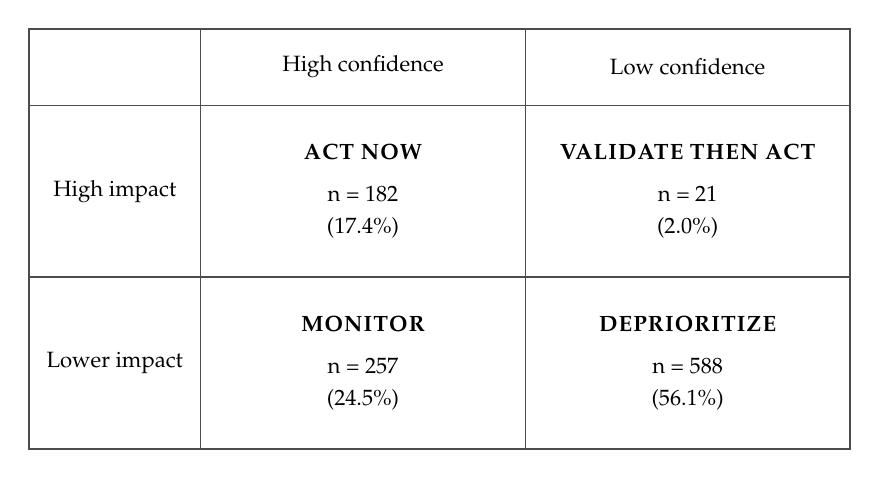
\begin{tikzpicture}

  % ---- sizing knobs ----
  \pgfmathsetlengthmacro{\AMcellw}{0.34*\linewidth}  % main cell width
  \pgfmathsetlengthmacro{\AMcellh}{0.18*\linewidth}  % main cell height
  \pgfmathsetlengthmacro{\AMhdrw}{0.18*\linewidth}   % left header column width
  \pgfmathsetlengthmacro{\AMhdrh}{0.08*\linewidth}   % top header row height

  % ---- derived geometry ----
  \pgfmathsetlengthmacro{\AMW}{\AMhdrw + 2*\AMcellw}
  \pgfmathsetlengthmacro{\AMH}{\AMhdrh + 2*\AMcellh}
  \pgfmathsetlengthmacro{\AMyMid}{\AMcellh}
  \pgfmathsetlengthmacro{\AMyTop}{2*\AMcellh}
  \pgfmathsetlengthmacro{\AMxLeft}{\AMhdrw}
  \pgfmathsetlengthmacro{\AMxMid}{\AMhdrw + \AMcellw}

  \definecolor{AMLine}{gray}{0.30}

  % ---- borders ----
  \draw[AMLine, line width=0.85pt] (0,0) rectangle (\AMW,\AMH);
  \draw[AMLine, line width=0.50pt] (\AMxLeft,0) -- (\AMxLeft,\AMH);
  \draw[AMLine, line width=0.50pt] (\AMxMid,0) -- (\AMxMid,\AMH);
  \draw[AMLine, line width=0.50pt] (0,\AMyMid) -- (\AMW,\AMyMid);
  \draw[AMLine, line width=0.50pt] (0,\AMyTop) -- (\AMW,\AMyTop);

  % ---- headers ----
  \node[align=center] at (\AMhdrw + 0.5*\AMcellw, \AMyTop + 0.5*\AMhdrh) {\footnotesize High confidence};
  \node[align=center] at (\AMhdrw + 1.5*\AMcellw, \AMyTop + 0.5*\AMhdrh) {\footnotesize Low confidence};

  \node[align=center] at (0.5*\AMhdrw, 1.5*\AMcellh) {\footnotesize High impact};
  \node[align=center] at (0.5*\AMhdrw, 0.5*\AMcellh) {\footnotesize Lower impact};

  % ---- cell text ----
  \tikzset{celltext/.style={align=center, inner sep=0pt}}

  % TOP-LEFT: ACT NOW
  \node[celltext] at (\AMhdrw + 0.5*\AMcellw, 1.5*\AMcellh) {%
    {\bfseries\footnotesize\scshape ACT NOW}\\[1.1mm]
    {\footnotesize n = 182}\\[-0.2mm]
    {\footnotesize (17.4\%)}%
  };

  % TOP-RIGHT: VALIDATE THEN ACT
  \node[celltext] at (\AMhdrw + 1.5*\AMcellw, 1.5*\AMcellh) {%
    {\bfseries\footnotesize\scshape VALIDATE THEN ACT}\\[1.1mm]
    {\footnotesize n = 21}\\[-0.2mm]
    {\footnotesize (2.0\%)}%
  };

  % BOTTOM-LEFT: MONITOR
  \node[celltext] at (\AMhdrw + 0.5*\AMcellw, 0.5*\AMcellh) {%
    {\bfseries\footnotesize\scshape MONITOR}\\[1.1mm]
    {\footnotesize n = 257}\\[-0.2mm]
    {\footnotesize (24.5\%)}%
  };

  % BOTTOM-RIGHT: DEPRIORITIZE
  \node[celltext] at (\AMhdrw + 1.5*\AMcellw, 0.5*\AMcellh) {%
    {\bfseries\footnotesize\scshape DEPRIORITIZE}\\[1.1mm]
    {\footnotesize n = 588}\\[-0.2mm]
    {\footnotesize (56.1\%)}%
  };

\end{tikzpicture}




  \captionsetup{justification=raggedright,singlelinecheck=false}
  \caption*{\footnotesize \textit{Note}. This matrix translates structural severity estimates into a decision-oriented triage for the locked graph using the disclosed, empirical, and augmented evidence views. Cells partition the cross-view high-impact candidate universe ($N=1{,}048$) by \textit{impact} (high vs. low) and \textit{evidence confidence} (high vs. low). Impact is based on the primary deny metric, $H1_{\log}$, which weights prime endpoints by log-obligations and measures the loss of semiconductor support under counterfactual removals. Evidence confidence reflects cross-view presence: low-confidence cases appear in only one view and are therefore more view-dependent. This matrix bins only impact and confidence. Semiconductor relevance is enforced downstream through the strict value-chain lens used to construct Table~\ref{tab:ch4_strict_top25}, while semantically uncertain candidates are tracked separately for validation in Appendix~\ref{app:c3_adjacent_uncertain_validation}.}
\end{figure}

Read Figure~\ref{fig:ch4_action_matrix} as a four-way triage for decision use. \textsc{Act now} denotes candidates that are high impact and high confidence. These are nodes whose removal yields a large deny severity and whose placement is supported by at least two evidence views, so the finding is not tied to a single visibility regime. \textsc{Validate then act} denotes candidates that are high impact but low confidence. These nodes appear severe in only one view, which often implies that their importance depends on view-specific routing that can change when additional evidence is admitted. For example, a firm may appear to control many semi$\rightarrow$prime routes in one view, but fall out of the high-impact set once shipping evidence or predicted links reveal alternative pathways. In these cases, the appropriate posture is to corroborate through targeted supplier discovery and adjudication before committing to mitigation. \textsc{Monitor} denotes candidates that are lower-impact but cross-view stable, making them persistent second-order leverage points worth tracking. \textsc{Deprioritize} denotes candidates that are both lower impact and view-dependent, where neither the estimated consequence nor the evidence warrants attention under a constrained decision budget. This matrix bins only impact and confidence. Semiconductor relevance is applied downstream, using the strict lens output to construct the chokepoint shortlist reported in Table~\ref{tab:ch4_strict_top25}.

% ---------- Table 4.2: Top-25 value-chain chokepoints ----------
\begin{table}[tbp]
  \centering
  \caption[\textit{Top-25 value-chain chokepoints}]{\textit{Top-25 value-chain chokepoints}}
  \label{tab:ch4_strict_top25}

  \footnotesize
  \setlength{\tabcolsep}{6pt}
  \renewcommand{\arraystretch}{1.04}

  % =======================
% Table 4.2 (tabular only, lean main-text)
% Strict observed Top-25 value-chain chokepoints
% =======================
\begin{tabularx}{\textwidth}{@{}c
  >{\hsize=1.0\hsize\raggedright\arraybackslash}X
  >{\hsize=1.0\hsize\raggedright\arraybackslash}X
  c
  S[table-format=1.4]@{}}
\toprule
Rank & Firm & Role & Corridor & {$H1_{\log}$} \\
\midrule
1  & TE Connectivity Plc & electronics interconnect & Near-prime & 0.0041 \\
2  & Comer Industries SpA & industrial components & Corridor & 0.0028 \\
3  & Aten International Co., Ltd. & electronics distribution & Corridor & 0.0026 \\
4  & Hurco Cos., Inc. & machine tools & Corridor & 0.0025 \\
5  & Hagener Feinstahl Bender & specialty metals & Corridor & 0.0024 \\
6  & George Risk Industries, Inc. & industrial controls & Corridor & 0.0023 \\
7  & Airgain, Inc. & RF components & Near-prime & 0.0021 \\
8  & Codan Ltd. & electronics systems & Corridor & 0.0021 \\
9  & D-Box Technologies, Inc. & electromechanical systems & Corridor & 0.0020 \\
10 & Velodyne Lidar, Inc. & sensing hardware & Near-prime & 0.0018 \\
11 & Aubert \& Duval SAS & specialty alloys & Corridor & 0.0017 \\
12 & Titomic Ltd. & advanced manufacturing & Corridor & 0.0016 \\
13 & Aspen Technology, Inc. & manufacturing software & Corridor & 0.0015 \\
14 & Arotech Corp. & defense electronics & Corridor & 0.0015 \\
15 & Quanta Computer, Inc. & EMS/ODM services & Corridor & 0.0014 \\
16 & Impinj, Inc. & semiconductor-enabled devices & Near-prime & 0.0014 \\
17 & Liebherr-International AG & industrial machinery & Corridor & 0.0013 \\
18 & ADTRAN Holdings, Inc. & communications hardware & Corridor & 0.0012 \\
19 & Metso Corp. & industrial equipment & Corridor & 0.0012 \\
20 & China International Marine & industrial manufacturing & Corridor & 0.0012 \\
21 & Vivotek Inc. & vision/security hardware & Corridor & 0.0012 \\
22 & D-Wave Quantum, Inc. & compute systems & Near-prime & 0.0012 \\
23 & Airbus SE & platform integrator & Corridor & 0.0011 \\
24 & Zhejiang Hailiang Co. Ltd. & primary metals & Corridor & 0.0011 \\
25 & Nordic Semiconductor ASA & fabless semiconductor & Near-prime & 0.0011 \\
\bottomrule
\end{tabularx}


  \captionsetup{justification=raggedright,singlelinecheck=false}
  \caption*{\footnotesize \textit{Note}. This table reports the 25 most structurally consequential nodes under the empirical view (including disclosed SCR ties and observed shipping) after applying the semiconductor value-chain strict relevance lens. Rows are ranked by $H1_{\log}$, the section's primary \textit{deny} severity metric. ``Corridor'' indicates nodes embedded in the empirically supported semi$\rightarrow$prime corridor. ``Near'' indicates nodes one step upstream of primes within that corridor definition. Role labels are interpretive and do not affect ranking.}
\end{table}

Table~\ref{tab:ch4_strict_top25} reports the semiconductor value-chain chokepoint shortlist sufficient for decision use. Figure~\ref{fig:ch4_action_matrix} is an impact and confidence triage over a cross-view high-impact universe, and it does not enforce semiconductor relevance. As a result, even candidates that fall in \textsc{Act now} can include firms that are structurally consequential but semantically adjacent to semiconductor continuity, such as generic enabling vendors that sit near primes. The strict relevance lens is therefore applied before promoting any firm as a semiconductor chokepoint. Table~\ref{tab:ch4_strict_top25} starts from the empirical-view single-node removal impacts, restricts the reporting universe to the strict value-chain stream produced by the codebook and corridor gate, and ranks rows by $H1_{\log}$, the log-obligation-weighted loss of semiconductor support to DoD Tier-1 prime endpoints under counterfactual single-node removal. The corridor label indicates whether a firm sits inside the empirically supported semi$\rightarrow$prime corridor and, when applicable, whether it is Near-prime or a corridor intermediary. Role labels summarize the mapped value-chain role and are interpretive. The confidence label in this table is specific to the strict Top-25 export. It is computed from cross-view presence within the strict Top-25 across disclosed, empirical, and augmented views and is reported as High, Medium, or Low. High-impact candidates that are structurally consequential but semantically uncertain are retained as a validation queue and documented separately in Appendix~\ref{app:c3_adjacent_uncertain_validation}.

To make the decision outputs concrete, the next step visualizes a representative local corridor neighborhood around a strict Top-25 chokepoint. It shows how single-node removal degrades prime-facing semiconductor support even when full disconnection is limited (Figure~\ref{fig:ch4_case_study_network_observed}).

Taken together, Figure~\ref{fig:ch4_action_matrix} and Table~\ref{tab:ch4_strict_top25} provide a conservative decision layer that keeps the estimand fixed while making uncertainty and semantics legible. The action matrix separates impact from stability, so high-impact, view-dependent cases are not mistaken for decision-ready chokepoints. The strict Top-25 table applies the semiconductor relevance lens to produce a semantically defensible shortlist for mitigation planning in the empirical baseline, while preserving a transparent record of excluded but consequential candidates in Appendix~\ref{app:c3_adjacent_uncertain_validation}. The next section grounds these decision outputs with an illustrative visualization and then documents robustness and interpretive limits.

%========================
% Section 4.7
%========================
\section{Robustness and Interpretive Limits}
\label{sec:ch4_robustness}

This section bounds how the decision outputs in \S\ref{sec:ch4_decision} should be interpreted under evidence uncertainty. The discussion first grounds the decision layer with an illustrative visualization that makes corridor degradation legible in the empirical view (Figure~\ref{fig:ch4_case_study_network_observed}), then summarizes the robustness and confidence diagnostics that support the uncertainty posture and states the key interpretive limits of the node-removal operator and the deny and delay metrics. The aim is to keep the results decision-useful without implying likelihood, intent, or item-level provenance.

Figure~\ref{fig:ch4_case_study_network_observed} provides a concrete view of what a high-impact chokepoint looks like inside the empirical dependency fabric. The focal node is selected from the strict empirical Top-25 list in Table~\ref{tab:ch4_strict_top25}, and a compact neighborhood is extracted using a deterministic corridor-based rule, so that the example is not hand-picked for effect. Panel~A shows the local subgraph under the empirical view before disruption. Panel~B shows the same node set under an identical layout after removing the focal node and its incident ties. The diagram is illustrative and local, not a rendering of the full Section~\ref{chap:network_analysis} network. Edges are shown without direction for readability.

% ---------- Figure 4.5: Illustrative local subgraph  ----------
\begin{figure}[tbp]
  \centering
  \caption[\textit{Illustrative local DoD-linked subgraph}]
  {\textit{Illustrative local DoD-linked subgraph}}
  \label{fig:ch4_case_study_network_observed}

  
\includegraphics[width=\linewidth]{report/figures/fig_4.5_case_study_network_observed.pdf}

  \captionsetup{justification=raggedright,singlelinecheck=false}
  \caption*{\footnotesize \textit{Note}. This figure visualizes the mechanism quantified in Figures~\ref{fig:ch4_robustness_empirical} and~\ref{fig:ch4_mechanism_decomposition} and summarized in Tables~\ref{tab:ch4_interdiction_performance_observed} and~\ref{tab:ch4_strict_top25}. The diagram is an illustrative local subgraph extracted from the empirical evidence view (disclosed SCR ties plus observed shipping), not the full Section~\ref{chap:network_analysis} network. Panel~A shows a compact DoD-linked neighborhood anchored on the DoD Tier-0 component \textit{Department of the Navy} and centered on the focal chokepoint \textit{TE Connectivity}; Panel~B shows the same node set under an identical layout after removing the focal node and its incident edges (the red $\times$ marks its former location). Edges represent supply-like dependency ties and are rendered without direction for readability; darker edges highlight the corridor paths used to define the local corridor neighborhood, while lighter edges provide surrounding context. The rendered subgraph contains 130 nodes and 449 edges, including 18 strict semiconductor nodes and 16 selected prime endpoints. In this local neighborhood, focal removal fully disconnects 0 selected primes but degrades 16 (orange outlines): each remains reachable but with fewer supporting semiconductor paths and/or longer remaining shortest paths. Accordingly, the figure is intended to illustrate how single-node disruption can generate widespread \textit{delay/fragility} effects even when complete denial is limited in a given neighborhood.}
\end{figure}

After focal removal, most selected prime endpoints in this neighborhood remain reachable from at least one strict semiconductor source, but many are degraded. The degradation takes two forms. First, fewer distinct semiconductor-to-prime support paths remain, reducing redundancy and increasing exposure to additional shocks. Second, the remaining routes are often longer or more circuitous, which is consistent with the section's delay and fragility interpretation even when complete disconnection is limited in a given neighborhood. This visualization clarifies what the action matrix and the Top-25 shortlist summarize at scale. High impact reflects measured consequence under node removal, and the mechanism often operates through corridor narrowing and route degradation rather than immediate cutoff alone.

\S\ref{sec:ch4_framework} defines the three evidence-conditioned views. Here they serve as a robustness frame. The empirical view is treated as the decision-grade baseline, with disclosed and augmented as uncertainty-conditioning comparisons. Appendix~\ref{app:c1_cross_view_stability} and Appendix~\ref{app:c2_stability_confidence_diagnostics} audit how evidence admission changes top-tail membership and ordering under the same estimand and node-removal operator. In the augmented view, predicted links function as visibility-expansion prompts for validation rather than confirmed dependencies.

Appendix~\ref{app:c1_cross_view_stability} shows that admitting shipping evidence refines but does not rewrite the highest-impact tail. In the top 25, the disclosed and empirical sets share 22 overlapping nodes, and their ordering is highly consistent across the common ranked set. In contrast, overlap involving the augmented view is low at small $N$ and ordered agreement is weaker. This pattern is expected when predicted links expand feasible routing, thereby changing which nodes appear most consequential at the very top. It does not imply that the augmented view is inherently more trustworthy than the empirical baseline. The augmented view is treated as a sensitivity regime that flags where additional supplier discovery could plausibly change prioritization. For the full overlap curves and rank stability summaries across increasing Top-$N$ thresholds, see Figure~\ref{fig:app_c1_cross_view_overlap} and Table~\ref{tab:app_c1_crossview_stability_summary}.

Confidence appears in three places in this section, and the labels refer to cross-view stability rather than probability. In Figure~\ref{fig:ch4_action_matrix}, confidence is a binary presence screen used for triage. A candidate is classified as high confidence if it appears in the cross-view Top-$N$ universe in at least two views. In Appendix~\ref{app:c2_stability_confidence_diagnostics}, a three-tier version of the same idea is reported for the high-impact set, based on presence in three views, two views, or one view. In Table~\ref{tab:ch4_strict_top25}, a High, Medium, Low label computed within the strict Top-25 shortlist after applying the relevance lens is reported. These schemes are related, but they are not numerically interchangeable because they are computed over different candidate universes and serve different reporting purposes. In all cases, confidence is a guide for decision posture. It is not a probability of disruption, and it is not proof of any single supplier relationship.

Semantic uncertainty is handled through a conservative reporting rule rather than by discarding inconvenient cases. The strict Top-25 shortlist in Table~\ref{tab:ch4_strict_top25} applies the semiconductor relevance lens before promoting any firm as a value-chain chokepoint. A concrete example from the empirical run is Microsoft Corp. In the adjacent/uncertain stream, Microsoft is structurally high-impact (rank 1 in that stream, with single-node deny impact $H1_{\log}=0.0093$) and sits inside the tier~2--3 corridor. It also passes the empirical two-sided corridor gate, meaning it lies on at least one empirical support route that connects a strict semiconductor source to a DoD Tier-1 prime. Passing this gate is necessary but not sufficient for strict value-chain promotion. The industry-code evidence must also map cleanly to a semiconductor value-chain role.

In this case, the relevance procedure records an uncertain classification under the codebook rules, so Microsoft is not promoted into the strict value-chain Top-25. This is not surprising for a large enterprise software and cloud services provider. Its industry codes primarily signal general IT and business enablement rather than a semiconductor value-chain role, so the observed corridor position could reflect prime operational dependence without being semiconductor-specific support. Instead, it is retained as a validation priority where the next step is to adjudicate whether the observed dependency reflects semiconductor-specific support or a general enterprise enablement relationship that is consequential for primes but not specific to semiconductor continuity. The specific industry-code triggers that produced the adjacent/uncertain classification are reported as ``Code basis'' in Appendix~\ref{app:c3_adjacent_uncertain_validation}. Appendix~\ref{app:c3_adjacent_uncertain_validation} documents these adjacent/uncertain high-impact cases and how they should be handled before they are treated as confirmed value-chain chokepoints.

Node removal and the section's severity metrics are intentionally conservative structural operators and have limits that matter for decision-making. Removing a firm represents generic unavailability and does not model inventories, substitution, rerouting through alternative suppliers, or recovery time. The deny metric, $H1_{\log}$, captures support loss under reachability and should be read as a consequence measure conditional on outage rather than a forecast of realized disruption. The delay metric, $H2$, captures structural path-length pressure among surviving semiconductor-to-prime routes rather than calendar delay. It can also exhibit a compositional effect because longer routes often disconnect first, thereby lowering the mean path length among the routes that remain, even as overall harm increases. $H2$ is therefore interpreted jointly with disconnect share and with the qualitative mechanism in Figure~\ref{fig:ch4_case_study_network_observed}. Together, these caveats support a disciplined reading of the decision layer. The action matrix provides an impact and stability triage. Table~\ref{tab:ch4_strict_top25} provides a relevance-constrained shortlist for mitigation planning. Appendix~\ref{app:c3_adjacent_uncertain_validation} provides the validation queue for semantically ambiguous but structurally consequential cases.

With these guardrails in place, the section's results remain decision-useful without overclaiming. Stable, high-impact findings in the empirical baseline support near-term action on continuity risk reduction and monitoring, while view-dependent high-impact cases motivate targeted supplier discovery and traceability work before action. The strict Top-25 shortlist should be understood as a conservative set of value-chain-plausible chokepoints conditional on disruption, not as a claim about the most likely targets or the only relevant dependencies. One additional robustness dimension is deferred: temporal stability, which would test whether rankings shift materially under alternative graph-snapshot dates. Because that analysis requires additional historical graph builds beyond the current frozen snapshot, it is reserved for future work. \S\ref{sec:ch4_synthesis} synthesizes these findings and translates them into the section's final decision takeaways.

%========================
% Section 4.8
%========================
\section{Synthesis and Decision Use}
\label{sec:ch4_synthesis}

This section closes the analysis by making the results legible and actionable without requiring network-science fluency. It is intentionally not a recap of \S\ref{sec:ch4_severity}--\S\ref{sec:ch4_robustness}. Instead, the analysis is translated into a simple workflow that explains what the outputs mean in real operational terms. Figure~\ref{fig:ch4_action_matrix} presents the first filter, separating high-consequence findings that are stable across evidence views from those that are view-dependent and therefore require validation. Table~\ref{tab:ch4_strict_top25} then supplies the conservative starting shortlist of value-chain-plausible chokepoints in the empirical baseline for mitigation planning and monitoring. Appendix~\ref{app:c3_adjacent_uncertain_validation} records the cases that are structurally consequential but semantically uncertain and converts them into a disciplined validation queue rather than treating them as headline chokepoints.

The central question is how much semiconductor-relevant support DoD Tier-1 primes would lose or degrade, purely because of network structure, if any single firm in the DoD-linked dependency network were unavailable. The answer comes from a disciplined set of ``what if this firm goes offline'' stress tests on a locked dependency map. Holding the Section~\ref{chap:dod-supply-chain} object fixed, one firm at a time is removed, and how semiconductor support can still reach prime endpoints through the remaining network is recomputed. In real terms, the question is whether an outage collapses many routes at once, forces support onto fewer and more fragile detours, or eliminates all viable routes into a prime. Figure~\ref{fig:ch4_case_study_network_observed} provides a concrete illustration. Removing a single corridor node can degrade many endpoints at once, even when no endpoint is cleanly disconnected in that local view. The decision layer in Figure~\ref{fig:ch4_action_matrix} then translates these consequences into a posture for action versus validation under evidence uncertainty. Throughout, the posture is conditional. The analysis assesses the consequences if a disruption occurs, not who will be disrupted, when it will occur, or how likely any hazard is to materialize.

This decision translation carries through two failure modes that matter in practice: denial and delay. Denial is the hard case. A prime effectively loses semiconductor support because no viable support route remains from the strict semiconductor source set into that endpoint. Concretely, this appears to be a forced stop, an immediate scramble for substitutes, or a rapid drawdown of inventories while the program searches for an alternative qualified source. Delay is the softer but often more operationally plausible case. A prime is not fully cut off, but the remaining support routes become fewer, thinner, and more circuitous. In real terms, that means longer lead times, more handoffs across intermediate firms, less slack to absorb routine hiccups, and a higher chance that a follow-on disruption tips a merely degraded situation into outright denial. Figure~\ref{fig:ch4_case_study_network_observed} is the intuition anchor for this distinction. A single removal can leave endpoints nominally connected while degrading many of them at once by collapsing redundant routes and forcing the remaining routes onto longer or more brittle paths. That is also why delay severity is interpreted jointly with disconnect share in Table~\ref{tab:ch4_interdiction_performance_observed} rather than treating any one metric as a standalone statement about calendar time.

Figure~\ref{fig:ch4_action_matrix} is the first decision filter because it tests whether a high-consequence finding persists when the evidence admitted into the same locked network is varied. Read the matrix as triage under uncertainty. In the \textsc{Act now} cell, the result is both consequential and stable across evidence views, so it is less likely to be an artifact of missing visibility and more suitable to treat as a planning assumption. In the \textsc{Validate then act} cell, the result is consequential but view-dependent, which means it can be driven by a particular routing picture that changes once additional relationship evidence is admitted. Put differently, these are the cases in which the next step is not an immediate mitigation investment. The next step is to verify the actual dependency through supplier discovery and adjudication. Appendix~\ref{app:c1_cross_view_stability} and Appendix~\ref{app:c2_stability_confidence_diagnostics} provide the audit trail for this posture by showing how top-tail membership and ordering move across the disclosed, empirical, and augmented views.

Table~\ref{tab:ch4_strict_top25} is the conservative ``start here'' output for decision use. It is conservative in two ways. First, it is anchored on the empirical evidence view, which pairs disclosed relationships with observed shipping and serves as the section's decision-grade baseline. Second, it applies the strict semiconductor relevance lens before promoting any firm as a value-chain chokepoint. For a planner, this list is meant to support concrete continuity work. It identifies a small set of named firms for which an outage would impose disproportionate downstream consequences in this DoD-linked dependency environment, conditional on disruption. It is not a forecast of likely targets. It is not a complete inventory of all dependencies that matter to DoD mission performance. It is not item-level provenance tracing into specific platforms. The decision value is prioritization under constraint. If a planner can only monitor, engage, or harden a limited number of positions, Table~\ref{tab:ch4_strict_top25} provides the section's most defensible shortlist for the empirical baseline. At the same time, Figure~\ref{fig:ch4_action_matrix} preserves the broader triage context in which that shortlist sits.

Appendix~\ref{app:c3_adjacent_uncertain_validation} contains the cases that are structurally consequential in the dependency fabric but not yet defensible to label as semiconductor value-chain chokepoints. This queue prevents two common decision errors. The first is silently discarding high-impact findings because their industry codes look generic. The second is promoting them as ``semiconductor chokepoints'' when the evidence supports consequence but not value-chain role. A concrete example is the kind of enterprise software or cloud services provider that can sit close to primes and appear on important support routes. That position can be consequential for prime operations while remaining ambiguous as semiconductor-specific support. In the workflow implied by Figure~\ref{fig:ch4_action_matrix}, these cases belong in \textsc{Validate then act}. The immediate task is adjudication, not mitigation. Operationally, this means targeted supplier discovery, contract and dependency clarification, and traceability-oriented verification to determine whether the observed relationship reflects semiconductor-relevant enabling capacity or general enterprise enablement that should be handled through a different continuity lens.

The second attack surface in \S\ref{sec:ch4_upstream} changes how continuity planning should be conceived because it shows how harm can accumulate without a clean cutoff. Even when primes remain nominally supported, disruption can make the semiconductor production and replenishment base brittle by shrinking the upstream support ecosystem on which semiconductor firms rely, leaving fewer redundant routes. In real terms, this is the scenario where the system ``still works,'' but it works on fewer options, with less slack, and with more single points of failure outside the immediate prime-facing view. Lead times stretch, substitutions become harder to execute quickly, and routine perturbations that would normally be absorbed start to cascade as fewer redundant routes remain to carry the load. This does not overturn the corridor story. In this DoD-anchored object, semiconductor-side leverage largely maps back onto near-prime and corridor-adjacent positions rather than implying that distance-to-prime tiers dominate. The decision implication is therefore additive. Corridor chokepoints anchor efforts to prevent outright denial. At the same time, semiconductor-side brittleness poses a parallel planning problem, motivating validation and resilience efforts to reduce degradation and compounding-shock risk.

Taken together, the section's outputs support a simple decision workflow under constrained attention and imperfect visibility. The workflow starts with posture. The action matrix separates findings that are both consequential and stable from findings that are consequential but sensitive to what evidence is visible. Relevance discipline is then applied, so the result is not just a list of structurally important firms, but a defensible set of semiconductor value-chain chokepoints for reporting and mitigation planning. Finally, the remaining high-impact yet ambiguous cases are treated as a structured work plan for supplier discovery and adjudication rather than as noise. This workflow tells a decision-maker what to harden and monitor first, what to verify before committing resources, and what to treat as second-order but persistent leverage points. That translation from raw rankings to an ``act, validate, monitor'' posture is the primary decision output of this section.

Two extensions are reserved for the integrative discussion in Section~\ref{chap:from_illumination_to_assurance}. First, the corridor chokepoints identified here for continuity risk also represent high-leverage positions for integrity attacks---counterfeits, hardware Trojans, and toolchain tampering concentrate at the same structural bottlenecks---and the policy implications of that overlap are developed there. Second, the severity scores reported here measure structural consequence $S(n)$ only. Illustrative probability scenarios---for example, how the action-matrix priorities would shift if nodes in geopolitically exposed regions carry elevated disruption likelihood $P(n)$---require assumptions beyond the structural analysis and are explored in Section~\ref{chap:from_illumination_to_assurance} as part of the policy discussion.

Section~\ref{chap:from_illumination_to_assurance} shifts from measurement to policy design. Building on the decision workflow from Section~\ref{chap:network_analysis}, the identified high-consequence positions and the structured validation agenda are translated into a set of actionable policy and regulatory recommendations for the Department of Defense. The focus is on how DoD can reduce supply-chain opacity in ways that are realistic for acquisition and oversight, including traceability and provenance practices that make critical dependencies auditable across tiers and over time. The goal is not perfect transparency. It is decision-grade visibility that enables the DoD to verify the dependencies that matter, detect emerging chokepoints early, and make the semiconductor supply chain more defensible against denial and delay in a crisis.
% chktex-file 8   en-dash compounds are correct academic usage
% chktex-file 24  \label on own line is standard practice
% chktex-file 36  acronym parentheses (OUSD(A&S)) need no leading space
% chktex-file 38  American-style punctuation inside closing quotes is correct
\chapter{From Illumination to Assurance}
\label{chap:from_illumination_to_assurance}

This section translates the report's empirical findings into a policy agenda for reducing opacity in the Department of Defense semiconductor supply chain. Sections~\ref{chap:intro} through~\ref{chap:network_analysis} established the strategic stakes of semiconductor dependence, constructed a DoD-anchored multi-tier network from disclosed, predicted, and observed evidence, and identified high-consequence positions within that network using structural analysis and disruption testing. The task of Section~\ref{chap:from_illumination_to_assurance} is different. Rather than asking what the network looks like or which nodes matter most, this section asks what the Department of Defense and Congress should do with those findings.

The earlier sections show that it is possible to generate a decision-grade map of DoD-relevant semiconductor dependencies from unclassified and commercially available data. That map is auditable, reproducible, and useful for prioritization. It reveals hidden tiers, identifies chokepoints, and supports a structured workflow for deciding what to act on, what to validate, and what to monitor. At the same time, this report also demonstrates the limits of that achievement. The resulting network is not a complete census of the defense semiconductor supply chain. It is a defensible snapshot built from evidence streams that are themselves partial, uneven, and differently constrained. Residual opacity is not simply a flaw in the data. It is one of this report's core findings.

The policy problem that follows from this finding is clear. The Department of Defense cannot rely indefinitely on reverse-engineering its supply chain after the fact, whether through commercial illumination tools, episodic surveys, or one-off analytic efforts. Those approaches can improve visibility, but they do not alter the institutional conditions that generate opacity in the first place. Critical dependencies remain hidden because they are not systematically captured when suppliers are brought into a program, and they are not consistently updated as designs change, parts are substituted, ownership shifts, or production arrangements move across firms and borders. The issue, therefore, is not only how to see more. It is how to make the dependencies that matter more auditable across tiers and over time.

This section does not argue that the Department lacks regulations, priorities, or pilot authorities touching supplier assurance, program protection, lifecycle sustainment, counterfeit avoidance, or supply-chain monitoring. Existing policy already addresses mission-critical functions and trusted systems, lifecycle acquisition risk, diminishing manufacturing sources and material shortages (DMSMS), counterfeit electronic parts, and pilot supply-chain mapping efforts \parencite{ch5_dodi520044,ch5_dodi500085,ch5_tpp_guidebook_2022,ch5_dodi424515,ch5_dmsms_contract_language_guidebook,ch5_dfars2522467007,ch5_dfars2522467008,ch5_dfars2522047020,ch5_ndaa2024_sec856}. The argument is narrower and more consequential. The Department still lacks a coherent targeting and operating model for using those authorities to create decision-grade visibility for high-consequence semiconductor dependencies. The binding constraint is not whether the Department cares about supply chains. It is whether the Department can require the right evidence, from the right actors, at the right points in the lifecycle, and with the right validation priority \parencite{ch5_dod2022_supplychains,U.S.GovernmentAccountabilityOffice2025}.

The objective of this section is not perfect transparency. It is decision-grade visibility: a level of visibility sufficient to identify high-consequence dependencies, verify them when necessary, monitor meaningful change, and support timely intervention in the face of continuity and integrity risk. That standard is narrower than full supply-chain transparency but more demanding than retrospective illumination. It requires the Department to know enough, with sufficient confidence, to distinguish between what must be hardened immediately, what must be validated before action, and what can be monitored over time. The policy goal of this section is therefore fully continuous with the empirical goal of Section~\ref{chap:network_analysis}.

The core claim that follows from Sections~1--4 is therefore not that the Department needs another generic reporting rule. It is that the binding constraint is institutional evidence production. Illumination can prioritize where the Department should look, but assurance requires auditable objects: standardized, minimally disclosed evidence that can be required at specific acquisition touchpoints, refreshed when dependencies are rewired, and protected through controlled access. The recommendations in this section are therefore framed in terms of deliverables, triggers, responsibilities, and verification pathways rather than a mandated vendor or a single technical stack \parencite{ch5_nist800161r1upd1,ch5_dodi520044}.

To keep the recommendations realistic and coherent with the evidence presented thus far, this section focuses on acquisition, oversight, and traceability levers rather than prescribing a single technical architecture or arguing for universal disclosure of all supplier relationships. The emphasis is on policy requirements, governance principles, and institutional mechanisms that could reduce opacity while preserving legitimate protections for proprietary information and trade secrets. The focus remains defense-relevant semiconductor dependencies rather than the entire defense industrial base. The broader conclusion, including the project's overall limitations and future work, is reserved for Section~\ref{chap:conclusion}.

The remainder of Section~\ref{chap:from_illumination_to_assurance} proceeds in stages. Section~\ref{sec:ch5_decision_grade_illumination_limits} explains what Sections~1 through~4 accomplish and why a residual visibility ceiling remains. Section~\ref{sec:ch5_policy_objectives_design_principles} then formalizes the policy objective and design principles that should govern any credible effort to reduce supply-chain opacity under partial observability. Section~\ref{sec:ch5_layered_assurance_framework} translates those principles into a layered assurance framework that distinguishes traceability, provenance, resilience, and decision integration. The sections that follow operationalize this framework through acquisition and regulatory levers, data-governance choices, incentive and enforcement mechanisms, an implementation roadmap, and a set of specific recommendations for the Department of Defense and Congress. Throughout, this section uses the Section~\ref{chap:network_analysis} act-now, validate-then-act, and monitor workflow as the bridge between structural analysis and policy design.

%========================
% Section 5.1
%========================
\section{Decision-Grade Illumination and Its Limits}
\label{sec:ch5_decision_grade_illumination_limits}

This section is diagnostic. It summarizes what Sections~1--4 deliver for decision use and explains why a residual visibility ceiling remains even under a provenance-aware, decision-grade build. The section begins by identifying two core outputs that carry forward into policy design. The first is an auditable dependency map of DoD-relevant semiconductor relationships that records whether each tie is disclosed, predicted, or supported by observed shipping evidence. The second is a constrained decision workflow that translates structural rankings into an ``act now,'' ``validate then act,'' ``monitor,'' and ``deprioritize'' posture. This section also states what these outputs do not claim to provide. They are not a full census of the multi-tier supply chain; they do not trace specific components to specific defense platforms; and they do not directly test for integrity compromise. The visibility ceiling is then defined as the operational boundary produced by partial observability beyond Tier~1 and by limits in identity linkage at the demand anchor. The goal is to make the starting conditions for policy design explicit before Section~\ref{sec:ch5_policy_objectives_design_principles} formalizes the objectives and design principles that will govern credible recommendations. It also clarifies that the ceiling is not only a property of incomplete data. It is reinforced by a policy environment in which supplier visibility still sits across separate acquisition, sustainment, counterfeit, and program protection channels rather than a unified operating model \parencite{ch5_dod2022_supplychains,U.S.GovernmentAccountabilityOffice2025}.

Sections~\ref{chap:dod-supply-chain} and~\ref{chap:network_analysis} produce the main empirical output that this section builds on: a DoD-anchored map of who depends on whom in the semiconductor supply chain. The analysis starts from the firms the Department pays directly through prime contracts, then links those firms into the commercial identifier space to follow their upstream supplier relationships. The map is expanded using three kinds of evidence. Some links are disclosed in FactSet's Supply Chain Relationships data \parencite{factset_supply_2024}. Some links are added as high-confidence predictions from the Section~\ref{chap:link-prediction} models and are treated as hypotheses to be checked rather than facts. Some links are supported by observed shipping records, which provide transaction-style evidence that two firms exchanged goods at a point in time \parencite{factset_factset_2025}. For every link, the analysis retains a provenance tag that records which evidence stream supports it, so later analysis can distinguish what is directly evidenced from what is inferred. The result is auditable and reproducible, but it is still a defensible snapshot of DoD-relevant semiconductor dependencies rather than a complete census.

Section~\ref{chap:network_analysis} then uses this locked map to identify where continuity risk concentrates and what kinds of disruptions would matter most if they occurred. The analysis treats risk as a consequence problem rather than a forecasting problem. The analysis asks what happens to DoD-linked continuity when certain firms become unavailable or when paths through the network degrade, and compares targeted disruptions to a random-outage baseline. This stress-testing approach surfaces high-leverage positions such as chokepoints, bridges, and corridor intermediaries that sit on many dependency pathways. It also shows that some findings are robust across evidence views, while others shift when additional evidence layers are admitted. That stability check is part of what makes the output actionable because it separates results that can support immediate action from results that require follow-on validation work.

A ranking by itself is not yet a decision, so Section~\ref{chap:network_analysis} translates the stress-test results into a constrained workflow that matches how the Department actually operates. The workflow combines two pieces of information. One is impact, meaning how damaging disruption would be if a firm or pathway failed. The other is evidence stability, meaning whether a high-impact finding holds across alternative evidence-conditioned views of the same locked network. ``Act now'' covers findings that are high-impact and stable, so they justify immediate attention even under partial observability. ``Validate then act'' covers findings that appear high-impact but shift across views, so they warrant targeted supplier discovery and adjudication before committing resources. ``Monitor'' captures positions that are not immediate priorities but remain structurally consequential enough to watch for movement as the network changes. ``Deprioritize'' is an explicit constraint choice that prevents scarce analytic and engagement capacity from being spread too thin. This workflow is the section's bridge from structure to governance because it makes uncertainty operational, and it specifies what kind of follow-on work is required when visibility is incomplete.

This report's outputs are decision-useful in part because they draw hard boundaries around what the evidence can support. The map is not a complete census of the defense semiconductor supply chain, and some portions of the demand surface fall outside the mapped universe when prime recipients cannot be reconciled into commercial identifier space. Predicted links are not treated as ground truth, even when they are high-confidence, because their role is to focus validation effort rather than to certify dependency. The observed shipping layer strengthens confidence that two firms exchanged goods at a point in time, but it is still event-level evidence, and it does not trace specific components into specific defense platforms. For the same reason, Section~\ref{chap:network_analysis} is principally a continuity and structural severity section. It does not directly test tampering or compromise, and integrity enters here only as an implication of the continuity--integrity framework introduced in Section~\ref{chap:intro}. These boundaries prevent a category error in which illumination is mistaken for assurance.

The term ``visibility ceiling'' describes the operational boundary beyond which dependency evidence is not reliably produced, reconciled, and refreshed in a form that supports audit and decision use. One part of the ceiling is relational. Many upstream ties are never disclosed, are disclosed unevenly, or are disclosed without the standardization needed to integrate them cleanly across tiers. Another part of the ceiling concerns identity linkage. Even when a firm is known to DoD through contracting, it may not be linkable to the commercial identifier space that enables upstream mapping, creating structural blind spots at the demand anchor. The observed shipping layer helps by adding event evidence that two firms exchanged goods, but it does not cover the full universe of exchanges, and it is not designed to certify platform-specific provenance. These constraints are consistent with an institutional reality in which visibility is strongest near Tier~1 and degrades beyond it, and in which change over time can rewire dependencies faster than evidence is captured. Those institutional mechanisms are treated as explanations for why even a careful snapshot remains incomplete, not as outcomes directly measured in the data. That institutional reading is consistent with current assessments that DoD visibility efforts remain limited below the top tiers, unevenly coordinated, and not yet backed by a coherent set of tested reporting requirements across the enterprise \parencite{U.S.GovernmentAccountabilityOffice2025}.

The ceiling is most visible in practice through the structure of the Section~\ref{chap:network_analysis} triage outputs, especially the size and character of the ``validate then act'' queue. When a high-impact finding is stable across evidence views, the ceiling binds less, and the workflow can justify immediate action. When a high-impact finding shifts across views, the ceiling binds more and the correct response is targeted adjudication, not increased confidence. The validation queue is not a defect in the analysis. It is a diagnostic artifact of partial observability that identifies where the Department needs additional supplier discovery, documentation, or verification to move from plausible leverage to defensible action. The ``monitor'' category reflects the temporal side of the ceiling. Even when current impact is modest, limited change detection means the Department must watch for meaningful rewiring that can elevate risk. ``Deprioritize'' serves the same diagnostic purpose by making constraint explicit and by preventing scarce capacity from being consumed by low-yield leads.

Under the continuity lens introduced in Section~\ref{chap:intro} and operationalized through the disruption tests in Section~\ref{chap:network_analysis}, the policy relevance of the visibility ceiling is that it increases the probability of surprise propagation. When high-leverage dependencies sit beyond what can be evidenced, the Department is more likely to encounter deny and delay cascades only after they begin to disrupt schedules and readiness. This report shows that structural severity is concentrated and that conservative evidence conditioning can separate stable priorities from sensitive ones, but it also shows that uncertainty does not disappear. Existing policy already recognizes adjacent versions of this problem through program protection, counterfeit avoidance, DMSMS management, and pilot supply-chain mapping, but those authorities do not yet operate as a unified targeting model for semiconductor dependencies \parencite{ch5_dodi520044,ch5_dodi424515,ch5_dfars2522467007,ch5_dfars2522467008,ch5_ndaa2024_sec856}. The highest-value policy problem is therefore not how to produce a perfect map, but how to lower the ceiling where it matters most by making verification faster, cheaper, and more routine for high-consequence dependencies within an existing but still fragmented policy environment \parencite{ch5_dod2022_supplychains,U.S.GovernmentAccountabilityOffice2025}. The continuity--integrity framework from Section~\ref{chap:intro} implies a parallel constraint for integrity assurance. Event-level evidence and inferred links can accelerate who to investigate first, but they cannot certify item history, substitution accountability, or chain-of-custody into specific platforms. This diagnostic conclusion sets up Section~\ref{sec:ch5_policy_objectives_design_principles}, which formalizes objectives and design principles for credible interventions under partial observability.

%========================
% Section 5.2
%========================
\section{Policy Objectives and Design Principles}
\label{sec:ch5_policy_objectives_design_principles}

Section~\ref{sec:ch5_decision_grade_illumination_limits} makes the starting conditions for policy design explicit. This report produces an auditable, provenance-aware map and a constrained act now, validate then act, monitor, and deprioritize workflow, but it also shows that a residual visibility ceiling remains because upstream dependencies are only partially disclosed, only partially linkable, and only partially observable through event-level evidence. The policy task that follows is therefore not to promise perfect transparency or universal disclosure. It is to specify what kind of visibility is necessary for defensible action when continuity and integrity consequences are highest. This section formalizes that objective and then states the design principles that should govern any credible effort to reduce opacity in the DoD semiconductor supply chain under partial observability. The principles that follow do not ask the Department to care about an entirely new class of problem. They specify how existing authorities and existing priorities can be used in a more targeted, auditable, and lifecycle-persistent way for semiconductor-relevant dependencies \parencite{ch5_dodi520044,ch5_nist800161r1upd1,ch5_dod2022_supplychains}.

The objective is decision-grade visibility: enough timely, verifiable information about high-consequence dependencies to support defensible action without requiring a complete census of every firm, tier, and transaction. This standard is narrower than full transparency, but more demanding than retrospective illumination after disruption costs have already materialized \parencite{ch5_nist800161r1upd1}. In practice, it must enable the Department to identify which dependencies matter most, verify relationships when the evidence is thin or contested, detect meaningful change as designs and suppliers shift, and trace back quickly when disruptions, anomalies, or suspected compromise emerge. This objective is operationally defined by the workflow in Section~\ref{chap:network_analysis} because the purpose of visibility is not knowledge for its own sake, but the ability to act now when impact and confidence justify it, validate then act when leverage is plausible but stability is weak, monitor when positions are consequential but not urgent, and deprioritize when additional inquiry is unlikely to change a decision. To make this objective actionable, the policy response is organized around six design principles.

This visibility standard is also not a single requirement because the Department's exposure is not a single risk. As Section~\ref{chap:intro} argued, continuity risk concerns deny and delay: disruptions, bottlenecks, and outages that propagate into schedule failure, readiness degradation, or production shortfalls. Integrity risk concerns compromise: tampering, substitution, counterfeit insertion, or other forms of degradation that undermine trusted performance. These two risk modes create different evidence needs. Continuity decisions are often driven by dependency structure, substitutability, and change detection, while integrity decisions require auditable history, provenance, and substitution accountability. The design principles below are therefore intended to support both lenses, and Section~\ref{sec:ch5_layered_assurance_framework} makes the mapping explicit by distinguishing traceability, provenance, resilience, and decision integration as separate assurance functions \parencite{ch5_dodi520044,ch5_dod2022_supplychains}.

Principle~1 is risk-tiered scoping. Policy should require the deepest visibility and the strongest verification where continuity and integrity consequences are highest, and it should relax those demands as consequence falls. The visibility ceiling documented in Section~\ref{sec:ch5_decision_grade_illumination_limits} makes blanket disclosure and documentation requirements self-defeating because they either fail outright or generate uneven reporting that cannot support decision use. Operationally useful visibility therefore depends on selective depth that aligns evidentiary demands to the act now, validate then act, monitor, and deprioritize posture. It concentrates scarce analytic capacity, supplier engagement, and verification effort on the dependencies that plausibly drive disruption cascades. Risk-tiered scoping is therefore not a concession to opacity. It is a disciplined allocation of assurance effort \parencite{ch5_nist800161r1upd1}. It is a governance requirement for moving from one-off illumination toward durable assurance.

Principle~2 is verifiability over self-attestation. Section~\ref{sec:ch5_decision_grade_illumination_limits} showed that this report's map gains decision value by distinguishing among evidence types rather than treating all reported relationships as equivalent. Disclosed relationships are useful and often highly informative, especially for illumination, prioritization, and initial triage. But when a dependency carries serious continuity or integrity consequences, disclosure alone may not be enough to justify intervention, resolve ambiguity, or adjudicate meaningful change over time. That posture is consistent with Section~\ref{chap:link-prediction}, which treats predicted links as hypotheses to be checked rather than as facts to be assumed. The policy lesson is therefore not that reported relationships are untrustworthy per se. It is that high-consequence action should rest, wherever possible, on evidence that can be corroborated, reconciled, and audited when the stakes are highest \parencite{ch5_nist800161r1upd1,ch5_dodi520044}.

Principle~3 is minimum necessary disclosure. A credible visibility regime should require access to the information needed for decision use, but no more than that. The problem is not simply that too little information is publicly available. It is that the information required for continuity and integrity decisions is not reliably available to the right actors in a usable form. That does not require unrestricted transparency across the full multi-tier supply chain. Prime contractors may need visibility sufficient to manage and validate the dependencies that affect their own delivery obligations, while the Department may need a broader oversight view into high-consequence dependencies that cut across firms, programs, and tiers. Other commercial details may remain protected when they are not necessary for governance, verification, or intervention. Preserving trade secrets and legitimate proprietary interests is not in tension with this visibility objective \parencite{ch5_nist800161r1upd1,ch5_dodi520044}. It is part of the design condition for any regime that firms can participate in without treating disclosure itself as a source of strategic loss.

Principle~4 is interoperability and machine-readable standardization. Auditable supply-chain visibility cannot scale if each program, prime, or office records dependencies in its own format, with its own identifiers, and on its own update cycle. As Section~\ref{sec:ch5_decision_grade_illumination_limits} makes clear, visibility breaks down when dependency evidence cannot be reliably produced, reconciled, and refreshed for decision use, and Section~\ref{chap:dod-supply-chain} shows how much work is required even in a research setting to align disclosed, predicted, and observed evidence into a common provenance-aware snapshot. A policy regime that reproduces fragmentation at the point of reporting would simply recreate that same integration problem inside government. The design requirement is therefore not a single centralized database or a monolithic platform. It is a common, machine-readable structure for recording, exchanging, and refreshing dependency evidence so it can be reconciled across firms, programs, and tiers. At minimum, that requires a consistent identifier strategy, a small standardized set of fields sufficient for decision use, and a shared method for recording consequential change over time. Without that minimum standardization, the Department simply recreates inside government the same integration burden documented in Sections~\ref{chap:link-prediction} through~\ref{chap:network_analysis} \parencite{ch5_nist800161r1upd1}.

Principle~5 is lifecycle persistence and meaningful change detection. Supply-chain visibility cannot be treated as a one-time reporting exercise because redesign, obsolescence responses, supplier substitutions, ownership changes, geographic relocations, and ordinary supplier churn repeatedly rewire semiconductor supply chains. This point follows directly from the diagnostic conclusion of Section~\ref{sec:ch5_decision_grade_illumination_limits}, which shows that even a careful build remains a provenance-aware snapshot rather than a complete census, and from Section~\ref{chap:dod-supply-chain}, which treats the network as a locked snapshot so that Section~\ref{chap:network_analysis} can distinguish structural findings from ongoing change. A credible policy response must therefore ensure that visibility persists after initial disclosure and captures changes that materially alter continuity or integrity exposure \parencite{ch5_dod2022_supplychains,ch5_dodi424515}. The requirement is not constant surveillance of every transaction. It is a regime with update logic that makes consequential rewiring visible soon enough to support reclassification, revalidation, and intervention when the risk posture changes.

Principle~6 is burden-aware implementation under conditions of indirect reach. Visibility is strongest near Tier~1 and degrades beyond it, meaning the Department usually encounters sub-tier dependencies through prime contractors rather than direct contractual control. Any credible regime must therefore be designed for the structure through which information actually moves, not for an idealized system in which the government can interrogate every firm on demand. That constraint is especially important for smaller suppliers, which may face disproportionate reporting and verification burdens even when they occupy consequential positions in the network. A defensible visibility regime will not be durable if it depends on uniform demands that overwhelm supplier capacity or encourage defensive, low-quality reporting. A feasible regime must instead be phased, selective, and proportionate so participation remains administratively manageable, and the resulting information is more likely to be accurate, timely, and decision-useful \parencite{ch5_dod2022_supplychains,ch5_usc2223}.

Taken together, these principles define what a credible response to the visibility ceiling should seek to achieve and what constraints it must respect. The objective is decision-grade visibility, meaning enough timely and verifiable information about high-consequence dependencies to support defensible action under partial observability. The six principles specify how that objective should be pursued. Visibility should be risk-tiered, evidence should be verifiable, disclosure should be limited to what decision use requires, information should be structured for interoperability, visibility should persist through meaningful change, and implementation should remain feasible under conditions of indirect reach. These are not recommendations in themselves. They are design constraints for using existing authorities in a more coherent and targeted way across the rest of Section~\ref{chap:from_illumination_to_assurance}. The next section translates them into a layered assurance framework that distinguishes traceability, provenance, resilience, and decision integration so the Department can connect visibility requirements to practical governance choices without demanding perfect transparency.

%========================
% Section 5.3
%========================
\section{A Layered Assurance Framework}
\label{sec:ch5_layered_assurance_framework}

Section~\ref{sec:ch5_policy_objectives_design_principles} defined the objective of decision-grade visibility and set out the principles that should govern any credible effort to reduce opacity in the DoD semiconductor supply chain. Those principles establish what a workable policy response must achieve, but they do not yet specify how visibility should be organized in practice once the Department moves from diagnosis to institutional design. The next step is therefore to distinguish the different functions that an assurance regime must perform under partial observability. Some are about following dependencies and movements, some are about establishing evidentiary history, some are about understanding whether critical dependencies can withstand disruption, and some are about translating that information into defensible action. Those functions are organized as a layered assurance framework built around traceability, provenance, resilience, and decision integration. That distinction matters because current DoD practice already touches these evidentiary functions, but often through separate channels such as program protection, counterfeit avoidance, sustainment management, and emerging supply-chain mapping \parencite{ch5_dodi520044,ch5_dfars2522467007,ch5_dfars2522467008,ch5_dfars2522047020,ch5_dodi424515,ch5_ndaa2024_sec856}.

A layered framework is necessary because the visibility ceiling described in Section~\ref{sec:ch5_decision_grade_illumination_limits} is not a single informational deficit. The Department must be able to determine that a dependency exists, reconstruct where it originated and how it changed, assess whether disruption can be absorbed or recovered from, and decide what kind of intervention the evidence justifies. Those are related tasks, but they are not identical, and they do not require the same kind or degree of proof. A generic call for greater transparency therefore obscures the central policy problem: matching different decision questions to the forms of visibility and verification they actually require. The value of a layered framework is that it separates those functions without severing their connection, so the Department can ask not only how much it sees but also what kind of evidence it has and what that evidence is sufficient to support.

The framework is organized around four distinct but connected layers. Traceability concerns the structured visibility of dependencies, movements, custody changes, and other relevant supply-chain events across firms, tiers, and time. Provenance concerns the evidentiary history attached to those relationships and movements, including questions of origin, transformation, substitution, and documentation. Resilience concerns the evidence needed to judge whether a dependency can absorb disruption, adapt under stress, or recover after failure. Decision integration concerns how those three layers are translated into the Section~\ref{chap:network_analysis} act now, validate then act, monitor, and deprioritize workflow. The layers are therefore complementary rather than interchangeable, because each answers a different policy question and supports a different part of the Department's assurance problem.

Layer~1 is traceability. Traceability is the structured ability to follow relevant dependencies, movements, custody changes, substitutions, and other consequential supply chain events across firms, tiers, and time \parencite{ch5_dod2022_supplychains,ch5_nist800161r1upd1}. Sections~\ref{chap:dod-supply-chain} and~\ref{chap:network_analysis} show why this layer is foundational. Even under partial observability, the ability to locate where dependencies sit, how they connect, and how they may be rewired is what makes chokepoints, corridor intermediaries, and concentrated exposures visible for continuity analysis. In policy terms, traceability answers the first-order questions of who depends on whom, where a relevant relationship enters or exits the chain, and how a disruption might propagate across linked firms. What traceability does not do on its own is establish authenticity, resolve undocumented change, or determine whether what is being traced is sufficiently evidenced for adjudication.

Layer~2 is provenance. If traceability establishes that a dependency, component, or transaction moved through a chain, provenance establishes the evidentiary history attached to that movement. It asks where something originated, how it was transformed, who controlled it at consequential points, and whether undocumented substitution, alteration, or other material change occurred along the way. Provenance is therefore stronger than movement alone because it supports adjudication rather than simple observation. This layer matters most when the Department must assess authenticity, substitution, chain-of-custody, or other integrity-relevant questions that cannot be resolved by knowing only that a relationship exists or that an item changed hands. Provenance is therefore not a separate map of the supply chain. It is the evidentiary function that makes high-consequence dependencies more defensible to validate, contest, and act on when the stakes are highest \parencite{ch5_dodi520044,ch5_dfars2522467007,ch5_dfars2522467008}.

Layer~3 is resilience. In this framework, resilience refers to the evidence the Department needs to judge whether a high-consequence dependency can absorb disruption, adapt under stress, or recover after failure \parencite{ch5_dod2022_supplychains,ch5_dodi500085,ch5_dodi424515}. That includes questions such as whether there are qualified alternatives, whether substitution is feasible without unacceptable delay or degradation, whether surge or rerouting is possible, and whether the surrounding production and compliance conditions support continuity when a node is stressed. Resilience is therefore not a generic synonym for robustness. It is the layer that connects visibility to the practical question of what the Department can withstand, restore, or work around when a critical dependency is disrupted. If traceability shows where exposure sits and provenance shows what can be established about the dependency and its history, resilience shows whether that dependency is brittle, recoverable, or manageable under pressure. Resilience thus turns visibility from descriptive knowledge into evidence that can inform continuity planning and intervention.

Layer~4 is decision integration. Decision integration is the governance function that connects traceability, provenance, and resilience evidence to the workflow developed in Section~\ref{chap:network_analysis}. The network map identifies where the Department should look first by surfacing positions that are structurally consequential under partial observability. The layered assurance framework then helps determine what can be established about those positions, what remains uncertain, and what level of confidence is sufficient to support action. Decision integration does not replace structural analysis. It operationalizes it by linking evidentiary depth to the act now, validate then act, monitor, and deprioritize posture. Structural rankings prioritize attention, while assurance evidence helps adjudicate whether a dependency warrants immediate intervention, targeted validation, continued observation, or constraint-driven triage.

The four layers do not impose the same evidentiary burden on every dependency. Section~\ref{sec:ch5_policy_objectives_design_principles} argued that visibility must be risk-tiered, and that principle applies across the layered framework as well. Some dependencies may require only enough traceability to support monitoring and basic continuity awareness. Others may require stronger provenance to resolve ambiguity, and still others may require resilience evidence robust enough to judge whether substitution, rerouting, or intervention is actually feasible. The point is not to demand maximum depth everywhere. It is to match evidentiary depth to consequence so that the Department can escalate from visibility to verification and from verification to action where the stakes justify it. The layered framework is therefore scalable because it supports selective burden rather than uniform demand.

The layered framework is functional rather than technology-specific. Its purpose is to define what kinds of visibility and evidence the Department needs, not to prescribe a single platform, vendor, database, or reporting architecture. Section~\ref{sec:ch5_policy_objectives_design_principles} already established that credible policy design should privilege verifiability, interoperability, and burden-aware implementation, and those requirements can be met through more than one institutional or technical arrangement. What matters is that the evidence produced across the four layers can be reconciled, audited, refreshed, and used for decision-making when continuity and integrity consequences are serious. A technology-neutral stance is therefore a policy strength rather than a limitation because it keeps the framework focused on function, preserves flexibility across programs, and avoids mistaking one possible implementation path for the objective itself.

A layered assurance framework only matters if it persists through change. Section~\ref{sec:ch5_decision_grade_illumination_limits} showed that even a careful build remains a provenance-aware snapshot rather than a complete census, which means visibility degrades if redesign, obsolescence response, supplier substitution, ownership change, geographic movement, or other consequential rewiring is not captured over time. The value of the framework proposed here is therefore not only that it organizes what the Department should know, but also that it clarifies which changes must become visible early enough to trigger revalidation, renewed monitoring, or intervention. Traceability, provenance, resilience, and decision integration therefore provide a conceptual bridge from one-time illumination to durable assurance. The next section builds on that bridge by translating the layered framework into repeatable acquisition and oversight levers: specific touchpoints in the acquisition lifecycle where visibility must be created or refreshed, a small set of standardized evidence requirements that make visibility auditable rather than rhetorical, and a phased implementation logic tied to the Section~\ref{chap:network_analysis} act-now, validate-then-act, and monitor workflow through a more coherent use of existing authority channels.

%========================
% Section 5.4
%========================
\section{Acquisition and Regulatory Levers}
\label{sec:ch5_acquisition_regulatory_levers}

Section~\ref{sec:ch5_layered_assurance_framework} defined what kinds of evidence the Department needs to move from illumination to assurance. But a layered framework does not change practice unless it is embedded in the acquisition and oversight machinery that governs how programs are planned, awarded, executed, and sustained. The central claim of this section is therefore straightforward. The visibility ceiling persists not because the Department lacks concern, authority, or adjacent policy tools, but because critical dependency information is still not required, refreshed, and verified through a coherent operating model for high-consequence semiconductor dependencies \parencite{ch5_dod2022_supplychains,ch5_dodi500085,ch5_dodi520044,ch5_dodi424515,U.S.GovernmentAccountabilityOffice2025}. If structured semiconductor visibility is to become durable rather than episodic, it must enter the system as an institutional requirement rather than remain a retrospective analytic exercise.

Acquisition and oversight are the right policy channels because the Department does not control most semiconductor dependencies directly, especially below Tier~1, but it does shape contractor behavior through source selection, contractual deliverables, program protection requirements, reporting obligations, sustainment practices, quality controls, and audit or access rights \parencite{ch5_dodi500085,ch5_dfars2522467007}. The point is not to propose a wholly new bureaucracy before the Department has disciplined the tools it already possesses. It is to use existing acquisition machinery in a more targeted way for high-consequence semiconductor dependencies. The section therefore focuses on four linked design questions. It asks where visibility requirements should enter the lifecycle, what recurring artifacts must exist, how obligations should move beyond prime contractors, and how verification should be prioritized when analytic and oversight capacity is limited. Those questions convert the visibility objective from a general policy aspiration into an acquisition operating model.

Pre-award is where visibility must first become relevant for designated high-consequence acquisitions. The point at this stage is not to require universal multi-tier disclosure before contract award, which would be both unrealistic and poorly targeted. It is to make supplier visibility capacity, dependency identification processes, and assurance readiness part of how the Department evaluates risk in programs where semiconductor dependencies are likely to be mission-relevant, concentrated, or difficult to replace \parencite{ch5_dodi500085}. In practical terms, this means that for designated categories the Department should evaluate not only whether an offeror can deliver the end item, but also whether it has a credible process for identifying critical dependencies, producing and refreshing required visibility records, notifying the government when consequential changes occur, and supporting validation when asked. Visibility demanded only after award is often partial, expensive, and reactive. Pre-award is therefore the first point at which the Department can distinguish between contractors that merely promise performance and contractors that can support assurance.

The award stage is where expectation becomes obligation. If pre-award establishes that auditable supply-chain visibility matters for designated high-consequence acquisitions, award is the point at which the Department must convert that expectation into enforceable requirements that persist through performance \parencite{ch5_dodi500085,ch5_dfars2522467007,ch5_dfars2522467008}. For designated categories, contracts should not rely on broad statements that the contractor will manage supply-chain risk. They should require a small, standardized set of recurring visibility and assurance deliverables, define the conditions under which those records must be refreshed, and preserve the government's ability to review the evidence needed for validation. That is the point at which traceability, provenance, resilience, and decision use stop being policy aspirations and become part of program execution. Award is therefore the decisive institutional moment because it is where the Department can make visibility comparable across vendors, auditable across time, and actionable when high-consequence dependencies move from plausible concern to concrete risk.

A visibility regime only becomes real when it attaches to identifiable artifacts. For designated high-consequence dependencies, the Department should require a small set of recurring records rather than open-ended narrative reporting. At minimum, these should include a dependency disclosure package that identifies the critical supplier relationship or node at issue, a provenance evidence record that documents origin, custody, and relevant transformation or substitution history, a change notification that reports consequential rewiring such as supplier substitution, ownership change, geographic movement, or obsolescence workarounds, and a resilience support annex that states what qualified alternatives, fallback options, or recovery constraints bear on continuity planning \parencite{ch5_dodi424515,ch5_dfars2522467007,ch5_nist800161r1upd1}. These labels are less important than the underlying rule. Audit-ready visibility must attach to specific objects that can be furnished, reviewed, refreshed, and audited over time. Without that discipline, supplier visibility remains rhetorical because no one can tell what exactly must be produced, when it must be updated, or whether the record is sufficient for action.

Each artifact should perform a distinct function. The dependency disclosure package should identify the high-consequence dependency at issue, locate it within the relevant supplier pathway, and state why that relationship or node matters for continuity or integrity. The provenance record should capture the origin, custody, relevant processing steps, and any known substitutions or breaks in traceability. The change notification should report consequential rewiring events, specify what changed and when, and state the expected effect on continuity or integrity exposure. The resilience support annex should identify qualified alternatives, fallback paths, recovery constraints, and other assumptions that bear on whether the dependency can be absorbed, worked around, or restored in practice \parencite{ch5_dodi424515,ch5_dfars2522467007,ch5_nist800161r1upd1}. Regardless of final nomenclature, the purpose of these artifacts is to create a minimum evidentiary package that lets the Department determine what it knows, what changed, and what requires validation or action.

Post-award execution and sustainment require more than one-time disclosure because high-consequence dependencies do not remain fixed after contract award. Supplier substitutions, ownership changes, geographic relocation, obsolescence workarounds, qualification changes, and other forms of consequential rewiring can alter continuity or integrity exposure even when the end item being delivered appears unchanged \parencite{ch5_dodi424515,ch5_nist800161r1upd1}. A credible regime must therefore combine triggered reporting with periodic revalidation. Triggered reporting ensures that material changes are surfaced when they occur. Periodic revalidation ensures that high-consequence dependencies do not drift into stale assumptions simply because no single event was formally reported. The point is not continuous surveillance of every supplier transaction. It is to ensure that award-stage artifacts remain decision-useful over time and that the Department learns about consequential rewiring before it discovers the effects through schedule disruption, quality failure, or emergency substitution.

A visibility regime that stops at the prime contractor will reproduce the same ceiling it is meant to reduce. The Department usually reaches high-consequence sub-tier dependencies indirectly, which means visibility obligations must move through primes by way of flow-down requirements, recordkeeping duties, and prime-mediated reporting pathways rather than an unrealistic expectation of direct government access to every lower-tier firm \parencite{ch5_dfars2522467008,ch5_dfars2522397018,ch5_dodi424515}. The objective is not unrestricted disclosure of every supplier relationship. It is a structured way to ensure that when a designated dependency sits below Tier~1, the evidence needed for traceability, provenance, change reporting, and resilience assessment can still move upward to the point of oversight. That requires primes to do more than passively receive information. They must be responsible for flowing down designated visibility obligations, maintaining relevant records, and furnishing defined evidence to the government when high-consequence dependencies trigger review. Flow-down is not a secondary compliance detail. It is the institutional mechanism that gives the Department indirect reach into the parts of the supply chain where the visibility ceiling is often highest.

Requiring information is not the same as verifying it. A credible visibility regime must therefore treat verification as a risk-tiered function aligned to the Section~\ref{chap:network_analysis} workflow rather than as a uniform audit burden imposed across the entire supplier base. Dependencies that fall into the act now or validate then act categories should receive the deepest scrutiny, including documentary review, targeted supplier inquiry, and, where necessary, government access to supporting records or assessment mechanisms that test whether required controls are actually in place \parencite{ch5_dfars2522047020,ch5_dfars2522467007}. Dependencies in the monitor category may warrant lighter revalidation, exception-based review, or periodic refresh without the same investigative depth. The point is not to promise exhaustive verification. It is to concentrate scarce validation capacity where structural consequence and evidentiary uncertainty are highest, so the Department can distinguish between information that has merely been reported and information that is strong enough to support intervention.

The authorities needed to begin this shift are not wholly absent. DoD already has acquisition, program protection, sustainment, counterfeit avoidance, and pilot mapping channels through which a more disciplined visibility regime could be inserted, including DoDI 5000.85, the Technology and Program Protection Guidebook, DoDI 4245.15, DFARS 252.246-7007, DFARS 252.246-7008, and FY2024 NDAA Section 856 \parencite{ch5_dodi500085,ch5_dodi424515,ch5_dfars2522467007,ch5_ndaa2024_sec856}. The point of this section is therefore not to propose final clause text or statutory language. It is to identify the institutional insertion points through which actionable visibility can be made repeatable for high-consequence semiconductor dependencies. The logic is direct. The Department must decide where visibility enters the lifecycle, what evidence artifacts must exist, how obligations move beyond primes, and how verification is prioritized under constrained capacity. Once those levers are specified, the next question is how the resulting information should be governed across the enterprise, which is the subject of Section~\ref{sec:ch5_data_governance_models}.

%========================
% Section 5.5
%========================
\section{Data Governance Models}
\label{sec:ch5_data_governance_models}

Section~\ref{sec:ch5_acquisition_regulatory_levers} identified where actionable visibility should enter the acquisition lifecycle and what recurring artifacts should exist. This section takes up the next institutional question, which is how that evidence should be governed once it exists. This section compares three governance postures, centralized, federated, and hybrid, and argues that the Department should adopt a hybrid model that centralizes standards, oversight, and interoperability requirements without forcing all sensitive supplier data into a single repository. That question is not administrative detail. Once dependency disclosure packages, provenance evidence records, change notifications, and resilience support annexes begin to exist, the Department must decide how those records will be stored, exchanged, queried, protected, and used across programs and primes. A visibility regime that lacks a workable governance model will either fragment into contractor-specific silos or harden into a brittle system that firms resist, and the Department cannot safely manage \parencite{ch5_nist800161r1upd1,ch5_dbb2025_illumination,U.S.GovernmentAccountabilityOffice2025}.

Data governance is not a back-end technical problem. It determines whether the visibility regime can satisfy the principles set out in Section~\ref{sec:ch5_policy_objectives_design_principles} once sensitive evidence begins to circulate. If dependency records remain scattered across contractor portals, program offices, and prime-specific systems, the Department cannot compare artifacts across firms, detect shared sub-tier vulnerabilities, or see how risk accumulates across programs. If the same evidence is centralized too aggressively, the government creates a high-value cyber target and a disclosure regime that firms may treat as incompatible with minimum necessary disclosure and legitimate proprietary protection. Governance is therefore where interoperability, verifiability, selective disclosure, and burden-aware implementation become operational rather than rhetorical. The question is not simply where records live. It is how the Department can obtain usable cross-program insight without recreating either the siloed visibility ceiling or a centralized data honeypot of its own making \parencite{ch5_nist800161r1upd1,ch5_dbb2025_illumination,U.S.GovernmentAccountabilityOffice2025,ch5_farsubpart423,ch5_dscsa_interop_2023}.

A centralized governance model has real advantages and should be taken seriously on its own terms. If the Department were to require that visibility artifacts be submitted into a common repository governed by shared standards and oversight rules, it would gain a clearer enterprise-wide picture of supplier dependencies, simpler cross-program querying, more consistent auditability, and a stronger basis for identifying shared vulnerabilities that no single prime or program office can see alone \parencite{ch5_nist800161r1upd1,ch5_dbb2025_illumination,U.S.GovernmentAccountabilityOffice2025,ch5_farsubpart423}. Those are not trivial benefits. They speak directly to the current fragmentation problem. But centralization alone is still not a satisfactory answer. A single repository that aggregates detailed dependency, provenance, and resilience evidence across programs would create an attractive cyber and insider target, heighten contractor concern about proprietary exposure, and pressure the Department toward broader data collection than decision use actually requires. A fully centralized model therefore advances interoperability and oversight, but it does so by creating new risks that sit uneasily with minimum necessary disclosure, selective access, and burden-aware implementation.

A federated or permissioned model also has clear strengths and, in some respects, fits the section's principles more naturally. If sensitive supplier evidence remains under contractor or distributed control, firms can disclose only what decision use requires, protect proprietary relationships more effectively, and limit the cyber and competitive risks associated with broad centralized exposure \parencite{ch5_nist800161r1upd1,ch5_dscsa_interop_2023,ch5_ntia_sbom_2021,ch5_nist_ir_8419}. That posture is more consistent with minimum necessary disclosure and may lower resistance to participation. But a federated model is not sufficient simply because it is less intrusive. If each prime, program, or vendor maintains its own closed visibility environment, the Department still cannot compare artifacts across firms, detect shared sub-tier chokepoints, or see how risk accumulates across the enterprise. A Raytheon solution, a Boeing solution, and an Anduril solution do not add up to usable governance visibility for the Department. Without governed interoperability, a federated model becomes another name for fragmentation.

The Department should therefore adopt a hybrid governance model. Standards, minimum data fields, identifiers, exchange protocols, audit logic, and access rules should be governed centrally so that visibility artifacts are comparable across programs and primes and usable for enterprise-level oversight. But underlying records, sensitive supplier details, and some higher-resolution provenance evidence should remain distributed or permissioned where proprietary, export-control, classification, or cyber-risk concerns justify tighter control \parencite{ch5_nist800161r1upd1,ch5_dbb2025_illumination,ch5_farsubpart423,ch5_dscsa_interop_2023,ch5_nist_ir_8419}. The governing principle is not to centralize every byte. It is to centralize the rules that make evidence interoperable and reviewable while decentralizing storage and disclosure to the degree consistent with decision use. That approach best fits the section's design principles because it preserves minimum necessary disclosure, supports cross-program visibility, and reduces the risk that the Department tries to solve fragmentation by building a single repository that industry will resist or adversaries will target.

A hybrid governance posture only works if the resulting regime is genuinely interoperable. The Department does not need one monolithic platform, but it does need one governed ecosystem in which visibility artifacts can be exchanged, interpreted, and validated across primes, programs, and tiers. That requires more than broad compatibility claims. It requires common identifiers, machine-readable minimum fields, shared event logic for changes such as substitution or geography shifts, standardized exchange protocols, and rules for how records are authenticated, updated, and queried across institutional boundaries \parencite{ch5_nist800161r1upd1,ch5_dscsa_interop_2023,ch5_ntia_sbom_2021,ch5_nist_ir_8536_2,ch5_nist_ir_8419}. Interoperability is therefore not a technical convenience layered on top of governance. It is the condition that prevents a hybrid model from collapsing back into disconnected contractor portals and program-specific silos. Without it, the Department may receive more records, but it will still struggle to see the cross-prime and sub-tier vulnerabilities that matter most.

Good governance is not only a question of where data resides. It is also a question of who can see what, under what conditions, and with what accountability. The Department should therefore govern these visibility artifacts through least-privilege and role-based access rules that distinguish among program execution, enterprise oversight, supplier validation, and broader analytic use. Sensitive supplier evidence should be disclosed selectively rather than universally, with access segmented by program relevance, risk designation, and information sensitivity, and with auditable logs, revocation procedures, and retention rules that make record use traceable over time \parencite{ch5_nist800161r1upd1,ch5_dscsa_interop_2023,ch5_nist_ir_8536_2,ch5_nist_ir_8419,ch5_farsubpart423}. That same governance logic should extend to classification and handling boundaries. Some records may remain unclassified but commercially sensitive, others may require controlled access because they expose sourcing strategies, process details, or vulnerable chokepoints, and still others may need stronger protection when they intersect with classified programs or mission-critical functions. A workable regime therefore does not promise universal transparency. It creates a controlled disclosure architecture in which the Department can obtain the evidence necessary for assurance without demanding indiscriminate access to everything firms know.

One practical model would be a governed interoperability ecosystem operated by approved infrastructure providers under Department-defined standards, access rules, and audit requirements. In such a model, firms would not be required to surrender all supplier data into a single government-owned repository. Instead, each participating firm would retain control over its sensitive underlying records while issuing standardized, machine-readable visibility artifacts that document designated dependency, provenance, and change events in a form that can be authenticated and linked across tiers. Higher-resolution supplier data would remain permissioned. Prime contractors would furnish the minimum evidence required for decision use and, when validation is triggered, coordinate selective disclosure from relevant lower-tier firms through the same governed framework. The result would not be universal visibility into every commercial relationship. It would be a structured chain of evidence that allows authorized users to trace dependencies, assess provenance claims, detect consequential rewiring, and compare signals across primes and programs without forcing every proprietary detail into one place \parencite{ch5_dscsa_interop_2023,ch5_ntia_sbom_2021,ch5_nist_ir_8536_2,ch5_space_trustworthy_data_2025}.\footnote{McGillis and Reed (2026) is cited as a conference paper presented at the 12th IAA Space Traffic Management Conference (February 2026). The substantive claims are independently supported by the published works of Reed and colleagues, including NIST IR 8536 (Pease et al., 2025) and NIST IR 8419 (Stouffer et al., 2022).}

Such an ecosystem could support more than passive record exchange. Specialized third-party providers could furnish secure identity and credentialing services, exchange infrastructure, verification tools, audit logging, and analytic services that help the Department identify shared chokepoints, anomalous substitutions, or emerging cross-prime vulnerabilities. AI-enabled analysis could then operate on a stronger evidentiary foundation because the underlying records would be structured, auditable, and governed rather than merely self-reported or manually assembled. The preceding illustration is not a recommendation that the Department adopt any one protocol, ledger, vendor, or platform. It shows what the section's policy principles could make possible. The recommendation is functional rather than technological. Any acceptable implementation must support interoperable exchange, selective disclosure, auditable provenance, governed third-party participation, and enterprise-level analysis without creating a single centralized data honeypot \parencite{ch5_nist800161r1upd1,ch5_space_trustworthy_data_2025}.

A visibility regime without a sound governance model will fail in one of two ways. It will either fragment into prime-specific systems that never produce Department-level insight, or it will over-centralize into a brittle repository that firms resist and adversaries would prize. The appropriate posture is therefore a hybrid governance ecosystem that centralizes standards, interoperability rules, oversight, and audit logic while keeping underlying sensitive records distributed or permissioned to the degree consistent with decision use. That posture is the best fit with the section's principles because it preserves minimum necessary disclosure, supports verifiability, makes interoperability real, and gives the Department a way to see cross-prime and sub-tier vulnerabilities without demanding indiscriminate access to everything firms know. Once that governance posture is established, however, another problem becomes unavoidable. A workable regime still depends on whether firms have incentives to participate, whether obligations are enforceable, and whether the burden of compliance is allocated in a way that smaller suppliers can sustain. The next section therefore turns to incentives, enforcement, and cost-sharing.

%========================
% Section 5.6
%========================
\section{Incentives, Enforcement, and Cost-Sharing}
\label{sec:ch5_incentives_enforcement_cost_sharing}

Section~\ref{sec:ch5_data_governance_models} explained how visibility artifacts should be governed once they exist. But acquisition levers and data governance are still not enough to make the regime durable in practice. A visibility system only works if firms have reasons to participate, if obligations are enforceable when they do not, and if the burden of compliance is distributed in a way that lower-tier suppliers can actually sustain. That is especially important in the semiconductor supply chain, where proprietary relationships and process knowledge create strong incentives to withhold information even as hidden common vulnerabilities can expose multiple firms at once. The policy problem in this section is therefore not only how to require evidence, but how to make participation rational, noncompliance consequential, and mitigation feasible when the weakest firms in the chain may also be among the most consequential \parencite{ch5_nist800161r1upd1,ch5_dod2022_supplychains,U.S.GovernmentAccountabilityOffice2025}.

The Department should therefore adopt a mixed compliance model. A regime built on voluntary participation alone will not overcome the proprietary incentives and information asymmetries that sustain the visibility ceiling. A regime built only on punitive enforcement will encourage defensive reporting, concealment, and formal compliance without useful disclosure. The workable alternative is to combine limited but meaningful incentives, real consequences for noncompliance, safe harbor for timely disclosure and corrective action, and scale-appropriate obligations that reflect both the consequence of the dependency and the capacity of the firm \parencite{ch5_nist800161r1upd1,ch5_dod2022_supplychains,U.S.GovernmentAccountabilityOffice2025}. That approach treats the visibility requirement not as a moral appeal, but as a governed operating requirement that firms can rationally participate in and the Department can credibly enforce.

Incentives matter because the visibility problem is partly a collective-action problem. Firms have strong reasons to protect supplier relationships, process knowledge, and sourcing strategies, but that same opacity can conceal lower-tier chokepoints and common dependencies that expose multiple firms simultaneously to disruption, delay, or substitution risk. In that sense, better participation in this visibility regime is not only a compliance burden. It can also reduce shared exposure to vulnerabilities that no one firm can fully see or mitigate on its own \parencite{ch5_dod2022_supplychains,U.S.GovernmentAccountabilityOffice2025,ch5_dbb2025_illumination}. The Department therefore has reason to attach concrete advantages to timely and reliable participation, especially for firms that can furnish auditable visibility artifacts, disclose consequential changes early, and support validation when asked. Those advantages could include reduced review friction when reporting is strong and timely, access to pilot efforts or technical support, and clearer treatment of certain compliance costs where the Department is imposing sustained assurance requirements. Incentives are not a substitute for enforcement. They are a way to make truthful participation, early disclosure, and sustained recordkeeping more attractive than opacity, delay, or minimal compliance.

Enforcement must be real because a visibility regime with no meaningful consequence for noncompliance will be treated as advisory. The Department does not need a maximalist penalty structure. It needs to make clear that supplier visibility is part of program accountability rather than an optional reporting preference. Where firms fail to furnish required artifacts, withhold material changes, or do not support validation when triggered, the consequences should affect contract performance management, review intensity, corrective-action obligations, and, for designated high-consequence work, continued eligibility to perform without heightened oversight \parencite{ch5_dfars2522467007,ch5_dfars2522047020}. That posture is already consistent with how the Department treats other assurance-related requirements, including counterfeit avoidance systems and assessment-based verification of cybersecurity controls \parencite{ch5_dfars2522467007,ch5_dfars2522047020}. The point is not to punish every reporting defect as if it were fraud. It is to ensure that firms understand noncompliance as a real operational and contractual risk, not a paperwork lapse that can be ignored until a disruption exposes it \parencite{ch5_nist800161r1upd1}.

Safe-harbor logic should distinguish between firms that surface problems early and firms that conceal them until performance fails. The Department should give more favorable treatment to contractors that disclose traceability breaks, provenance uncertainty, supplier substitutions, or other consequential changes promptly, preserve the relevant records, and take corrective action in good faith. That approach already has precedent. DoD cost rules for counterfeit and suspect counterfeit electronic parts tie the allowability of certain costs to the existence of an approved detection and avoidance system, use of appropriate sourcing channels, and timely written notice after the contractor becomes aware of the problem \parencite{ch5_dfars23120571}. Counterfeit avoidance policy likewise assumes that detection, reporting, quarantine, and corrective response matter more than silent noncompliance \parencite{ch5_dfars2522467007}. Safe harbor should therefore reduce the penalty for timely disclosure and responsible correction, not eliminate accountability altogether. Firms that conceal material changes, delay notice, or repeatedly fail to maintain required evidence should not receive the same treatment as firms that surface problems while mitigation is still possible.

Compliance is not costless. Producing visibility artifacts, maintaining traceability and provenance records, supporting selective disclosure, and responding to validation requests all require labor, systems, and management attention over time. The Department therefore cannot treat cost as an afterthought once it decides to impose sustained assurance requirements. It must distinguish between obligations firms should absorb as part of ordinary performance and obligations whose cost should be treated as allowable or suitable for targeted cost-sharing when the Department is asking industry to maintain a higher level of evidence than current practice normally requires. DoD already has precedent for linking cost treatment to compliance behavior in the counterfeit-parts context, where allowability turns in part on the existence of an approved system and timely notice after a problem is discovered \parencite{ch5_dfars23120571}. The same logic can be extended here. Where visibility and mitigation requirements address systemic lower-tier vulnerabilities that no one firm can fully solve on its own, some compliance costs should be understood not only as firm-specific burdens but as resilience investments with broader industrial-base benefit \parencite{ch5_dod2022_supplychains,ch5_nist800161r1upd1}. The Department should not assume that the weakest firms in the chain can absorb those costs alone simply because they sit furthest from the prime.

Scale-appropriate obligations are essential because the firms least able to absorb new compliance burdens may also sit at some of the most consequential points in the supply chain. Section~\ref{sec:ch5_policy_objectives_design_principles} already argued that burden-aware implementation is not a concession to opacity. It is a condition of durable participation below Tier~1. The implication is not that small or specialized firms should be exempt from visibility requirements simply because they are small. It is that the depth, frequency, and evidentiary burden of those requirements should be calibrated to consequence, role in the chain, and practical capacity rather than imposed uniformly across all actors. Federal traceability regimes in other sectors already show that meaningful record-based compliance can be structured around defined events and defined data elements without requiring identical burdens for every participant \parencite{ch5_usc2223,ch5_fda_small_entity_traceability_guide_2025}. For the Department, that means preserving the same assurance objective for high-consequence dependencies while allowing the compliance pathway to vary by scale, provided the resulting records remain usable for governance. A small firm should not be asked to build the same infrastructure as a prime contractor. It should be asked to furnish the evidence necessary for the role it plays in a way it can actually sustain.

These elements are most effective when they operate as a single compliance model rather than as separate policy tools. Incentives make early and truthful participation more attractive. Enforcement makes clear that visibility obligations are part of real program accountability. Safe harbor distinguishes good-faith disclosure from concealment. Cost treatment recognizes that some assurance burdens create benefits that extend beyond the firm that bears them first. Scale-appropriate obligations make it possible to carry the regime below Tier~1 without hollowing it out through uniform demands. This is what a durable visibility regime requires. It must make participation rational, noncompliance consequential, corrective disclosure worthwhile, and lower-tier adoption feasible enough to sustain over time \parencite{ch5_nist800161r1upd1,ch5_dod2022_supplychains,U.S.GovernmentAccountabilityOffice2025}.

The next question is how to phase this regime into practice. The Department should not attempt to impose it everywhere at once. It should phase requirements in through designated semiconductor-relevant categories, beginning where Section~\ref{chap:network_analysis} identifies the strongest act now and validate then act priorities and then widening as reporting, governance, and validation capacity mature. A finite rollout matters for two reasons: it allows the Department to learn where artifacts, access rules, and verification pathways work as intended, and it prevents the regime from collapsing under its own ambition before lower-tier participation is sustainable. Section~\ref{sec:ch5_implementation_roadmap} therefore sets out an implementation roadmap that sequences pilots, scaling, and institutionalization against the act now, validate then act, and monitor workflow rather than assuming enterprise-wide adoption from the start \parencite{ch5_ndaa2024_sec856,ch5_nist800161r1upd1,ch5_dod2022_supplychains}.

%========================
% Section 5.7
%========================
\section{Implementation Roadmap}
\label{sec:ch5_implementation_roadmap}

Section~\ref{sec:ch5_acquisition_regulatory_levers} defined what evidence the Department should require, Section~\ref{sec:ch5_data_governance_models} explained how that evidence should be governed, and Section~\ref{sec:ch5_incentives_enforcement_cost_sharing} addressed how participation should be sustained and enforced. What remains is not whether the regime is justified, but how to phase it into practice without trying to impose it everywhere at once. This section therefore sets out a bounded implementation roadmap that begins with pilots, uses consequence rather than convenience to determine where the Department starts, and expands only as the underlying artifacts, governance rules, and validation pathways are shown to work in practice \parencite{ch5_nist800161r1upd1,ch5_dbb2025_illumination}.

The Department does not need to wait for new legislation to begin. Section 856 of the FY2024 National Defense Authorization Act already directs the Under Secretary of Defense for Acquisition and Sustainment to establish a pilot program to analyze, map, and monitor supply chains for up to five covered weapons platforms, employing a combination of government and commercial tools for that purpose \parencite{ch5_ndaa2024_sec856}. The accompanying House Armed Services Committee Report (H.Rept.\ 118-125) further directs the Department to assess the feasibility of a continuously monitored system leveraging artificial intelligence to identify and mitigate supply chain risks. GAO reports that DoD is already moving in this direction through the Supply Chain Risk Evaluation Environment (SCREEn) and identifies the five planned systems as the F-35, MV-22C Osprey, Patriot, C-5C/M Super Galaxy, and Standard Missile 6 \parencite{U.S.GovernmentAccountabilityOffice2025}. That existing authority matters because it makes the roadmap in this section immediate rather than hypothetical. The question is not whether the Department can begin piloting now, but whether those pilots will be designed narrowly as platform exercises or strategically as entry points into the broader semiconductor dependency network.

Covered-platform pilots are a sensible starting point because they provide bounded scope, clear program ownership, and an authority structure the Department can use immediately. A platform-centered pilot makes it easier to assign responsibility, define the initial reporting boundary, and test whether artifacts, access rules, and validation procedures work under real acquisition conditions. But platform pilots are not sufficient if they illuminate only one weapon system at a time. As Sections~\ref{chap:dod-supply-chain} and~\ref{chap:network_analysis} show, the highest-consequence vulnerabilities in the DoD-linked semiconductor network are often concentrated in shared upstream pathways, chokepoints, bridges, and corridor intermediaries that are not visible from any single prime-facing view alone. The policy value of a pilot therefore lies not only in what it reveals about one covered platform, but in whether it exposes the broader semiconductor dependencies and recurring validation problems that cut across programs. DoD's own supply-chain strategy points in the same direction by emphasizing cross-program analysis, common standards, and industrial-base learning rather than isolated program-level visibility alone \parencite{ch5_dod2022_supplychains,U.S.GovernmentAccountabilityOffice2025}.

The governing rule for this roadmap is simple: platforms are the entry point, but the object of learning is the broader semiconductor dependency network that sits behind them. Each pilot should therefore be designed to answer two questions at once. It should identify which dependencies are consequential for the covered platform itself, and it should reveal which upstream suppliers, chokepoints, corridor intermediaries, provenance gaps, or substitution problems recur across multiple programs once the evidence is structured and compared. That is the point at which a bounded platform exercise begins to generate Department-level value. A pilot that treats the platform as the final analytic boundary will therefore miss part of what the Department most needs to learn. For that reason, the roadmap proceeds in three phases: an initial bounded pilot to prove the core regime in practice, a second phase that expands cross-program comparison and governed interoperability, and a final phase that institutionalizes the regime into routine acquisition and oversight for designated semiconductor-relevant categories.

The first phase should be a bounded pilot focused on designated semiconductor-relevant dependencies within or adjacent to the covered platforms authorized under Section 856 \parencite{ch5_ndaa2024_sec856}. Its purpose is not to illuminate the entire supply network at once. It is to prove that the core regime can actually function in practice for a limited set of high-consequence dependencies. In this phase, the Department should test whether dependency disclosure packages, provenance evidence records, change notifications, and resilience support annexes can be produced in usable form, governed under the hybrid model proposed in Section~\ref{sec:ch5_data_governance_models}, and selectively validated when the Section~\ref{chap:network_analysis} workflow indicates that uncertainty is still decision-relevant. A successful Phase I pilot would therefore do more than show that records can be collected. It would show that the Department can obtain auditable evidence, protect sensitive data, trigger additional disclosure when required, and use the resulting information to distinguish between stable priorities and cases that still require targeted validation, which is exactly the kind of pilot-to-practice transition the Defense Business Board argues is necessary \parencite{ch5_dbb2025_illumination}.

The second phase should begin only after the initial pilot demonstrates that the core artifacts are usable, and the governance controls hold under real conditions. Its purpose is to move beyond one platform at a time and test whether the regime can generate cross-program visibility into shared semiconductor dependencies. In this phase, the Department should compare artifacts across covered systems or dependency clusters, identify recurring lower-tier suppliers and chokepoints, and test whether governed interoperability allows evidence to be queried and validated across primes without collapsing back into isolated contractor portals. That shift is consistent with DoD's own supply-chain strategy, which calls for common standards and cross-program analysis rather than isolated program-level visibility \parencite{ch5_dod2022_supplychains}. A successful second phase would therefore show not only that one platform can see its dependencies, but that the Department can begin to detect shared lower-tier vulnerabilities that no single program can identify alone.

The third phase should begin only after the Department has shown that the artifacts are usable, the governance controls hold, and cross-program comparison produces insight that matters for action. At that point, the regime should move from bounded pilot activity into routine acquisition and oversight practice for designated semiconductor-relevant categories. That means the core artifacts should become standing program requirements where consequence justifies them, the hybrid governance rules should become part of normal evidence handling rather than a pilot exception, and validation should be integrated into ordinary oversight and revalidation cycles rather than treated as a temporary experiment. This is the point at which phased implementation becomes durable institutional practice, with enduring roles, reporting, reassessment, and enterprise use rather than one-time deployment or disconnected pilots \parencite{ch5_nist800161r1upd1,ch5_dbb2025_illumination}. A successful third phase therefore marks the point at which semiconductor visibility stops being a special project and becomes a normal part of how the Department manages high-consequence dependencies.

Expansion should be conditional rather than automatic. The Department should move from one phase to the next only if the pilot demonstrates that the core artifacts are usable for decision-making, that consequential changes are reported with enough timeliness to matter, that selective disclosure and access controls work without breaking the flow of evidence, and that validation can distinguish between stable findings and cases that still require targeted inquiry. Expansion should also depend on whether the hybrid governance model is maturing into a functioning ecosystem rather than remaining trapped inside one program office or one contractor stack. In practical terms, that means the Department should test whether approved third-party infrastructure or equivalent exchange mechanisms can support interoperable record sharing, audit logging, governed queries, and selective disclosure across firms and programs without forcing all sensitive data into one place \parencite{ch5_nist_ir_8536_2,ch5_nist_ir_8419}. NIST's implementation guidance is useful here because it treats rollout as a phased roadmap tied to roles, reporting, reassessment, and adjustment rather than one-time deployment \parencite{ch5_nist800161r1upd1}. The Department should also be willing to pause or redesign a phase if participation falls off sharply below Tier~1, if artifact quality is too weak for action, if the ecosystem remains siloed by prime or program, or if the pilot generates records without yielding clearer decisions about where to act, validate, or monitor. A pilot is not successful merely because it produces dashboards or more data. It is successful if it reduces uncertainty where consequence is highest and creates a basis for broader institutionalization rather than another isolated analytic effort \parencite{U.S.GovernmentAccountabilityOffice2025,ch5_dbb2025_illumination}.

The roadmap proposed here is therefore not a call for enterprise-wide rollout by fiat. It is a bounded sequence that begins under the Section 856 pilot authority, uses covered platforms as practical entry points, and expands only if the Department can produce usable artifacts, govern them through shared standards and access-controlled data exchange, and validate high-consequence findings at a sustainable pace \parencite{ch5_ndaa2024_sec856,ch5_nist800161r1upd1}. If those conditions are met, the pilots become more than isolated demonstrations. They become the basis for a broader semiconductor visibility regime that can move from pilot mapping to an enduring assurance regime. GAO and the Defense Business Board both point to the same underlying challenge, which is not whether DoD can run pilots, but whether it can turn them into durable practice rather than another fragmented analytic effort \parencite{U.S.GovernmentAccountabilityOffice2025,ch5_dbb2025_illumination}. The final task of this section is therefore to state what the Department and Congress should do now in concrete terms. Section~\ref{sec:ch5_recommendations_dod_congress} turns to those recommendations directly.

%========================
% Section 5.8
%========================
\section{Policy Recommendations}
\label{sec:ch5_recommendations_dod_congress}

Sections~\ref{sec:ch5_acquisition_regulatory_levers} through~\ref{sec:ch5_implementation_roadmap} developed the operating logic of this section. They specified what evidence the Department should require, how that evidence should be governed, how participation and enforcement should be structured, and how implementation should be phased. This section now states the section's recommendations in direct terms. The aim is not to restate the full argument, but to identify the highest-value actions that the Department of Defense and Congress can take now to build a defensible semiconductor visibility and validation regime. Because this section is intended to be usable by decision-makers, the recommendations are stated as concrete actions rather than as general policy aspirations.

The Department of Defense can begin under existing authority. The Office of the Under Secretary of Defense for Acquisition and Sustainment (OUSD(A\&S)) should use the Section 856 pilots not only to produce platform-bounded dependency maps, but also to generate a bounded cross-platform microelectronics learning product that identifies shared lower-tier suppliers, recurring chokepoints, and repeated validation problems across the covered systems \parencite{ch5_ndaa2024_sec856,U.S.GovernmentAccountabilityOffice2025}. At the same time, the Department should define and require a small standardized set of audit-ready visibility artifacts for high-consequence dependencies and stand up a risk-tiering process that determines which dependencies warrant the deepest visibility and validation burden. Those steps should not wait for a wholly new statutory framework because they are the minimum conditions for turning existing pilot activity into a disciplined operating model rather than another round of ad hoc supply-chain illumination \parencite{ch5_dod2022_supplychains,ch5_nist800161r1upd1}.

To make the regime durable, the Department should institutionalize the operating conditions that make visibility usable rather than episodic. OUSD(A\&S), working with the Chief Digital and Artificial Intelligence Office (CDAO), should establish one common standards framework for identifiers, minimum fields, exchange rules, audit logs, and access controls so that visibility artifacts can be compared and queried across programs without manual reconciliation \parencite{ch5_nist800161r1upd1,ch5_dbb2025_illumination}. The Department should govern sensitive supplier evidence through a permissioned model rather than a single centralized repository, require event-triggered updates and periodic revalidation for designated high-consequence dependencies, and adopt the mixed compliance model developed in Section~\ref{sec:ch5_incentives_enforcement_cost_sharing} so that disclosure, validation, and lower-tier participation remain sustainable over time \parencite{ch5_dod2022_supplychains,ch5_nist800161r1upd1}. It should also build an approved third-party ecosystem for exchange, validation, audit, and analytics under Department-defined standards, because a visibility regime that depends only on isolated program offices or prime-specific systems will not scale into enterprise practice \parencite{ch5_nist_ir_8419,ch5_dbb2025_illumination}.

Congress should now reinforce what the Department has begun. Section 856 is a useful starting point, but it remains a bounded pilot authority tied to up to five covered weapons platforms rather than a durable framework for semiconductor visibility and validation across the defense enterprise \parencite{ch5_ndaa2024_sec856}. Congress should therefore extend and broaden that authority into a standing semiconductor visibility and validation program that preserves the value of bounded pilots while making clear that the long-term objective is institutionalized cross-platform learning, not a temporary demonstration. That change matters because the Department's challenge is no longer whether it can generate interesting pilot outputs. It is whether it can convert those pilots into a durable operating model for identifying shared lower-tier dependencies, common chokepoints, and recurring validation problems before they manifest as readiness or production failures \parencite{U.S.GovernmentAccountabilityOffice2025,ch5_dbb2025_illumination}.

Congress should also resource the regime in a way that matches the scale of the problem. A standing semiconductor visibility and validation program will not become durable if DoD is expected to sustain it through episodic studies, borrowed personnel, or ad hoc analytic contracts. Congress should appropriate resources for validation capacity, governance infrastructure, standards development, approved third-party ecosystem support, and targeted mitigation where systemic lower-tier vulnerabilities are identified \parencite{ch5_dod2022_supplychains,ch5_nist800161r1upd1}. That includes the capacity to review artifacts, govern access and exchange rules, support interoperable implementation, and help address vulnerabilities in smaller but structurally important firms that may be the least able to absorb the cost of mitigation on their own.

Table~\ref{tab:ch5_action_matrix} translates these recommendations into an actor-specific action matrix for semiconductor visibility and validation. Its purpose is not to restate the section in compressed form. It is to identify, in one place, what should change, who should own the change, what implementation hook can carry it, and what success should look like if the recommendation is taken seriously. Read this table as an action tool rather than a summary table.  The recommendations show how the Department and Congress can move from fragmented visibility efforts toward a defensible semiconductor assurance regime grounded in clear ownership, concrete implementation hooks, and observable signals of progress.

These recommendations form a near-term agenda for moving from fragmented illumination efforts to a decision-grade semiconductor visibility and validation regime. They do not ask the Department to begin from scratch, and they do not depend on a single platform, vendor, or statutory overhaul before progress can begin. Instead, they identify the specific actions through which existing authority can be used more coherently, the points at which congressional reinforcement becomes necessary, and the conditions under which pilots can mature into durable practice. The final section of this section returns to the broader argument and clarifies what it means, in policy terms, to move from illumination to assurance.

% --------------- Chapter 5 Action Matrix --------------
\begin{landscape}
\pagestyle{landscape}
\begin{table}[!p]
  \centering
  \footnotesize
  \renewcommand{\arraystretch}{1.1}
  \setlength{\tabcolsep}{4pt}
  \captionsetup{skip=4pt}

  \caption[\textit{Action Matrix for DoD and Congressional Recommendations}]
{\textit{Action Matrix for DoD and Congressional Recommendations}}

  \label{tab:ch5_action_matrix}

  % chktex-file 8   en-dash compounds are correct academic usage
% chktex-file 36  acronym parentheses (OUSD(A&S)) need no leading space
\begin{tabular}{@{}>{\raggedright\arraybackslash}p{8.6cm}
                >{\raggedright\arraybackslash}p{1.9cm}
                >{\raggedright\arraybackslash}p{4.5cm}
                >{\raggedright\arraybackslash}p{7.0cm}@{}}

\toprule
\textbf{Recommendation} & \textbf{Owner} & \textbf{Implementation hook} & \textbf{Success signal} \\
\midrule

\textbf{Use the Section 856 pilots to produce platform-bounded dependency maps and a bounded cross-platform semiconductor learning product.}
& OUSD(A\&S)
& Section 856 pilot guidance; A\&S memorandum; annual pilot reporting
& Each pilot produces a program-level dependency map and a cross-platform semiconductor view identifying lower-tier suppliers and chokepoints \\
\specialrule{0.3pt}{0pt}{0pt}

\textbf{Define and require a standardized set of decision-grade visibility artifacts for high-consequence dependencies.}
& OUSD(A\&S); DPC
& A\&S pilot guidance; acquisition policy; later DoDI/DFARS updates
& Programs generate machine-readable disclosure packages, provenance records, change notices, and resilience annexes \\
\specialrule{0.3pt}{0pt}{0pt}

\textbf{Establish a risk-tiering process to determine which dependencies receive deeper visibility and validation requirements.}
& OUSD(A\&S); CAEs/PEOs
& A\&S designation criteria; pilot guidance; program protection reviews
& DoD identifies high-consequence dependencies and assigns appropriate oversight or monitoring \\
\specialrule{0.3pt}{0pt}{0pt}

\textbf{Create a common standards framework for identifiers, minimum fields, exchange rules, audit logs, and access controls.}
& OUSD(A\&S); DoD CDAO
& A\&S--CDAO standards memorandum; pilot data schema; later DoD policy
& Visibility artifacts can be exchanged and queried across programs without manual reconciliation \\
\specialrule{0.3pt}{0pt}{0pt}

\textbf{Govern sensitive supplier evidence through a permissioned model rather than a single centralized repository.}
& OUSD(A\&S); DoD CDAO
& Pilot governance rules; access-control policy; departmental data guidance
& DoD validates supplier evidence while sensitive data remains selectively disclosed and auditable \\
\specialrule{0.3pt}{0pt}{0pt}

\textbf{Require event-triggered updates and periodic revalidation for designated high-consequence dependencies.}
& OUSD(A\&S); CAEs/PEOs
& Pilot reporting rules; acquisition guidance; DoDI 4245.15 / DFARS updates
& Substitution, ownership, geography, or certification changes are surfaced in time to inform decisions \\
\specialrule{0.3pt}{0pt}{0pt}

\textbf{Adopt a mixed compliance model combining incentives, enforcement, safe harbor for timely disclosure, and scale-appropriate obligations.}
& OUSD(A\&S); DPC
& Pilot compliance guidance; contract policy memoranda; later DFARS update
& Firms disclose problems earlier and noncompliance produces meaningful oversight consequences \\
\specialrule{0.3pt}{0pt}{0pt}

\textbf{Build an approved third-party ecosystem for exchange, validation, audit, and analytics under Department-defined standards.}
& OUSD(A\&S); DoD CDAO
& Pilot ecosystem criteria; approved provider framework; governance rules
& Third parties support exchange, audit logging, governed queries, and analytics without vendor lock-in or centralized data risks \\
\specialrule{0.3pt}{0pt}{0pt}

\textbf{Extend and broaden pilot authority into a standing semiconductor visibility and validation program.}
& Congress
& NDAA authorization or report language
& DoD moves from temporary pilots to a durable statutory framework for semiconductor visibility \\
\specialrule{0.3pt}{0pt}{0pt}

\textbf{Appropriate resources for validation capacity, governance infrastructure, standards development, and lower-tier mitigation.}
& Congress
& Appropriations language; NDAA direction; program elements
& DoD sustains validation capacity and targeted support for structurally important lower-tier suppliers \\

\bottomrule
\end{tabular}

\end{table}
\end{landscape}

%========================
% Section 5.9
%========================
\section{Synthesis: From Illumination to Assurance}
\label{sec:ch5_synthesis}

Section~\ref{chap:from_illumination_to_assurance} translated the visibility ceiling identified in Sections~\ref{chap:intro} through~\ref{chap:network_analysis} into an institutional response. It defined decision-grade visibility as the relevant policy objective, established the principles that should govern any serious attempt to reduce opacity, distinguished among traceability, provenance, resilience, and decision integration as separate assurance functions, and then translated that framework into acquisition levers, governance choices, compliance logic, a phased implementation roadmap, and concrete recommendations for DoD and Congress. The section's output is therefore not a generic call for more supply-chain transparency. It specifies what it would mean, in policy terms, to move from episodic illumination toward a selective, auditable, and action-oriented assurance regime for high-consequence semiconductor dependencies.

Section~\ref{chap:from_illumination_to_assurance}'s policy design did not stand apart from this report's earlier findings. It followed directly from the empirical and methodological argument developed in Sections~\ref{chap:dod-supply-chain} and~\ref{chap:network_analysis}, which showed that high-consequence semiconductor dependencies were structurally concentrated, often partially hidden, and not reliably manageable through prime-facing visibility alone. That finding shifted the policy problem from generic supply-chain awareness to targeted assurance under partial observability. The recommendations therefore did not rest on an abstract preference for more disclosure. They rested on this report's demonstration that dependencies most likely to matter for readiness and continuity could sit beyond the view of any single program or contractor, and that decision-making consequently required a more disciplined way to identify, verify, and monitor them.

The policy standard advanced in this section was not omniscience or universal transparency. It was decision-grade visibility: a selective, risk-tiered, and auditable regime that could produce enough evidence to identify, verify, monitor, and act on the dependencies that mattered most. That standard was deliberately bounded because the analysis did not eliminate the underlying limits of the problem. Some dependencies remained partially hidden, some relationships remained difficult to verify with complete confidence, and some integrity questions still exceeded what a provenance-aware but incomplete evidence base could certify. Those residual blind spots do not negate the value of the section's policy design. They define its interpretive boundaries and frame the Section~\ref{chap:conclusion} discussion of remaining limits, unresolved questions, and next steps.

Section~\ref{chap:conclusion} now steps back from the institutional design developed here and returns to the report as a whole. It restates the strategic claim that semiconductors have become a center-of-gravity dependency for the Department of Defense, summarizes the report's empirical, methodological, and policy findings, and clarifies what the network-based approach developed in this report changes for decision-making under partial observability. It also addresses the remaining limits of the evidence, the boundaries of the inferences drawn here, and the most important next steps for research and institutionalization. If Section~\ref{chap:from_illumination_to_assurance} showed how the Department could begin to build assurance in practice, Section~\ref{chap:conclusion} explains what that policy agenda means for this report's broader argument.
% chktex-file 8   en-dash compounds are correct academic usage
% chktex-file 24  \label on own line is standard practice
\chapter{Conclusion: Decision-Grade Visibility and the Silicon Backbone}
\label{chap:conclusion}

This section draws together the report's central argument and clarifies how the project changes analysis and decision-making. Section~\ref{chap:intro} framed semiconductors as a strategic dependency for U.S. military power and identified opacity as the core problem. Section~\ref{chap:link-prediction} developed a leakage-safe workflow for extending visibility beyond disclosed supplier relationships. Section~\ref{chap:dod-supply-chain} used disclosed, predicted, and observed evidence to construct a DoD-anchored semiconductor dependency network. Section~\ref{chap:network_analysis} then showed where structural vulnerability concentrates within that network, while Section~\ref{chap:from_illumination_to_assurance} translated those findings into a policy agenda centered on decision-grade visibility rather than perfect transparency. This concluding section does not introduce new evidence or reopen the earlier analysis. Its purpose is to restate the strategic claim, synthesize the findings, clarify what the network-based approach changes for decision-makers, identify scope conditions, and outline next steps for research and institutionalization.

Section~\ref{sec:ch6_reframing_strategic_problem} reopens the argument at the level of strategic stakes and restates the core problem the project set out to solve. Next, Section~\ref{sec:ch6_what_this_analysis_delivers} synthesizes the report's empirical, methodological, analytic, and policy findings. Section~\ref{sec:ch6_what_changes_for_decision_making} then explains what the network-based approach changes for decision-makers operating under partial observability, while Section~\ref{sec:ch6_limits_scope_conditions_inference_boundaries} states scope conditions and inference boundaries directly. Finally, Section~\ref{sec:ch6_next_steps_research_institutionalization} identifies next steps for research and institutionalization, and Section~\ref{sec:ch6_final_synthesis} closes by returning to the broader claim about semiconductor dependence, visibility, and strategic action.

%========================
% Section 6.1
%========================
\section{Reframing the Strategic Problem}
\label{sec:ch6_reframing_strategic_problem}

This report begins from a simple but consequential premise: U.S. military power depends on assured access to semiconductors and on visibility into the dependencies that sustain that access. These components are not merely commercial technologies or interchangeable inputs. They are embedded in the systems that enable sensing, communication, navigation, precision strike, logistics, and command and control. They are foundational to both day-to-day readiness and wartime effectiveness. To speak of semiconductor supply is to speak not only of economic capacity, but of military capability itself. The strategic problem is not simply that the United States relies on semiconductors. It is that the operational credibility of the joint force increasingly depends on a technological base whose continuity cannot be assumed.

That dependence is difficult to govern because it is mediated through a global, specialized, layered supply network whose most consequential relationships often sit beyond prime-facing visibility. Firms that appear peripheral from the vantage point of direct contracting or final assembly can still occupy positions that are indispensable to continuity by supplying unique inputs, enabling upstream production, or concentrating capacity in a small number of corporate and geographic nodes. Under those conditions, risk arises not only from concentration itself, but from the gap between strategic dependence and institutional visibility. Continuity can be threatened by disruption, denial, delay, or bottlenecks that emerge well below Tier~1, while integrity becomes harder to assure when the underlying structure of dependency is only partially observed.

In response to that visibility problem, the analysis approached supply-chain risk first as a problem of disciplined illumination. Rather than treat hidden dependencies as analytically unknowable, the report developed a workflow that combined disclosed supplier relationships, conservative link prediction, and observed shipping evidence to extend visibility beyond what prime-facing disclosures alone could show. That evidence was then used to construct a DoD-anchored semiconductor dependency network that preserved provenance across edge types and distinguished stronger from weaker forms of support. This did not eliminate uncertainty or convert partial observability into transparency. It did, however, make hidden dependence a structured problem rather than an opaque one.

That shift matters because it changes the form of the strategic problem itself. Once dependence is represented as a structured network rather than as a diffuse set of vendor concerns, it becomes possible to ask where consequences are likely to concentrate, how far they reach beyond direct visibility, and where scarce attention should be directed first. Under partial observability, the central achievement is therefore not perfect transparency. It is the creation of decision-grade visibility: enough structured knowledge to make uncertainty governable rather than paralyzing.

This report is not only about semiconductor supply chains. It is also about how national security institutions can reason and act under conditions of partial observability. The strategic problem is hidden structural dependence. The next section turns from that problem to this report's empirical, methodological, analytic, and policy findings.

%========================
% Section 6.2
%========================
\section{What This Analysis Delivers}
\label{sec:ch6_what_this_analysis_delivers}

This report delivers four linked findings. Empirically, it maps a DoD-anchored semiconductor dependency structure that extends beyond prime-facing visibility. Methodologically, it develops a disciplined workflow for extending visibility under partial observability without collapsing the distinction between observed evidence, inferred ties, and disclosure-based relationships. Analytically, it shows how structural consequence can be separated from disruption probability and evaluated through the network structure of dependency rather than through vendor lists alone. In policy terms, it shows how that expanded visibility can support a more selective and actionable approach to assurance. Taken together, these findings show that hidden dependence can be made visible enough to analyze, prioritize, and govern.

First, this report provides an empirical foundation by constructing a DoD-anchored semiconductor dependency network that extends beyond the direct contracting layer and beyond prime-facing supplier lists. Drawing on the network built in Section~\ref{chap:dod-supply-chain} and analyzed in Section~\ref{chap:network_analysis}, the analysis integrates disclosed supply relationships, high-confidence predicted ties, and observed shipping evidence into a provenance-aware dependency structure. The result is a new analytic object that captures multi-tier dependence rather than bilateral procurement ties. That empirical view shows that vulnerability is unevenly distributed across the network. It is concentrated in identifiable structural positions, including firms and pathways that may appear peripheral from the standpoint of direct procurement but are nonetheless consequential for continuity.

Second, this report provides a methodological framework by developing a reproducible workflow for studying partially observed supply chains without treating missing visibility as an analytical impossibility. In Section~\ref{chap:link-prediction}, the analysis shows how positive--unlabeled link prediction, leakage-safe temporal evaluation, fixed candidate pools, and calibrated ensembling can be used to extend visibility beyond disclosed supplier relationships while maintaining a conservative inferential posture. In Section~\ref{chap:dod-supply-chain}, the analysis carries that logic forward by embedding disclosed, predicted, and observed relationships in a provenance-aware network that preserves meaningful distinctions across evidence types rather than collapsing them into a single undifferentiated graph. The methodological result is a disciplined framework for incorporating hidden dependencies into empirical analysis in a way that is transparent, auditable, and bounded by explicit uncertainty. More broadly, this report offers a reusable design for studying strategic networks under partial observability when commercial, administrative, and event data must be combined without sacrificing inferential discipline.

Third, this report provides an analytic framework by separating structural consequence from disruption probability and by showing how supply-chain risk can be studied through the organization of dependency rather than through vendor lists, contract visibility, or firm prominence alone. In Section~\ref{chap:network_analysis}, the analysis evaluates continuity risk conditional on disruption by tracing how deny and delay consequences propagate through a directed dependency structure. That approach reframes vulnerability as a question of network position, bottlenecks, redundancy, and multi-tier reachability under conditions of partial observability. The result is a more disciplined way to reason about hidden strategic dependence without collapsing exposure, consequence, and likelihood into a single notion of risk. It also advances the concept of actionable visibility as an analytic standard between ignorance and full transparency.

Fourth, this report provides a policy framework by translating network-based visibility into a practical standard for assurance. In Section~\ref{chap:from_illumination_to_assurance}, the analysis argues that the relevant policy objective is not perfect transparency across the entire semiconductor ecosystem, but rather operationally useful visibility focused on the dependencies that matter most for continuity and trust. That shift has important governance implications. It means semiconductor assurance should be organized as a selective, risk-tiered process that links mapping, validation, traceability, acquisition practice, and institutional responsibility rather than treating supply-chain visibility as a one-time reporting exercise. The policy result is therefore not only that this report identifies where vulnerability may concentrate, but that it provides a framework for acting on that knowledge in a bounded, administratively usable way.

These findings show that the report offers more than a descriptive account of semiconductor dependence or a case-specific set of policy recommendations. It provides a new empirical object of analysis, a reproducible method for extending visibility under partial observability, an analytic framework for evaluating structural consequence without conflating it with disruption probability, and a policy standard for acting under incomplete knowledge. The next section turns from those findings to what this network-based approach changes for decision-makers.

%========================
% Section 6.3
%========================
\section{What This Changes for Decision-Makers}
\label{sec:ch6_what_changes_for_decision_making}

This report does not claim to inaugurate concern with supply-chain risk or to replace the substantial body of government and commercial work already devoted to supplier visibility, assurance, and risk management. Its scope is narrower and, for that reason, more useful in practice. This report provides a network-based framework for organizing heterogeneous evidence on DoD-relevant semiconductor dependence, with explicit attention to provenance, uncertainty, and structural consequences. The shift is not from ignorance to awareness. It is from separate visibility efforts to a more integrated basis for prioritizing action under uncertainty. This report therefore complements existing supply-chain risk management practice by clarifying how hidden dependence can be assessed when complete visibility is unavailable.

The first change is the object of decision itself. Rather than requiring officials to interpret contract records, disclosed supplier ties, model-based hypotheses, and shipping observations as separate fragments, this report organizes these streams into a single dependency structure, with edges carrying distinct evidentiary meanings. That representation preserves, rather than erases, the differences among sources. It allows users to see not only that a potential dependency exists, but whether it is supported by disclosure, inference, observation, or some combination of them. The gain is a clearer basis for judging where dependence appears to concentrate, how far it reaches beyond prime-facing visibility, and which parts of the network warrant closer scrutiny.

The second change concerns prioritization. Once structural consequence and evidentiary support are represented together, potential dependencies need not be treated as equally actionable. Some cases warrant immediate attention because the consequence appears high, and the supporting evidence is strong across views. Other cases merit targeted validation before intervention because the potential consequence is serious, but the evidentiary basis is less settled. Still others are best treated as monitoring problems, where the near-term value lies in tracking changes in corroboration, position, or exposure over time. The result is therefore not a single list of risky firms. It is a more disciplined way to decide where to act now, where to validate before acting, and where continued observation is the most defensible response under uncertainty.

A third change is institutional. A network-based representation of dependency gives acquisition, sustainment, assurance, program protection, and oversight actors a more common analytic language for discussing high-consequence dependencies that may sit beyond direct contractual visibility. This common language does not replace existing authorities or specialized workflows. It helps connect them around a shared decision object and a common logic of prioritization. Represented in this way, dependence can be discussed more clearly across organizational boundaries, including which nodes matter most for continuity, where validation effort should be concentrated, and how limited resources should be directed across competing concerns.

These changes remain bounded. The network does not produce a full census of the supply chain, trace specific components into specific platforms, or replace the judgment, validation, and assurance processes already used across government and industry. Its value is to provide structured, actionable visibility that can improve prioritization, discipline intervention, and make residual uncertainty more explicit. Those blind spots define the scope within which the report's claims should be read. The next section addresses those limits, scope conditions, and inference boundaries directly.

%========================
% Section 6.4
%========================
\section{Limits, Scope Conditions, and Inference Boundaries}
\label{sec:ch6_limits_scope_conditions_inference_boundaries}

The claims of this report are bounded by the same condition that motivates the project: partial observability. This report does not capture the full semiconductor supply chain, identify every firm that matters for continuity, or directly observe every dependency linking upstream production to downstream military capability. It instead provides a disciplined way to reason about hidden dependence when complete visibility is unrealistic. Those limits are not an afterthought or a defect in the analysis. They are part of the substantive problem this report is designed to confront.

The first limit is evidentiary. The network assembled in Section~\ref{chap:dod-supply-chain} combines disclosed supplier relationships, high-confidence predicted links, and observed shipping evidence, but these layers are not interchangeable. Disclosed relationships are formal and interpretable, yet often incomplete regarding lower-tier dependencies. Observed shipping evidence provides stronger support for realized movement, but only for the periods, products, and jurisdictions that enter the available records. Predicted links extend visibility beyond both of those sources, but they remain ranked hypotheses generated by a conservative modeling workflow rather than directly observed supplier ties. This report therefore does not claim that all edges carry the same epistemic status. Its value depends on preserving those differences rather than obscuring them.

The second limit concerns inference. The network-based analysis identifies nodes and pathways whose disruption would carry high structural consequence conditional on disruption, but it does not estimate the probability that any given disruption will occur. Structural centrality, chokepoint status, or concentration within the dependency graph should therefore not be read as direct evidence that a disruption is imminent. These are consequence estimates, not event forecasts. The value of these results lies in showing where dependence would be consequential if disrupted, not in predicting when a disruption will materialize.

A third limit follows from the distinction between continuity and integrity. This report is principally a study of continuity risk. It identifies where dependence appears to concentrate and where disruption or delay could carry large downstream consequences. It speaks less directly to product integrity, malicious tampering, counterfeit insertion, or performance degradation within specific components. Those issues matter greatly for assurance, but they are not resolved simply by identifying where supply continuity is fragile. For that reason, this report should be read as addressing one part of a broader assurance problem rather than as exhausting it.

The fourth limit concerns scale and semantic resolution. The network identifies firms, relationships, and flows at a level of abstraction appropriate to supply-chain structure. It does not by itself determine which exact chips sit inside which exact platforms, nor does it directly translate a supplier relationship into mission-specific platform effects without additional validation and contextualization. In practice, this means the network is best understood as a strategic and operational prioritization tool rather than a platform-specific bill-of-materials substitute. It can help determine where validation effort should concentrate, but it cannot replace the work of validating what particular nodes or pathways mean for particular programs.

Finally, the policy implications are bounded by administrative reality. The argument is not that the Department of Defense, Congress, or industry can or should pursue universal transparency across the semiconductor ecosystem. Nor is it that all uncertainty can be eliminated through more data collection. The policy claim is narrower: decision-makers can govern hidden dependence more intelligently if they have enough structured visibility to prioritize validation, intervention, and monitoring. That is a claim about sufficient visibility for decision use, not omniscience.

These limits do not undermine the core finding. They define the terms on which it should be read. The project shows that hidden semiconductor dependence can be made visible enough to analyze and govern under partial observability. It does not show that uncertainty disappears, that probability can be inferred directly from structural position, or that mapping alone resolves the full assurance problem. The next section turns from those limits to the research and institutional agenda they open.

%========================
% Section 6.5
%========================
\section{Next Steps for Research and Institutionalization}
\label{sec:ch6_next_steps_research_institutionalization}

The limits of this report also define its next step. The project shows how hidden semiconductor dependence can be made visible enough to analyze and govern under partial observability, but it does not complete the broader problem of risk estimation or assurance. The next stage of work should therefore build on the structural foundation established here. The central task is to move from identifying structurally consequential dependence to integrating that view with richer estimates of exposure, validation, and institutional response.

The most useful way to frame that agenda is to return to the underlying risk formulation, \(R(n)=S(n)\times P(n)\), where \(R(n)\) denotes overall risk at node \(n\), \(S(n)\) captures the structural consequence of disruption, and \(P(n)\) captures the exposure of that node to disruption. This report primarily develops the \(S(n)\) side of that equation for continuity risk under partial observability. It shows how hidden dependence can be made visible enough to estimate structural consequence in a defensible and policy-relevant way. It does not yet estimate \(P(n)\), the disruption exposure term, with the same empirical precision. The next stage of research should therefore estimate exposure more directly, refine consequence further, and extend the framework beyond continuity alone.

One immediate direction is to move from firm-level dependence toward facility-level and capability-level exposure. Different nodes are exposed to different classes of hazard, including geographic concentration, water and power dependence, cyber vulnerability, ownership and control profiles, trade restrictions, and geopolitical coercion. The next step should therefore ask not only which firms occupy structurally important positions, but also which facilities, capabilities, and production bottlenecks actually bear the consequences estimated here. A structural map of firm-to-firm dependence is a necessary foundation, but it is not yet a complete map of operational exposure.

A second direction is validation and semantic refinement. This report shows that disclosed, predicted, and observed layers can be combined in a provenance-aware way without collapsing their differences. The next step is to extend that logic into a more systematic validation architecture: targeted supplier verification, facility confirmation, product-line disambiguation, and recurring corroboration of high-consequence nodes and pathways. In practical terms, this means moving from a static or one-time map toward an updating system that can distinguish what is strongly supported, what remains inferential, and what has changed since the last observation window. If this visibility standard is to become a durable practice, it must be tied to a repeatable validation process rather than a single analytic build.

A third direction is institutional. The value of this report is not only that it makes hidden dependence more visible, but also that it offers a common decision object around which acquisition, sustainment, industrial-base policy, assurance, and oversight functions can coordinate. The research agenda should therefore extend beyond improved models or denser data collection. It should ask what organizational arrangements are required for this kind of visibility to matter in practice: who owns the map, who updates it, who validates it, how it feeds acquisition and assurance processes, and how scarce intervention capacity is allocated once high-consequence dependencies are identified. Institutionally, that means moving from one-time analytic builds to a standing function that can update the dependency picture, verify high-consequence changes, and support recurring acquisition and assurance decisions over time.

These next steps define a coherent agenda rather than an open-ended list of possibilities. The project should move toward richer exposure estimation, sharper semantic validation, and more durable institutional use. In that form, the agenda opened by this report becomes not only a path for deeper analysis, but also a basis for more sustained assurance practice. The final section returns to this report's central claim and restates what the project ultimately makes possible.

%========================
% Section 6.6
%========================
\section{Final Synthesis}
\label{sec:ch6_final_synthesis}

This report began from the observation that the United States depends on semiconductors for the operation of modern military power, yet lacks sufficiently integrated visibility into the supply structures on which that dependence rests. It asked whether hidden dependence could be made visible enough to support disciplined analysis and bounded action under partial observability. The answer developed across this report is yes, but only on terms that remain explicit about provenance, uncertainty, and scope.

The project provides a new empirical view of DoD-anchored semiconductor dependence, a reproducible method for extending visibility beyond disclosed supplier ties, an analytic framework for studying structural consequence without collapsing it into disruption probability, and a policy standard centered on decision-grade visibility rather than perfect transparency. Read together, those findings support a broader conclusion: the strategic challenge is not merely that semiconductor supply chains are global and complex. It is that critical military capability depends on structures of dependence that are often consequential before they are visible to the institutions responsible for governing them.

That conclusion should not be overstated. This report does not provide a complete census of the semiconductor supply chain, a component-specific bill of materials for defense platforms, or a universal assurance solution. It does show that hidden dependence can be made visible enough to analyze, prioritize, and govern under partial observability. That is the standard on which this report should be judged.

In the semiconductor era, resilience and assurance begin with visibility: the ability to identify hidden dependence, distinguish stronger from weaker evidence, validate what matters most, and direct scarce attention toward the nodes and pathways that carry the greatest consequence. The strategic task now is to turn that visibility into a durable practice of governance. The Department of Defense cannot fully secure the semiconductor backbone on which modern military power depends until it can see enough of that backbone to act before disruption occurs, rather than after.


% ---------- Appendices ----------
\appendix
% ==== Appendix A --- Extended Results and Robustness (narrative) ====
% chktex-file 1   user-defined macros terminated with space is correct
% chktex-file 8   en-dash compounds are correct academic usage
% chktex-file 13  intersentence spacing is a style choice
% chktex-file 24  \label on own line is standard practice
\chapter{Extended Results and Robustness}
\label{app:extended-results}

This appendix complements Section~\ref{chap:link-prediction} by reporting validation mirrors, full structural slices, full temporal horizons, and seed-level robustness.
Unless noted, metrics are macro-averaged per source, candidate pools are built from the \textit{train} graph using \emph{undirected two-hop} reachability with \emph{uniform} fallback (per-source budget = 5{,}000; candidate-pool RNG seed = 42), and labels are positive--unlabeled (PU).
Under PU, precision-like metrics are lower bounds because some ``negatives'' in the pool are undiscovered positives.
Statistical comparisons use 95\% confidence intervals across training seeds; the tables bold the best entry and mark \textdagger\ where a model is not statistically worse than that best.
For compactness, the Ensemble row is always shown for context, but ``best-in-class'' comparisons among single models exclude it.

\section{Validation Model Scorecard}
\label{app:a1-scorecard}
\noindent
Table~A.1 mirrors the global scorecard on validation.
The Ensemble attains \(\,1.000\,\) on several metrics because its weights were tuned on validation predictions; this is an \emph{in-sample optimum} and not directly comparable to held-out performance.
The value of Table~A.1 is two-fold: (i) the \emph{ordering} of single models is consistent with the test set in Table~\ref{tab:model_scorecard}, and (ii) magnitudes are within the same range once base rates and the smaller temporal span of validation are taken into account.
Use this table to confirm that the \emph{model selection} and \emph{hyperparameters} were not over-fitting a narrow subset of the data.

% ----------------- Validation Global Scorecard -------------
\begin{table}[H]
\centering
\caption[\textit{Model Scorecard}]{\textit{Model Scorecard --- Validation}}
\label{tab:model-scorecard-validation}

\resizebox{\linewidth}{!}{% Validation global scorecard - Appendix
\begin{tabular}{@{}l
  S[table-format=1.3]
  S[table-format=1.3]
  S[table-format=1.3]
  S[table-format=1.3]
  S[table-format=1.3]
  S[table-format=3.1]@{}}
\toprule
\multicolumn{1}{c}{Model} &
\multicolumn{1}{c}{nDCG@100} &
\multicolumn{1}{c}{Hit@10} &
\multicolumn{1}{c}{Hit@50} &
\multicolumn{1}{c}{MRR} &
\multicolumn{1}{c}{MAP@100} &
\multicolumn{1}{c}{Lift ($\times$ base)} \\
\midrule
Ensemble & \bfseries 1.000 & \bfseries 1.000 & \bfseries 1.000 & \bfseries 1.000 & \bfseries 1.000 & 821.0 \\
TGNN & 0.129 & 0.241 & 0.409 & 0.126 & 0.062 & \multicolumn{1}{c}{\NA} \\
Node2Vec-Temporal & 0.096 & 0.156 & 0.334 & 0.078 & 0.038 & \multicolumn{1}{c}{\NA} \\
Node2Vec & 0.112 & 0.218 & 0.324 & 0.127 & 0.064 & \multicolumn{1}{c}{\NA} \\
Two-Tower & 0.082 & 0.099 & 0.315 & 0.046 & 0.027 & \multicolumn{1}{c}{\NA} \\
GraphSAGE & 0.024 & 0.049 & 0.124 & 0.026 & 0.010 & \multicolumn{1}{c}{\NA} \\
Heuristics (PA/CN/AA mean) & 0.041 & 0.083 & 0.186 & 0.041 & 0.015 & \multicolumn{1}{c}{\NA} \\
\bottomrule
\end{tabular}
}

  \captionsetup{justification=raggedright,singlelinecheck=false}
  \caption*{\footnotesize \textit{Note}. {Metrics are macro-averaged across 49{,}778 validation sources (each with $\geq 1$ labeled positive) on the validation window (2018-10-13 to 2021-12-11). Candidate pools use \emph{undirected two-hop} reachability with \emph{uniform} fallback to a per-source budget of 5{,}000 (seed = 42), excluding earlier positives (\textit{val}: exclude train). Labels are positive--unlabeled, so precision-like metrics are lower bounds. ``Heuristics'' is the mean of PA/CN/AA. The validation base rate (positives among candidates) is used to compute \emph{Lift ($\times$ base)} as Precision@10 divided by the base rate (here, Ensemble P@10 $= 1.000 \Rightarrow$ Lift $= 821.0\times$). The Ensemble achieves $1.000$ across macro metrics on validation because ensemble weights are tuned on validation scores; this reflects in-sample optimal ranking and is not directly comparable to held-out performance. See Table~\ref{tab:model_scorecard} for the test scorecard. Results are averaged over five seeds; 95\% confidence intervals are reported in Appendix~\ref{app:a5-seeds}.}
}
\end{table}

\section{Full Structural Slices}
\label{app:a2-struct-test}
\noindent
Tables~A.2 and~A.3 report the full set of structural/generalization slices on the \textit{test} and \textit{validation} windows, respectively. Slices are defined \emph{as-of} the train cutoff $T_0$: WW (both endpoints warm), WW3 (both observed within three years pre-$T_0$), CW (cold source, warm target), WC (warm source, cold target), CC (both endpoints cold), CC3 (both not observed within three years pre-$T_0$); \textit{Two-hop} (a path of length $\leq 2$ exists between endpoints in the train graph) versus \textit{$>$2-hop} (no such path); and degree quartiles \textit{deg Q1--Q4} by \emph{source out-degree} on the train snapshot. Three consistent patterns emerge across both splits. First, strict generalization is hard: CC performance is materially lower than CW/WC, reflecting the difficulty when both endpoints are unseen at $T_0$. Second, $>$2-hop is a reliable hard-topology stress: models with stronger multi-hop representation generally maintain higher nDCG@100 when no short path exists in the train graph. Third, head vs.\ tail effects are visible: \textit{deg Q1} (sparse sources) is consistently more challenging than mid- or high-degree sources. Any \NA\ entries indicate \emph{insufficient slice support} (e.g., no eligible sources with $\geq 1$ labeled positive in that slice/split), while reported zeros reflect near-zero means under rounding. On validation, the Ensemble may attain values near $1.000$ in some slices because its weights are tuned on validation predictions (in-sample optimum); these entries are not directly comparable to held-out test results. In all columns, boldface best-in-class \emph{excludes the Ensemble}; \textdagger\ marks entries that are \emph{not statistically worse} than the bolded best under 95\% confidence intervals.

% --------------- Full Structural Slices (Test) --------------
\begin{landscape}
\pagestyle{landscape}
\begin{table}[p] 
  \centering
  \caption[\textit{Full Structural Slices (Test Split)}]{\textit{Full Structural Slices (Test Split)}}
  \label{tab:struct_slices_test}
  
\resizebox{\linewidth}{!}{% Auto-generated full structural slice table (Test) --- Q2/Q3 dropped; best-in-class excludes Ensemble
% chktex-file 1   \NA macro terminated with space is correct in table cells
\begin{tabular}{@{}l 
  S[table-format=1.3] 
  S[table-format=1.3] 
  S[table-format=1.3]
  S[table-format=1.3]
  S[table-format=1.3]
  S[table-format=1.3]
  S[table-format=1.3]
  S[table-format=1.3]
  S[table-format=1.3]
  S[table-format=1.3]@{}}
\toprule
\multicolumn{1}{c}{Model} &
\multicolumn{1}{c}{nDCG@100 (WW)} &
\multicolumn{1}{c}{nDCG@100 (WW3)} &
\multicolumn{1}{c}{nDCG@100 (CW)} &
\multicolumn{1}{c}{nDCG@100 (WC)} &
\multicolumn{1}{c}{nDCG@100 (CC)} &
\multicolumn{1}{c}{nDCG@100 (CC3)} &
\multicolumn{1}{c}{nDCG@100 (Two-hop)} &
\multicolumn{1}{c}{nDCG@100 (>2-hop)} &
\multicolumn{1}{c}{nDCG@100 (deg Q1)} &
\multicolumn{1}{c}{nDCG@100 (deg Q4)} \\
\midrule
Ensemble            & 0.487 & 0.547 & 0.252 & 0.302 & 0.084 & 0.086 & 0.500 & 0.233 & 0.157 & 0.387 \\
TGNN                & 0.193 & \NA   & 0.063 & 0.022 & 0.019 & \NA   & 0.129 & 0.125 & 0.051 & 0.164 \\
Node2Vec-Temporal   & 0.094 & \NA   & \bfseries 0.114 & 0.004 & 0.006 & \NA   & 0.076 & \bfseries 0.129 & \bfseries 0.093 & 0.078 \\
Node2Vec            & \bfseries 0.214 & \bfseries 0.220 & 0.012 & 0.011 & 0.005 & 0.009 & \bfseries 0.135 & 0.098 & 0.009 & \bfseries 0.182 \\
Two-Tower           & 0.078 & 0.082 & 0.048 & \bfseries 0.032 & 0.020 & 0.008 & 0.059 & 0.088 & 0.043 & 0.066 \\
GraphSAGE           & 0.041 & 0.055 & 0.015 & 0.032 & \bfseries 0.021 & \bfseries 0.019 & 0.041 & 0.060 & 0.019 & 0.034 \\
Heuristics          & 0.065 & 0.078 & 0.031 & 0.005 & 0.006 & 0.004 & 0.062 & 0.064 & 0.022 & 0.053 \\
\bottomrule
\end{tabular}
}

  \captionsetup{justification=raggedright,singlelinecheck=false}
  \caption*{\footnotesize \textit{Note}. Metrics are macro-averaged across eligible sources for each slice in the held-out \textit{test} window (2022-02-09 to 2025-06-09).
  Slice definitions are as of the train cutoff ($T_0$):
  WW = both endpoints warm (observed before $T_0$); 
  WW3 = both endpoints observed within the 3 years before $T_0$; 
  CW = cold source, warm target; 
  WC = warm source, cold target; 
  CC = both endpoints cold (no observed edges before $T_0$); 
  CC3 = both endpoints \emph{not} observed within the 3 years before $T_0$ (they may have older activity).
  Two-hop = endpoints connected by a path of length $\leq 2$ in the train graph; 
  $>$2-hop = no such path in the train graph.
  deg Q1--Q4 = lowest to highest quartiles by \emph{source out-degree} on the train snapshot.
  Candidate pools use \emph{undirected two-hop} reachability with \emph{uniform} fallback (per-source budget 5{,}000; candidate-pool RNG seed = 42), excluding earlier positives (\textit{val}: exclude train; \textit{test}: exclude train $\cup$ val).
  Labels are positive--unlabeled, so precision-like metrics are lower bounds.
  \NA\ indicates insufficient support for the slice (no eligible sources in test); zeros denote near-zero means under rounding.
  Boldface best-in-class \emph{excludes the Ensemble}; the Ensemble row is reported for context.
  Confidence interval and significance conventions follow Table~\ref{tab:model_scorecard}.}
\end{table}
\end{landscape}
\pagestyle{fancy}

% --------------- Full Structural Slices (Validation) --------------
\begin{landscape}
\pagestyle{landscape}
\begin{table}[p]
  \centering
  \caption[\textit{Full Structural Slices (Validation Split)}]
  {\textit{Full Structural Slices (Validation Split)}}
  \label{tab:struct_slices_val}

  \resizebox{\linewidth}{!}{% Auto-generated full structural slice table (Validation) --- Q2/Q3 dropped; best-in-class excludes Ensemble
% chktex-file 1   \NA macro terminated with space is correct in table cells
\begin{tabular}{@{}l
  S[table-format=1.3]
  S[table-format=1.3]
  S[table-format=1.3]
  S[table-format=1.3]
  S[table-format=1.3]
  S[table-format=1.3]
  S[table-format=1.3]
  S[table-format=1.3]
  S[table-format=1.3]
  S[table-format=1.3]@{}}
\toprule
\multicolumn{1}{c}{Model} &
\multicolumn{1}{c}{nDCG@100 (WW)} &
\multicolumn{1}{c}{nDCG@100 (WW3)} &
\multicolumn{1}{c}{nDCG@100 (CW)} &
\multicolumn{1}{c}{nDCG@100 (WC)} &
\multicolumn{1}{c}{nDCG@100 (CC)} &
\multicolumn{1}{c}{nDCG@100 (CC3)} &
\multicolumn{1}{c}{nDCG@100 (Two-hop)} &
\multicolumn{1}{c}{nDCG@100 (>2-hop)} &
\multicolumn{1}{c}{nDCG@100 (deg Q1)} &
\multicolumn{1}{c}{nDCG@100 (deg Q4)} \\
\midrule
Ensemble            & 1.000 & 1.000 & 1.000 & 1.000 & 1.000 & 1.000 & 1.000 & 1.000 & 1.000 & 1.000 \\
TGNN                & 0.225 & \NA   & 0.077 & 0.021 & 0.016 & \NA   & 0.137 & \bfseries 0.214 & 0.068 & 0.205 \\
Node2Vec-Temporal   & 0.091 & \NA   & \bfseries 0.119 & 0.005 & 0.007 & \NA   & 0.072 & 0.171 & \bfseries 0.109 & 0.080 \\
Node2Vec            & \bfseries 0.257 & \bfseries 0.229 & 0.020 & 0.012 & 0.003 & \bfseries 0.015 & \bfseries 0.142 & 0.201 & 0.015 & \bfseries 0.233 \\
Two-Tower           & 0.096 & 0.092 & 0.079 & \bfseries 0.029 & \bfseries 0.019 & 0.012 & 0.065 & 0.150 & 0.076 & 0.088 \\
GraphSAGE           & 0.043 & 0.060 & 0.016 & 0.026 & 0.012 & 0.012 & 0.042 & 0.086 & 0.014 & 0.036 \\
Heuristics          & 0.063 & 0.076 & 0.034 & 0.005 & 0.005 & 0.004 & 0.060 & 0.099 & 0.029 & 0.056 \\
\bottomrule
\end{tabular}
}

  \captionsetup{justification=raggedright,singlelinecheck=false}
  \caption*{\footnotesize \textit{Note}. Metrics are macro-averaged across eligible sources for each slice in the \textit{validation} window (2018-10-13 to 2021-12-11).
  Slice definitions are as of the train cutoff ($T_0$):
  WW = both endpoints warm (observed before $T_0$); 
  WW3 = both observed within the 3 years before $T_0$; 
  CW = cold source, warm target; 
  WC = warm source, cold target; 
  CC = both endpoints cold (no observed edges before $T_0$); 
  CC3 = both endpoints \emph{not} observed within the 3 years before $T_0$.
  Two-hop = endpoints connected by a path of length $\leq 2$ in the train graph; 
  $>$2-hop = no such path in the train graph.
  deg Q1--Q4 = lowest to highest quartiles by \emph{source out-degree} on the train snapshot (Q2/Q3 may be omitted for brevity).
  Candidate pools use \emph{undirected two-hop} reachability with \emph{uniform} fallback (per-source budget 5{,}000; candidate-pool RNG seed = 42), excluding earlier positives (\textit{val}: exclude train).
  Labels are positive--unlabeled, so precision-like metrics are lower bounds.
  The Ensemble may reach $1.000$ across validation slices because weights are tuned on validation predictions (in-sample optimum); these entries are not directly comparable to held-out performance on test.
  \NA\ indicates insufficient slice support; zeros reflect near-zero means under rounding.
  Boldface best-in-class \emph{excludes the Ensemble}; the Ensemble row is shown for context.
  Confidence interval and significance conventions follow Table~\ref{tab:model_scorecard}.}
\end{table}
\end{landscape}
\pagestyle{fancy}

\section{Full Temporal Horizons --- Validation + Test}
\label{app:a4-temporal}
\noindent
Table~A.4 presents a calendar-anchored horizon profile, with \textit{validation} evaluated at 0--6\,m, 6--12\,m, 12--24\,m, and 24--36\,m, and \textit{test} evaluated at 36--48\,m, 48--60\,m, 60--72\,m, and 72+\,m. The table reports \emph{Average Precision (AP)} because it is threshold-free and robust under class imbalance. The final column, \(\Delta=\mathrm{AP}_{48\text{--}60}-\mathrm{AP}_{0\text{--}6}\), summarizes the \emph{absolute change} from early-warning to a longer-lag window (note that \(\Delta\) spans splits). Interpreting the table, models that rank highly at 0--6\,m (near-term discovery) are not always the most durable at 48--60\,m, which matters for operational planning horizons; conversely, a small negative (or positive) \(\Delta\) indicates that the signal persists, whereas a large negative \(\Delta\) indicates decay over time. AP magnitudes should be read in light of the \emph{horizon base rates} (prevalence of positives), as lower prevalence mechanically reduces AP. For validation horizons, the Ensemble can reach AP \(=1.000\) (in-sample); test horizons reflect true generalization.


% ------------- Full Temporal Horizons (Validation + Test) ----------
\begin{landscape}
\pagestyle{landscape}
\begin{table}[H]
  \centering
  \caption[\textit{Full Temporal Horizons}]
  {\textit{Full Temporal Horizons}}
  \label{tab:full_temporal_horizons}


\resizebox{\linewidth}{!}
{% Auto-generated full temporal horizon table --- best-in-class excludes Ensemble
% chktex-file 8   en-dash compounds are correct academic usage
\begin{tabular}{@{}l
  S[table-format=1.3]
  S[table-format=1.3]
  S[table-format=1.3]
  S[table-format=1.3]
  S[table-format=1.3]
  S[table-format=1.3]
  S[table-format=1.3]
  S[table-format=1.3]
  S[table-format=+1.3]@{}}
\toprule
\multicolumn{1}{c}{Model} &
\multicolumn{1}{c}{AP 0--6m (val)} &
\multicolumn{1}{c}{AP 6--12m (val)} &
\multicolumn{1}{c}{AP 12--24m (val)} &
\multicolumn{1}{c}{AP 24--36m (val)} &
\multicolumn{1}{c}{AP 36--48m (test)} &
\multicolumn{1}{c}{AP 48--60m (test)} &
\multicolumn{1}{c}{AP 60--72m (test)} &
\multicolumn{1}{c}{AP 72+m (test)} &
\multicolumn{1}{c}{$\Delta$ (48--60 - 0--6)} \\
\midrule
Ensemble            & 1.000 & 1.000 & 1.000 & 1.000 & 0.609 & 0.236 & 0.225 & 0.208 & -0.764 \\
TGNN                & 0.059 & 0.060 & \bfseries 0.052 & 0.054 & \bfseries 0.053 & \bfseries 0.033 & \bfseries 0.034 & 0.031 & -0.025 \\
Node2Vec-Temporal   & 0.028 & 0.031 & 0.028 & 0.036 & 0.047 & 0.031 & 0.031 & \bfseries 0.034 & \bfseries 0.003 \\
Node2Vec            & \bfseries 0.074 & \bfseries 0.065 & 0.052 & \bfseries 0.055 & 0.051 & 0.031 & 0.026 & 0.024 & -0.043 \\
Two-Tower           & 0.022 & 0.025 & 0.023 & 0.020 & 0.017 & 0.014 & 0.015 & 0.012 & -0.008 \\
GraphSAGE           & 0.008 & 0.008 & 0.009 & 0.010 & 0.008 & 0.009 & 0.010 & 0.012 & 0.001 \\
Heuristics          & 0.014 & 0.015 & 0.013 & 0.015 & 0.017 & 0.013 & 0.010 & 0.010 & -0.001 \\
\bottomrule
\end{tabular}

}

  \captionsetup{justification=raggedright,singlelinecheck=false}
  \caption*{\footnotesize \textit{Note}. Horizons are \emph{calendar-anchored} from the train cutoff ($T_0$ end).
  Short horizons (0--6\,m, 6--12\,m) are evaluated on the \textit{validation} window; longer horizons (12--24\,m, 24--36\,m, 36--48\,m, 48--60\,m, 60--72\,m, 72+\,m) on the \textit{test} window. 
  Where a horizon window would straddle a split boundary, evaluation is restricted to its intersection with the designated split.
  Average Precision (AP) is computed under positive--unlabeled labeling within each horizon; entries are macro-averaged across eligible sources. 
  $\Delta$ is the absolute change $\mathrm{AP}_{48\text{--}60} - \mathrm{AP}_{0\text{--}6}$ (note it spans validation and test).
  Candidate pools use \emph{undirected two-hop} reachability with \emph{uniform} fallback (per-source budget 5{,}000; candidate-pool RNG seed = 42), excluding earlier positives (\textit{val}: exclude train; \textit{test}: exclude train $\cup$ val).
  Labels are positive--unlabeled, so precision-like metrics are lower bounds.
  The Ensemble may reach $1.000$ on validation horizons because weights are tuned on validation predictions (in-sample optimum); held-out test horizons reflect generalization.
  \NA\ indicates insufficient support for the horizon (no eligible sources/scores); zeros denote near-zero means under rounding.
  Boldface best-in-class \emph{excludes the Ensemble}; the Ensemble row is shown for context.
  Confidence interval and significance conventions follow Table~\ref{tab:model_scorecard}; base rates per horizon are reported in Appendix~A.4 text.}
\end{table}
\end{landscape}
\pagestyle{fancy}

\section{Seed Robustness}
\label{app:a5-seeds}
\noindent
\noindent
Table~A.5 summarizes \(\text{mean} \pm 95\%\ \text{CI}\) across training RNG seeds for a compact set of metrics (nDCG@100, Hit@10, AP 0--6\,m on \textit{validation}, AP 48--60\,m on \textit{test}). Beyond the setup, the empirical picture is that \emph{things are stable}. First, the \emph{model ordering} observed in the main test scorecard is unchanged across seeds---there are no rank inversions attributable to initialization. Second, dispersion is modest: for the learned models, CI half-widths for nDCG@100 and Hit@10 are typically on the order of \(10^{-3}\) to \(10^{-2}\), indicating tight concentration of outcomes under the fixed candidate-pool policy; the heuristic baselines show somewhat wider intervals, consistent with their greater sensitivity to local structure. Third, the \emph{temporal pattern} (higher near-term AP at 0--6\,m than at 48--60\,m) persists across seeds; the absolute differences exceed the associated CI half-widths, suggesting that the early-vs-late gap is not an artifact of initialization. Entries marked ``\(\pm\,\NA\)'' correspond to single-seed runs (no interval estimable)---notably the Ensemble, which also attains AP \(=1.000\) on validation due to in-sample weight tuning; those values should be interpreted cautiously relative to held-out results.


%------------------------ Seed Robustness ---------------------------
\begin{table}[h]
  \centering
  \caption[\textit{Seed Robustness (test; mean $\pm$ 95\% CI)}]{\textit{Seed Robustness (mean $\pm$ 95\% CI)}}
  \label{tab:seed_robustness}

\resizebox{\linewidth}{!}{% Auto-generated seed robustness table (Test)
\begin{tabular}{@{}l S[table-format=1.0] c c c c@{}}
\toprule
\multicolumn{1}{c}{Model} &
\multicolumn{1}{c}{$n_{\text{seeds}}$} &
\multicolumn{1}{c}{nDCG@100} &
\multicolumn{1}{c}{Hit@10} &
\multicolumn{1}{c}{AP 0--6m} &
\multicolumn{1}{c}{AP 48--60m} \\
\midrule
Ensemble            & 1 & \num{0.220} & \num{0.337} & \num{1.000} & \num{0.236} \\
TGNN                & 5 & \num{0.082} $\pm$ \num{0.004} & \num{0.172} $\pm$ \num{0.009} & \num{0.059} $\pm$ \num{0.001} & \num{0.033} $\pm$ \num{0.002} \\
Node2Vec-Temporal   & 5 & \num{0.089} $\pm$ \num{0.001} & \num{0.173} $\pm$ \num{0.001} & \num{0.028} $\pm$ \num{0.000} & \num{0.031} $\pm$ \num{0.001} \\
Node2Vec            & 5 & \num{0.056} $\pm$ \num{0.000} & \num{0.120} $\pm$ \num{0.000} & \num{0.074} $\pm$ \num{0.001} & \num{0.031} $\pm$ \num{0.000} \\
Two-Tower           & 5 & \num{0.049} $\pm$ \num{0.002} & \num{0.069} $\pm$ \num{0.003} & \num{0.022} $\pm$ \num{0.001} & \num{0.014} $\pm$ \num{0.001} \\
GraphSAGE           & 5 & \num{0.023} $\pm$ \num{0.001} & \num{0.054} $\pm$ \num{0.001} & \num{0.008} $\pm$ \num{0.000} & \num{0.009} $\pm$ \num{0.000} \\
Heuristics          & 3 & \num{0.031} $\pm$ \num{0.010} & \num{0.072} $\pm$ \num{0.017} & \num{0.014} $\pm$ \num{0.005} & \num{0.013} $\pm$ \num{0.009} \\
\bottomrule
\end{tabular}
}

  \captionsetup{justification=raggedright,singlelinecheck=false}
  \caption*{\footnotesize \textit{Note}. Entries report \emph{mean $\pm$ 95\% confidence interval} across training seeds for each model; the number of seeds used is shown in the $n_{\text{seeds}}$ column. 
  nDCG@100 and Hit@10 are computed on the held-out \textit{test} window (2022-02-09 to 2025-06-09). 
  Horizon metrics are calendar-anchored: AP 0--6\,m is evaluated on \textit{validation} (anchored from $T_0$ end), while AP 48--60\,m is evaluated on \textit{test}. 
  $\pm\,\NA$ indicates \emph{single-seed} runs (no interval estimable). 
  Candidate pools follow the same policy as Table~\ref{tab:model_scorecard} (undirected two-hop with uniform fallback, per-source budget 5{,}000; earlier positives excluded); labels are positive\text{--}unlabeled, so precision-like metrics are lower bounds.}
\end{table}

\FloatBarrier   % keep subsequent floats from jumping past this section



%========================================================
% Appendix B: Semiconductor classification codes
%========================================================
% chktex-file 13  intersentence spacing is a style choice
% chktex-file 24  \label on own line is standard practice
\chapter{Semiconductor Classification Codes}
\label{app:semiconductor_classification_codes}

This appendix documents the industry-code boundary used to seed the strict semiconductor catalog referenced in \S3.6. The goal is transparency and reproducibility. Rather than relying on informal judgments about what ``counts'' as semiconductor activity, the analysis defines a high-precision seed set using a small, auditable list of classification codes. That seed set is then mapped into the unified node namespace and used to prune the canonical DoD-anchored multiplex into the semiconductor-relevant dependency subgraph.

Table~\ref{tab:app_semiconductor_codes_rbics_l4} lists the RBICS Level 4 industry group codes treated as semiconductor-relevant in the strict build. These codes include both core semiconductor categories and semiconductor-enabling activity. The table also reports two adjacent RBICS codes that are defined but intentionally excluded. The analysis excludes them to avoid pulling broad electronics activity into the seed set, thereby weakening the interpretability of the resulting semiconductor network. The example firms are illustrative and drawn from the locked DoD semiconductor network. Because the RBICS assignment is based on business-segment reporting, diversified firms can be associated with multiple RBICS groups. In the network, such firms appear once as nodes, with their semiconductor provenance recorded in node attributes.

Table~\ref{tab:app_sic_semiconductor_fallback} reports the SIC fallback rule used when RBICS business-segment coverage is unavailable for a firm. The analysis uses SIC 3674 as a narrow indicator of semiconductor-related activity so that missing RBICS coverage does not mechanically exclude otherwise relevant entities. In the locked DoD semiconductor network, 1{,}256 nodes are flagged SIC 3674 (representing 1{,}179 unique firms; the difference reflects multiplex identities where a single firm appears under more than one namespace prefix), of which 708 are SIC-only.


%========================================================
% Appendix Table: Semiconductor classification codes (strict seed)
%========================================================
\begin{landscape}
\pagestyle{landscape}
\begin{table}[p]
  \centering
  \caption[\textit{Industry codes used to seed the strict semiconductor catalog}]
          {\textit{RBICS Level 4 industry group codes used to seed the strict semiconductor catalog, with in-network coverage counts for the locked DoD semiconductor network.}}
  \label{tab:app_semiconductor_codes_rbics_l4}

  \begin{threeparttable}
    \footnotesize
    \setlength{\tabcolsep}{4pt}
    \renewcommand{\arraystretch}{1.1}

    \begin{adjustbox}{max width=\linewidth, max totalheight=\textheight, keepaspectratio}
    \begin{tabularx}{\linewidth}{@{}l >{\raggedright\arraybackslash}X c c >{\raggedright\arraybackslash}X@{}}
      \toprule
      \multicolumn{1}{c}{RBICS L4 code} &
      \multicolumn{1}{c}{Industry group (L4)} &
      \multicolumn{1}{c}{Firms} &
      \multicolumn{1}{c}{Role} &
      \multicolumn{1}{c}{Example firms in DoD semiconductor network} \\
      \midrule

      \multicolumn{5}{@{}l}{\textit{Strict seed set (included)}} \\
      55102010 & Analog and Mixed Signal Semiconductors & 360 & Included & Texas Instruments Incorporated; Analog Devices \\
      55102015 & Discrete Semiconductors & 159 & Included & Infineon Technologies AG; STMicroelectronics NV \\
      55102020 & General Semiconductors & 190 & Included & NXP Semiconductors NV; Renesas Electronics Corp. \\
      55102025 & Memory Semiconductors & 54  & Included & Micron Technology, Inc.; SK hynix, Inc. \\
      55102030 & Processor Semiconductors & 74  & Included & Intel Corp.; Advanced Micro Devices, Inc. \\
      55102035 & Programmable Logic and ASIC Semiconductors & 58 & Included & Xilinx, Inc.; Lattice Semiconductor Corp. \\
      55102040 & Specialized Semiconductors & 242 & Included & QUALCOMM, Inc.; Broadcom Inc. \\
      55103010 & Semiconductor Manufacturing Capital Equipment & 545 & Included & ASML Holding NV; Applied Materials, Inc. \\
      55103015 & Semiconductor Manufacturing Services & 200 & Included & Taiwan Semiconductor Manufacturing Co., Ltd.; GLOBALFOUNDRIES, Inc. \\

      \midrule
      \multicolumn{5}{@{}l}{\textit{Adjacent codes (defined but excluded from the strict build)}} \\
      55101010 & Electronic Components & --- & Excluded & --- \\
      55102510 & Electronic Equipment Manufacturing & --- & Excluded & --- \\
      \bottomrule
    \end{tabularx}
    \end{adjustbox}

    \begin{tablenotes}[flushleft]
      \footnotesize
      \item \textit{Note}. RBICS is FactSet's Revere Business Industry Classification System. RBICS membership is determined from business-segment reporting and is used here only to seed the strict semiconductor catalog. \textit{Firms} reports the number of unique firms (FactSet entities) in the locked DoD semiconductor network that are flagged by each RBICS L4 code; because firms can report multiple business segments, counts are not mutually exclusive across codes. Entities without RBICS segment coverage are additionally captured via an SIC 3674 fallback rule (not shown in this table). Example firms are illustrative and drawn from the locked DoD semiconductor network constructed in \S3.6. See \parencite{factset_standard_2021}.
    \end{tablenotes}
  \end{threeparttable}
\end{table}
\end{landscape}
\pagestyle{fancy}

%========================================================
% Appendix Table: SIC fallback used for strict semiconductors
% Source: src/ch3/config/semiconductor_codes.yml
% Examples drawn from the locked DoD semiconductor network (\S3.6)
%========================================================
\begin{landscape}
\pagestyle{landscape}
\begin{table}[tbp]
  \centering
  \caption[\textit{SIC fallback code used in the strict semiconductor seed}]
          {\textit{SIC fallback code used to flag semiconductor-relevant firms when RBICS business-segment coverage is unavailable.}}
  \label{tab:app_sic_semiconductor_fallback}

\begin{tabular}{@{}l l S[table-format=4.0, table-number-alignment=center] p{7.4cm}@{}}
\toprule
\multicolumn{1}{c}{SIC code} & \multicolumn{1}{c}{Industry} & \multicolumn{1}{c}{Firms} & \multicolumn{1}{c}{Example firms in DoD semiconductor network} \\
\midrule
3674 & Semiconductors and Related Devices & 1179 & 5N Plus Semiconductors LLC; Accretech America INC.; ACECO Precision Manufacturing LLC \\
\bottomrule
\end{tabular}


    \begin{tablenotes}[flushleft]
      \footnotesize
      \item \textit{Note}. SIC 3674 is used as a strict fallback for identifying semiconductor-relevant firms when RBICS business-segment reporting does not cover a firm. In the locked DoD semiconductor network, 1{,}256 nodes are flagged SIC 3674 (representing 1{,}179 unique firms; the difference reflects multiplex identities where a single firm appears under more than one namespace prefix), of which 708 are \emph{SIC-only} (i.e., not also flagged by RBICS L4). Firms flagged by both RBICS and SIC are included once as nodes in the graph, with their semiconductor provenance recorded in the node attributes.
    \end{tablenotes}
\end{table}
\end{landscape}
\pagestyle{fancy}
%========================================================
% Appendix C: Cross-View Stability and Confidence Diagnostics
%========================================================
% chktex-file 1   user-defined macros terminated with space is correct
% chktex-file 8   en-dash compounds are correct academic usage
% chktex-file 24  \label on own line is standard practice
\chapter{Cross-View Stability and Confidence Diagnostics}
\label{app:cross_view_stability_confidence}

Appendix~C provides the stability and confidence diagnostics that support the Section~\ref{chap:network_analysis} decision posture. The main text reports empirical-view results as the decision-grade baseline and treats disclosed and augmented as uncertainty-conditioning views. This appendix shows why. It documents where the high-impact target set is stable when shipping evidence is admitted and where rankings become sensitive when the predicted layer is introduced.

Throughout, three evidence-conditioned views of the same locked graph are compared. The \textit{disclosed} view uses disclosed SCR ties only. The \textit{empirical} view adds observed shipping links. The \textit{augmented} view adds predicted links as a visibility-expansion sensitivity regime. These comparisons are not a new severity model. They are an audit of how evidence admission changes which firms appear most consequential under the same estimand and disruption operator.

%========================
% Appendix C.1
%========================
\section{Cross-view set stability (Figure C.1)}
\label{app:c1_cross_view_stability}

Figure~\ref{fig:app_c1_cross_view_overlap} evaluates cross-view set stability using pairwise Top-$N$ overlap (Jaccard index) across disclosed, empirical, and augmented views over increasing $N$. The figure should be read as a robustness map. Higher disclosed--empirical overlap indicates a stable empirical core when shipping evidence is admitted. Lower overlap involving the augmented view at small $N$ indicates top-tail reshuffling under visibility expansion. That pattern is expected when inferred ties alter feasible routing structure and therefore change which firms appear most consequential at the very top.

% ---------- Appendix Figure C.1: Cross-view Top-N overlap ----------
\begin{figure}[tbp]
  \centering
  \caption[\textit{Cross-view stability of high-impact sets across Top-$N$ thresholds}]
  {\textit{Cross-view stability of high-impact sets across Top-$N$ thresholds}}
  \label{fig:app_c1_cross_view_overlap}

  
\includegraphics[width=\linewidth]{report/figures/fig_c_1_cross_view_overlap_curve.pdf}

  \captionsetup{justification=raggedright,singlelinecheck=false}
  \caption*{\footnotesize \textit{Note}. This figure reports pairwise Top-$N$ set overlap across evidence-conditioned views using Jaccard overlap (\%). For each view, the Top-$N$ set is constructed by ranking nodes by the same severity metric computed in that view and taking the first $N$ nodes. The disclosed--empirical curve reflects the empirically grounded stable core, while low empirical--augmented and disclosed--augmented overlap at small $N$ indicates top-tail sensitivity to predicted-layer expansion. See Table~\ref{tab:app_c1_crossview_stability_summary} for rank-correlation summaries.}
\end{figure}

%========================
% Appendix C.2
%========================
\section{Rank stability and confidence diagnostics (Table C.1)}
\label{app:c2_stability_confidence_diagnostics}

Table~\ref{tab:app_c1_crossview_stability_summary} complements the overlap curves with rank-stability diagnostics and confidence totals for high-impact candidates. The first block summarizes stability in the top tail. ``Top-25 overlap'' reports how many firms appear in both views' Top-25 lists, and the Jaccard overlap normalizes that intersection. ``Common ranked nodes'' is the number of firms that appear in both ranked lists and therefore can be compared directly. Spearman and Kendall correlations are computed on this common set and summarize whether two views preserve a similar ordering, even when Top-25 membership differs.

Two patterns matter for interpretation. First, adding shipping evidence refines but does not rewrite the highest-impact tail. Disclosed versus empirical has 22 of 25 overlapping Top-25 nodes (Jaccard 0.786). Ordering remains highly consistent on the common ranked set (Spearman 0.943, Kendall 0.867). Second, the augmented view materially reshapes the top tail relative to either evidence-grounded baseline. Empirical versus augmented overlap is low (3 of 25, Jaccard 0.064) and ordered agreement is weaker (Spearman 0.539, Kendall 0.597). Disclosed versus augmented shows no Top-25 overlap and little ordered agreement on the small set of nodes common to both rankings (Spearman $-0.119$, Kendall $-0.030$). This pattern is interpreted as evidence that predicted-layer visibility expansion can reorder which firms appear most consequential at the very top, even when the analysis objective is unchanged.

The second block reports confidence totals for the appendix high-impact candidate set using a tri-level cross-view presence rule. The high-impact set is defined as the union of candidates that fall within the pre-specified high-impact cutoff in any of the three evidence views. High confidence requires presence in all three views, Medium requires presence in two views, and Low indicates presence in one view. In the current build, this high-impact set contains 103 cases. None appear in all three views (High = 0). Forty-seven appear in two views (Medium = 47) and fifty-six appear in one view (Low = 56). These tiers are stability diagnostics. They are not probabilities, and they are not claims about the truth of any single supplier relationship. They also are not directly comparable to the confidence bins used in Figure~\ref{fig:ch4_action_matrix}, which apply a binary presence rule over a different cross-view candidate universe. Separately, Table~\ref{tab:ch4_strict_top25} reports a High/Medium/Low confidence label computed within the strict Top-25 shortlist, which combines the relevance filter with cross-view presence for decision reporting.

% ---------- Appendix Table C.1: Cross-view stability summary ----------
\begin{table}[tbp]
  \centering
  \caption[\textit{Cross-view stability summary across evidence views}]
  {\textit{Cross-view stability summary across evidence views}}
  \label{tab:app_c1_crossview_stability_summary}

  \footnotesize
  \setlength{\tabcolsep}{6pt}
  \renewcommand{\arraystretch}{1.04}

  % =======================
% Table C.1 (tabular only)
% Cross-view stability summary
% =======================
% chktex-file 1   user-defined macros in table cells terminated with space is correct
\begin{tabularx}{\textwidth}{@{}>{\raggedright\arraybackslash}X
  S[table-format=-2.3]
  S[table-format=-2.3]
  S[table-format=-2.3]
  S[table-format=3.0]@{}}
\toprule
Metric
& \multicolumn{1}{c}{Disc.\textendash Emp.}
& \multicolumn{1}{c}{Emp.\textendash Aug.}
& \multicolumn{1}{c}{Disc.\textendash Aug.}
& \multicolumn{1}{c}{Overall} \\
\midrule
\multicolumn{5}{@{}l}{\textit{Rank stability across evidence views}} \\
Top-25 overlap (count)         & 22    & 3     & 0     & \multicolumn{1}{c}{\textemdash} \\
Top-25 overlap (Jaccard)       & 0.786 & 0.064 & 0.000 & \multicolumn{1}{c}{\textemdash} \\
Common ranked nodes ($n$)      & 58    & 55    & 12    & \multicolumn{1}{c}{\textemdash} \\
Spearman rank correlation      & 0.943 & 0.539 & -0.119& \multicolumn{1}{c}{\textemdash} \\
Kendall rank correlation       & 0.867 & 0.597 & -0.030& \multicolumn{1}{c}{\textemdash} \\
\addlinespace[2pt]
\multicolumn{5}{@{}l}{\textit{High-impact set by confidence (integrated decision view)}} \\
High-impact, high confidence ($n$)   & \multicolumn{1}{c}{\textemdash} & \multicolumn{1}{c}{\textemdash} & \multicolumn{1}{c}{\textemdash} & 0   \\
High-impact, medium confidence ($n$) & \multicolumn{1}{c}{\textemdash} & \multicolumn{1}{c}{\textemdash} & \multicolumn{1}{c}{\textemdash} & 47  \\
High-impact, low confidence ($n$)    & \multicolumn{1}{c}{\textemdash} & \multicolumn{1}{c}{\textemdash} & \multicolumn{1}{c}{\textemdash} & 56  \\
High-impact total ($n$)              & \multicolumn{1}{c}{\textemdash} & \multicolumn{1}{c}{\textemdash} & \multicolumn{1}{c}{\textemdash} & 103 \\
\bottomrule
\end{tabularx}

  \captionsetup{justification=raggedright,singlelinecheck=false}
  \caption*{\footnotesize \textit{Note}. ``Disclosed'' uses disclosed SCR ties; ``Empirical'' adds observed shipping; ``Augmented'' adds the predicted-layer expansion used for sensitivity analysis. Top-25 overlap reports the intersection size and Jaccard overlap of the view-specific Top-25 ranked nodes under the section's severity metric. Rank correlations are computed on the set of nodes common to both views (``common ranked nodes''). Dashes indicate not applicable. The ``Overall'' column reports totals for the appendix high-impact candidate set by confidence tier, where confidence is defined by cross-view presence (High = present in all three views, Medium = present in two views, Low = present in one view). These confidence tiers are diagnostic and are not directly comparable to the binary confidence bins used in Figure~\ref{fig:ch4_action_matrix}, which are computed over a different candidate universe.}
\end{table}

%========================
% Appendix C.3
%========================
\section{Adjacent/Uncertain High-Impact Candidates}
\label{app:c3_adjacent_uncertain_validation}

This appendix section documents the \textit{adjacent/uncertain} reporting stream referenced in \S\ref{sec:ch4_decision}. The decision layer in Section~\ref{chap:network_analysis} is intentionally conservative. It promotes only those high-impact nodes that (i) are structurally consequential under the empirical evidence view and (ii) map cleanly to a semiconductor value-chain role under the strict relevance codebook. At the same time, a substantial set of nodes can remain highly consequential in the dependency fabric while being semantically ambiguous from an industry-code perspective. Rather than discarding these cases, they are retained as a structured validation queue to support auditability, adjudication, and future data enrichment.

Table~\ref{tab:app_c2_adjacent_uncertain_top25} reports the Top-25 adjacent/uncertain candidates under the empirical evidence view (disclosed SCR ties plus observed shipping), ranked by $H1_{\log}$. These rows use the same fixed severity estimates as the main analysis---counterfactual single-node removal evaluated on the locked empirical graph---but differ in reporting treatment. The industry-code basis is adjacent, coarse, or otherwise insufficient to support a defensible semiconductor value-chain role assignment. In practice, many high-impact adjacent/uncertain candidates cluster near primes (``Near-prime''), reflecting vendors and enabling services that sit one step upstream of DoD Tier-1 endpoints in the observed dependency fabric. This pattern is substantively important for decision use. It illustrates why raw disruption rankings must be filtered through a relevance and confidence layer before being described as semiconductor chokepoints.

Operationally, Table~\ref{tab:app_c2_adjacent_uncertain_top25} is used for \textit{validation}, not immediate prioritization as confirmed value-chain chokepoints. For each candidate, the appropriate next step is to adjudicate whether the observed dependency evidence plausibly represents semiconductor support (e.g., a material, equipment, packaging, or test dependency) versus an adjacent enablement relationship (e.g., enterprise software, IT services, facilities, or other generalized inputs) that is consequential for prime operations but not specific to semiconductor continuity. Candidates validated as semiconductor-relevant can be promoted via documented overrides or codebook refinement. Candidates that remain adjacent should be tracked separately as part of a broader operational-support risk posture. In either case, retaining this queue preserves transparency. It shows which structurally consequential nodes were deliberately \emph{not} promoted in the main-text chokepoint shortlist and why.

% -- Appendix Table C.2: High-impact adjacent/uncertain candidates (empirical) ----
\begin{table}[tbp]
  \centering
  \caption[\textit{High-impact adjacent or uncertain candidates (empirical view)}]
  {\textit{High-impact adjacent or uncertain candidates (empirical view)}}
  \label{tab:app_c2_adjacent_uncertain_top25}

  \footnotesize
  \setlength{\tabcolsep}{6pt}
  \renewcommand{\arraystretch}{1.04}

  % =======================
% Table C.2 (tabular only, appendix)
% Empirical Top-25 high-impact adjacent/uncertain candidates
% =======================
\begin{tabularx}{\textwidth}{@{}c
  >{\hsize=1.20\hsize\raggedright\arraybackslash}X
  >{\hsize=0.80\hsize\raggedright\arraybackslash}X
  c
  S[table-format=1.4]@{}}
\toprule
Rank & Firm & Code basis & Corridor & {$H1_{\log}$} \\
\midrule
1 & Microsoft & RBICS L2 5520 & Near-prime & 0.0093 \\
2 & JFrog & RBICS L2 5520 & Near-prime & 0.0063 \\
3 & MEDIA DO Co. & RBICS L2 5520 & Near-prime & 0.0062 \\
4 & Blackthorn.io & RBICS L2 5520 & Near-prime & 0.0038 \\
5 & 6Sense Insights & RBICS L2 5520 & Near-prime & 0.0038 \\
6 & Mediafly & RBICS L2 5520 & Near-prime & 0.0038 \\
7 & Zoom & RBICS L4 55153010 & Near-prime & 0.0036 \\
8 & Commerce.com & RBICS L2 5520 & Near-prime & 0.0030 \\
9 & Gogo & RBICS L2 6010 & Near-prime & 0.0029 \\
10 & Workday & RBICS L2 5520 & Near-prime & 0.0027 \\
11 & D2L & RBICS L2 5520 & Near-prime & 0.0025 \\
12 & DocuSign & RBICS L2 5520 & Near-prime & 0.0023 \\
13 & TeamViewer & RBICS L2 5520 & Near-prime & 0.0023 \\
14 & Top Group Software & RBICS L2 5520 & Corridor & 0.0023 \\
15 & Tufin Software Technologies & RBICS L2 5520 & Near-prime & 0.0023 \\
16 & Salesforce & RBICS L2 5520 & Near-prime & 0.0022 \\
17 & The Southern Co. & RBICS L2 6510 & Near-prime & 0.0022 \\
18 & Oglethorpe Power & RBICS L2 6510 & Near-prime & 0.0022 \\
19 & Unity Software & RBICS L2 5520 & Near-prime & 0.0022 \\
20 & Forescout Technologies & RBICS L2 5520 & Near-prime & 0.0020 \\
21 & SailPoint Technologies & RBICS L2 5520 & Near-prime & 0.0020 \\
22 & Perpetual Solutions & RBICS L2 5520 & Near-prime & 0.0019 \\
23 & DHI Group & RBICS L2 5520 & Near-prime & 0.0017 \\
24 & Ivanti Software & RBICS L2 5520 & Near-prime & 0.0017 \\
25 & Dayforce & RBICS L2 5520 & Near-prime & 0.0013 \\
\bottomrule
\end{tabularx}

  \captionsetup{justification=raggedright,singlelinecheck=false}
  \caption*{\footnotesize \textit{Note}. This table reports the 25 most structurally consequential nodes under the \textbf{empirical} evidence view (disclosed SCR ties plus observed shipping) that fall into the \textit{adjacent/uncertain} reporting stream under the semiconductor relevance procedure described in \S\ref{sec:ch4_decision}. Rows are ranked by $H1_{\log}$, the section's primary \textit{deny} severity metric: the log-obligation-weighted loss of semiconductor support to DoD Tier-1 prime endpoints under counterfactual single-node removal. ``Code basis'' reports the industry-code trigger (RBICS/SIC) responsible for classifying the firm as adjacent/uncertain rather than strict value-chain. ``Corridor'' indicates whether the node is embedded in the empirically supported semiconductor$\rightarrow$prime corridor; ``Near-prime'' indicates nodes one step upstream of primes within that corridor definition. Firm names omit corporate suffixes for readability. These entries are retained as a structured validation queue and are not promoted as decision-grade value-chain chokepoints (Table~\ref{tab:ch4_strict_top25}).}
\end{table}

% ---------- References ----------
{\sloppy\printbibliography[heading=bibintoc,title={References}]}

\end{document}

